\documentclass[11pt,oneside]{book}
\usepackage{fontspec}
\usepackage{xeCJK}
\setmainfont{Latin Modern Roman}
\setCJKmainfont[ItalicFont={Noto Serif CJK JP},BoldItalicFont={Noto Serif CJK JP Bold}]{Noto Serif CJK JP}
\setCJKsansfont{Noto Sans CJK JP}
\setCJKmonofont{Noto Sans Mono CJK JP}
\newfontfamily\proseunicodefont{DejaVu Serif}
\usepackage[margin=1in]{geometry}
\usepackage{microtype}
\usepackage{amsmath,amssymb,amsthm,mathtools,bm}
\usepackage{graphicx}
\usepackage{xcolor}
\usepackage{booktabs}
\usepackage{array}
\usepackage{longtable}
\usepackage{enumitem}
\usepackage{float}
\usepackage{caption}
\usepackage{hyperref}
\usepackage{fancyhdr}
\usepackage{tikz}
\usetikzlibrary{arrows.meta,positioning,calc,decorations.pathmorphing}

\hypersetup{
  colorlinks=true,
  linkcolor=blue!50!black,
  urlcolor=blue!50!black,
  citecolor=blue!50!black
}

\setlength{\parskip}{0.5em}
\setlength{\parindent}{0pt}
\setlist[itemize]{topsep=0.25em,itemsep=0.2em}
\setlist[enumerate]{topsep=0.25em,itemsep=0.2em}
\setlength{\headheight}{40pt}
\numberwithin{equation}{chapter}

\newtheorem{theorem}{定理}[chapter]
\newtheorem{proposition}[theorem]{命題}
\newtheorem{lemma}[theorem]{補題}
\newtheorem{corollary}[theorem]{系}
\theoremstyle{definition}
\newtheorem{definition}[theorem]{定義}
\newtheorem{example}[theorem]{例}
\theoremstyle{remark}
\newtheorem{remark}[theorem]{注意}

\providecommand{\ket}[1]{\left\lvert#1\right\rangle}
\providecommand{\bra}[1]{\left\langle#1\right\rvert}
\providecommand{\braket}[2]{\left\langle#1\,\middle|\,#2\right\rangle}
\providecommand{\expect}[1]{\left\langle#1\right\rangle}
\newcommand{\lectureoverview}[1]{\paragraph{概観。} #1}
\newenvironment{classroomqa}{%
  \par\medskip
  \begin{quote}\small
}{%
  \end{quote}
  \medskip
}
\newcommand{\audiencequestion}[1]{\noindent\textbf{受講者からの質問。} #1\par\smallskip}
\newcommand{\classquestion}[1]{\noindent\textbf{受講者への問い。} #1\par\smallskip}
\newcommand{\lecturerresponse}[1]{\noindent\textbf{回答。} #1\par}
\newcommand{\lecturetimestamp}[1]{\footnote{講義時刻： #1.}}
\newcommand{\lectureframe}[1]{\par\smallskip{\centering\footnotesize\itshape 講義映像： #1.\par}}

\makeatletter
\newcommand{\course@headerfont}{\normalfont\small\itshape}
\newcommand{\course@pagefont}{\normalfont\small}
\newcommand{\course@headerraise}{14pt}
\newlength{\course@headerboxheight}
\setlength{\course@headerboxheight}{\dimexpr\headheight-\course@headerraise-9pt\relax}
\newcommand{\course@leftheadbox}[1]{%
  \raisebox{\course@headerraise}{%
    \parbox[t][\course@headerboxheight][t]{0.82\textwidth}{%
      \raggedright\course@headerfont\strut\MakeUppercase{#1}\strut%
    }%
  }%
}
\newcommand{\course@rightheadbox}[1]{%
  \raisebox{\course@headerraise}{%
    \parbox[t][\course@headerboxheight][t]{0.82\textwidth}{%
      \raggedleft\course@headerfont\strut\MakeUppercase{#1}\strut%
    }%
  }%
}
\renewcommand{\chaptermark}[1]{\markboth{\MakeUppercase{\chaptername\ \thechapter.\ #1}}{}}
\renewcommand{\sectionmark}[1]{\markright{\MakeUppercase{\thesection\hspace{0.4em}#1}}}
\fancyhf{}
\fancyhead[L]{\course@leftheadbox{\leftmark}}
\fancyhead[R]{\course@pagefont\thepage}
\renewcommand{\headrulewidth}{0.5pt}
\pagestyle{fancy}
\fancypagestyle{plain}{%
  \fancyhf{}
  \fancyhead[L]{\course@leftheadbox{\leftmark}}
  \fancyhead[R]{\course@pagefont\thepage}
  \renewcommand{\headrulewidth}{0.5pt}
}
\makeatother

\renewcommand{\contentsname}{目次}
\renewcommand{\chaptername}{章}
\renewcommand{\figurename}{図}
\renewcommand{\tablename}{表}
\renewcommand{\proofname}{証明}
\renewcommand{\bibname}{参考文献}
\emergencystretch=2em
\pdfstringdefDisableCommands{\def\proseunicodefont{}}

\geometry{paperwidth=177.6mm,paperheight=252mm,left=16mm,right=16mm,
 top=18mm,bottom=18mm,includeheadfoot,headheight=28pt,headsep=7mm,footskip=9mm}
\usepackage{scrextend}
\changefontsizes[17pt]{12pt}
\raggedbottom
\renewenvironment{classroomqa}{\par\medskip\begingroup}{\par\endgroup\medskip}
\fancyhf{}
\setlength{\headwidth}{\textwidth}
\fancyhead[L]{\parbox{\textwidth}{\raggedright\fontsize{9}{11}\selectfont\nouppercase{\leftmark}}}
\fancyfoot[C]{\small\thepage}
\renewcommand{\headrulewidth}{0.3pt}
\fancypagestyle{plain}{\fancyhf{}\fancyfoot[C]{\small\thepage}\renewcommand{\headrulewidth}{0pt}}

\graphicspath{{../../../generated_course_notes/core/statistical_mechanics/2013_spring_theoretical_minimum/figures/}{../../../generated_course_notes/core/statistical_mechanics/2013_spring_theoretical_minimum/assets/}}
\hypersetup{
  pdftitle={Statistical Mechanics: The Theoretical Minimum},
  pdfauthor={Leonard Susskind; companion notes edited by LazyingArt LLC with Video2Book},
  pdfsubject={Core track, 2013 Spring},
  pdfkeywords={Leonard Susskind, statistical mechanics, thermodynamics, Ising model, critical phenomena}
}
\begin{document}
\frontmatter
\hypersetup{pageanchor=false}
\begin{titlepage}
\thispagestyle{empty}
\begin{tikzpicture}[remember picture,overlay]
  \node[anchor=south west,inner sep=0] at (current page.south west) {%
    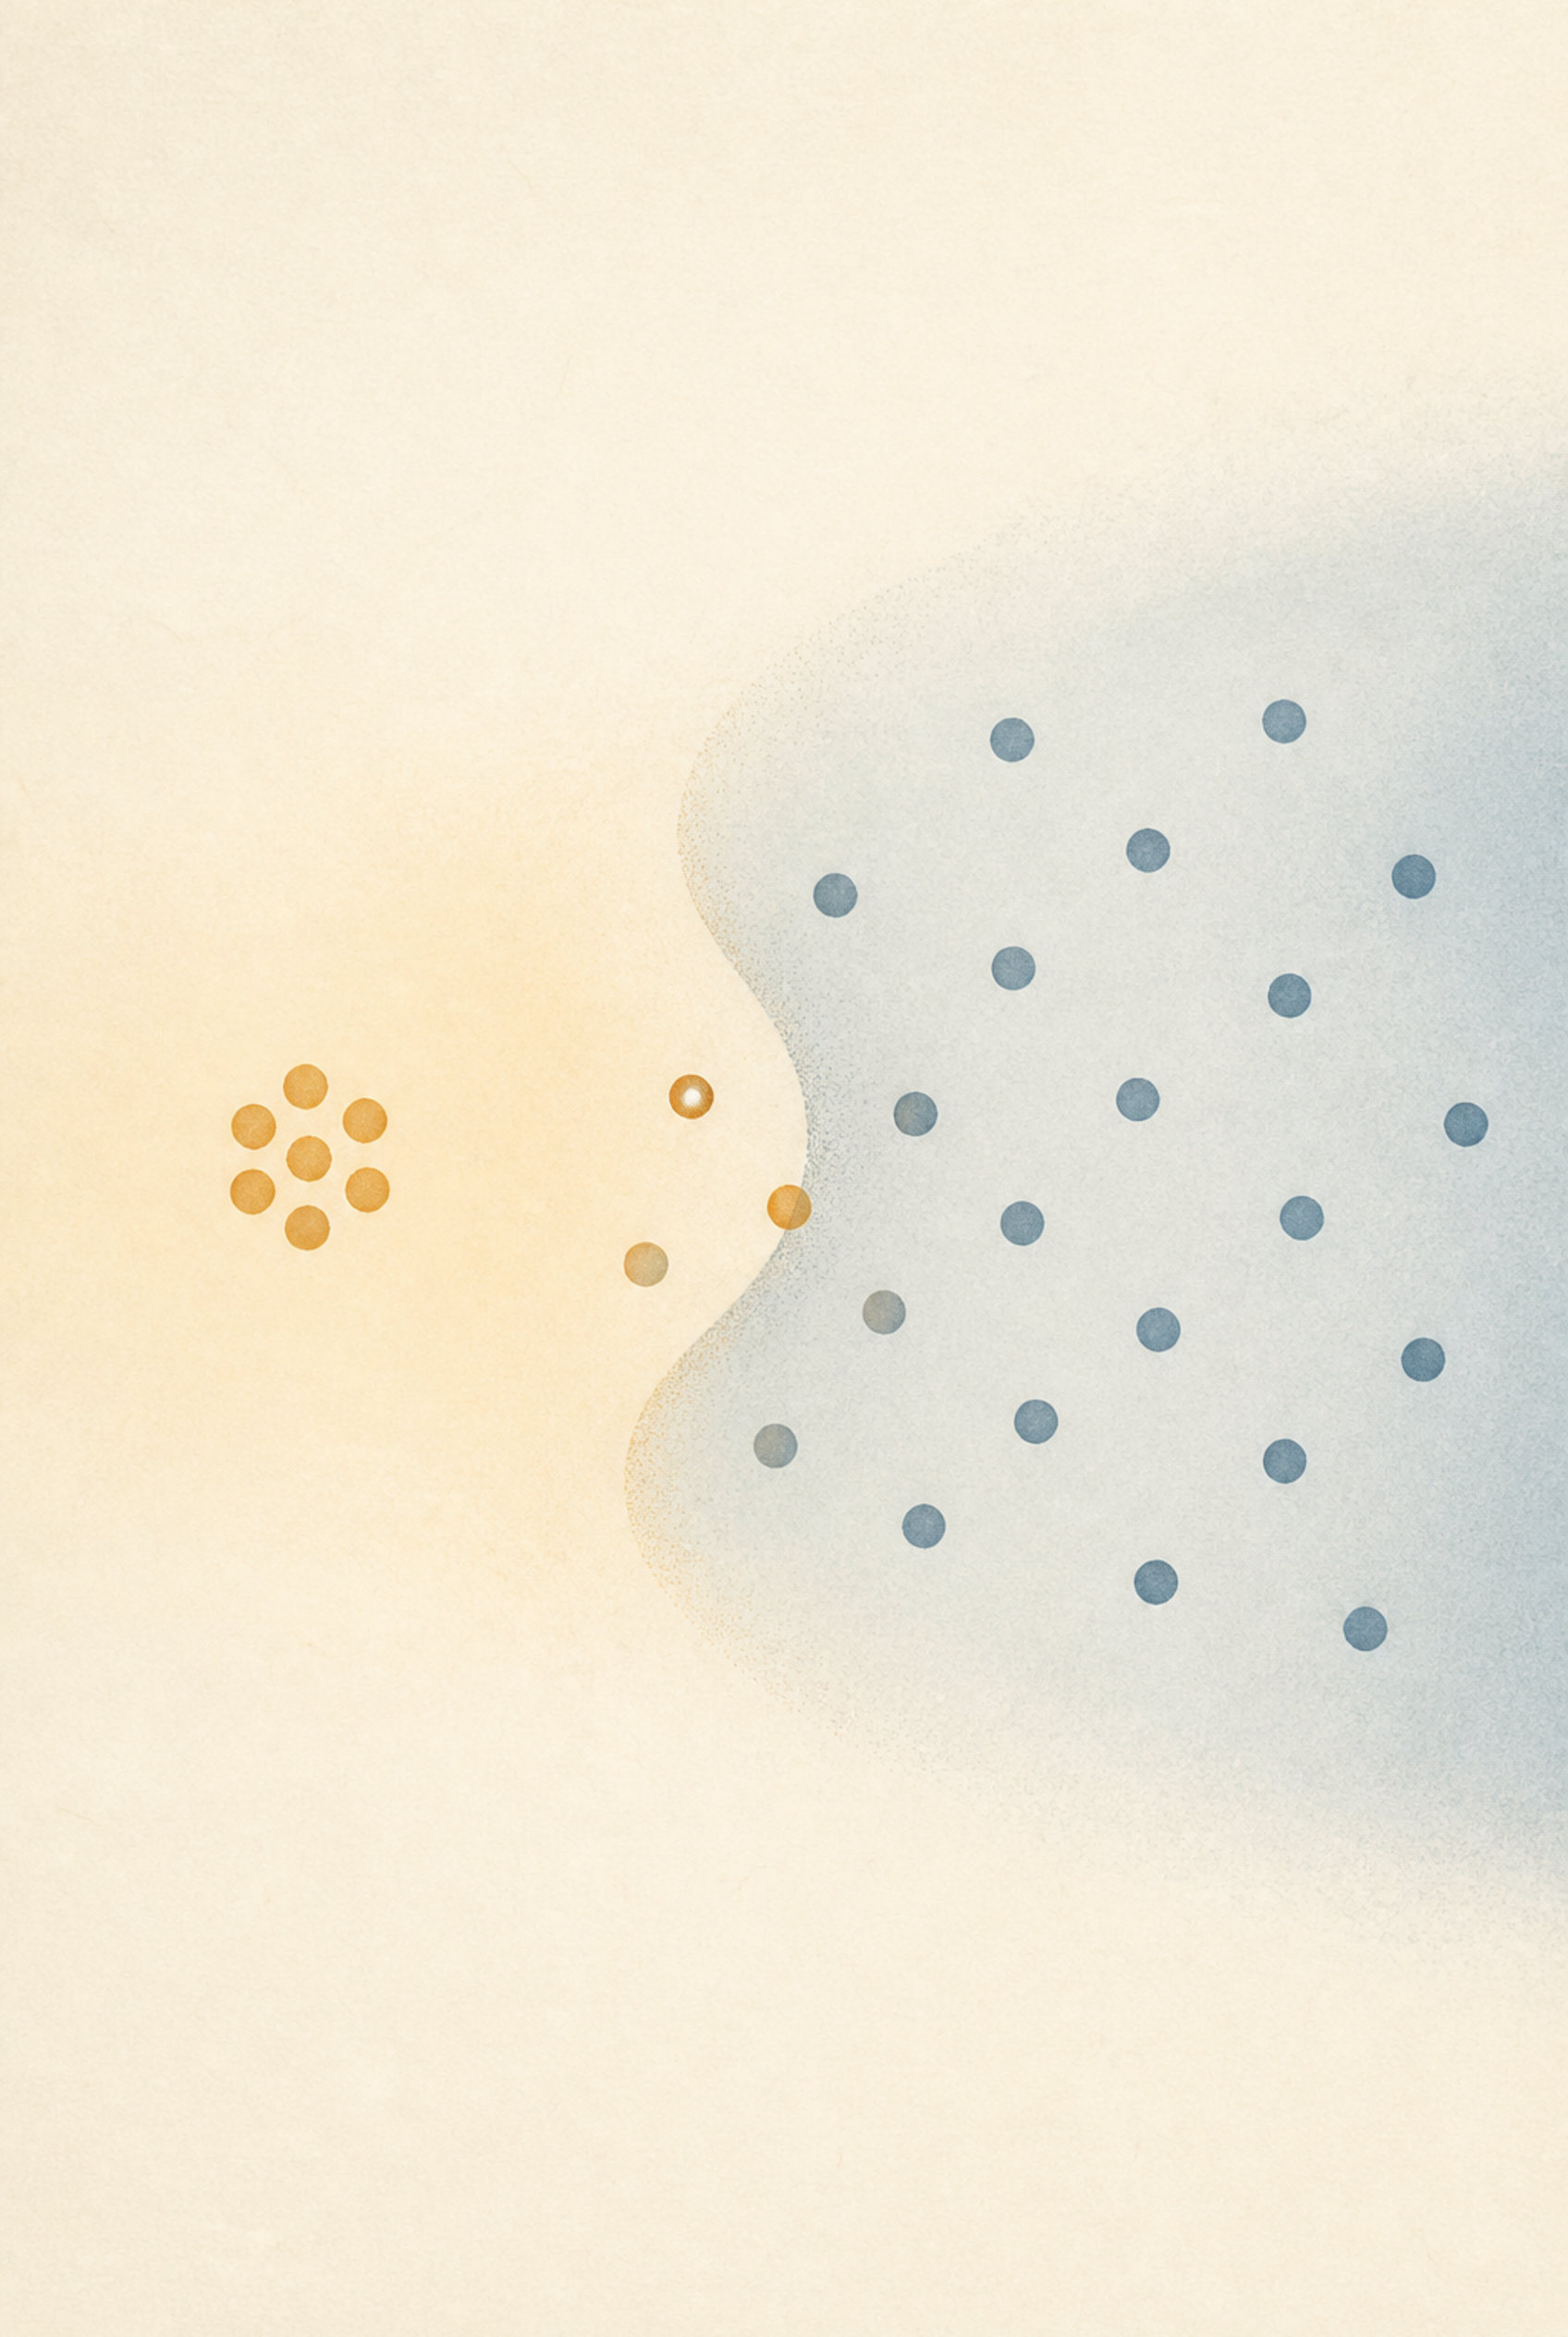
\includegraphics[width=\paperwidth,height=\paperheight,keepaspectratio=false]{../../../generated_course_notes/core/statistical_mechanics/2013_spring_theoretical_minimum/assets/cover-art.png}%
  };
  \node[
    anchor=north west,
    align=left,
    text width=0.78\paperwidth,
    fill=white,
    fill opacity=0.9,
    rounded corners=8pt,
    inner xsep=10pt,
    inner ysep=8pt
  ] at ([xshift=0.08\paperwidth,yshift=-0.06\paperheight]current page.north west) {%
    {\fontsize{30}{33}\selectfont\bfseries\color{black!88} 統計力学\\[0.85em]}
    {\large\color{black!72} 日本語版 / 2013 spring theoretical minimum}
  };
  \node[
    anchor=south west,
    align=left,
    text width=0.68\paperwidth,
    fill=white,
    fill opacity=0.82,
    text opacity=1,
    rounded corners=6pt,
    inner sep=12pt
  ] at ([xshift=0.08\paperwidth,yshift=0.08\paperheight]current page.south west) {%
    {\normalsize\color{black!78} 原講義：Leonard Susskind\\[0.35em]}
    {\small\color{black!72} 講義補助版：\href{https://lazying.art}{LazyingArt LLC} / \href{https://github.com/lachlanchen/Video2Book}{Video2Book}.}
  };
\end{tikzpicture}
\mbox{}
\end{titlepage}
\hypersetup{pageanchor=true}

\chapter*{本ノートについて}
本独立編集のコンパニオンノートは、Leonard Susskindによる2013年の『統計力学』講義に基づくものである。講義の説明順序、実質的な教室でのやり取り、数学的導出、および選ばれた黒板の証拠を保持している。これらはSusskind教授による原著ではなく、同教授による査読や承認を受けていない。

本版は\href{https://lazying.art}{LazyingArt LLC}がオープンソースの\href{https://github.com/lachlanchen/Video2Book}{Video2Book}ワークフローを用いて作成した。完全な機械文字起こしと字幕ファイルはリポジトリ内に別途利用可能な形で残されており、認識誤りを含む可能性がある。
\clearpage
\tableofcontents
\mainmatter
\chapter{確率・情報・エントロピー}

\lectureoverview{統計力学は、微視的法則と不完全な知識とが出会うところから始まる。まず確率を精密に定式化し、次に決定論的運動それ自体がどのように確率を割り当てるのか、保存則がどのように状態空間を分割するのか、そして情報を保存する力学がなぜ自然にエントロピーへと導くのかを問う。第一法則と第零法則が入ってくるのは、この構造が整ってからである。}

\section{なぜ統計力学か}

統計力学はときに古い物理学だと言われる。その説明は的を外している。統計力学は前近代的であり、現代的であり、そして我々が知る理論に取って代わるいかなるポストモダン物理学においても有用であり続けるだろう。個別のモデルは現れては消えるが、熱力学第二法則は繰り返し道標として生き残ってきた。自然についての提案された記述が、秩序をただで作り出したり、情報を根本的に消去したり、閉じた系を不自然に単純な状態へと走らせたりするように見えるときはいつでも、第二法則は何かが取りこぼされていると警告する。

この主題は、新たに発見された粒子ほど華やかには見えないかもしれないが、少なくとも同じくらい深く、はるかに一般的である。気体、液体、固体、放射、ブラックホール、情報、量子場は、いずれも統計的推論を必要とする。実際、粒子を発見するために用いられた実験装置も、それなしには理解できない。何世代もの優れた物理学者が、主たる仕事が別のところにあっても統計力学を習得したのはこのためである。この主題は有用であるだけでなく、際立って美しい。

なぜそれが必要なのかを見るには、力学が与える理想から始めればよい。閉じた系とは、考察の対象となっている宇宙全体か、あるいは周囲が影響を及ぼさないほど十分に孤立した部分系である。その初期条件とその発展法則を知っていれば、古典力学は完全な予測を与える。量子力学は予測できるものを変えるが、それもまた精密に定義された状態と、理論が許す最大限の情報を予測する法則とを持つ。

原理上の予測と有用な理解との間には厳しい違いがある。この部屋のすべての分子の位置と速度の一覧は、途方もなく長く、ほとんど即座に変化し、我々が実際に気にかける問いのほとんどに答えてくれない。したがって、正確な微視的法則は、完全に予測的でありながら同時に実用上は役に立たないことがありうる。

統計力学は、この物理的状況に適用された確率論である。初期条件が完全な精度で知られていないとき、法則が近似的にしか知られていないとき、系が開いているとき、あるいは単に微視的変数の数が多すぎて追跡できないときに、それは必要となる。これらのいずれも予測が弱いことを意味しない。大きな数はしばしば統計的予測を極めて鋭いものにする。

孤立した気体の箱を考えよう。我々はすべての分子の軌道を予測することはできないが、わずかな巨視的データから、圧力、エネルギー、その他多くのバルク量を高い精度で予測できる。不確かなまま残るのは揺らぎである。予測できない瞬間に、ある小さな領域が平均より多くの分子を含み、別の領域がより少なく含むことがある。そのような事象は確率分布の裾に位置する。起こりにくいが、禁じられてはいない。特定の発生の瞬間を予測することなく、そのような揺らぎがどのくらいの頻度で起こるべきかを計算できる。

硬貨投げは同じ区別を示す。十億回の公正な投げでは、表と裏の数はほぼ等しくなる。十分に多く投げれば、表が長く連続することもいつかは起こるが、確率論が予測するのはその頻度であって、あらかじめその時刻を指定することではない。統計力学は、その要素が小さすぎるか、多すぎるか、あるいはその両方である系のために設計されている。

本講義では、法則そのものと物質への応用の両方を展開する。この主題は繰り返し学ぶことに報いてくれる。一度学び、その一部を忘れ、どの考えが基本的であるかについてより深い感覚をもって再び学ぶのである。我々は、続くすべてを支配するその考えから始める。

\section{原始的な言語としての確率}

なぜ確率がうまく働くのかは、確率の計算それ自体が説明するものではない。確率的予測は特定の試行では外れることがある。結果が可能ではあるが起こりにくいとは、そういうことである。理論は例外がどのように分布するかを教える。例外を廃止するのではない。したがって我々は確率を原始的概念として受け入れ、それが従う規則を述べる。

\subsection{状態と規格化}

\(i\) が可能な結果、または系の可能な状態を表すとしよう。1個の硬貨では、\(i\) は表または裏を意味しうる。1個のサイコロでは、\(1\) から \(6\) までの値をとりうる。2個のサイコロでは、添字の対が両方の面を記録する。まず有限の離散的な状態空間から始める。
\begin{equation}
 i=1,\ldots,N,
\end{equation}
そして後に、無限個および連続無限個の状態へ移行する。

無知であるとは、系が状態をもたないという意味ではない。どの状態をもつかを我々が知らないという意味であり、それゆえ各可能性に確率 \(p_i\) を割り当てる。基本規則は
\begin{align}
 p_i &\geq 0, \label{eq:sm1-prob-positive}\\
 \sum_{i=1}^{N}p_i &=1. \label{eq:sm1-prob-normalization}
\end{align}
である。諸選択肢は互いに排反かつ網羅的である。すなわち、そのうちのちょうど1つが生じる。負の確率はここでは役割をもたず、和が1であるのは、許された結果のどれかが必ず生じるからである。

\subsection{頻度と大数の法則}

確率は繰り返し試行によって実験と結びつく。同じ実験を \(N_{\mathrm{trials}}\) 回行い、\(N(i)\) を結果 \(i\) を生じる試行の数としよう。このとき頻度解釈は
\begin{equation}
 p_i=
 \lim_{N_{\mathrm{trials}}\to\infty}
 \frac{N(i)}{N_{\mathrm{trials}}}.
 \label{eq:sm1-frequency}
\end{equation}
である。これは理想的な極限を通じて表された物理的仮説である。無限回の実験を行う実験室は存在しない。主張は、十分に多くの試行を行えば、その比が意図された予測にとって十分近く \(p_i\) に落ち着くというものである。有限の標本は極限値のまわりで変動する。

\subsection{平均値}

次に、各状態に数 \(f(i)\) を割り当てる。それはエネルギー、運動量、あるいは我々が測定したい任意の他の量でありうる。その期待値は
\begin{equation}
 \langle f\rangle=\sum_i f(i)p_i.
 \label{eq:sm1-expectation}
\end{equation}
である。ブラケット記法は量子力学の外でも便利である。頻度の言葉では、同じ平均は
\begin{equation}
 \langle f\rangle
 =
 \lim_{N_{\mathrm{trials}}\to\infty}
 \frac{1}{N_{\mathrm{trials}}}
 \sum_i f(i)N(i).
 \label{eq:sm1-frequency-average}
\end{equation}
である。

硬貨について、
\begin{equation}
 f(\mathrm{H})=+1,
 \qquad
 f(\mathrm{T})=-1.
\end{equation}
と定義する。表と裏がそれぞれ確率 \(1/2\) をもつならば、
\begin{equation}
 \langle f\rangle
 =(+1)\frac12+(-1)\frac12=0.
\end{equation}
である。平均は可能な結果である必要はない。硬貨が0の上に落ちることは決してない。0はその2つの可能な値の分布を要約しているのである。

この短い間奏は、この分野全体で用いられる語彙を確定する。すなわち、状態、確率、頻度、そして期待値である。

\section{確率を割り当てる3つの方法}

\subsection{対称性}

なぜ我々は通常、硬貨の2つの面に等しい確率を割り当てるのか。第一の答えは対称性である。ほぼ理想的な硬貨を裏返すことは、実験を変えることなく表と裏を交換する。そのとき、どちらかの結果を優先する物理的理由はない。実際の刻印や不完全さはわずかな偏りをもたらすが、対称な模型は意図された実験を捉えている。
\begin{equation}
 p(\mathrm{H})=p(\mathrm{T})=\frac12.
\end{equation}

同じ議論により、対称なサイコロの各面に確率 \(1/6\) が与えられる。より一般には、対称性によって関係づけられる配置には、何らかの追加情報がその対称性を破らない限り、等しい確率が割り当てられる。

\subsection{実験}

歪んだサイコロには、6つの面すべてを交換する対称性はない。その場合、対称性だけでは答えは得られない。偏りを予測するより深い力学的模型をもつことはありうるが、そのような模型がなければ、誠実な手続きは実験的である。すなわち、サイコロを多数回投げ、頻度を記録し、それらが安定するのを待ち、得られた確率の表を後の予測に用いるのである。

対称性と実験は競合する定義ではない。それらは確率分布に関する情報の2つの源である。統計力学は対称性に大きく依拠することになるが、力学が第三の道を提供する。

\subsection{決定論的運動からの確率}

6つの色の配置をもつ不規則な物体を想像しよう。それは、確定した更新則に従って、固定された離散的な時間間隔で状態を変える。
\begin{equation}
 R\longrightarrow B\longrightarrow Y\longrightarrow G
 \longrightarrow O\longrightarrow P\longrightarrow R.
 \label{eq:sm1-six-cycle}
\end{equation}
物体自体は幾何学的対称性をもつ必要はない。この法則は、与えられた配置にどの配置が続くかを述べているだけである。

\begin{figure}[htbp]
\centering
\includegraphics[width=0.92\textwidth]{lecture_01_figure_02.png}
\caption{期待値の公式は左の板に残ったままで、6つの決定論的な色の更新が右に列挙されている。}
\lectureframe{00:26:28}
\end{figure}

板のリストは、有向サイクルとして描くとより明瞭である。
\begin{figure}[htbp]
\centering
\begin{tikzpicture}[
  >=Latex,
  state/.style={draw,circle,minimum size=8mm,inner sep=1pt}
]
\node[state] (R) at (90:2.2) {$R$};
\node[state] (B) at (30:2.2) {$B$};
\node[state] (Y) at (-30:2.2) {$Y$};
\node[state] (G) at (-90:2.2) {$G$};
\node[state] (O) at (-150:2.2) {$O$};
\node[state] (P) at (150:2.2) {$P$};
\draw[->] (R) -- (B);
\draw[->] (B) -- (Y);
\draw[->] (Y) -- (G);
\draw[->] (G) -- (O);
\draw[->] (O) -- (P);
\draw[->] (P) -- (R);
\end{tikzpicture}
\caption{単一の6状態軌道。各周期の間にすべての状態が1回ずつ訪れられる。}
\label{fig:sm1-six-cycle}
\end{figure}

初期状態が分からないものとし、未知の時刻にスナップショットを撮るとする。各段階が等しい時間だけ続くので、系は各色に一周期の六分の一ずつを費やす：
\begin{equation}
 p(R)=p(B)=p(Y)=p(G)=p(O)=p(P)=\frac16.
 \label{eq:sm1-uniform-cycle}
\end{equation}
この等式は物体の形に由来するものではない。各状態に費やす時間が等しいことに由来する。

矢印を並べ替えて、依然として1つの6状態サイクルを形成しながら、異なる微視的法則を得ることができる。詳細な順序は変わるが、各状態が依然として周期ごとに1回ずつ生じるので、スナップショットの確率は \(1/6\) のままである。したがってこの予測は、出発点も詳細な順序も必要としない。必要とするのは、軌道構造と更新あたりの等しい時間だけである。

\begin{classroomqa}
\classquestion{対象が対称でない場合、すべての色に確率\(1/6\)を与えることはどのような意味で正当なのか。}
\lecturerresponse{その割り当ては幾何学的というより動力学的である。6段階の軌道の未知の位相で撮られたスナップショットは、6つの等しい時間スロットをサンプリングする。関係する等価性は、対象の面の間ではなく、軌道上の位置の間にある。滞留時間が等しくなければ、確率も等しくならない。
\lecturetimestamp{00:27:11--00:29:49}}
\end{classroomqa}

\section{非連結なサイクルと保存量}

決定論的法則は、すべての状態を1つの軌道に置く必要はない。2つの非連結なサイクルを考える。
\begin{equation}
 R\longrightarrow B\longrightarrow G\longrightarrow R,
 \qquad
 P\longrightarrow Y\longrightarrow O\longrightarrow P.
 \label{eq:sm1-two-cycles}
\end{equation}
系が第1のサイクル上にあるとわかっているなら、
\begin{equation}
 \begin{aligned}
 p(R)=p(B)=p(G)&=\frac13,\\
 p(P)=p(Y)=p(O)&=0.
 \end{aligned}
\end{equation}
第2のサイクル上にあるという知識は、これらの割り当てを逆にする。

より一般的な場合は事前重みを必要とする。サイクルを\(+1\)と\(-1\)とラベル付けし、それらの確率を\(p_+\)と\(p_-\)とする。ただし
\begin{equation}
 p_++p_-=1.
\end{equation}
このとき
\begin{align}
 p(R)=p(B)=p(G)&=\frac{p_+}{3},\\
 p(P)=p(Y)=p(O)&=\frac{p_-}{3}.
 \label{eq:sm1-sector-weights}
\end{align}
因子\(1/3\)はサイクル内の運動から従う。数\(p_+\)と\(p_-\)はそうではない。それらは追加の知識、おそらく初期セクターを選択する別の実験または別の系から来なければならない。

ラベル\(+1\)と\(-1\)は保存量を定義する。いったん系が一方のサイクルで始まれば、更新則がそれを他方へ運ぶことは決してない。この量をエネルギーと呼んでもよいし、\emph{zilch}のような仮の名前を与えてもよい。その名前は二次的である。保存とは、状態空間が力学の越えられない領域に分割されることを意味する。

サイクルは同じ数の状態を含む必要はない。4状態の軌道と2状態の軌道も依然として2つの保存セクターを定義する。このとき等時間サンプリングは、第1のセクター内で\(1/4\)を、第2のセクター内で\(1/2\)を与え、それぞれの場合にそのセクターの事前確率を掛ける。統計力学は論理的に別個の2つの問いに答えなければならない。
\begin{enumerate}
\item 与えられた保存セクターにおいて、力学はその状態にどれだけの時間を費やすか。
\item 保存セクター自体にはどのような確率を割り当てるべきか。
\end{enumerate}

\begin{classroomqa}
\audiencequestion{1つの保存セクター内のすべての状態が同じ確率を受け取ると仮定しているのか。}
\lecturerresponse{ここに示した離散的な玩具法則については、はい。各状態が同じ時間間隔続き、運動が決定論的だからである。無知は軌道の初期位相にある。ミリ秒の時間分解能をもつ検出器はマイクロ秒の更新を分解できないが、十分に速いスナップショットは捉えられた状態を依然として同定できる。より一般的な系では、等しくない滞留時間を明示的に含めなければならない。
\lecturetimestamp{00:36:16--00:37:17}}
\end{classroomqa}

\begin{classroomqa}
\audiencequestion{2つのスナップショットが撮られ、最初のものが一方のサイクルを同定したなら、2番目のものも同じサイクルを同定すべきか。}
\lecturerresponse{はい。まさにそれが保存の意味である。いったん測定が保存量の値を決定すれば、将来の確率はその値に条件付けることができ、他方のセクターの状態は確率ゼロを受け取る。
\lecturetimestamp{00:37:18--00:37:45}}
\end{classroomqa}

\subsection{2つの系の間で共有されるエネルギー}

ここで抽象的なラベルをエネルギーに置き換える。1つの孤立した箱は閉じた系であり、保存されたエネルギーをもつ。2つの孤立した箱は、相互作用しないため、2つの別々に保存されたエネルギーをもつ。エネルギーが流れることを許す狭い通路でそれらを接続すると、全エネルギーは固定されたまま、別々のエネルギーは変化しうる。

\begin{figure}[htbp]
\centering
\includegraphics[width=0.92\textwidth]{lecture_01_figure_03.png}
\caption{エネルギーが通過できる狭いチャネルで接続された2つの部分系。}
\lectureframe{00:39:19}
\end{figure}

\begin{figure}[htbp]
\centering
\begin{tikzpicture}[>=Latex]
\draw[thick,rounded corners=4pt] (-4,1.8) rectangle (-0.7,-1.5);
\draw[thick,rounded corners=4pt] (0.7,1.5) rectangle (4,-1.8);
\draw[thick] (-0.7,0.45) -- (0.7,0.45);
\draw[thick] (-0.7,-0.35) -- (0.7,-0.35);
\draw[<->,very thick] (-0.45,0.05) -- (0.45,0.05);
\node at (-2.35,0.15) {subsystem \(1\)};
\node at (2.35,-0.15) {subsystem \(2\)};
\node[above] at (0,0.5) {energy exchange};
\end{tikzpicture}
\caption{接続が開かれると、\(E_1+E_2\)だけが保存される。エネルギーの分割は確率の問題になる。}
\label{fig:sm1-connected-systems}
\end{figure}

全エネルギーが与えられたとき、部分系\(1\)が\(E_1\)をもち、部分系\(2\)が残りをもつ確率を問うことができる。等しい箱は平均して等しいエネルギーをもつべきだが、平均は分布の全体ではない。したがって部分系の確率を決定する1つの方法は、それをより大きな閉じた系に埋め込み、その保存則が欠けている情報を与えるようにすることである。この構成は統計力学の至るところで再び現れる。

\section{良い法則、悪い法則、そしてマイナス第一法則}

すべての決定論的更新則が基礎法則として許されるわけではない。写像
\begin{equation}
 \begin{aligned}
 R&\mapsto R,& B&\mapsto R,& Y&\mapsto R,\\
 G&\mapsto R,& O&\mapsto R,& P&\mapsto R.
 \end{aligned}
 \label{eq:sm1-all-to-red}
\end{equation}
を考える。これは未来を完全に予測する。1ステップ後、状態は赤である。しかし逆方向では失敗する。系が赤になると、青、黄、緑、橙、紫、または赤自身から来たのかを何も明かさない。

\begin{figure}[htbp]
\centering
\begin{tikzpicture}[
  >=Latex,
  state/.style={draw,circle,minimum size=8mm,inner sep=1pt}
]
\node[state,fill=red!12] (R) at (0,0) {$R$};
\node[state] (B) at (-3,1.6) {$B$};
\node[state] (Y) at (-3,0) {$Y$};
\node[state] (G) at (-3,-1.6) {$G$};
\node[state] (O) at (3,1.6) {$O$};
\node[state] (P) at (3,-1.6) {$P$};
\draw[->] (B) -- (R);
\draw[->] (Y) -- (R);
\draw[->] (G) -- (R);
\draw[->] (O) -- (R);
\draw[->] (P) -- (R);
\draw[->,loop above] (R) to (R);
\end{tikzpicture}
\caption{多対一の法則は次の状態を予測するが、可能な過去の状態の間の区別を消去する。}
\label{fig:sm1-bad-law}
\end{figure}

対照的に、閉じたサイクルは記録を保存する。経過時間がわかっていれば、何千周期も経た後でさえ、状態を未来へも過去へも発展させることができる。法則は初期条件の間の区別を保存する。Susskindはこの要請を\emph{物理学の第一法則に対するマイナス}と呼ぶ。情報は根本的には失われないのである。

有限の離散状態空間に対しては、図式的な判定基準は単純である。
\begin{quote}
良い法則の各状態は、ちょうど1本の出ていく矢印と、ちょうど1本の入ってくる矢印をもつ。
\end{quote}
出ていく矢印が未来を決定し、入ってくる矢印が過去を再構成する。数学的には、更新は状態の置換である。

\subsection{摩擦は見かけ上の反例にすぎない}

連続的な対応物はLiouvilleの定理である。摩擦はこれに矛盾するように見える。消しゴムを机の上で滑らせると、消しゴムがどこから出発しても、やがて静止する。模式的な抗力方程式は
\begin{equation}
 m\ddot x=-\gamma\dot x,
 \qquad \gamma>0.
 \label{eq:sm1-drag}
\end{equation}
であり、その速度は指数関数的に減衰する。もしこれが密閉された部屋の中のあらゆる粒子の根本法則であるなら、すべての運動は消え去り、温度はゼロまで下がり、多くの初期状態が1つの最終状態へと崩壊することになる。エネルギー保存は破れ、情報は消え、無秩序は減少する。これは、すべてが赤へ向かうことの連続版であろう。

実際の摩擦はこのようにはならない。消しゴムは机と、それ自身と、周囲の環境とを温める。微視的な位置と運動量が、可視的な運動から失われた区別を記録する。摩擦は、観測されない自由度が省略された後の部分系に対する有効方程式であり、完全な閉じた系に対する根本的な散逸法則ではない。

\begin{classroomqa}
\classquestion{微分方程式
\(m\ddot x=-\gamma\dot x\)は何を表し、なぜ根本的な閉じた系の法則ではないのか。}
\lecturerresponse{それは粘性抗力の方程式である。それ自体ではあらゆる速度をゼロへと駆り立て、初期温度にかかわらず気体をゼロまで冷却させることになる。実際の閉じた記述では、失われた力学的エネルギーと情報は微視的な自由度へと移る。抗力方程式は、それらの変数が抑圧された後にのみ信頼できる。
\lecturetimestamp{00:44:40--00:48:56}}
\end{classroomqa}

\section{占有状態と最初のエントロピー}

情報保存には等価な確率的な言明がある。\(N\)個の状態のうち\(M\)個に等しい確率が割り当てられているとしよう。
\begin{equation}
 p_i=
 \begin{cases}
 1/M, & i\text{ in the occupied set},\\
 0, & i\text{ outside it}.
 \end{cases}
 \label{eq:sm1-uniform-occupied}
\end{equation}
情報を保存する更新は、どの状態が占有されているかを入れ替えることはあっても、それらを融合させることはできない。それ以降のどの時刻でも、依然として確率\(1/M\)をもつ\(M\)個の状態がある。これに対して、悪い写像\eqref{eq:sm1-all-to-red}は、多くの占有状態を1つに崩壊させうる。

数\(M\)は無知を測る。\(M=N\)ならば、あらゆる状態が可能であり、我々の無知は最大である。\(M=1\)ならば、微視的状態は正確にわかっている。したがってエントロピーの最初の定義は
\begin{equation}
 S=\log M.
 \label{eq:sm1-entropy-logm}
\end{equation}
であり、これは
\begin{equation}
 S_{\max}=\log N,
 \qquad
 S_{\min}=0.
\end{equation}
を与える。状態空間が無限であれば、有限の上限が存在する必要はない。

この展開では、エントロピーは温度より前に現れ、エネルギーの保存の形式的な言明よりもさらに前に現れる。その意味でそれはより原始的である。しかしそれは力学的系だけの性質ではない。それは系と、何が知られているかを表す確率分布とに共同で依存する。同じ力学的系でも、異なる情報をもつ観測者によって異なるエントロピーを割り当てられうる。

厳密な微視的発展の下では、占有状態は並べ替えられるだけなので、この細粒エントロピーは保存される。実際には我々はタイミングを失い、相関を捨て、膨大な数の変数を追跡し損なう。すると我々の確率分布はより多くの選択肢に広がり、粗い記述に割り当てられたエントロピーは増大する。我々の使える記述が情報を失うために、方程式が情報を破壊する必要はない。

\begin{classroomqa}
\classquestion{\(N\)個の状態をもつ有限系の最大可能エントロピーは何か。}
\lecturerresponse{それは\(\log N\)であり、\(N\)個の状態がすべて等確率のときに達成される。最小のエントロピーはゼロであり、1つの状態が確率1をもつときに達成される。したがってエントロピーは、利用可能な状態空間だけでなく、知識の状態をも測る。
\lecturetimestamp{00:56:46--00:58:19}}
\end{classroomqa}

\section{連続位相空間におけるLiouvilleの流れ}

連続的な位置と運動量をもつ粒子の場合、微視的状態は相空間の一点である。座標を\(q_a\)、その共役運動量を\(p_a\)と書く。粒子が多数になると軸の数は膨大になり、一つの\(q\)と一つの\(p\)をもつ二次元の図はあくまで代用にすぎない。すべての座標には運動量の相棒が存在するため、相空間は偶数次元である。

我々の知識が領域\(\Omega_0\)によって表されるとしよう。確率密度はその領域の内部で一様であり、外部ではゼロである。例えば、すべての粒子が部屋の中にあるという知識は位置座標を制限し、それらの速さに対する上限は運動量座標を制限する。

ハミルトン的発展は各相空間点を軌道に沿って運ぶ。近傍の点は近傍の点へと移り、占有された領域は非圧縮性流体の一片のように流れる。
\begin{figure}[htbp]
\centering
\begin{tikzpicture}[>=Latex,scale=0.95]
\draw[->] (-4.2,0) -- (4.3,0) node[right] {$q$};
\draw[->] (-3.7,-2.2) -- (-3.7,2.4) node[above] {$p$};
\draw[fill=blue!12,thick]
  (-3.0,-0.5) .. controls (-2.7,1.0) and (-1.3,1.2) .. (-0.9,0.1)
  .. controls (-0.6,-1.0) and (-2.2,-1.4) .. cycle;
\node at (-1.9,0.0) {$\Omega_0$};
\draw[->,very thick] (-0.3,0.2) -- (0.8,0.2);
\draw[fill=orange!15,thick]
  (1.2,-1.1) .. controls (1.5,0.3) and (2.3,1.8) .. (3.2,1.1)
  .. controls (3.6,0.7) and (2.8,-0.4) .. (2.5,-1.5)
  .. controls (2.1,-1.8) and (1.5,-1.6) .. cycle;
\node at (2.35,0.1) {$\Omega_t$};
\end{tikzpicture}
\caption{ハミルトン的流れは占有された相空間領域を伸長し剪断しうるが、その体積は保存する。}
\label{fig:sm1-liouville-flow}
\end{figure}

リウヴィルの定理は
\begin{equation}
 \operatorname{Vol}(\Omega_t)
 =
 \operatorname{Vol}(\Omega_0).
 \label{eq:sm1-liouville-volume}
\end{equation}
と述べる。初期密度が\(\Omega_0\)上で一様ならば、輸送された密度は\(\Omega_t\)上で一様である。これは占有された離散状態の数と重みを保存することの連続的類似物である。

この定理はまた、摩擦のパズルを幾何学的に解決する。消しゴムの可視的な運動量のみに注目すると、可能性の雲は\(p=0\)へと絞られていくように見える。完全な相空間では、その雲は消しゴムと机の分子の位置と運動量へと広がる。射影は収縮しうるが、完全な高次元体積は一定のままである。

\begin{classroomqa}
\classquestion{すべての可視的な軌道が静止に近づくならば、占有された相空間領域は軸\(p=0\)上に崩壊したのか。}
\lecturerresponse{縮約された射影においてのみである。完全な系は机、消しゴム、そして周囲の微視的変数を含む。可視的な運動量の範囲が狭まるにつれて、分布はそれらの隠れた方向へと広がる。リウヴィルの定理は完全な閉じた相空間に適用され、巨視的変数の不完全な集合には適用されない。
\lecturetimestamp{01:04:37--01:06:29}}
\end{classroomqa}

\section{マイナス第一法則から第一法則へ}

\subsection{第零法則の簡単な考察}

第一法則を述べる前に、第零法則に名前を与えておくと有用である。熱平衡はまだ定義されていないので、今のところこの法則は構造的な言明にすぎない。
\begin{quote}
系\(A\)が\(B\)と熱平衡にあり、\(B\)が\(C\)と熱平衡にあるならば、\(A\)は\(C\)と熱平衡にある。
\end{quote}
この推移性が後に温度を可能にする。今はこれを脇に置く。

\subsection{エネルギー保存}

閉じた系に対する第一法則は単に
\begin{equation}
 \frac{dE}{dt}=0.
 \label{eq:sm1-first-law}
\end{equation}
である。その簡潔な形はその力を隠している。エネルギーは保存量であり、エネルギーという語は後にさらに多くの熱力学的内容を獲得するであろう。

閉じた系が二つの部分からなり、それらのエネルギーが加法的であるならば、
\begin{equation}
 E=E_1+E_2,
\end{equation}
したがって
\begin{equation}
 \frac{dE_1}{dt}+\frac{dE_2}{dt}=0,
 \qquad\text{or}\qquad
 \frac{dE_1}{dt}=-\frac{dE_2}{dt}.
 \label{eq:sm1-energy-exchange}
\end{equation}
第二の形は交換を明示する。一方の部分系が失ったエネルギーは他方が得る。

加法性の仮定には注意が必要である。二つの重力を及ぼし合う粒子は個々の運動エネルギーを持つが、それらの相互作用はその対に属するポテンシャルエネルギーに寄与する。全エネルギーは保存されるが、それを一方の物体のエネルギーと他方のエネルギーの和として厳密に書くことはできない。

熱力学ではしばしば優れた加法的近似が許される。なぜなら、バルクのエネルギーは体積に比例してスケールする一方、大きな隣接部分間の短距離相互作用エネルギーは主にそれらの接触面積に比例してスケールするからである。大きな机をブロックに分割しよう。各ブロックの内部エネルギーは体積効果であり、隣接ブロック間の結合は表面効果である。大きなブロックでは、後者は比較的小さい。式
\eqref{eq:sm1-first-law}は閉じた全体に対して厳密であり、部分系の形
\eqref{eq:sm1-energy-exchange}は相互作用エネルギーが無視できることを仮定している。

\begin{classroomqa}
\audiencequestion{規格化\(\sum_i p_i=1\)も、列挙された結果が互いに排他的であることを仮定しているのか。}
\lecturerresponse{はい。状態ラベルは選択肢が重ならないように定義される。すなわち、サイコロが黄色の状態にあるならば、同時に赤の状態にはない。通常の言葉では色は混ざりうるが、確率計算で用いられる状態分割は互いに排他的な選択肢からなっていなければならない。
\lecturetimestamp{01:12:14--01:12:55}}
\end{classroomqa}

\section{エントロピーへ戻る}

講義はここで未完了の課題へ明示的に戻る。温度は感覚には馴染み深いが、導出された量である。温度を清潔に定義する前に、エントロピーとエネルギーが整っていなければならない。

\subsection{一般的な確率分布}

特別な定義\(S=\log M\)は、\(M\)個の状態が等確率であり、他のすべてが確率ゼロである場合に適用される。一般的な分布は矩形である必要はない。その重みは状態ラベルにわたって滑らかに、あるいは不規則に変化しうる。

\begin{figure}[htbp]
\centering
\includegraphics[width=0.92\textwidth]{lecture_01_figure_05.png}
\caption{離散的な状態ラベル上に描かれた確率分布。エントロピーに必要な特徴は、正確な曲線ではなく、広がりである。}
\lectureframe{01:14:40}
\end{figure}

\begin{figure}[htbp]
\centering
\resizebox{\linewidth}{!}{%
\begin{tikzpicture}[>=Latex,scale=0.93]
\draw[->] (-4.2,0) -- (4.4,0) node[right] {state label \(i\)};
\draw[->] (-4,0) -- (-4,3.2) node[above] {$p_i$};
\foreach \x in {-3.6,-3.1,...,3.6}
  \draw (\x,0.08) -- (\x,-0.08);
\draw[very thick]
  plot[smooth] coordinates {
  (-3.7,0.12) (-3.0,0.28) (-2.3,0.72) (-1.6,1.45)
  (-0.9,2.25) (-0.2,2.65) (0.5,2.28) (1.2,1.55)
  (1.9,0.88) (2.7,0.38) (3.5,0.14)};
\draw (-1.8,-0.18) -- (-1.8,-0.5);
\draw (1.8,-0.18) -- (1.8,-0.5);
\draw[<->] (-1.8,-0.46) -- (1.8,-0.46);
\node at (0,-0.82) {effective spread};
\end{tikzpicture}
}
\caption{狭い分布は広い分布よりも不確かさが小さい。エントロピーは分布を全体として測らなければならない。}
\label{fig:sm1-probability-spread}
\end{figure}

一般的な定義は
\begin{equation}
 S=-\sum_i p_i\log p_i.
 \label{eq:sm1-shannon-entropy}
\end{equation}
である。\eqref{eq:sm1-expectation}を用いると、これは
\begin{equation}
 S=-\langle\log p\rangle.
\end{equation}
となる。負号は、\(0<p_i<1\)のとき\(\log p_i<0\)であるという事実を補償する。

\subsection{一様な結果の回復}

一般式が最初の定義を再現することを確認しなければならない。空の状態では、\(p_i=0\)である一方、\(\log p_i\)は発散する。その積はよく定義された極限値
\begin{equation}
 \lim_{p\to0^+}p\log p=0.
 \label{eq:sm1-plogp-limit}
\end{equation}
を持つ。したがって、確率ゼロの状態は何も寄与しない。

\begin{classroomqa}
\audiencequestion{もし\(p_i=0\)ならば、その項は本当に消えるのか？ゼロの対数は負の無限大である。}
\lecturerresponse{その項は極限
\(\lim_{p\to0^+}p\log p\)によって定義され、これはゼロである。因子\(p\)は対数が発散するよりも速くゼロに近づく。ゆえに、任意に確率の低い状態は任意に小さな寄与をなし、厳密に不可能な状態は何も寄与しない。
\lecturetimestamp{01:18:27--01:19:46}}
\end{classroomqa}

\(M\)個の占有状態のそれぞれについて、\(p_i=1/M\)である。したがって
\begin{align}
 S
 &=-\sum_{\mathrm{occupied}\ i}
 \frac1M\log\!\left(\frac1M\right)\\
 &=-M\frac1M\log\!\left(\frac1M\right)\\
 &=-\log\!\left(\frac1M\right)
 =\log M.
 \label{eq:sm1-entropy-check}
\end{align}
一般式は特別な式と厳密に一致する。より広い分布はより多くの選択肢に無視できない重みを与え、したがってより大きなエントロピーを持つ。より狭い分布はより小さなエントロピーを持つ。

\begin{figure}[htbp]
\centering
\includegraphics[width=0.92\textwidth]{lecture_01_figure_06.png}
\caption{マークされた幅\(M\)は、有意な確率の広がりとエントロピーの間の関係を強調する。}
\lectureframe{01:16:42}
\end{figure}

エントロピーは状態空間上の確率分布に属する。それは一つの微視的状態のエネルギーや運動量のような裸の観測量ではない。厳密な状態はその状態に集中した分布で表され得て、そのときエントロピーはゼロであるが、知識の状態が変わればエントロピーは変化する。

\section{コイン、ビット、明示的な数え上げ}

\(n\)をコインの枚数とする。微視的配置の数は
\begin{equation}
 N=2^n.
 \label{eq:sm1-coin-state-count}
\end{equation}
である。コインについて何も知られていなければ、\(2^n\)個の配置はすべて等確率であり、
\begin{equation}
 S_{\max}=\log(2^n)=n\log2.
 \label{eq:sm1-coin-max-entropy}
\end{equation}
となる。エントロピーは独立なコインの枚数について加法的である。

\(2\)を底とする対数では、完全に未知の二状態系はエントロピー1ビットを持つ。自然対数では、エントロピー\(\log2\)を持つ。単位は慣習的なものであり、根底にある順序と加法性は変わらない。

もう一方の極端では、すべてのコインが既知ならば、ちょうど一つの配置が確率1を持つ：
\begin{equation}
 S=0.
\end{equation}
より多くの知識はより少ないエントロピーを意味する。

次に、\(n\)枚のコインのうちちょうど一枚が裏で、他はすべて表であり、裏の位置が未知であると仮定する。裏の可能な位置ごとに一つずつ、\(n\)個の等確率な配置があるので、
\begin{equation}
 S=\log n.
 \label{eq:sm1-one-tail-entropy}
\end{equation}
となる。これは一般に\(\log2\)の整数倍ではない。ビットは便利な単位であり、すべてのエントロピーが整数ビット刻みで生じるという主張ではない。

\begin{classroomqa}
\audiencequestion{\(\log2\)が現れるのは、各コインが二つの可能な状態を持つからだけなのか？三状態の要素なら\(\log3\)を与えるのか？}
\lecturerresponse{その通り。\(k\)個の可能な状態を持つ一様に未知の要素は\(\log k\)を寄与する。二値スイッチは、物理的スイッチが自然に二つの安定状態を実現するため、また二が最小の非自明な整数であるため、コンピュータにおいて特に便利である。
\lecturetimestamp{01:29:55--01:30:48}}
\end{classroomqa}

\begin{classroomqa}
\audiencequestion{対数にはどの底が意図されているのか？}
\lecturerresponse{これらの物理の公式では、\(\log\)は自然対数を意味する。情報理論家はしばしば底\(2\)を用いるので、エントロピーは直接ビットで測られる。底を変えることはすべてのエントロピーを一つの固定された換算係数で掛け、物理的結論を何も変えない。
\lecturetimestamp{01:30:49--01:32:06}}
\end{classroomqa}

\section{連続相空間におけるエントロピー}

古典相空間\(\Gamma\)に戻る。確率密度が体積\(V_\Gamma\)の領域上で一様で外部でゼロならば、\(M\)個の等確率状態を数えることの類似は
\begin{equation}
 S=\log\!\left(\frac{V_\Gamma}{V_0}\right).
 \label{eq:sm1-continuous-uniform}
\end{equation}
である。ここで\(V_\Gamma\)は座標と運動量の完全な高次元空間における体積であり、通常の空間体積ではない。固定された体積\(V_0\)は、対数を無次元にする参照相空間セルである。\(V_0=1\)と置くと、板書で用いられる略記\(S=\log V_\Gamma\)を与える。

一般の確率密度\(P(q,p)\)に対して、離散和は相空間積分になる。規格化は
\begin{equation}
 \int_\Gamma d\Gamma\,P(q,p)=1,
 \label{eq:sm1-continuous-normalization}
\end{equation}
であり、エントロピーは
\begin{equation}
 S=-\int_\Gamma d\Gamma\,
 P(q,p)\log\!\bigl[P(q,p)V_0\bigr].
 \label{eq:sm1-continuous-entropy}
\end{equation}
である。密度は相空間のセルあたりの確率である。概念的には、\eqref{eq:sm1-continuous-entropy}は依然として確率がどれだけ広く分布しているかを測っており、一様な塊に対しては、基準セルを単位として測った占有体積の対数に帰着する。その固定されたセルを変えると、すべての連続エントロピーが同じ加法定数だけずれ、エントロピー差は変わらない。

\begin{classroomqa}
\audiencequestion{なぜ座標記号が\(x\)から\(q\)に変わったのですか。}
\lecturerresponse{物理的な変化はない。古典力学では座標に\(x\)または\(q\)を、共役運動量に\(p\)を用いることがよくある。記法の切り替えは単なるミスであり、相空間の構成は同じである。
\lecturetimestamp{01:37:10--01:37:39}}
\end{classroomqa}

温度とボルツマン分布は意図的に後回しにされる。次の課題は熱平衡を定義し、次にその確率分布を特定することである。

\section{相関、加法性、情報に関する質問}

\subsection{相関とは、一方の測定が他方の分布を変えることである}

独立なコインについて完全に無知である場合、すべての配置に等しい確率を割り当てる。すると、1枚のコインを測定しても他のどのコインについても何もわからない。それらの分布は変わらない。

片側テールのアンサンブルは異なる。測定したコインが裏なら、他のすべてのコインは確実に表である。測定したコインが表なら、唯一の裏は残りの\(n-1\)枚のコインの中になければならないので、残りの各位置は条件付き確率
\begin{equation}
\begin{aligned}
 p(&\text{tail at a specified remaining position}\\
   &\mid\text{measured head})=\frac{1}{n-1}.
\end{aligned}
 \label{eq:sm1-conditional-tail}
\end{equation}
をもつ。これが相関である。すなわち、1つの変数を知ることが、別の変数に割り当てられる確率分布を変える。

\begin{classroomqa}
\audiencequestion{エントロピーの例では、コイン間の独立性が仮定されていましたか。}
\lecturerresponse{完全な無知がすべての\(2^n\)個の配置に等しい確率で表された場合に限る。その場合、1枚のコインを測定しても他のコインの分布は変わらない。片側テールの例は明示的に相関しており、測定は他の場所で何が可能かを更新する。述べられた情報が、どの確率分布を用いているかを決める。
\lecturetimestamp{01:38:43--01:41:58}}
\end{classroomqa}

非連結サイクルの例も同じ論理形式をもつ。保存された\(+1\)または\(-1\)のラベルを測定すると、それ以降のすべての状態が1つのセクターに制限される。保存情報で条件付けると、許される分布が変わる。

エントロピーは無相関な系に対して加法的である。もし
\begin{equation}
 p_{ij}=p_i^{(A)}p_j^{(B)},
\end{equation}
ならば
\begin{align}
 S_{AB}
 &=-\sum_{i,j}p_i^{(A)}p_j^{(B)}
 \log\!\left[p_i^{(A)}p_j^{(B)}\right]\\
 &=S_A+S_B.
 \label{eq:sm1-entropy-additivity}
\end{align}
である。相関はこの因数分解を妨げ、対の独立な不確かさを減らす。

演習として、二値変数の列を考えよう。ある変数が上向き状態にあると、各隣接変数が下向きである確率が四分の三になるものとする。一つのサイトを測定すると、近傍のサイトについて知られていることが直ちに変化する。このような分布は相関をもち、そのエントロピーは、それらの相関を考慮に入れずに孤立した一サイトのエントロピーを足し合わせるだけでは求められない。

\subsection{ボルツマン、シャノン、量子不確定性}

\begin{classroomqa}
\audiencequestion{古い熱力学的エントロピーは、シャノンの情報理論的エントロピーとどのように関係していますか。}
\lecturerresponse{同じ関数形が両方に現れる。
\(-\sum_i p_i\log p_i\)。シャノンは通常底\(2\)を用いたが、物理学者は通常自然対数を用い、エントロピーを熱力学的単位で表すときにはボルツマン定数を戻す。数学的な違いは固定された換算係数だけであるが、確率を与える物理的な問いは大きく異なりうる。
\lecturetimestamp{01:44:05--01:46:06}}
\end{classroomqa}

等確率のミクロ状態に対して、熱力学的公式はしばしば
\begin{equation}
 S_{\mathrm{thermo}}=k_{\mathrm B}\log W,
 \label{eq:sm1-boltzmann-formula}
\end{equation}
と書かれる。ここで\(W\)は到達可能なミクロ状態の数である。\(k_{\mathrm B}=1\)とする単位では、これはまさに\(S=\log W\)である。ボルツマン定数は温度の単位とエネルギーの単位を換算する。温度の自然な微視的スケールはエネルギーである。

\begin{classroomqa}
\audiencequestion{このエントロピーは単にハイゼンベルクの不確定性原理の別の形ですか。}
\lecturerresponse{いいえ。ここでのエントロピーは、可能な状態上の確率分布における不確かさを測る。量子論の言葉では、それは混合状態の不確かさであり、純粋状態でも残りうる本質的な測定の不確かさではない。この2つの概念は区別して保たなければならない。
\lecturetimestamp{01:46:07--01:47:31}}
\end{classroomqa}

\section{確立されたこと}

出発点は法則におけるランダム性ではなかった。決定論的力学は、初期状態に関する不完全な知識と結び合わされるだけで、すでに確率を生み出す。単一の軌道は各状態に費やされる時間を通じて重みを割り当てる。互いに連結していない軌道は保存量を明らかにし、各セクター間の事前重みを必要とする。許容される微視的法則は区別を保ち、有限状態空間ではこれが各状態における一本の入る矢印と一本の出る矢印を意味し、連続力学ではリウヴィルの定理となる。

その構造はまず、\(M\) 個の等確率で占有された状態に対して
\begin{equation}
 S=\log M
\end{equation}
を導き、次に
\begin{equation}
 S=-\sum_i p_i\log p_i,
\end{equation}
へ、そして最終的にその相空間積分へと導く。エントロピーは確率分布を、したがって知識の状態を記録する。細粒情報は、実用的な粗粒化記述がその追跡を見失う場合でも、微視的法則によって保存される。

エネルギー保存は第一法則を与えるが、部分系のエネルギーの加法性は相互作用エネルギーが無視できることを要求する。エントロピーは並列的な条件の下で加法的である。すなわち、部分系の確率が無相関でなければならない。これら二種類の加法性が次の段階を準備する。そこでは、熱平衡、温度、ボルツマン分布がエネルギーを確率へと結びつけるであろう。
\chapter{エントロピーとエネルギーから見た温度}

\lectureoverview{温度は、まず人間の温度計の単位を微視的なエネルギーの単位へ変換するものとして現れる。熱力学的エントロピーから無次元の統計的エントロピーへの対応する変換を行った後、我々は平衡状態を1つのパラメータで表される確率分布の族によって記述する。その導関数\(dE/dS\)が温度を定義し、最初の2つの法則は、なぜ温度差がエネルギーの流れの向きを決めるのかを示している。}

\section{換算係数と人間の単位}

物理学の多くの定数は換算係数である。光速は距離を時間に変換する：
\begin{equation}
 t=\frac{x}{c}.
\end{equation}
距離と時間が整合した単位で測られるならば、\(c=1\)と置いてよい。物理的効果は何も消えず、2種類の測定が単に1つの共通の尺度に置かれただけである。

ボルツマン定数も同じ性格をもつ。それは人間の尺度の温度計で読み取られる温度をエネルギーに変換する。\emph{人間の尺度の}という形容詞は重要である。そのような単位は、巨視的な計器が生成し分解できるという理由で選ばれており、微視的な力学がそれらを特別に選び出しているからではない。

摂氏度は、標準圧力における水の凝固点と沸点の間の間隔を100等分することによって定められた。ケルビンは同じ大きさの度を用いるが、零点を絶対零度に置く。異なる物質、異なる間隔、あるいは華氏度を選べば数値は変わるが、物理は変わらない。

\begin{classroomqa}
\audiencequestion{華氏の目盛りはすでに17世紀の構築物だったのか。}
\lecturerresponse{正確な年代はここでは必要ない。要点は、そのような目盛りはすべて、人々が用意し測定できる温度を中心に設計されたということである。それらの度の大きさは微視的というより慣習的である。
\lecturetimestamp{00:01:34--00:01:50}}
\end{classroomqa}

これらの目盛りが作られた当時、熱の分子的起源は実験に利用できなかった。1度の変化は巨視的な温度計で観測できたが、1分子のエネルギーは測定できなかった。したがって、温度が根本的にはエネルギーの尺度であると誰も知る前に、温度の単位を発明するのは自然であった。

\section{なぜ温度はエネルギーの単位をもつのか}

希薄な単原子気体を考える。希薄とは、ここでの目的のためには分子間の相互作用エネルギーを無視してよいことを意味する。熱平衡においては、エネルギー等分配則により、並進運動の各二次の自由度に\(T_{\mathrm K}/2\)とボルツマン定数の積が割り当てられる。三次元空間では、\begin{equation}
 \left\langle E_{\mathrm{kin}}\right\rangle
 =\frac{3}{2}k_{\mathrm B}T_{\mathrm K}.
 \label{eq:sm2-equipartition-kelvin}
\end{equation} 係数の3は\(x\)、\(y\)、\(z\)方向の運動を数えたものである。係数の2分の1は二次の運動エネルギーに由来する。

この関係は特定の分子種に固有のものではない。平衡状態にあるヘリウムと酸素の混合物では、自由に並進するすべての粒子が同じ平均重心運動エネルギーをもつ。より重い粒子はよりゆっくり動くにもかかわらず、である。
\begin{equation}
 E_{\mathrm{kin}}=\frac{1}{2}mv^2,
\end{equation}
より、等しい特徴的エネルギーは\(v\propto m^{-1/2}\)を意味する。

同じ考えは、意図的に極端な例にまで押し進めることができる。ボウリングの球を流体中に吊るし、系全体を平衡に到達させる。そのブラウン並進自由度は、分子のそれらと同じエネルギーの尺度に支配される。球の速度は、その質量が途方もなく大きいために途方もなく小さいが、温度は速さではなくエネルギーの尺度を比較するのである。

室温では、\(T_{\mathrm K}\)はおよそ\(300\,\mathrm K\)であるが、1つの微視的自由度のエネルギーはジュールではごく小さい。したがって換算係数はごく小さい：
\begin{equation}
 k_{\mathrm B}\simeq 1.38\times10^{-23}\,
 \mathrm{J\,K^{-1}}.
 \label{eq:sm2-boltzmann-value}
\end{equation}
その大きさとアボガドロ数は偶然ではなく関係している：
\begin{equation}
 R=N_{\mathrm A}k_{\mathrm B}.
\end{equation}
気体定数\(R\)はモルを記述し、一方\(k_{\mathrm B}\)は対応する尺度を微視的な構成要素あたりで記述する。

基本公式には繰り返し組み合わせ\(k_{\mathrm B}T_{\mathrm K}\)が現れる。したがって、
\begin{equation}
 T\equiv k_{\mathrm B}T_{\mathrm K}.
 \label{eq:sm2-energy-temperature}
\end{equation}
と定義する方がすっきりしている。以後、\(T\)自体がエネルギーの単位をもち、\eqref{eq:sm2-equipartition-kelvin}は
\begin{equation}
 \left\langle E_{\mathrm{kin}}\right\rangle=\frac{3}{2}T.
 \label{eq:sm2-equipartition-natural}
\end{equation}
となる。エネルギーをジュールで測るならば、温度もジュールで測られる。エネルギーを電子ボルトで測るならば、温度も電子ボルトで測られる。温度単位と呼ばれる新たな自然の単位は存在しない。

\section{エントロピーに関する2つの規約}

同じ換算はエントロピーの側にも現れる。巨視的な熱力学は熱機関の解析から生まれた。カルノーは決定的な熱機関の推論を与え、クラウジウスは後に熱力学的エントロピーと記号\(S\)を導入した。ここで用いる記法では、その巨視的量を\(S_{\mathrm C}\)と呼ぶ。その単位はエネルギーを温度計の温度で割ったもの、たとえばジュール毎ケルビンである。

統計エントロピーは無次元である。離散分布に対して、
\begin{equation}
 S=-\sum_i p_i\log p_i.
 \label{eq:sm2-statistical-entropy}
\end{equation}
自然対数を用いると、公平な二値の選択肢のエントロピーは\(\log2\)である。底を2とする対数を用いると、同じ量は1ビットと呼ばれる。二つのエントロピーの規約は次で関係づけられる。
\begin{equation}
 S=\frac{S_{\mathrm C}}{k_{\mathrm B}},
 \qquad
 S_{\mathrm C}=k_{\mathrm B}S.
 \label{eq:sm2-entropy-conversion}
\end{equation}
\(\mathrm{J\,K^{-1}}\)で控えめな巨視的値は、膨大な数の微視的構成要素の間に分配された情報を数えるため、膨大な無次元エントロピーに対応する。

式\eqref{eq:sm2-energy-temperature}と式\eqref{eq:sm2-entropy-conversion}は、以下で用いられる規約を確立する。
\[
 [T]=[\text{energy}],
 \qquad
 [S]=1.
\]
ボルツマン定数は、これで実用的な公式から消えることができる。常に\(T\)を\(k_{\mathrm B}T_{\mathrm K}\)に、\(S\)を\(S_{\mathrm C}/k_{\mathrm B}\)に置き換えることで復元できる。

\begin{classroomqa}
\audiencequestion{因子\(3/2\)を除けば、新しい温度は単にジュールで測ったエネルギーなのか。}
\lecturerresponse{はい、ジュールが選ばれたエネルギー単位ならばそうである。ジュールはMKS単位\(\mathrm{kg\,m^2\,s^{-2}}\)である。代わりに電子ボルトや他の任意のエネルギー単位を用いてもよい。その場合、温度は同じ単位で表さなければならない。因子\(3/2\)は理想気体の例に属するものであり、温度の定義に属するものではない。
\lecturetimestamp{00:15:49--00:16:45}}
\end{classroomqa}

\begin{classroomqa}
\audiencequestion{黒板がケルビンを指定しているなら、\(k_{\mathrm B}\)は確定した定数ではないのか。}
\lecturerresponse{温度とエネルギーの両方の単位が指定された後では確定している。ケルビンを華氏度に、あるいはジュールを電子ボルトに変えれば、その数値は変わる。その単位依存性こそが換算因子の振る舞いである。
\lecturetimestamp{00:16:46--00:18:33}}
\end{classroomqa}

\begin{classroomqa}
\audiencequestion{ボルツマン定数の数値は実験的に決定されるのか。}
\lecturerresponse{はい。歴史的には、その評価には原子とその数密度に関する微視的情報が必要であった。ボルツマンは、それらの量が正確に知られる前に、分子のエネルギーと温度の関係を理解していた。ちょうどニュートンが、重力定数が正確に測定される前にその役割を知っていたのとよく似ている。
\lecturetimestamp{00:18:46--00:20:00}}
\end{classroomqa}

\section{平衡は統計的状態である}

単位の換算は依然として温度を定義していない。熱いものに触れると有用な生物学的直観が得られるが、温度はエネルギーとエントロピーから構成される導出された物理量である。

巨視的条件が固定された大きな環境と接触している系を想像せよ。エネルギーは両者の間を移動できる。系が最初に過剰なエネルギーを持てば、平均してエネルギーを失う。少なすぎれば、平均してエネルギーを得る。熱平衡では微視的やり取りは続くが、どちらの向きにも正味の平均流はない。

\(i\)が系の正確な微視的状態を表し、\(E_i\)がその状態のエネルギーであるとする。平衡とは、系が一つの状態に凍結することを意味しない。環境との相互作用が微視的状態を絶えず変化させるので、各可能性に確率\(P_i\)を割り当てる。基本関係は
\begin{align}
 \sum_i P_i &=1,
 \label{eq:sm2-normalization}\\
 \sum_i P_iE_i &=\overline E,
 \label{eq:sm2-mean-energy}\\
 S&=-\sum_iP_i\log P_i.
 \label{eq:sm2-equilibrium-entropy}
\end{align}
\(\overline E\)の上のバーは、部分系のエネルギーが揺らぐことを強調している。ある測定では一つの値を与え、次の測定では別の値を与えるかもしれない。繰り返し測定すると、平均が
\eqref{eq:sm2-mean-energy}である分布に落ち着く。

\begin{figure}[t]
\centering
\includegraphics[width=0.82\textwidth]{lecture_02_figure_02.png}
\caption{黒板上の規格化と平均エネルギー：
\(\sum_iP(i)=1\)および\(\sum_iP(i)E(i)=\langle E\rangle\)。}
\lectureframe{00:24:10}
\end{figure}

\section{平均エネルギーでラベル付けされた族}

平衡分布は平均エネルギーに強く依存する。鍋の水をコンロに置けば\(\overline E\)は上昇し、雪の中に置けば\(\overline E\)は下降する。確率もそれに伴って変化する。したがって平衡は一つの分布ではなく、一パラメータの族と見なすべきである。
\begin{equation}
 P_i(\overline E).
 \label{eq:sm2-family}
\end{equation}
その各要素は次を満たす。
\begin{align}
 \sum_iP_i(\overline E)&=1,
 \label{eq:sm2-family-normalization}\\
 \sum_iP_i(\overline E)E_i&=\overline E.
 \label{eq:sm2-family-mean}
\end{align}

\begin{figure}[t]
\centering
\includegraphics[width=0.88\textwidth]{lecture_02_figure_03.png}
\caption{\(P(i,\overline E)\)への移行。分布の族が導入される間、先の規格化、平均エネルギー、エントロピーの式は見えるままである。}
\lectureframe{00:26:29}
\end{figure}

模式的なプロットでは、状態を\(E_i\)の増加順に並べる。すると横軸は、番号\(i\)として読んでも、対応するエネルギーとして読んでもよい。平均エネルギーが高いほど、確率の重みはより右側の状態へ移る。どの曲線も総面積を単位面積に保たなければならない。

\begin{figure}[t]
\centering
\includegraphics[width=0.88\textwidth]{lecture_02_figure_04.png}
\caption{いくつかの模式的な分布\(P(i,\overline E)\)。より右に重み付けされた曲線はより大きな平均エネルギーを持ち、それぞれは規格化されたままである。}
\lectureframe{00:28:40}
\end{figure}

\begin{figure}[t]
\centering
\begin{tikzpicture}[x=1cm,y=1cm]
\draw[->] (0,0) -- (7.4,0) node[right] {$E_i$};
\draw[->] (0,0) -- (0,3.25) node[above] {$P_i(\overline E)$};
\draw[thick,blue!70!black]
  plot[smooth] coordinates {(0,0) (0.35,1.6) (0.85,2.65) (1.45,1.45)
  (2.2,0.35) (3.0,0)};
\draw[thick,teal!70!black]
  plot[smooth] coordinates {(0,0) (0.7,0.7) (1.5,1.7) (2.5,2.0)
  (3.7,0.8) (4.8,0)};
\draw[thick,orange!80!black]
  plot[smooth] coordinates {(0,0) (1.3,0.3) (2.7,0.9) (4.3,1.45)
  (5.8,0.85) (7.0,0)};
\node[blue!70!black] at (1.0,2.95) {\(\overline E_1\)};
\node[teal!70!black] at (2.75,2.3) {\(\overline E_2\)};
\node[orange!80!black] at (5.2,1.7) {\(\overline E_3\)};
\node at (4.9,2.85) {\(\overline E_1<\overline E_2<\overline E_3\)};
\end{tikzpicture}
\caption{黒板のスケッチの清書版。曲線はこれらの正確な形を持つ必要はない。用いられているのは規格化と、それらの順序づけられた平均エネルギーのみである。}
\end{figure}

\begin{classroomqa}
\audiencequestion{この記法は循環しているのだろうか。平均エネルギーは分布から計算される一方、分布は平均エネルギーによってラベル付けされている。}
\lecturerresponse{経験的に選ばれた一パラメータ族の平衡分布から出発する。各成員は平均エネルギーをもつ。異なる成員が異なる平均をもつならば、その平均を族を名付けるパラメータとして用いることができる。この記法はまだ族を導出してはいない。ボルツマン分布がその導出を後にもたらすであろう。
\lecturetimestamp{00:28:35--00:29:44}}
\end{classroomqa}

\begin{classroomqa}
\audiencequestion{なぜ全エネルギーではなく平均エネルギーと言うのか。}
\lecturerresponse{部分系は、熱的に透過な壁をもつ気体容器の周囲の大気のような熱浴とエネルギーを交換している。その瞬間瞬間のエネルギーは揺らぐ。多数の測定は分布を生み出し、\(\overline E\) はそれらの結果の平均である。部分系と熱浴からなるより大きな閉じた系のエネルギーは依然として固定されていてもよい。
\lecturetimestamp{00:29:46--00:30:56}}
\end{classroomqa}

\begin{classroomqa}
\audiencequestion{異なる微視的状態が同じエネルギーをもつことはありうるか、また異なる分布が同じ平均エネルギーをもつことはありうるか。}
\lecturerresponse{どちらも可能である。平均エネルギーの制約だけでは多くの分布が許されるので、特別な一パラメータ平衡族には追加の物理的論証が必要である。その起源とそのボルツマン形は後で導出されるであろう。異なる微視的状態が等しいエネルギーをもつことは、縮退と呼ばれる別個の事柄である。
\lecturetimestamp{00:30:58--00:32:22}}
\end{classroomqa}

\subsection{状態ラベル、縮退、相関}

混同しやすいいくつかの区別を分離して保たなければならない。

第一に、多くの確率分布が同じ平均エネルギーをもちうる。一パラメータ平衡族は平均エネルギーの制約だけから得られるものではない。それは平衡化によって選ばれる特定の族であり、その形は後にボルツマン分布として同定されるであろう。

第二に、いくつかの異なる微視的状態が同じエネルギーをもちうる。これは縮退と呼ばれる。板書での議論では、状態をエネルギーによって曖昧さなく順序付けるために、厳密な縮退を一時的に無視する。縮退は実際、系が対称性をもつときにはよくあることだが、概念的問題を引き起こさない。状態ラベル \(i\) を保持し、\(E_i\) の値の重複を許し、すべての状態にわたって和をとればよい。

第三に、相関は縮退の別の言い方ではない。相関は二つの確率量の同時分布に関わり、一方を知ることが他方の確率を変えるかどうかを問う。一つの微視的状態のリストにおける互いに排他的なラベル \(i\) と \(j\) は、それ自体では、相関が計算されている二つの確率変数ではない。

\begin{classroomqa}
\audiencequestion{この構成は異なる \(i\) 状態が独立であると仮定しているのか、またそれらのうち二つが相関している場合はどうなるのか。}
\lecturerresponse{状態ラベルは一つの微視的確率変数の一つの可能な値である。独立性と相関には二つの同時分布する変数が必要なので、その用語はこのリストにおける二つの代替的なラベルに直接には当てはまらない。異なる状態が等しいエネルギーをもつことは、代わりに縮退に関する問題である。
\lecturetimestamp{00:32:23--00:33:22}}
\end{classroomqa}

\begin{classroomqa}
\audiencequestion{二つの異なる状態がまったく同じエネルギーをもつ場合はどうなるのか。}
\lecturerresponse{それは縮退である。当面のグラフのために、二つのエネルギーが一致しないという単純化の仮定を採用し、状態をエネルギーの増加順に並べる。後の確率の公式はこの仮定を必要としない。縮退した状態は単に別々に数えられるだけである。
\lecturetimestamp{00:33:23--00:34:04}}
\end{classroomqa}

\begin{classroomqa}
\audiencequestion{添字 \(i\) の意味は恣意的なのか。}
\lecturerresponse{微視的状態そのものは恣意的ではない。各状態は、厳密な記述に必要なすべての位置、運動量、その他のデータを指定する。それらの名前は恣意的なので、図のためにエネルギーが増加する順にラベルを選ぶ。
\lecturetimestamp{00:34:06--00:35:15}}
\end{classroomqa}

\section{エントロピーはエネルギーの関数となる}

平衡族の各成員はエントロピーをもつ。\eqref{eq:sm2-family} を \eqref{eq:sm2-equilibrium-entropy} に代入すると
\begin{equation}
 S(\overline E)
 =-\sum_iP_i(\overline E)\log P_i(\overline E).
 \label{eq:sm2-entropy-energy}
\end{equation}
が得られる。これはすべての物理系に共通する一つの普遍的な関数ではない。それは系のスペクトルとその平衡族に依存する。しかしひとたびその族が指定されれば、エネルギーとエントロピーは結びつけられる。族の中を動くことは両方を変化させる。

通常の系では、平均エネルギーが上昇するにつれて確率がより多くの状態に広がるのが典型的なので、\(S\) は通常 \(\overline E\) とともに上昇する。当面は、この関係が滑らかで局所的に可逆であると仮定する。例外は重要であるが、単純な場合が我々に必要な定義を明らかにする。

\section{温度を定義する導関数}

具体的な問いを立てよう。エントロピーを二進法の一つの選択肢分だけ増加させるには、平均エネルギーはどれだけ変化しなければならないか。自然対数の単位では、そのエントロピー増分は\(\log2\)である。

滑らかな族の隣接する要素に対して、
\begin{equation}
 dE=\frac{dE}{dS}\,dS.
 \label{eq:sm2-differential-identity}
\end{equation}
この時点では、この式は単なる連鎖律にすぎない。しかしその係数は、温度に要求される次元と物理的役割をまさに備えている。

\begin{definition}
エネルギー単位で表した温度は
\begin{equation}
 T\equiv\frac{dE}{dS}.
 \label{eq:sm2-temperature-definition}
\end{equation}
等価的に、
\begin{equation}
 dE=T\,dS,
 \qquad
 dS=\frac{1}{T}\,dE.
 \label{eq:sm2-fundamental-differentials}
\end{equation}
\end{definition}

1ビットの十分に小さな変化に対して、
\begin{equation}
 \Delta E\simeq T\log2.
 \label{eq:sm2-one-bit-energy}
\end{equation}
1ビットに固執するのは、導関数を具体的に実感するための方法にすぎない。任意の小さなエントロピー変化は同じ局所的な関係に従う。

\begin{classroomqa}
\audiencequestion{エントロピーが\(S(E)\)と書かれたのだから、\(dS/dE\)の方がより自然な導関数ではないだろうか。}
\lecturerresponse{関係が局所的に可逆であるとき、どちらの導関数も同じ情報を含んでいる：
\[
 \frac{dE}{dS}=\left(\frac{dS}{dE}\right)^{-1}.
\]
温度は慣例的に\(dE/dS\)であり、一方、逆温度は\(dS/dE=1/T\)である。
\lecturetimestamp{00:40:24--00:40:54}}
\end{classroomqa}

ここではただ一つの熱力学変数だけが変化しているので、通常の導関数で十分である。体積、粒子数、磁化、その他の変数が変化し得る場合には、偏導関数を用い、どの量を固定して保つかを明示しなければならない。現在の定義は、そのより一般的な熱力学幾何学の一変数断面である。

\subsection{なぜボルツマン定数が相殺されるのか}

温度計の単位に少し戻ろう。
\[
 T=k_{\mathrm B}T_{\mathrm K},
 \qquad
 S=\frac{S_{\mathrm C}}{k_{\mathrm B}},
\]
を用いると、基本関係は
\begin{align}
 dE
 &=\bigl(k_{\mathrm B}T_{\mathrm K}\bigr)
   d\left(\frac{S_{\mathrm C}}{k_{\mathrm B}}\right)\\
 &=T_{\mathrm K}\,dS_{\mathrm C}.
 \label{eq:sm2-carnot-form}
\end{align}
となる。\(k_{\mathrm B}\)の一方の因子は温度を通じて入り、逆数の因子はエントロピーを通じて入る。それらは相殺される。これが、従来の熱力学の教科書がボルツマン定数を表示せずに\eqref{eq:sm2-carnot-form}と書ける理由である。

\begin{classroomqa}
\audiencequestion{\(S(E)\)は可逆でなければならないか。}
\lecturerresponse{常にそうとは限らない。ここで考察する領域にある通常の系では、エネルギーを増加させると一般に平衡分布が広がりエントロピーが増大するので、\(S(E)\)は単調であり、\(T>0\)である。有界なスペクトルをもつ系は反例を与え得る。そこには、エントロピーがエネルギーとともに減少し、統計的温度が負になる領域も含まれる。それらの場合は今のところ脇に置く。
\lecturetimestamp{00:44:30--00:45:57}}
\end{classroomqa}

\section{抽象的な導関数から熱い・冷たいへ}

導関数による定義は普遍的だが、依然として抽象的である。我々は、エネルギーが熱い物体から冷たい物体へ流れるというおなじみの命題を回復したい。熱い表面に触れたときの痛みは生物学的なものであり、色や放出される放射は光の性質に依存する。統計的な定義は、放射を無視した場合でも、理想化された気体に対しても意味をなすべきである。

\begin{classroomqa}
\audiencequestion{熱い物体から放出される光が温度の基本的な定義を与え得るだろうか。}
\lecturerresponse{放射は有用な温度計であるが、光の物理学を持ち込んでしまう。統計力学は、気体の箱のような系に対しても、光学的性質に依拠せずに温度を定義しなければならない。エネルギーの交換の向きこそが、より一般的な判定基準である。
\lecturetimestamp{00:46:42--00:47:20}}
\end{classroomqa}

二つの系\(A\)と\(B\)を用意し、それぞれが最初はそれ自身の平衡にあり、温度は\(T_A\)と\(T_B\)であるとする。それらは最初、互いに孤立している。次に、それらを弱い熱接触を通じて接続する。すなわち、\emph{細い管}が、どちらの部分系の同一性も壊すことなく、少量のエネルギーを双方向に通過させる。

\begin{figure}[t]
\centering
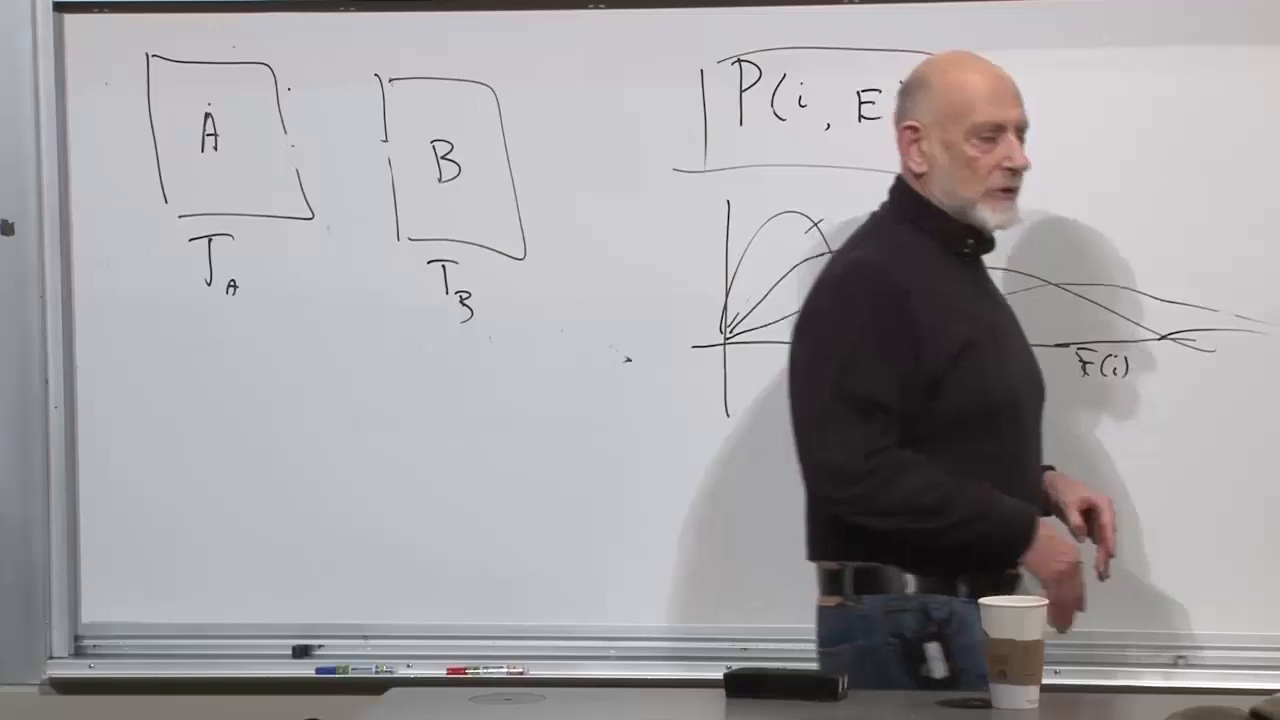
\includegraphics[width=0.88\textwidth]{lecture_02_figure_05.png}
\caption{別々に用意された系\(A\)と\(B\)は、温度\(T_A\)と\(T_B\)でラベル付けされ、弱い熱接触を考える直前の状態にある。}
\lectureframe{00:48:55}
\end{figure}

\begin{figure}[t]
\centering
\begin{tikzpicture}[>=Stealth]
\draw[rounded corners,thick,fill=blue!6] (0,0) rectangle (2.6,2.4);
\draw[rounded corners,thick,fill=orange!8] (5.4,0) rectangle (8,2.4);
\draw[thick] (2.6,1.35) -- (5.4,1.35);
\draw[thick] (2.6,1.05) -- (5.4,1.05);
\draw[<->,very thick] (3.15,1.2) -- (4.85,1.2)
  node[midway,above] {\(\delta E\)};
\node at (1.3,1.45) {\Large \(A\)};
\node at (6.7,1.45) {\Large \(B\)};
\node at (1.3,0.65) {\(T_A,S_A,E_A\)};
\node at (6.7,0.65) {\(T_B,S_B,E_B\)};
\node at (4,0.35) {\small weak thermal contact};
\end{tikzpicture}
\caption{複合系が孤立したままで、エネルギーが弱い接触を通じて揺らぐ。}
\end{figure}

一般性を失うことなく、
\begin{equation}
 T_B>T_A.
 \label{eq:sm2-temperature-order}
\end{equation}
と仮定する。経験によれば、\(B\)がエネルギーを失い、\(A\)がそれを得るはずである。三つの事実が、その予想を計算へと変える。

\subsection{エントロピーの加法性}

微視的な選択肢が独立に組み合わさる二つの弱く結合した部分系に対して、結合した可能性の数は掛け合わされる：
\[
 W_{AB}=W_AW_B.
\]
エントロピーは対数であるから、
\begin{equation}
 S_{\mathrm{tot}}=S_A+S_B.
 \label{eq:sm2-entropy-additivity}
\end{equation}
同じ結果は、積分布のシャノンエントロピーから直接導かれる。

\begin{classroomqa}
\classquestion{なぜ複合系のエントロピーは加算されるのか。}
\lecturerresponse{基礎となる選択肢の数が掛け合わされる一方で、エントロピーは対数をとるからである：
\(\log(W_AW_B)=\log W_A+\log W_B\)。弱い相互作用こそが、部分系の記述とこの主要な加法的形を可能にする。
\lecturetimestamp{00:51:06--00:52:03}}
\end{classroomqa}

\subsection{第一法則と第二法則}

合成系は孤立系であるから、内部で交換されるエネルギーは保存される：
\begin{equation}
 dE_A+dE_B=0,
 \qquad
 dE_B=-dE_A.
 \label{eq:sm2-first-law}
\end{equation}
これが本実験における第一法則である。

ここでは第二法則を公理として受け入れ、そのより深い説明は後に行う。
連結された系が新しい平衡へ緩和するとき、
\begin{equation}
 dS_{\mathrm{tot}}=dS_A+dS_B\geq0.
 \label{eq:sm2-second-law}
\end{equation}
厳密な不等号は平衡から離れた自発的緩和を表し、
等号は可逆な一次変分に対して平衡で成り立つ。

最後に、温度の定義は各々の部分系に適用される：
\begin{equation}
 dE_A=T_A\,dS_A,
 \qquad
 dE_B=T_B\,dS_B.
 \label{eq:sm2-two-temperatures}
\end{equation}

\begin{figure}[H]
\centering
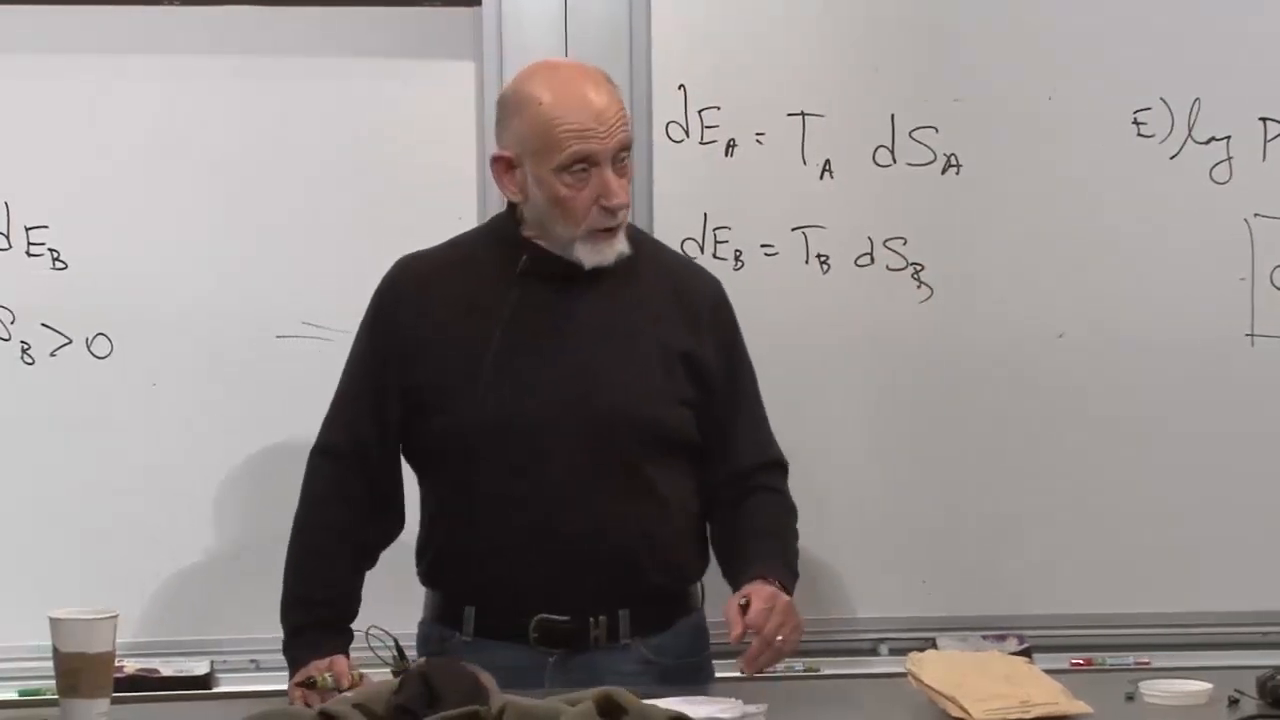
\includegraphics[width=0.88\textwidth]{lecture_02_figure_06.png}
\caption{黒板での議論の最後に現れた二つの部分系の関係
\(dE_A=T_A\,dS_A\) と \(dE_B=T_B\,dS_B\)。}
\lectureframe{00:54:00}
\end{figure}

\subsection{エネルギー流の符号}

これらの式はすでに正味の移動の向きを定めている。
\(dS_A=dE_A/T_A\)、\(dS_B=dE_B/T_B\)、および
\eqref{eq:sm2-first-law} を \eqref{eq:sm2-second-law} に代入すると：
\begin{align}
 dS_{\mathrm{tot}}
 &=\frac{dE_A}{T_A}+\frac{dE_B}{T_B}\\
 &=dE_A\left(\frac{1}{T_A}-\frac{1}{T_B}\right)\geq0.
 \label{eq:sm2-flow-sign}
\end{align}
もし \(T_B>T_A>0\) ならば、
\[
 \frac{1}{T_A}-\frac{1}{T_B}>0.
\]
したがって式 \eqref{eq:sm2-flow-sign} は
\[
 dE_A>0,
 \qquad
 dE_B<0.
\]
を要求する。
低温の系 \(A\) はエネルギーを得て、高温の系 \(B\) はそれを失う。
\(T_A=T_B\) のとき、一次のエントロピー変化は優先される向きを与えず、微視的な交換は釣り合って正味の流れはゼロになる。こうして、
抽象的な導関数 \(T=dE/dS\) は、高温と低温の操作的区別を再現する。

\chapter{多重度、エントロピー、制約付き平衡}

\lectureoverview{確率分布は、その状態がエネルギーを持つと、熱力学的対象となる。まずエントロピーの増大を平衡化と結びつけ、\(dE=T\,dS\)を用いて熱の流れる向きを導く。次に一つの系を多数のレプリカの集まりに置き換え、各占有数の組に対応する配置を数え上げ、この多重度の対数がエントロピーの\(N\)倍であることを示す。したがって平衡は制約付き最大エントロピー問題である。ラグランジュ乗数がそれを解くための方法を与える。}

\section{三つの基本量}

\(i\)が系に許される離散状態を表すものとする。今のところ、離散性は相空間の測度を導入することなく状態を数えられるので有用である。状態\(i\)の確率が\(P_i\)ならば、
\begin{equation}
 \sum_i P_i=1.
 \label{eq:sm3-normalization}
\end{equation}
その状態のエネルギーが\(E_i\)ならば、平均エネルギーは
\begin{equation}
 \overline E=\sum_iP_iE_i.
 \label{eq:sm3-mean-energy}
\end{equation}
\emph{平均}という語が重要である。系が一つの微視的状態において値\(\overline E\)を持つ必要はない。それは可能な値にわたる確率で重み付けした平均である。

\begin{classroomqa}
\classquestion{ここで確率と統計の間に有用な区別はあるか。}
\lecturerresponse{確率は可能な結果の模型を与えるが、統計は通常、観測データから出発し、そこから何が推論できるかを問う。本計算では確率分布を用いるが、同じ平均が統計データにも自然に現れる。授業での非公式なやり取りでは、その区別が続く物理に影響しないため、これらの語は軽く扱われる。
\lecturetimestamp{00:01:39--00:02:21}}
\end{classroomqa}

この分布のエントロピーは
\begin{equation}
 S[P]=-\sum_iP_i\log P_i.
 \label{eq:sm3-entropy}
\end{equation}
この表式は非負である。すべての非零確率は\(0<P_i\leq1\)を満たすので、\(\log P_i\leq0\)であり、\(P_i\to0\)のとき従来の極限値\(P_i\log P_i\to0\)が成り立つ。

\begin{figure}[t]
\centering
\includegraphics[width=0.88\textwidth]{lecture_03_figure_02.png}
\caption{冒頭の板書は、エントロピー、規格化、平均エネルギーの式を、平衡分布の定性的な族とともにまとめている。}
\lectureframe{00:06:44}
\end{figure}

\section{平衡分布の族}

前回の講義は、平衡分布の一パラメータ族を残した。その族を温度でラベル付けしてもよいが、今は平均エネルギー\(\overline E\)でラベル付けする方が有用である。最低可能エネルギーでは、分布は基底状態に集中する。
\[
 P_i=\delta_{i0}.
\]
そのとき状態についての不確かさはなく、\(S=0\)である。平衡分布がより多くのエネルギー準位に広がるにつれて、その平均エネルギーとエントロピーの両方が増大する。

これは熱的な族についての主張であり、考案されうるすべての分布についての主張ではない。任意の族は、より狭くなりながらより大きなエネルギーへ移ることもありうる。導出される平衡分布は、通常の正温度領域ではそのようには振る舞わない。その族に沿って、
\begin{equation}
 \frac{dS}{d\overline E}>0.
 \label{eq:sm3-positive-temperature-branch}
\end{equation}
有界なスペクトルを持つ系は、この導関数が負となる枝を持つこともある。それらの負温度領域は実在するが、本議論では脇に置かれる。

熱平衡は微視的な静止以上のものを意味する。分子は動き、衝突し、エネルギーを交換し続ける。定常になったのは巨視的記述である。分布はもはや正味のドリフトを示さず、系の離れた部分はもはや正味のエネルギー流を支えない。

\section{統計の言葉で表した熱力学法則}

第一法則はエネルギー保存である。第二法則は、孤立した巨視的系の熱力学的エントロピーは減少しないというものである。
\begin{equation}
 \Delta S_{\mathrm{tot}}\geq0.
 \label{eq:sm3-second-law}
\end{equation}
等号は平衡または理想的な可逆変化を表し、自発的な緩和は通常、厳密な増大を与える。

確率的な描像では、緩和は、我々が依然として区別する巨視的な選択肢の上に重みを広げる傾向がある。この主張には講義で強調された限定が必要である。我々は\emph{粗視化}しているのである。厳密なハミルトニアン発展は細視化された相空間エントロピーを保存する。巨視的エントロピーが増大するのは、我々が微視的な相関と詳細を追跡するのをやめるからである。そのような情報を失うことは、縮約された記述を広げる。自発的な狭まりは、代わりに、測定を行うことなく微視的情報を得たことを意味するであろう。

第零法則は、系が熱平衡に達しうること、そして平衡が推移的であることを主張する。\(A\) が \(B\) と平衡にあり、\(B\) が \(C\) と平衡にあるならば、\(A\) は \(C\) と平衡にある。温度は、この推移性を明白にする数を与える：
\[
 T_A=T_B,\qquad T_B=T_C
 \quad\Longrightarrow\quad
 T_A=T_C.
\]
平衡にないとき、エネルギーは温度のより大きい部分系から温度のより小さい部分系へ流れる。温度が等しいとき、正味の流れは止む。次に、この操作的命題を温度のエントロピー定義から導く。

\section{なぜエネルギーは高温から低温へ流れるのか}

弱く結合した二つの部分系 \(A\) と \(B\) を考える。それぞれは内部的に平衡にあるが、それらの温度は異なる。ラベルを
\begin{equation}
 T_B>T_A>0.
 \label{eq:sm3-temperature-order}
\end{equation}
となるように選ぶ。小さな交換の間、合成エネルギーの保存により
\begin{equation}
 dE_A+dE_B=0.
 \label{eq:sm3-energy-conservation}
\end{equation}
が成り立つ。第2法則により
\begin{equation}
 dS_A+dS_B\geq0.
 \label{eq:sm3-entropy-change}
\end{equation}
が成り立つ。内部的に平衡にある各部分系について、温度は
\begin{equation}
 dE_X=T_X\,dS_X,
 \qquad X=A,B.
 \label{eq:sm3-temperature-differential}
\end{equation}
によって定義される。これを \eqref{eq:sm3-energy-conservation} に代入すると
\begin{equation}
 T_A\,dS_A+T_B\,dS_B=0,
\end{equation}
が得られ、したがって
\begin{equation}
 dS_B=-\frac{T_A}{T_B}\,dS_A.
 \label{eq:sm3-dsb}
\end{equation}
となる。この結果を \eqref{eq:sm3-entropy-change} に入れると、
\begin{align}
 dS_{\mathrm{tot}}
 &=dS_A-\frac{T_A}{T_B}dS_A\\
 &=\frac{T_B-T_A}{T_B}\,dS_A\geq0.
 \label{eq:sm3-flow-entropy}
\end{align}
となる。\(T_B-T_A>0\) かつ \(T_B>0\) であるから、自発的な交換には
\[
 dS_A>0.
\]
が必要である。すると式 \eqref{eq:sm3-temperature-differential} により
\begin{equation}
 dE_A=T_A\,dS_A>0,
 \qquad
 dE_B=-dE_A<0.
 \label{eq:sm3-hot-to-cold}
\end{equation}
が得られる。エネルギーは、より高温の部分系である \(B\) から、より低温の \(A\) へ流れた。ここで熱とは、単に移動中のエネルギーである。流れは \(T_A=T_B\) となるまで続き、そのとき一次のエントロピー変化はもはやどちらの向きも有利にしない。

同じ結果は一行で表示できる：
\begin{equation}
 dS_{\mathrm{tot}}
 =dE_A\left(\frac{1}{T_A}-\frac{1}{T_B}\right)\geq0.
 \label{eq:sm3-compact-flow}
\end{equation}
逆温度差の符号が \(dE_A\) の符号を定める。この簡潔な形は、後に正準集団と自然に適合するであろう。

\begin{classroomqa}
\audiencequestion{この議論は、\(A\) と \(B\) がそれぞれすでに内部平衡にあることを仮定しているのか。}
\lecturerresponse{はい。単一の \(T_A\) または \(T_B\) を割り当てることは、その仮定を置くことである。部分系が内部的に平衡でないなら、それをより小さな領域に分割し、温度を定義できるところで局所的にこの議論を適用する。そのとき大域的な緩和は、それらの領域間の交換から組み立てられる。
\lecturetimestamp{00:24:38--00:25:22}}
\end{classroomqa}

\section{何が状態と数えられるのか}

平衡確率を問う前に、ラベル \(i\) が何を意味するのかを知らなければならない。微視的状態とは、基礎となる物理法則によって許される、系の最も完全な指定である。古典力学では、すべての粒子の位置と運動量を思い描く。量子力学では、状態は代わりに完全な量子状態であり、不確定性原理はすべての古典的な位置と運動量を同時に鋭く指定することを妨げる。

有限の箱の中の量子系では、関連する状態の数え上げは離散的でありうる。古典統計力学は適切な極限で現れ、そこでは密に間隔を置いた量子状態にわたる和が相空間積分になる。その極限操作はまた、連続的なエントロピーを無次元にするために必要な相空間セルを導入する。それは単に和の記号を積分の記号に置き換えることによって得られるのではない。

\begin{classroomqa}
\audiencequestion{気体について、状態はすべての分子の位置と運動量として思い描くべきなのか。}
\lecturerresponse{それが正しい古典的描像である。より一般には、状態とは、物理法則に従う限りで原理的に知りうるすべてを意味する。量子力学はその最大限の記述の形を変え、有限体積での数え上げを離散的にする。量子和から古典積分を回復することは、真の極限議論であり、一行の置き換えではない。
\lecturetimestamp{00:25:31--00:27:38}}
\end{classroomqa}

\section{レプリカからなる熱浴}

難しい問いは今や避けられない：平衡が確立した後、何が \(P_i\) を決めるのか。

部分系を非常に大きな熱浴と接触させる。エネルギーは行き来してよいが、熱浴はあまりに多くの自由度をもつため、少量のエネルギーの移動はその温度をほとんど変えない。特に便利な熱浴は、部分系自身の弱く結合した多数のレプリカからなる。一つのレプリカが研究対象の系であり、他のレプリカがその環境を構成する。

この構成はしばしば現実の巨視的系を映し出す。大きなほぼ均質な物体を多数の類似したセルに分割する。各セルは部分系であり、残りのセルがその熱浴として働く。レプリカの総数を \(N\) で表す。教室でのデモンストレーションは9個のレプリカと3つの色付き状態ラベルを用いるが、数え上げはそれらの特定の数に依存しない。

\(n_i\) を状態 \(i\) にあるレプリカの数とする。これらは \emph{占有数} である。可能なエネルギー準位は無限に多くありうるが、有限の全エネルギーでは、非常に高い準位のほとんどは無視できるかゼロの占有をもつ。

第一の制約は単にレプリカの数である：
\begin{equation}
 \sum_i n_i=N.
 \label{eq:sm3-number-constraint}
\end{equation}
第二は全エネルギーである：
\begin{equation}
 \sum_i n_iE_i=N\overline E.
 \label{eq:sm3-total-energy-constraint}
\end{equation}
右辺は示量的である。レプリカの数を2倍にし、その統計的状態を固定したままにすれば、全エネルギーは2倍になるが、レプリカ1個あたりの平均エネルギーは\(\overline E\)のままである。

\begin{classroomqa}
\audiencequestion{レプリカ構成はエネルギー制約も満たさなければならないか。}
\lecturerresponse{はい。占有数は\(N\)に加算されなければならず、そのエネルギー重み付き和は固定された全エネルギー\(N\overline E\)に等しくなければならない。これらはまさに、後にエントロピー最大値を制限することになる二つの制約である。
\lecturetimestamp{00:37:12--00:39:54}}
\end{classroomqa}

無作為に選ばれたレプリカが状態\(i\)を占める確率は、その相対頻度である：
\begin{equation}
 P_i=\frac{n_i}{N},
 \qquad
 n_i=NP_i.
 \label{eq:sm3-frequency-probability}
\end{equation}

\begin{figure}[t]
\centering
\includegraphics[width=0.82\textwidth]{lecture_03_figure_03.png}
\caption{エネルギー準位の描像と、確率を占有分率\(P_i=n_i/N\)と同一視すること。}
\lectureframe{00:41:40}
\end{figure}

\begin{classroomqa}
\audiencequestion{黒板にある\(N(i)\)という記法は\(n_i\)と異なる意味を意図しているのか。}
\lecturerresponse{いいえ。どちらも状態\(i\)の占有数を表す。我々は\(n_i\)を一貫して用い、大文字の\(N\)はレプリカの総数に取ってある。
\lecturetimestamp{00:41:28--00:41:33}}
\end{classroomqa}

\eqref{eq:sm3-number-constraint}と\eqref{eq:sm3-total-energy-constraint}を\(N\)で割ると、確率の制約が再現される：
\begin{equation}
 \sum_iP_i=1,
 \qquad
 \sum_iP_iE_i=\overline E.
 \label{eq:sm3-probability-constraints}
\end{equation}
したがって、アンサンブル頻度の解釈は、我々が出発点とした方程式を再現した。

\section{占有パターンの多重度}

占有数の組\(\{n_i\}\)を固定する。\(N\)個の区別可能なレプリカを状態に割り当てて、ちょうどその組を実現する方法は何通りあるか。答えは多項係数
\begin{equation}
 C(\{n_i\})=\frac{N!}{\prod_i n_i!}.
 \label{eq:sm3-multiplicity}
\end{equation}
である。分母を見るには、まず\(N\)個のラベル付きレプリカを\(N!\)通りに並べる。同じ状態を占める\(n_i\)個のレプリカを入れ替えても新しい占有の割り当ては生じないので、各状態について\(n_i!\)で割る。

\begin{figure}[t]
\centering
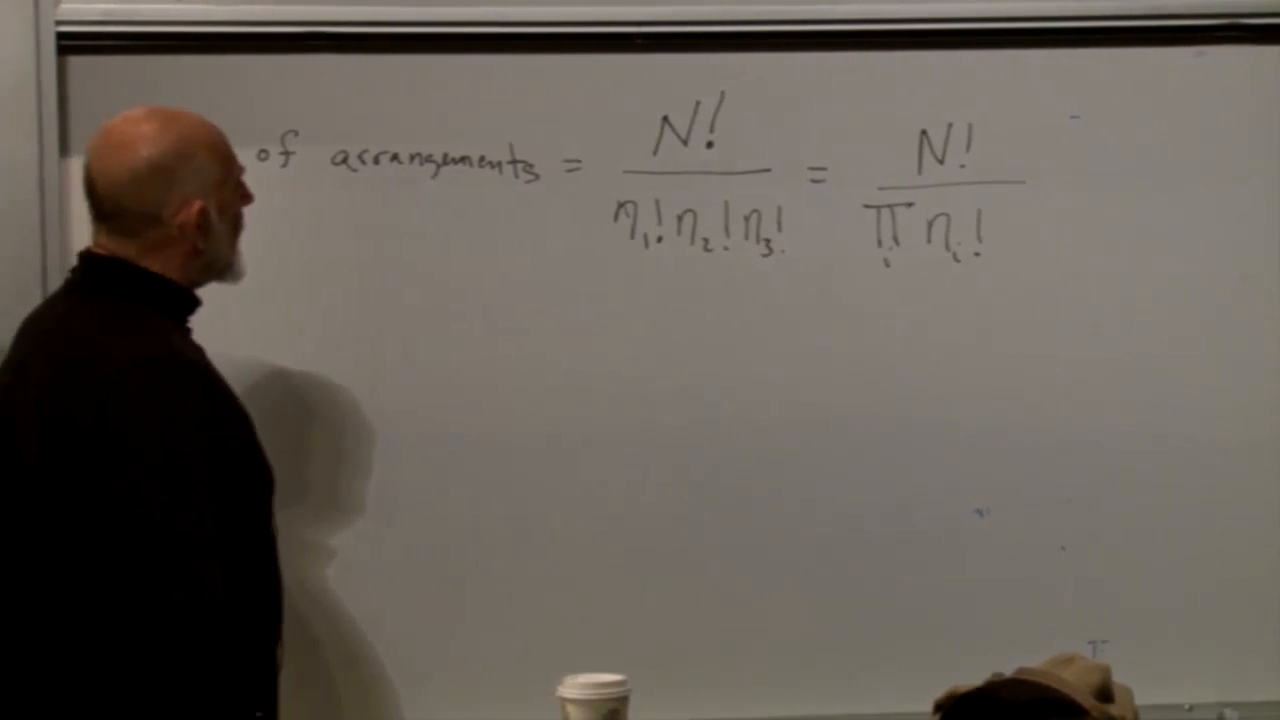
\includegraphics[width=0.88\textwidth]{lecture_03_figure_04.png}
\caption{黒板に書かれた多項係数の多重度\(C=N!/\prod_i n_i!\)。}
\lectureframe{00:46:55}
\end{figure}

占有されていない準位は\(0!=1\)であるから問題を生じない。すべてのレプリカが一つの状態を占めるならば、予想どおり
\[
 C=\frac{N!}{N!}=1,
\]
となる。3個のレプリカが指定された3つの異なる状態を占めるならば、
\[
 C=\frac{3!}{1!\,1!\,1!}=6.
\]
である。2個のレプリカが指定された2つの状態を占める場合、この式は2通りの割り当てを与える：どのラベル付きレプリカがどちらの状態を占めるかを交換するのである。

\begin{classroomqa}
\audiencequestion{二つの制約を満たす占有数の組は複数あり得るか。}
\lecturerresponse{通常は多数ある。式\eqref{eq:sm3-multiplicity}はまず一つの固定された組\(\{n_i\}\)に対する配置を数えるだけで、それが制約を満たすかどうかはまだ決めていない。次の段階では、制約に適合するすべての組を比較し、どれが最大の多重度をもつかを見出す。
\lecturetimestamp{00:48:07--00:48:43}}
\end{classroomqa}

統計的仮定とは、孤立した設定と両立する微視的割り当てを対称に扱うことである。したがって、より多くの割り当てによって実現される巨視的占有パターンの方がより確からしい。大きな\(N\)に対して、分率\(n_i/N\)の上の分布は鋭く尖る。平衡分率は、\eqref{eq:sm3-number-constraint}と\eqref{eq:sm3-total-energy-constraint}を条件として\(C\)を最大化する値である。

\section{スターリングの近似}

階乗は\(N\)が巨視的な値に達するはるか前に巨大になるので、我々はその対数を扱う。まず
\begin{equation}
 \log N!=\sum_{x=1}^{N}\log x.
 \label{eq:sm3-log-factorial-sum}
\end{equation}
から始める。大きな\(N\)に対して、和は\(\log x\)の下の面積で近似される：
\begin{align}
 \log N!
 &\simeq\int_1^N\log x\,dx\\
 &=\left[x\log x-x\right]_1^N\\
 &=N\log N-N+1.
 \label{eq:sm3-stirling-integral}
\end{align}
原始関数は
\[
 \frac{d}{dx}(x\log x-x)=\log x.
\]
から直ちに従う。主要な示量的次数では、加法的定数は落としてよい：
\begin{equation}
 \log N!\simeq N\log N-N.
 \label{eq:sm3-stirling-log}
\end{equation}
指数をとると、講義で用いられた簡略形
\begin{equation}
 N!\simeq N^N e^{-N}.
 \label{eq:sm3-stirling-simple}
\end{equation}
が得られる。

\begin{figure}[t]
\centering
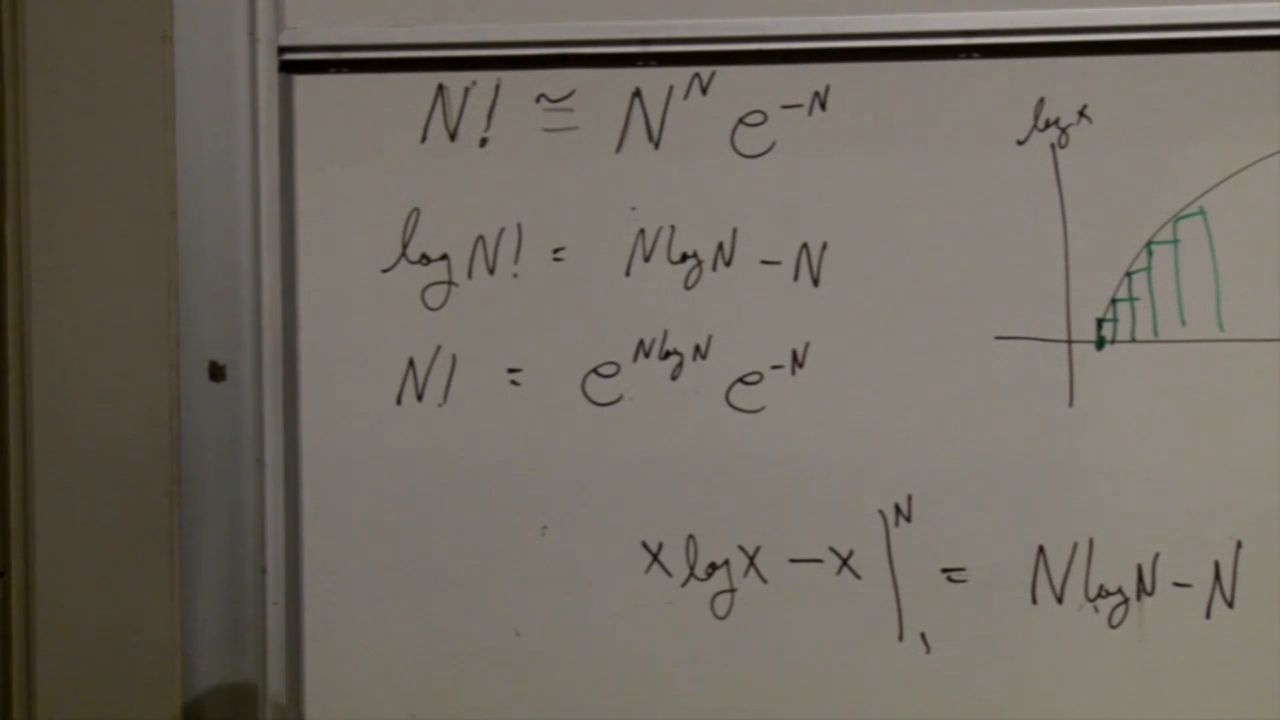
\includegraphics[width=0.88\textwidth]{lecture_03_figure_05.png}
\caption{主要なスターリング近似と、\(\log x\)の和を積分で置き換えることによるその導出。}
\lectureframe{01:03:45}
\end{figure}

\begin{classroomqa}
\audiencequestion{\(x\log x-x\)を下限で評価すると余分な\(+1\)が残るか。}
\lecturerresponse{はい。式\eqref{eq:sm3-stirling-integral}はその定数を含む。\(N\to\infty\)のとき、それは\(N\)に比例する項に比べて無視できる。だから主要な式ではそれを省く。和自体は\(x=1\)から始めなければならない。\(\log0\)は定義されない。
\lecturetimestamp{01:04:12--01:04:35}}
\end{classroomqa}

\begin{classroomqa}
\audiencequestion{\(\sqrt{N}\)に比例する因子も欠けているか。}
\lecturerresponse{はい。より精密な漸近式は
\[
 N!\sim\sqrt{2\pi N}\left(\frac{N}{e}\right)^N.
\]
である。その対数は\(\tfrac12\log(2\pi N)\)だけを加えるが、これは\(N\log N-N\)に比べて非示量的である。それは正確な有限\(N\)の確率には重要だが、巨視的系の主要なエントロピー計算には重要でない。
\lecturetimestamp{01:04:35--01:05:40}}
\end{classroomqa}

スターリングの近似は、\eqref{eq:sm3-multiplicity} の分母においても注意して用いなければならない。熱力学的極限では、ゼロでない極限確率をもつ状態は \(n_i=NP_i\) を満たすので、その占有数は \(N\) とともに増大する。占有数がごく小さいか消えてしまう状態は、有限のエネルギー遮断で扱い、その後で極限をとることによって復元できる。主要な示量的エントロピーは、省略された次次の項によって影響を受けない。

\section{多重度の対数はエントロピーである}

\eqref{eq:sm3-stirling-simple} を分子および巨視的に占有されたすべての分母因子に適用する：
\begin{equation}
 C\simeq
 \frac{N^Ne^{-N}}
 {\prod_i n_i^{\,n_i}e^{-n_i}}.
 \label{eq:sm3-c-stirling}
\end{equation}
\(\sum_i n_i=N\) であるから、主要な指数因子は相殺する：
\begin{equation}
 C\simeq\frac{N^N}{\prod_i n_i^{\,n_i}}.
 \label{eq:sm3-c-leading}
\end{equation}
積よりも対数のほうが最大化しやすく、また対数は単調であるから、両方の極大は同じ占有パターンで起こる：
\begin{equation}
 \log C=N\log N-\sum_i n_i\log n_i.
 \label{eq:sm3-logc-occupations}
\end{equation}
ここで \(n_i=NP_i\) を代入する：
\begin{align}
 \log C
 &=N\log N-\sum_iNP_i\log(NP_i)\\
 &=N\log N-N\sum_iP_i\log N
   -N\sum_iP_i\log P_i\\
 &=-N\sum_iP_i\log P_i,
 \label{eq:sm3-logc-entropy-derivation}
\end{align}
ここで規格化により二つの \(N\log N\) の項が相殺される。したがって、\(N\) の主要な次数まで、
\begin{equation}
 \boxed{\log C=NS}.
 \label{eq:sm3-logc-ns}
\end{equation}

\begin{figure}[t]
\centering
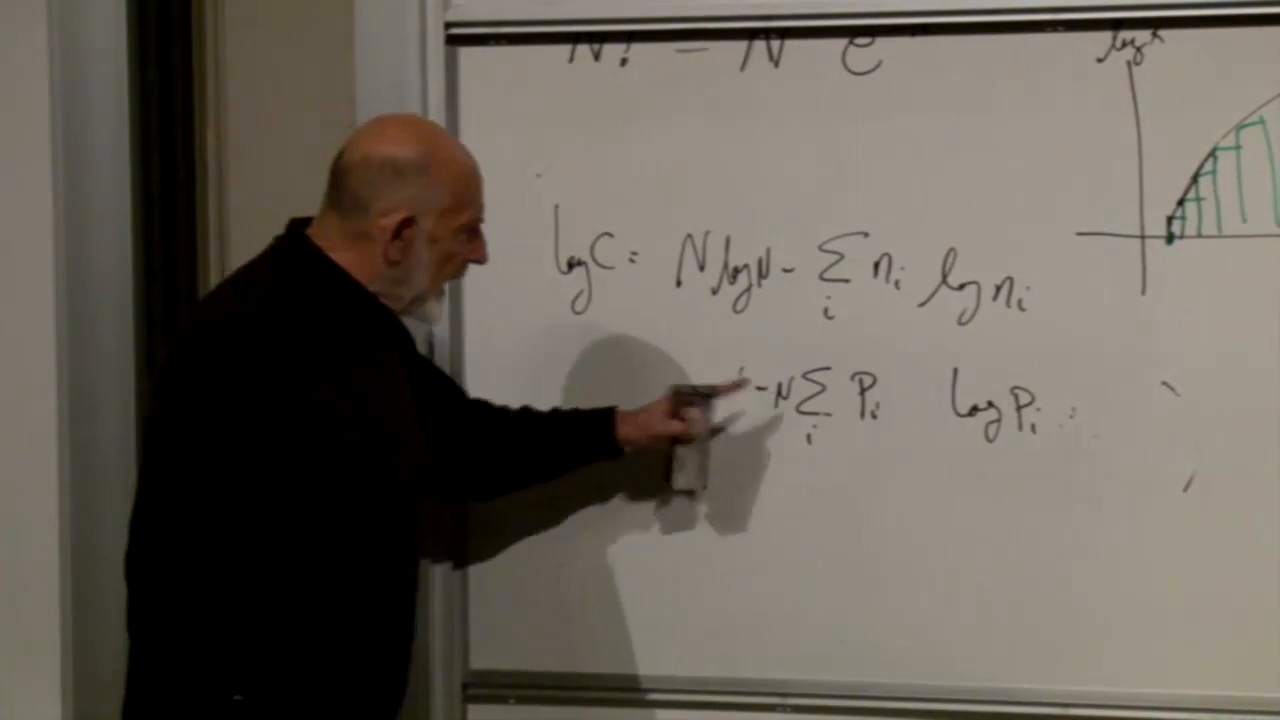
\includegraphics[width=0.88\textwidth]{lecture_03_figure_06.png}
\caption{\(\log C=N\log N-\sum_i n_i\log n_i\) を
\(-N\sum_iP_i\log P_i=NS\) に結びつける板書の計算。}
\lectureframe{01:16:10}
\end{figure}

この関係はこの章の概念的中心である。エントロピーは、数え上げ問題に押しつけられた無関係な量ではない。それは、対数的に測られた、一つのレプリカあたりの多重度である。したがって、微視的配置の数を最大化することは、主要な次数において、一つのレプリカのエントロピーを最大化することと同一である。

\begin{classroomqa}
\audiencequestion{すべての占有数が等しいときに多重度が最大になるのではないか。}
\lecturerresponse{どの状態も区別されず、有限個の状態にわたって \(\sum_i n_i=N\) だけが課されているときには一様である。固定エネルギーの拘束は、値 \(E_i\) が異なるために答えを変える。等しい占有は一般に、指定された平均エネルギーを生み出さない。
\lecturetimestamp{01:17:07--01:18:20}}
\end{classroomqa}

\begin{classroomqa}
\audiencequestion{大文字の \(N\) は大きいが、なぜスターリングの近似を分母のすべての \(n_i\) に適用してよいのか。}
\lecturerresponse{ゼロでない極限確率をもつ各状態について、\(n_i=NP_i\) は \(N\) に比例して増大する。まず有限のエネルギー範囲を保ち、そこで大きな \(N\) の極限をとり、その後で範囲を広げればよい。まばらな裾の状態には別個の有限補正が必要であるが、それらは主要な示量的エントロピーを変えない。
\lecturetimestamp{01:18:23--01:19:28}}
\end{classroomqa}

\begin{classroomqa}
\audiencequestion{この大きな \(N\) の近似が、以前に粗視化によって意味されていたものか。}
\lecturerresponse{いいえ。熱力学的極限は、大きな占有数と漸近的な数え上げを制御する。粗視化は、微視的分解能の喪失または意図的な破棄である。両者はしばしば巨視的統計力学でともに用いられるが、別個の操作である。
\lecturetimestamp{01:19:29--01:19:46}}
\end{classroomqa}

\begin{classroomqa}
\audiencequestion{
\(\log C=N\log N-\sum_i n_i\log n_i\) であるから、第二項は最大化ではなく最小化されるべきではないか。}
\lecturerresponse{はい。\(N\) を固定すると、\(\log C\) を最大化することは \(\sum_i n_i\log n_i\) を最小化することと等価である。\(n_i=NP_i\) を代入した後、固定された \(N\log N\) の項は相殺し、残るのは
\(-N\sum_iP_i\log P_i=NS\) である。したがって、同じ操作は、正のエントロピー \(S\) を最大化することとしてより自然に記述される。
\lecturetimestamp{01:19:48--01:20:55}}
\end{classroomqa}

\begin{classroomqa}
\audiencequestion{なぜ対称性によって直ちに議論を終え、すべての \(n_i\) を等しいと置かないのか。}
\lecturerresponse{その近道はエネルギーのラベルを無視している。規格化の拘束は状態を対称に扱うが、
\(\sum_iP_iE_i=\overline E\) はそうではない。異なるエネルギーの状態は異なる寄与をする。エネルギー拘束こそが、一様でない平衡分布が入ってくるまさにその場所である。
\lecturetimestamp{01:21:15--01:21:41}}
\end{classroomqa}

\section{最大エントロピー問題}

これで統計力学的規則を曖昧さなく述べることができる。確率 \(P_i\) を変化させて、
\begin{equation}
 S[P]=-\sum_iP_i\log P_i
 \label{eq:sm3-maximize-entropy}
\end{equation}
を
\begin{equation}
 \sum_iP_i=1,
 \qquad
 \sum_iP_iE_i=\overline E.
 \label{eq:sm3-maxent-constraints}
\end{equation}
の下で最大化する。最大化する確率は、大きなレプリカ集団の鋭く優先される占有分率を与える。占有数は揺らぐが、その相対的ずれは \(N\) が増大するにつれて縮小するので、比 \(n_i/N\) はよく定義された熱力学的確率となる。

\begin{classroomqa}
\audiencequestion{\(E_i\) は固定された状態エネルギーであり、拘束は別に与えられた全エネルギーを用いるのか。}
\lecturerresponse{はい。スペクトル \(\{E_i\}\) は部分系に属する。完全なレプリカの集まりは固定された全エネルギーをもつが、エネルギーは絶えずレプリカ間を移動する。その全エネルギーを \(N\) で割ることは、一つのレプリカの平均エネルギー \(\overline E\) を固定するのであり、各微視的実現におけるそのエネルギーを固定するのではない。
\lecturetimestamp{01:26:12--01:27:07}}
\end{classroomqa}

問題を述べるのは容易だが、まだ解かれてはいない。二つの拘束をもつ極値化であるから、もう一つの数学的道具が必要である。

\section{ラグランジュ乗数}

制約のない関数 \(F(x_1,x_2,\ldots)\) に対して、停留点は
\begin{equation}
 \frac{\partial F}{\partial x_i}=0
 \qquad\text{for every }i.
 \label{eq:sm3-unconstrained-stationary}
\end{equation}
を満たす。
ここでさらに
\begin{equation}
 G(x_1,x_2,\ldots)=0.
 \label{eq:sm3-one-constraint}
\end{equation}
を要求する。

\begin{classroomqa}
\audiencequestion{図に座標 \(x\) と \(y\) があるとき、\(x\) とは何を意味するのか。}
\lecturerresponse{ここで \(x\) は座標ベクトル全体
\((x_1,x_2,\ldots)\) の略記である。二次元の図では、その成分は単に \(x\) と \(y\) である。後にその成分は確率
\(P_1,P_2,\ldots\) となる。
\lecturetimestamp{01:30:12--01:30:20}}
\end{classroomqa}

幾何学的には、レベル曲線 \(F=\text{constant}\) は等高線図をなし、
一方 \(G=0\) は系が運動を許される曲線である。制約付き極値は、\(F\) のある等高線が制約曲線に接する場所で生じる。その点で勾配は平行である：
\begin{equation}
 \nabla F=-\lambda\nabla G
 \label{eq:sm3-parallel-gradients}
\end{equation}
ある数 \(\lambda\) に対して。

\begin{figure}[t]
\centering
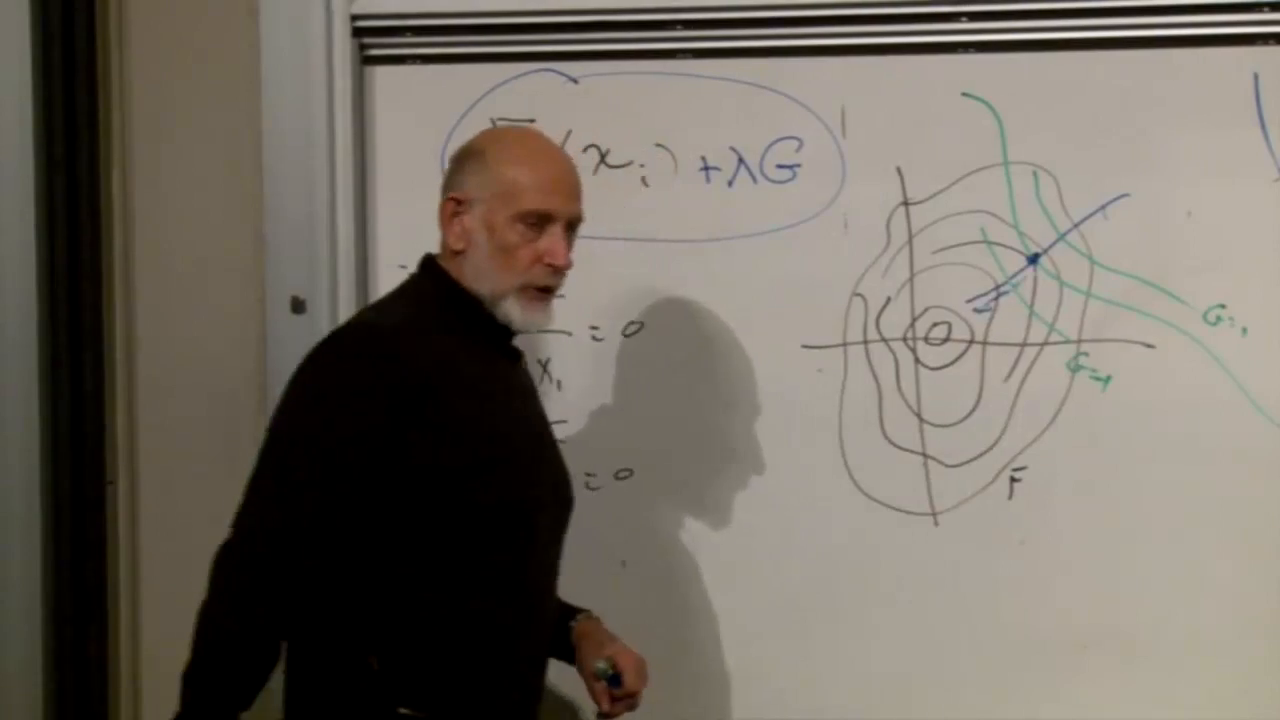
\includegraphics[width=0.88\textwidth]{lecture_03_figure_07.png}
\caption{黒板の等高線幾何と拡張関数
\(F'=F+\lambda G\)。制約付き極値は接点で生じる。}
\lectureframe{01:37:10}
\end{figure}

式 \eqref{eq:sm3-parallel-gradients} は、拡張関数
\begin{equation}
 F'=F+\lambda G
 \label{eq:sm3-augmented-function}
\end{equation}
を定義し、通常の停留性を要求することによって得られる：
\begin{equation}
 \frac{\partial F'}{\partial x_i}=0.
 \label{eq:sm3-augmented-stationarity}
\end{equation}
乗数 \(\lambda\) は最初は未知である。それによって系が不定になるわけではない。なぜなら元の制約 \(G=0\) が追加の方程式を一つ与えるからである。

\begin{classroomqa}
\classquestion{なぜ \(G\) に比例する項を加えると、制約付きの点が停留になるのか。}
\lecturerresponse{制約付き極値では、\(G=0\) に接する方向の運動はすでに \(F\) の一次の変化を生じない。残る傾きは制約に垂直な方向だけである。\(\nabla G\) は同じ垂直方向を向くので、適切な \(\lambda\) がそれを打ち消す：
\(\nabla F+\lambda\nabla G=0\)。
\lecturetimestamp{01:35:06--01:35:32}}
\end{classroomqa}

\section{二変数の例}


\begin{equation}
 F(x,y)=\frac{x^2+y^2}{2}
 \label{eq:sm3-example-f}
\end{equation}
を
\begin{equation}
 x+y=1.
 \label{eq:sm3-example-constraint}
\end{equation}
の下で最小化する。制約を \(G=x+y-1=0\) と書き、
\begin{equation}
 F'=\frac{x^2+y^2}{2}+\lambda(x+y-1).
 \label{eq:sm3-example-augmented}
\end{equation}
を作る。停留方程式は
\begin{align}
 \frac{\partial F'}{\partial x}&=x+\lambda=0,\\
 \frac{\partial F'}{\partial y}&=y+\lambda=0.
 \label{eq:sm3-example-derivatives}
\end{align}
である。したがって \(x=y=-\lambda\)。残る方程式は制約であり、
\[
 x+y=-2\lambda=1,
\]
よって
\begin{equation}
 \lambda=-\frac12,
 \qquad
 x=y=\frac12.
 \label{eq:sm3-example-solution}
\end{equation}
点 \((1/2,1/2)\) は、原点を中心とする最小の円が直線 \(x+y=1\) に接する点である。

\begin{figure}[t]
\centering
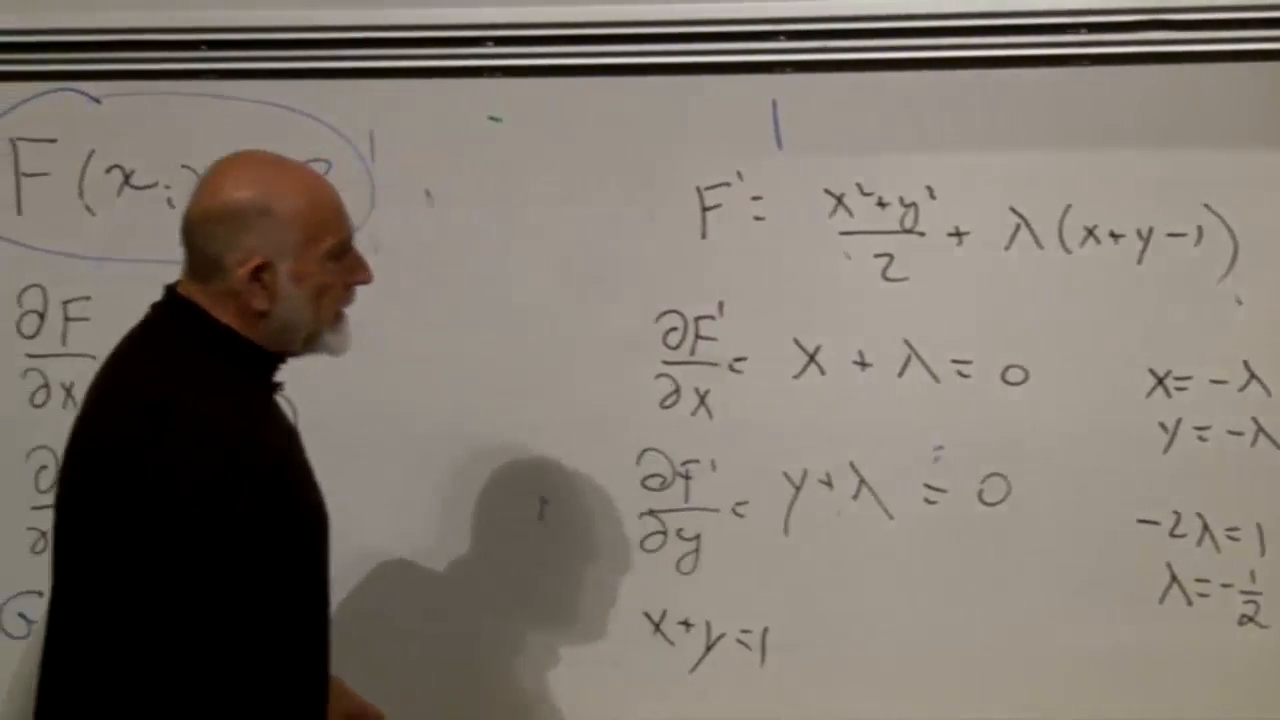
\includegraphics[width=0.88\textwidth]{lecture_03_figure_08.png}
\caption{\(x+y=1\) の下で \((x^2+y^2)/2\) を最小化するための、完成したラグランジュ乗数の計算。}
\lectureframe{01:44:10}
\end{figure}

制約が複数ある場合は、それぞれに一つの乗数を導入する：
\begin{equation}
 F'=F+\lambda_1G_1+\lambda_2G_2+\cdots.
 \label{eq:sm3-many-multipliers}
\end{equation}
次に
\begin{equation}
 \begin{aligned}
 \frac{\partial F'}{\partial x_i}&=0
 &&\text{for every }i,\\
 G_a&=0
 &&\text{for every constraint }a.
 \end{aligned}
 \label{eq:sm3-many-equations}
\end{equation}
を解く。講義では、意図的に人為的な練習問題を提案する：\(x,y,z\) の二次関数を、\(x+y=1\) や \(z+x=1\) のような二つの独立な線形制約を課しながら極値化する。その目的は特定の答えではなく、各制約が一つの乗数と一つの方程式の両方をもたらすという規則である。

\section{次の講義に備えた問題}

統計力学では、座標は確率
\(\{P_i\}\) であり、最大化すべき関数はエントロピーであり、制約は規格化と固定された平均エネルギーである。
\begin{align}
 S[P]&=-\sum_iP_i\log P_i,\\
 G_1[P]&=\sum_iP_i-1,\\
 G_2[P]&=\sum_iP_iE_i-\overline E.
 \label{eq:sm3-final-functions}
\end{align}
を定義する。したがって拡張エントロピーは
\begin{equation}
 \Phi[P]
 =S[P]+\alpha G_1[P]+\beta G_2[P].
 \label{eq:sm3-final-augmented}
\end{equation}
と書ける。解くべき方程式は
\begin{equation}
 \frac{\partial\Phi}{\partial P_i}=0
 \quad\text{for every }i,
 \qquad
 G_1=0,
 \qquad
 G_2=0.
 \label{eq:sm3-final-problem}
\end{equation}

\begin{figure}[H]
\centering
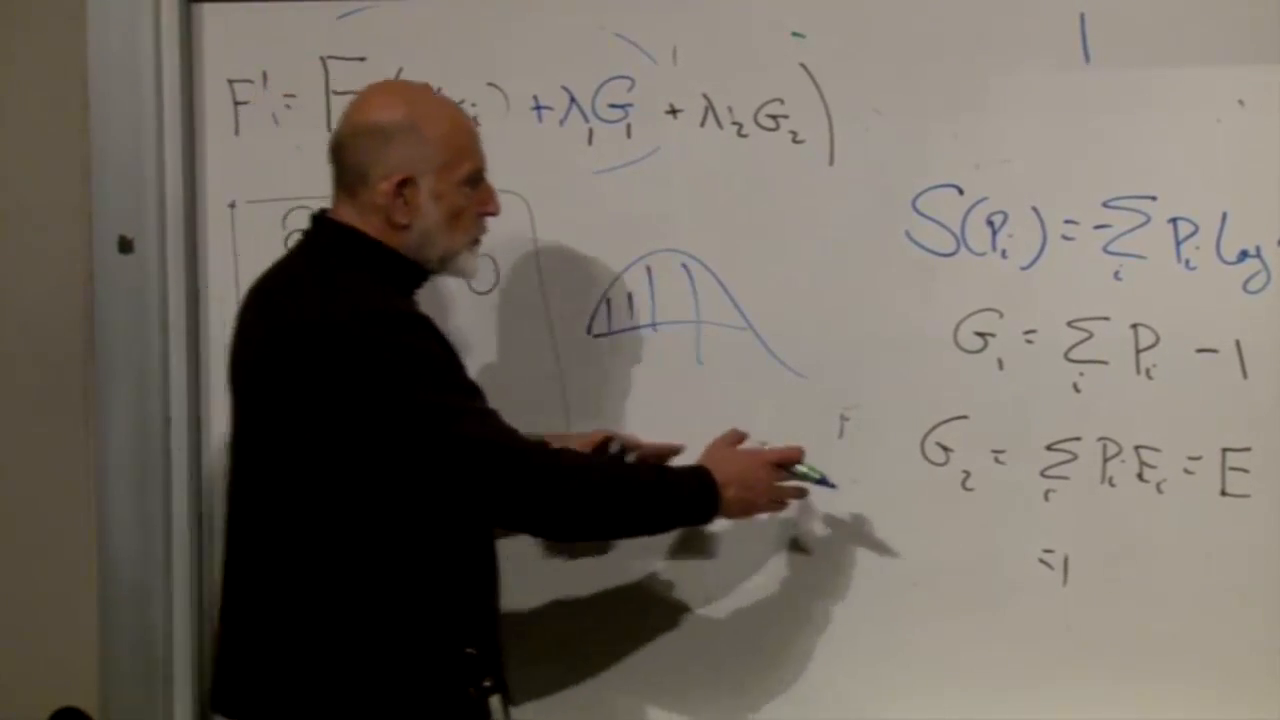
\includegraphics[width=0.88\textwidth]{lecture_03_figure_09.png}
\caption{締めくくりの黒板：確率の関数としてのエントロピー、および規格化と固定された平均エネルギー。}
\lectureframe{01:53:05}
\end{figure}

この時点で問題は完全に定式化された。
\eqref{eq:sm3-final-problem}
を解くと平衡分布が得られる。エネルギーに共役な乗数は、\eqref{eq:sm3-final-augmented} で選ばれた符号の規約を除いて、逆温度
\(\beta=1/T\) となる。次の講義ではその微分を実行し、ボルツマン重みを得る。
\chapter{ボルツマン重み、分配関数、理想気体}

\lectureoverview{正規化と平均エネルギーを固定したもとでエントロピーを最大化することにより、平衡確率分布を導出する。次に分配関数から、微分によって平均エネルギー、エントロピー、温度が得られる。理想気体が最初の完全な例を与え、続いて重力への拡張とエネルギー揺らぎの予告が示される。}

\section{制約付きエントロピー問題}

同じ部分系の同一の、非常に弱く相互作用する\(\mathcal N\)個の複製からなる大きな集団から始める。\(n_i\)個の複製が\(i\)番目の状態を占めるならば、
\begin{equation}
 p_i=\frac{n_i}{\mathcal N},
 \qquad
 \sum_i p_i=1.
 \label{eq:sm4-occupation-probability}
\end{equation}
前回の講義で行った多項係数の数え上げにより、複製あたりのエントロピーは
\begin{equation}
 S[p]=-\sum_i p_i\log p_i.
 \label{eq:sm4-entropy}
\end{equation}
となる。これをすべての変数\(p_1,p_2,\ldots\)の通常の関数とみなすことは有用である。その単純な加法的形が計算を可能にするのである。

複製の集まりは固定された全エネルギー\(\mathcal N E\)をもつ。ここで\(E\)は複製あたりの平均エネルギーである。したがって第二の制約は
\begin{equation}
 \sum_i p_iE_i=E.
 \label{eq:sm4-energy-constraint}
\end{equation}
準位\(E_i\)は部分系に属し、右辺の数\(E\)はそれらの確率重み付き平均である。\eqref{eq:sm4-occupation-probability}および\eqref{eq:sm4-energy-constraint}のもとで\eqref{eq:sm4-entropy}を最大化することにより、圧倒的に最も確からしい占有確率が選び出される。

便宜上、\(-S=\sum_i p_i\log p_i\)を最小化する。各制約に対してラグランジュ乗数を一つ導入する：
\begin{equation}
 \begin{aligned}
 \Phi[p;\alpha,\beta]
 &=\sum_i p_i\log p_i\\
 &\quad+\alpha\left(\sum_i p_i-1\right)\\
 &\quad+\beta\left(\sum_i p_iE_i-E\right).
 \end{aligned}
 \label{eq:sm4-augmented-functional}
\end{equation}
\(\alpha\)および\(\beta\)という名称は、まだ物理的な仮定ではない。この段階では、二つの制約を課すために必要な二つの数にすぎない。

\begin{classroomqa}
\audiencequestion{拡張された関数は\(\alpha\)および\(\beta\)の関数でもあるのか。}
\lecturerresponse{はい。\(\alpha\)および\(\beta\)に関して変分すれば、二つの制約が回復される。しかし当面の計算では、これらの乗数を固定して確率\(p_i\)を変分する。それらの値は後で正規化と指定された平均エネルギーによって固定される。\lecturetimestamp{00:09:32--00:09:49}}
\end{classroomqa}

\begin{figure}[t]
\centering
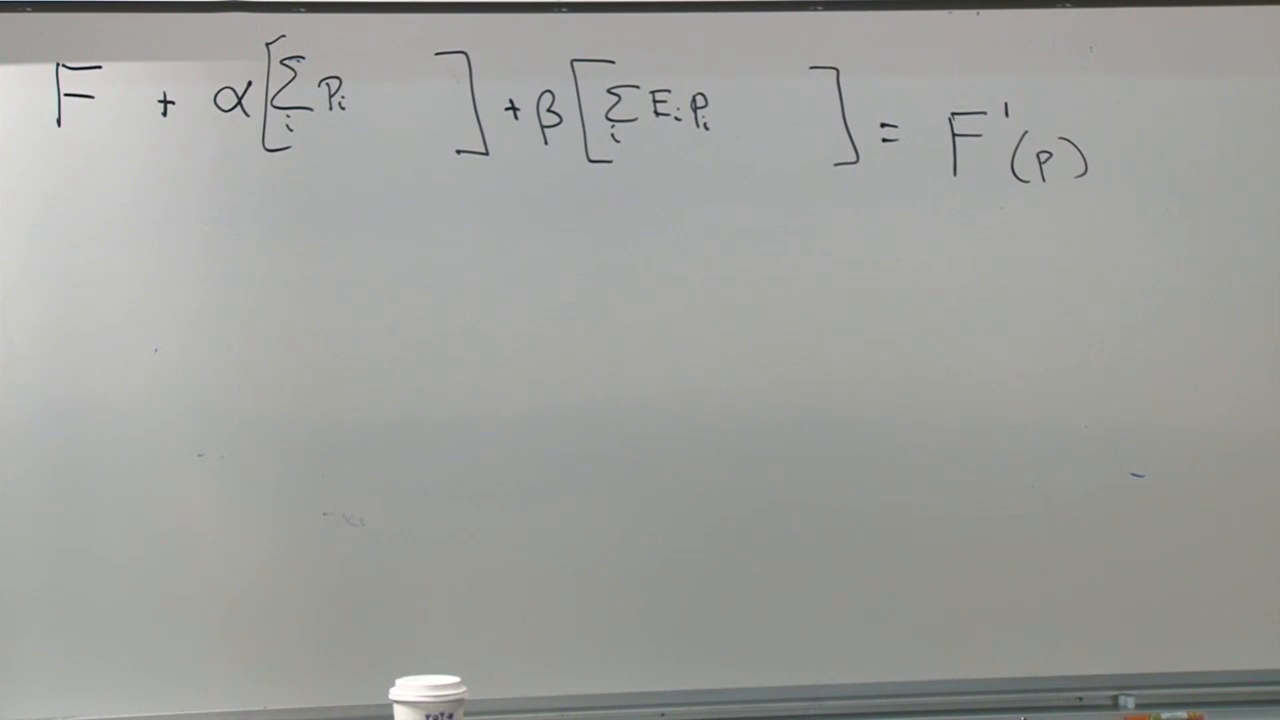
\includegraphics[width=0.92\textwidth]{lecture_04_figure_02.png}
\caption{確率の変分のもとで定数となる項を省略した後の拡張エントロピー汎関数。}
\lectureframe{00:10:56}
\end{figure}

確率に関して微分するとき、項\(-\alpha\)および\(-\beta E\)は何も寄与しない。これが黒板に見える省略された汎関数である。それらは\eqref{eq:sm4-augmented-functional}の一部であり続けるが、この特定の微分には無関係になっただけである。

\section{ボルツマン分布}

任意の一つの確率を選ぶ。講義では\(p_7\)を選ぶ。その理由の一部は、\(1\)が特別すぎるように見えることと、\(7\)が縁起の良い数であることである。この選択に依存するものは何もない。必要な微積分は
\begin{equation}
 \frac{d}{dp_i}\bigl(p_i\log p_i\bigr)=\log p_i+1.
\end{equation}
だけである。したがって
\begin{equation}
 \frac{\partial\Phi}{\partial p_i}
 =\log p_i+1+\alpha+\beta E_i=0.
 \label{eq:sm4-stationarity}
\end{equation}
\(p_i\)について解くと、
\begin{align}
 \log p_i&=-(1+\alpha)-\beta E_i,\\
 p_i&=e^{-(1+\alpha)}e^{-\beta E_i}.
\end{align}
第一の因子は状態ラベルに依存しない。これを\(1/Z\)と書く：
\begin{equation}
 p_i=\frac{e^{-\beta E_i}}{Z}.
 \label{eq:sm4-boltzmann-weight}
\end{equation}

これが最初の突然の報酬である。ありふれた制約付き微分から指数法則が生じた。相対確率は
\begin{equation}
 \frac{p_i}{p_j}=e^{-\beta(E_i-E_j)}.
 \label{eq:sm4-relative-weight}
\end{equation}
に従う。乗数\(\beta\)は、確率がエネルギーとともにどれほど急速に減少するかを制御する。大きな正の\(\beta\)は分布を最低準位の近くに集中させ、小さな正の\(\beta\)はかなりの重みをスペクトルのより上へ広げる。\(\beta\)を変えると平均エネルギーが変わることはすでに見て取れるが、それを逆温度と同定することはまだ証明されなければならない。

\section{正規化と分配関数}

正規化により状態に依存しない因子が決まる：
\begin{equation}
 1=\sum_i p_i
 =\frac{1}{Z}\sum_i e^{-\beta E_i},
\end{equation}
したがって
\begin{equation}
 Z(\beta)=\sum_i e^{-\beta E_i}.
 \label{eq:sm4-partition-function}
\end{equation}
これが正準分配関数である。最初は正規化定数として現れたが、その記述はその役割をひどく過小評価している。\(Z(\beta)\)がわかれば、熱力学的量はその微分から従う。

\eqref{eq:sm4-partition-function}におけるエネルギー準位は入力である。それらは系の力学と、固定された外部条件、すなわち箱の体積と形状、磁場または電場、その他の制御パラメータから来る。制御パラメータを変えるとスペクトルが変わり、したがって\(Z\)が変わる。当面の計算では、それらのパラメータ、ひいては集合\(\{E_i\}\)は固定されている。

\begin{classroomqa}
\audiencequestion{指数関数のスケッチの軸は正確には何を表すのか。縦座標は特定の\(p_i\)の一つなのか。}
\lecturerresponse{プロットされた高さは準位に割り当てられた確率であり、横方向の順序は状態ラベル\(i\)として、あるいはより物理的にはエネルギー\(E_i\)として読むことができる。各状態は固定されたエネルギーをもつ。\(\beta\)が大きいと、確率はそのエネルギーとともに急激に減少する。\(\beta=0\)の近くでは、重みはアクセス可能な準位にわたってほぼ平坦である。
\lecturetimestamp{00:19:39--00:20:09}}
\end{classroomqa}

\section{分配関数に隠れた平均エネルギー}

第二の拘束条件が\(\beta\)を決定する：
\begin{equation}
 E=\sum_i p_iE_i
 =\frac{1}{Z}\sum_i E_i e^{-\beta E_i}.
 \label{eq:sm4-mean-energy}
\end{equation}
この重み付き和を新たに評価するのではなく、
\eqref{eq:sm4-partition-function}を微分する：
\begin{equation}
 \frac{dZ}{d\beta}
 =-\sum_i E_i e^{-\beta E_i}.
\end{equation}
\eqref{eq:sm4-mean-energy}と比較すると
\begin{equation}
 E(\beta)
 =-\frac{1}{Z}\frac{dZ}{d\beta}
 =-\frac{d\log Z}{d\beta}.
 \label{eq:sm4-energy-logz}
\end{equation}
対数が自然対数であるのは、その導関数が因子
\(1/Z\)を与えるからである。

\begin{figure}[t]
\centering
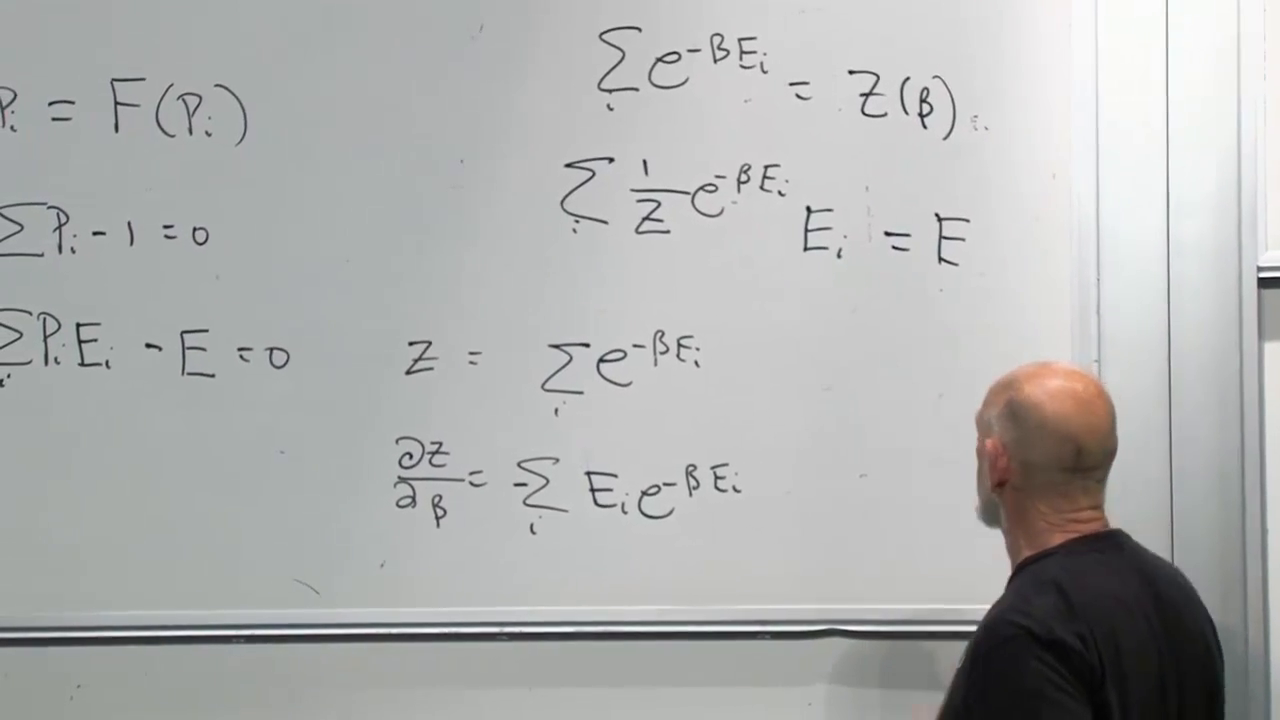
\includegraphics[width=0.82\textwidth]{lecture_04_figure_03.png}
\caption{正規化、平均エネルギーの拘束条件、および分配関数の導関数が黒板上に一緒に現れている。}
\lectureframe{00:26:24}
\end{figure}

\begin{classroomqa}
\audiencequestion{黒板の下の式は\(Z\)に対する新しい式なのか、それともその上の定義から得られるのか。}
\lecturerresponse{それは定義
\(Z=\sum_i e^{-\beta E_i}\)を微分することによって得られる。導関数は
\(-E_i\)を引き下ろす。その結果を\(Z\)で割ると、平均エネルギーを定義する重み付き和が再現される。
\lecturetimestamp{00:25:58--00:26:37}}
\end{classroomqa}

\begin{classroomqa}
\audiencequestion{
\(dZ/d\beta=-E Z\)は\(Z\)を微分の固有関数にするか。}
\lecturerresponse{通常の意味ではそうではない。固有値方程式では\(Z\)に定数が掛かるのに対し、ここでは
\(E=E(\beta)\)である。この式は\(\beta\)の関数としての平均エネルギーを述べているのであり、固定固有値問題ではない。
\lecturetimestamp{00:28:49--00:29:43}}
\end{classroomqa}

\eqref{eq:sm4-energy-logz}の単純さは見かけにすぎない。スペクトルは複雑かもしれず、\(Z\)の計算は困難でありうるが、その一つの関数さえ見つかれば、平均エネルギーは一回の微分で得られる。このパターンは統計力学の至るところで繰り返される：正しい順序で適用された初等的な操作が、直接推測するのは難しかったであろう結果をもたらすのである。

\begin{classroomqa}
\audiencequestion{\(E\)はすべての複製の全エネルギーなのか、それとも一箱あたりの平均エネルギーなのか。}
\lecturerresponse{それは一箱の平均エネルギーである。複製の集まりは全エネルギー\(\mathcal N E\)をもつ。後に、系そのものが\(N\)個の気体粒子を含む一箱全体として選ばれるとき、\(E\)はその気体試料全体のエネルギーを意味することになる。
\lecturetimestamp{00:30:55--00:31:10}}
\end{classroomqa}

\begin{classroomqa}
\audiencequestion{
\(\sum_i e^{-\beta E_i}\)の対数を項ごとに取ることはできるか。}
\lecturerresponse{いいえ。対数は積を和に変えるのであって、和を対数の和に変えるのではない：
\[
 \log\!\left(\sum_i e^{-\beta E_i}\right)
 \ne \sum_i\log\!\left(e^{-\beta E_i}\right).
\]
この区別は、独立な部分系がそれらの分配関数を掛け合わせるようになる後で役に立つ。
\lecturetimestamp{00:31:10--00:31:58}}
\end{classroomqa}

\section{何が固定され、何が変化を許されるのか}

同じ式の中にいくつかの層の変数があり、教室での議論はそれらを意図的に区別している。

\begin{itemize}
 \item 確率\(p_i\)は元々の未知数である。
 \item 準位\(E_i\)は、系とその制御パラメータが指定されれば固定される。
 \item 乗数\(\alpha\)は正規化\(Z=e^{1+\alpha}\)に吸収されている。
 \item 規定された平均エネルギー\(E\)に対して、拘束条件は一つの数\(\beta\)を固定する。しかし平衡状態の族にわたっては、\(E=E(\beta)\)または\(\beta=\beta(E)\)のいずれかを用いることができる。
\end{itemize}

\begin{classroomqa}
\audiencequestion{乗数が数であるなら、なぜ\(\beta\)と\(E\)が今変数として扱われるのか。}
\lecturerresponse{一つの拘束問題に対しては、それらは確かに数である。しかし、同じスペクトルと同じでない規定された平均エネルギーをもつ多くの平衡問題を比較することができる。その族に沿って、\(\beta\)は\(E\)とともに変化する。\(E\)を固定すれば\(\beta\)が決まり、\(\beta\)を固定すれば\(E\)が決まる。これらは同じ関係の二つの読み方である。
\lecturetimestamp{00:31:58--00:33:27}}
\end{classroomqa}

\begin{classroomqa}
\audiencequestion{\(\alpha\)は消えてしまったのか。}
\lecturerresponse{消えたのはその名前だけである。定義
\(e^{-(1+\alpha)}=1/Z\)がそれを\(Z\)に吸収する。\(\alpha\)と\(Z\)の両方を保つと、同じ正規化パラメータを二重に数えることになる。
\lecturetimestamp{00:33:29--00:33:49}}
\end{classroomqa}

エネルギーだけが唯一の保存量である必要はない。全運動量、粒子数、角運動量、または別の量が拘束されているなら、その期待値はそれ自身の乗数を受け取る。その拡張はアンサンブルを変えるが、方法は変えない。

\begin{classroomqa}
\audiencequestion{平均エネルギーだけを固定することは、系についてあまりに多くを仮定しすぎるのではないか。}
\lecturerresponse{それは、現在の問題において条件付けを必要とする他の保存量が存在しないことを仮定している。たとえば全運動量も固定されているなら、別の拘束条件と別のラグランジュ乗数を加えればよい。対照的に、体積、形状、および外部場はここでは制御パラメータである：それらは固定されており、エネルギー準位そのものを決定する。
\lecturetimestamp{00:33:51--00:35:50}}
\end{classroomqa}

\begin{classroomqa}
\audiencequestion{\(\alpha\) はエネルギーのもう一つの引数として現れるべきなのか、また \(Z\) は準位 \(E_i\) に依存するのか。}
\lecturerresponse{\(\alpha\) はすでに \(Z\) に含まれているので、独立な引数ではない。分配関数は確かに固定されたスペクトルにも \(\beta\) にも依存する。制御パラメータを変えると \(E_i\) が変わり、したがって \(Z\) も変わる。現在の \(\beta\) に関する微分の間は、スペクトルは固定して保たれる。
\lecturetimestamp{00:35:52--00:37:10}}
\end{classroomqa}

\begin{classroomqa}
\audiencequestion{我々は個々の準位\(E_i\)を変化させているのか、それとも平均エネルギー\(E\)を変化させているのか。}
\lecturerresponse{個々の準位は固定されたままである。平均エネルギーは確率が変化するために変化する。したがって、この族は\(E\)によって、あるいは同等に\(\beta\)によってパラメータ付けられ、同じ準位のリスト\(\{E_i\}\)が全体を通して用いられる。
\lecturetimestamp{00:37:12--00:39:04}}
\end{classroomqa}

実際には、温度は気体の全エネルギーよりもはるかに測定しやすいことが多い。温度計を挿入することができる。相対論的質量差を秤量して\(E=mc^2\)を援用するのは正しいが、著しく役に立たない。\(\beta\)を操作可能にするには、今度はそれを温度の熱力学的定義に結び付けなければならない。

\section{温度より先にエントロピー}

エントロピーが論理的には先に来る。ボルツマン確率を\eqref{eq:sm4-entropy}に代入すると、
\begin{equation}
 \log p_i=-\beta E_i-\log Z.
\end{equation}
すると
\begin{align}
 S
 &=-\sum_i p_i\log p_i\\
 &=\beta\sum_i p_iE_i+\log Z\sum_i p_i\\
 &=\beta E+\log Z.
 \label{eq:sm4-entropy-logz}
\end{align}
規格化の和が最後の因子1を与える。これはまたヘルムホルツ自由エネルギーの最初の兆候でもある。なぜなら後に\(F_{\mathrm H}=-T\log Z\)となるからである。ただし\(k_B=1\)の単位である。

\begin{classroomqa}
\audiencequestion{第一項の因子\(1/Z\)はどうなったのか。}
\lecturerresponse{それはすでに\(p_i\)の一部である。和\(\sum_i p_iE_i\)は完全な規格化された確率を含み、定義により平均エネルギー\(E\)である。
\lecturetimestamp{00:43:19--00:43:26}}
\end{classroomqa}

\begin{classroomqa}
\audiencequestion{\(S=\beta E+\log Z\)に負号があるべきではないか。}
\lecturerresponse{いいえ。エントロピーは負号で始まるが、\(\log p_i=-\beta E_i-\log Z\)はさらに二つの負号を含む。それらは\eqref{eq:sm4-entropy-logz}に示された二つの正の項を生じる。
\lecturetimestamp{00:45:53--00:46:03}}
\end{classroomqa}

温度は熱力学的に
\begin{equation}
 dE=T\,dS,
 \qquad
 \frac{1}{T}=\frac{dS}{dE},
 \label{eq:sm4-temperature-definition}
\end{equation}
によって定義された。ただし他のすべての制御パラメータは固定されている。\eqref{eq:sm4-entropy-logz}を直接\(E\)で微分する最初の試みは、\(\beta\)も\(E\)に依存するため、すぐに煩雑になる。全微分を取る方がすっきりしている。
\begin{align}
 dS
 &=\beta\,dE+E\,d\beta
   +\frac{d\log Z}{d\beta}\,d\beta\\
 &=\beta\,dE+E\,d\beta-E\,d\beta\\
 &=\beta\,dE.
 \label{eq:sm4-entropy-differential}
\end{align}
この相殺は\eqref{eq:sm4-energy-logz}を用いている。\eqref{eq:sm4-entropy-differential}と\eqref{eq:sm4-temperature-definition}を比較すると
\begin{equation}
 T=\frac{1}{\beta},
 \qquad
 \beta=\frac{1}{T}.
 \label{eq:sm4-beta-temperature}
\end{equation}

\begin{figure}[t]
\centering
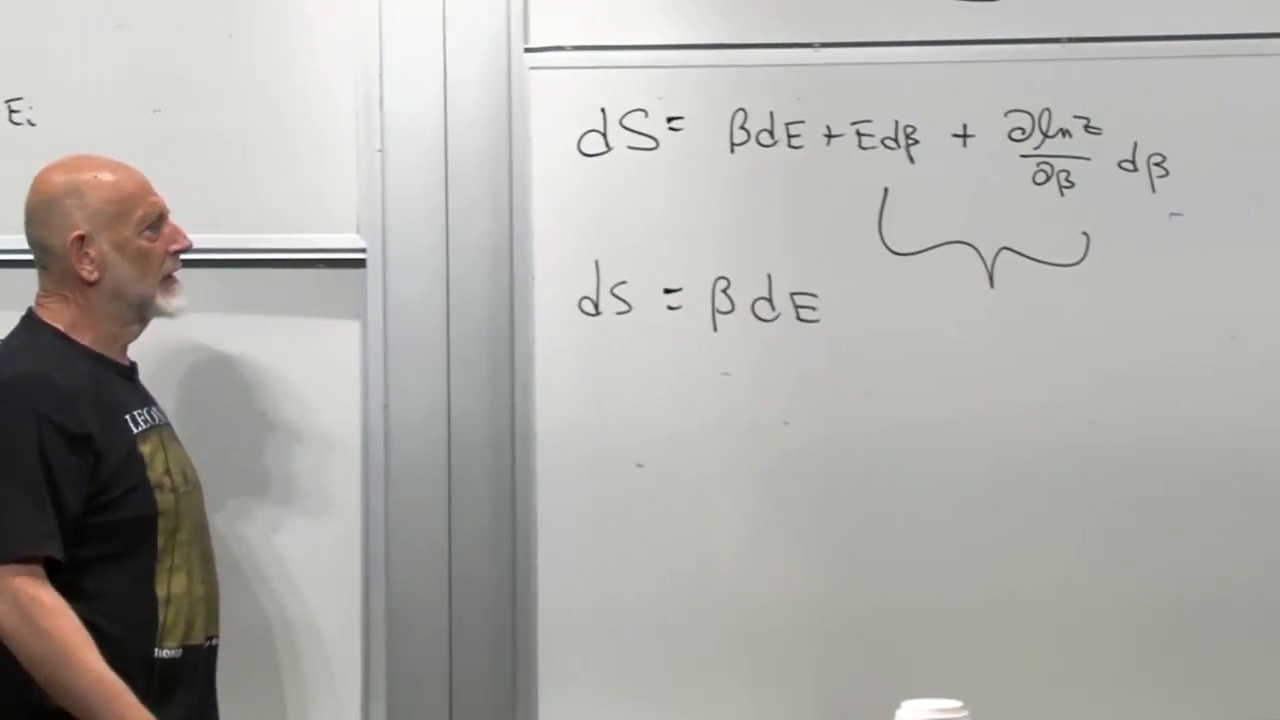
\includegraphics[width=0.82\textwidth]{lecture_04_figure_04.png}
\caption{二つの\(d\beta\)項が相殺し、\(dS=\beta\,dE\)が残る。}
\lectureframe{00:50:48}
\end{figure}

\begin{classroomqa}
\audiencequestion{この相殺は\(\log Z\)がエネルギーや温度から独立であると誤って仮定しているのではないか。}
\lecturerresponse{いいえ。固定されたスペクトルに対しては、独立な熱的パラメータが一つある。\(Z=Z(\beta)\)と書くことができ、次に平衡族に沿って\(\beta=\beta(E)\)とみなすことができる。全微分は完全な\(d\beta\)依存性を保ち、恒等式\(d\log Z/d\beta=-E\)がまさに相殺を成立させている。
\lecturetimestamp{00:52:04--00:52:44}}
\end{classroomqa}

計算のほとんどの間、温度はエネルギー単位で測られるので、\(k_B=1\)である。実験室単位に戻すと、
\begin{equation}
 \beta=\frac{1}{k_B T_{\mathrm K}},
 \label{eq:sm4-beta-laboratory}
\end{equation}
ここで\(T_{\mathrm K}\)はケルビンで表した絶対温度である。\(T_{\mathrm e}=k_BT_{\mathrm K}\)と書いてから\(\beta=1/T_{\mathrm e}\)を用いるのがしばしば便利である。

\begin{classroomqa}
\audiencequestion{気体のある体積について、系は一分子なのか、それとも全体の集まりなのか。}
\lecturerresponse{それは系をどのように定義するかによる。ここでは系は気体の箱全体であり、したがって\(E\)はそのすべての分子のエネルギーである。十分に希薄な理想気体では、粒子が相互作用しないため、一分子も部分系として扱うことができる。以下の因子分解が二つの記述の関係を示すであろう。
\lecturetimestamp{00:53:32--00:54:49}}
\end{classroomqa}

正準集団の恒等式をここでまとめておく。
\begin{align}
 p_i&=\frac{e^{-\beta E_i}}{Z},&
 Z(\beta)&=\sum_i e^{-\beta E_i},\label{eq:sm4-canonical-pair}\\
 E&=-\frac{d\log Z}{d\beta},&
 S&=\beta E+\log Z,&
 T&=\frac{1}{\beta}.
 \label{eq:sm4-canonical-identities}
\end{align}

\section{古典的理想気体}

体積\(V\)の箱の中に質量\(m\)の同一な点粒子\(N\)個を取る。粒子間の相互作用が無視できるとき、気体は理想的である。これは、力が弱いため、あるいは気体が十分に希薄で近接遭遇が稀であるため、良い近似となりうる。

古典的微視的状態はすべての位置と運動量によって指定される。
\begin{equation}
 (\bm q_1,\ldots,\bm q_N;\bm p_1,\ldots,\bm p_N).
\end{equation}
位置座標が\(3N\)個、運動量座標が\(3N\)個あるので、状態は\(6N\)次元の位相空間の一点である。相互作用がなければ、ハミルトニアンは
\begin{equation}
 H(\bm p)=\sum_{a=1}^{N}\frac{\bm p_a^2}{2m}
 =\sum_{\mu=1}^{3N}\frac{p_\mu^2}{2m}.
 \label{eq:sm4-ideal-hamiltonian}
\end{equation}

\begin{classroomqa}
\audiencequestion{粒子は\(3N\)個あり、すべての運動量成分について和をとると状態を二重に数えることになるのか。}
\lecturerresponse{粒子は\(N\)個、運動量成分は\(3N\)個である。\eqref{eq:sm4-ideal-hamiltonian}の和には、各成分に対して二次の項が1つずつ含まれる。すると相空間積分は各独立成分をちょうど1回ずつ積分するので、その積から二重計数は生じない。
\lecturetimestamp{01:02:29--01:04:04}}
\end{classroomqa}

連続的な古典相空間では、状態和は
\begin{equation}
 Z_N
 =\frac{1}{N!\,h^{3N}}
 \int_{V^N}d^{3N}q
 \int_{\mathbb R^{3N}}d^{3N}p\,
 e^{-\beta H(\bm p)}.
 \label{eq:sm4-classical-partition}
\end{equation}
となる。講義では積分に焦点を当て、相空間のセル\(h^{3N}\)を書かずに同じ表式を記す。これを復元すると\(Z_N\)が無次元になり、古典的な状態数え上げの量子的起源が記録される。\(h\)は\(\beta\)に依存しないので、以下で用いるエネルギー微分を変えない。

位置積分は直ちに実行できる。ハミルトニアンは位置に依存せず、各粒子は箱の中のどこにでも存在しうる：
\begin{equation}
 \int_{V^N}d^{3N}q=V^N.
\end{equation}
運動量積分は\(3N\)個の同一な一次元ガウス積分に因子分解される：
\begin{equation}
 Z_N
 =\frac{V^N}{N!\,h^{3N}}
 \left[
  \int_{-\infty}^{\infty}dp\,
  e^{-\beta p^2/(2m)}
 \right]^{3N}.
 \label{eq:sm4-factorized-gas}
\end{equation}

因子\(1/N!\)は、同一粒子の置換によってのみ異なる配置を同定する。固定された\(N\)と\(V\)における平均エネルギーに対しては、\(\log Z_N\)に\(\beta\)に依存しない定数を加えるだけなので、\(-\partial/\partial\beta\)の下で消える。しかしすべての問いにおいて不要というわけではない：\(h^{3N}\)とともに、無次元の分配関数、示量的なエントロピー、そして整合的な化学ポテンシャルにとって不可欠である。

ここで
\begin{equation}
 x=\sqrt{\frac{\beta}{2m}}\,p,
 \qquad
 dp=\sqrt{\frac{2m}{\beta}}\,dx.
\end{equation}
と置く。ガウス積分は
\begin{align}
 \int_{-\infty}^{\infty}dp\,e^{-\beta p^2/(2m)}
 &=
 \sqrt{\frac{2m}{\beta}}
 \int_{-\infty}^{\infty}dx\,e^{-x^2}\\
 &=\sqrt{\frac{2\pi m}{\beta}}.
 \label{eq:sm4-gaussian}
\end{align}
となる。

\begin{figure}[t]
\centering
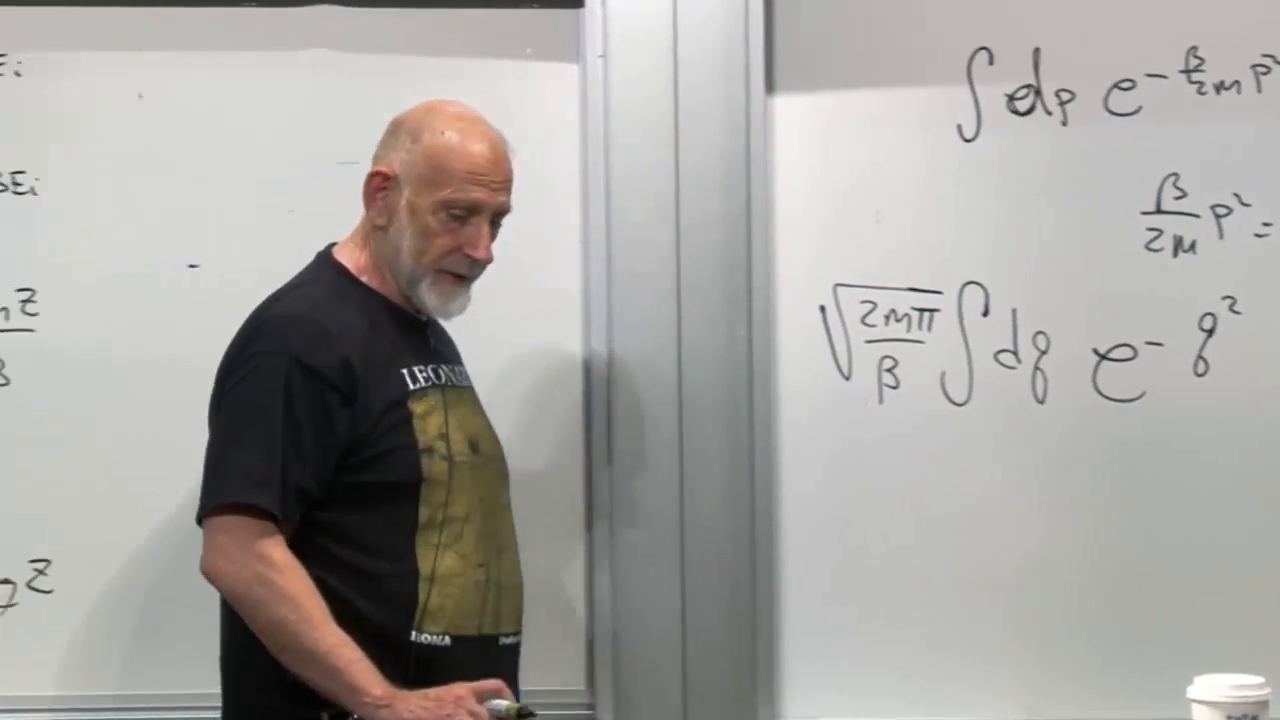
\includegraphics[width=0.82\textwidth]{lecture_04_figure_05.png}
\caption{運動量積分は、1回のスケーリングによって標準的なガウス積分に帰着される。}
\lectureframe{01:13:12}
\end{figure}

\eqref{eq:sm4-factorized-gas}に代入すると
\begin{equation}
 Z_N
 =\frac{V^N}{N!\,h^{3N}}
 \left(\frac{2\pi m}{\beta}\right)^{3N/2}.
 \label{eq:sm4-ideal-partition}
\end{equation}
を得る。

\begin{figure}[t]
\centering
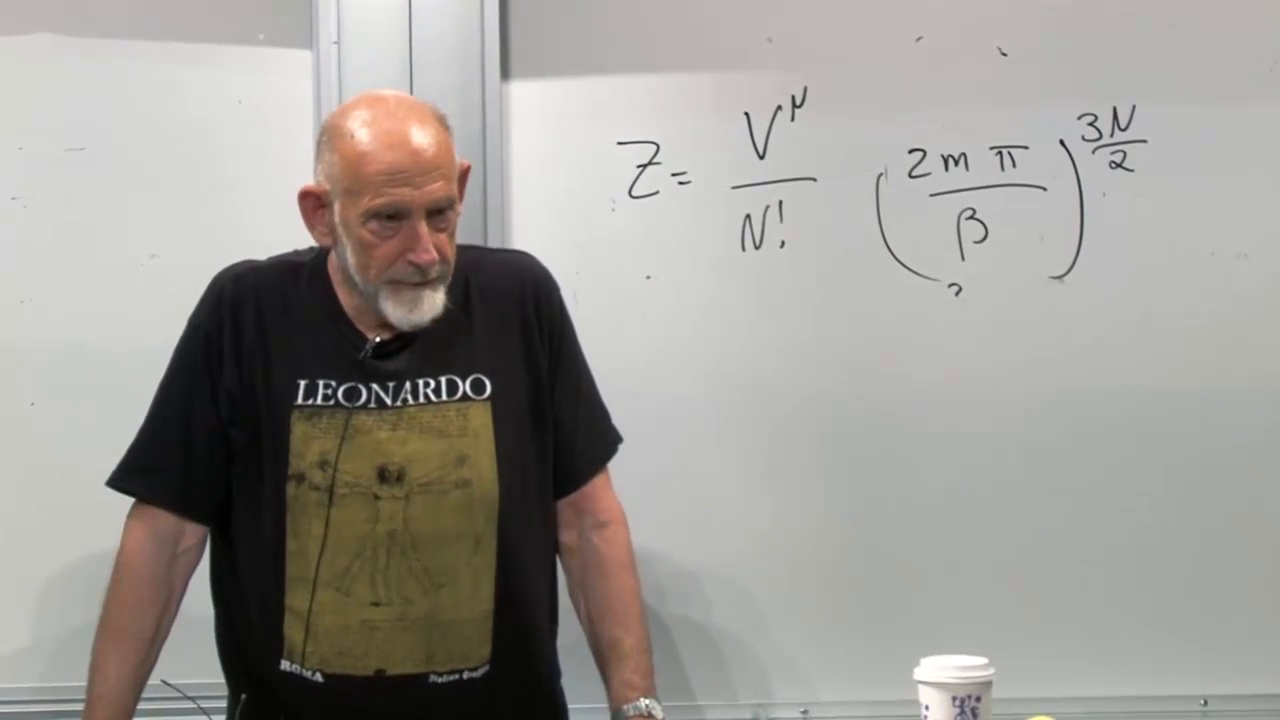
\includegraphics[width=0.78\textwidth]{lecture_04_figure_06.png}
\caption{黒板に完成した理想気体の分配関数。相空間のセル\(h^{3N}\)は\eqref{eq:sm4-ideal-partition}において復元されている。}
\lectureframe{01:14:38}
\end{figure}

同じ結果を熱的ド・ブロイ波長
\begin{equation}
 \lambda_T=\frac{h}{\sqrt{2\pi mT}}
 \qquad (k_B=1).
\end{equation}
でまとめておくと便利である。すると
\begin{equation}
 Z_N=\frac{1}{N!}\left(\frac{V}{\lambda_T^3}\right)^N.
 \label{eq:sm4-thermal-wavelength-form}
\end{equation}
となる。

巨視的な\(N\)に対して、スターリングの公式は
\begin{equation}
 N!\simeq N^Ne^{-N}\sqrt{2\pi N}.
\end{equation}
を与える。主要な指数依存性のみを残し、
\(\rho=N/V\)
と定義すると、
\begin{equation}
 \frac{V^N}{N!}
 \simeq
 \frac{1}{\sqrt{2\pi N}}
 \left(\frac{e}{\rho}\right)^N.
 \label{eq:sm4-density-rewrite}
\end{equation}
となる。これが講義の簡潔な密度による書き換えである。平方根の因子は\(\log Z_N\)において次次の寄与であるが、ここでは黙って落とすのではなく明示している。

\begin{classroomqa}
\audiencequestion{\(1/N!\)が\(\beta\)に依存しないなら、まったく違いを生じないのか。}
\lecturerresponse{固定された\(N\)と\(V\)における現在の平均エネルギー微分には違いを生じない。なぜなら\(\log Z_N\)に\(\beta\)に依存しない定数を加えるからである。しかし絶対エントロピーや粒子数の変動に対しては重要である。限定的な微分についての言明と、より広い状態数え上げについての言明を混同してはならない。
\lecturetimestamp{01:27:01--01:27:51}}
\end{classroomqa}

\section{エネルギーと等分配}

積は微分しにくいが、対数をとれば和になる。\eqref{eq:sm4-ideal-partition}より、
\begin{equation}
 \log Z_N
 =-\frac{3N}{2}\log\beta+\text{\(\beta\)-independent terms}.
 \label{eq:sm4-log-ideal-partition}
\end{equation}
したがって
\begin{equation}
 E
 =-\frac{\partial\log Z_N}{\partial\beta}
 =\frac{3N}{2\beta}
 =\frac{3N}{2}T.
 \label{eq:sm4-ideal-energy}
\end{equation}
粒子あたりのエネルギーは
\begin{equation}
 \frac{E}{N}=\frac{3}{2}T
 \qquad (k_B=1),
\end{equation}
あるいは実験室単位では
\begin{equation}
 \frac{E}{N}=\frac{3}{2}k_BT_{\mathrm K}.
 \label{eq:sm4-ideal-energy-lab}
\end{equation}
である。

\begin{figure}[t]
\centering
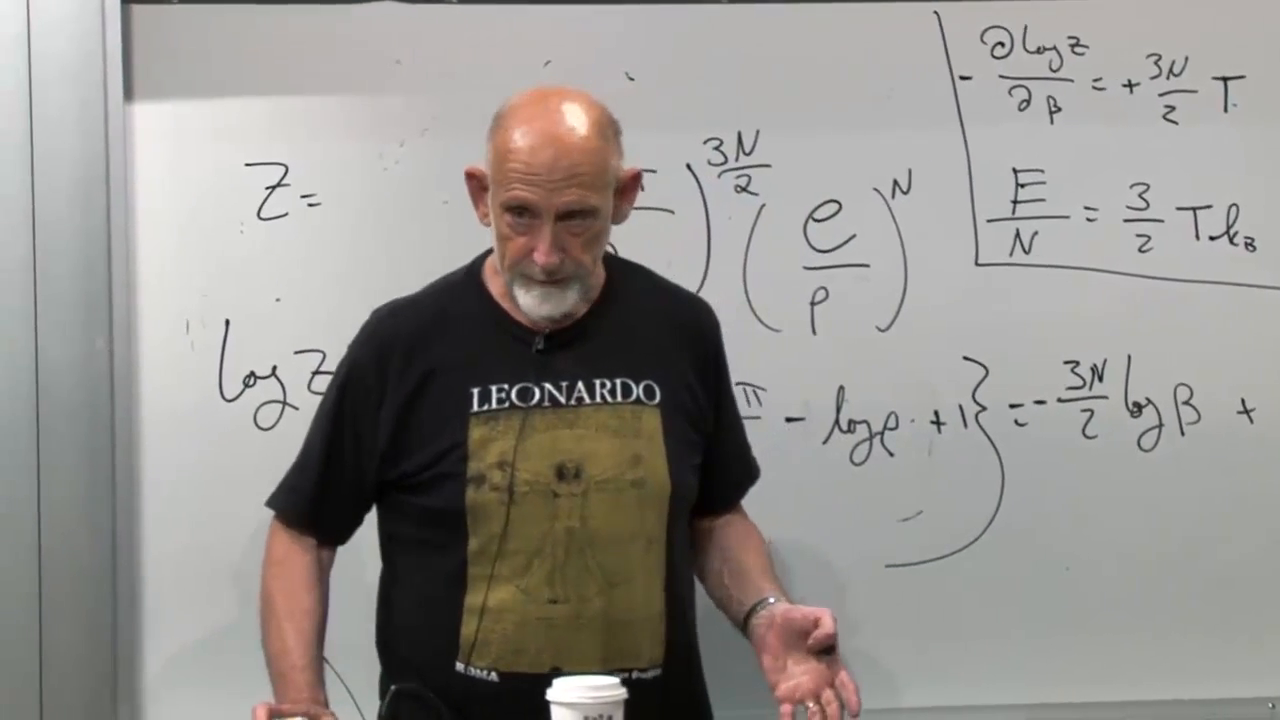
\includegraphics[width=0.84\textwidth]{lecture_04_figure_07.png}
\caption{理想気体のエネルギーに寄与するのは\(-3N\log\beta/2\)の項のみであり、\(E/N=3T/2\)を与える。}
\lectureframe{01:25:28}
\end{figure}

\begin{classroomqa}
\audiencequestion{エネルギーの式にはボルツマン定数はどこから入るのか。}
\lecturerresponse{理論家の温度\(T\)はエネルギーである。ケルビンを用いるには、これを\(k_BT_{\mathrm K}\)に置き換えれば
\(E/N=3k_BT_{\mathrm K}/2\)
となる。\(k_B\)の小さな値が、巨視的に見える数値温度を1分子の微視的エネルギー尺度に変換する。
\lecturetimestamp{01:24:58--01:26:01}}
\end{classroomqa}

3は空間の3方向から来る。1/2は各ガウス積分の\(1/\beta\)への平方根依存性から来る。各独立な二次の運動量座標は平均エネルギーに
\begin{equation}
 \frac{1}{2}T
\end{equation}
を寄与する。\(d\)次元空間では同じ議論により
\(E/N=dT/2\)
となる。これが等分配の最初の出現である。

講義の最後に課題として与えられたエントロピー計算は\(S=\beta E+\log Z_N\)から従う。スターリング近似を用いると、
\begin{equation}
 \frac{S}{N}
 \simeq
 \log\!\left[
  \frac{V}{N}
  \left(\frac{2\pi mT}{h^2}\right)^{3/2}
 \right]
 +\frac{5}{2},
 \label{eq:sm4-sackur-tetrode}
\end{equation}
が、有限\(N\)の次次の補正まで成り立つ。\(k_B\)を復元すると右辺に\(k_B\)が掛かり、\(T\)が\(k_BT_{\mathrm K}\)に置き換わる。この結果は、エネルギーから落ちていた規格化因子がエントロピーにとって不可欠である理由を明らかにする。

\section{気体を重力場に置く}

箱を中性子星の上に置くという問いは、重力への拡張を導入する。中性子星に立ち向かう前に、普通の部屋の中の一様な場\(g\)を考えよう。底面積\(A\)、高さ\(L\)の箱の底面で\(y=0\)を選ぶ。ハミルトニアンは
\begin{equation}
 H=\sum_{a=1}^{N}
 \left(\frac{\bm p_a^2}{2m}+mgy_a\right).
 \label{eq:sm4-gravity-hamiltonian}
\end{equation}
となる。水平方向の位置積分は依然として\(A^N\)を与え、各鉛直座標は
\begin{equation}
 I_y(L)
 =\int_0^Ldy\,e^{-\beta mgy}
 =\frac{1-e^{-\beta mgL}}{\beta mg}.
 \label{eq:sm4-finite-height-integral}
\end{equation}
に寄与する。

\begin{classroomqa}
\audiencequestion{鉛直方向の積分は本当に無限大まで及ぶべきなのか、それとも箱の上端までなのか。}
\lecturerresponse{有限の箱に対しては、\eqref{eq:sm4-finite-height-integral}のように、\(0\)からその高さ\(L\)まで及ばなければならない。上限を無限大にとるのは、有限の部屋ではなく表面上の大気をモデル化する、後段での単純化である。
\lecturetimestamp{01:30:25--01:31:32}}
\end{classroomqa}

したがって、有限の高さに対する完全な分配関数は
\begin{equation}
 Z_N(L)
 =
 \frac{1}{N!\,h^{3N}}
 \left[
  A\,
  \frac{1-e^{-\beta mgL}}{\beta mg}
  \left(\frac{2\pi m}{\beta}\right)^{3/2}
 \right]^N.
 \label{eq:sm4-gravity-partition-finite}
\end{equation}
である。鉛直方向の因子は\(\beta\)に依存するので、エネルギーに寄与しなければならない。実際、
\begin{equation}
 \langle U\rangle
 =N\left[
  \frac{1}{\beta}
  -\frac{mgL}{e^{\beta mgL}-1}
 \right].
 \label{eq:sm4-finite-gravity-energy}
\end{equation}
である。これで、講義で最初は厄介な計算として残された積分の小さな部分が完成する。

無限に高い大気、すなわち\(L\to\infty\)の場合、
\begin{equation}
 I_y(\infty)=\frac{1}{\beta mg}.
\end{equation}
である。分配関数は
\begin{equation}
 Z_N^{(\infty)}
 =
 \frac{1}{N!\,h^{3N}}
 \left[
  \frac{A}{\beta mg}
  \left(\frac{2\pi m}{\beta}\right)^{3/2}
 \right]^N.
 \label{eq:sm4-gravity-partition-infinite}
\end{equation}
となる。その\(\beta\)に依存する対数は
\begin{equation}
 \log Z_N^{(\infty)}
 =-\frac{3N}{2}\log\beta-N\log\beta+\mathrm{const}.
\end{equation}
である。第一項は運動エネルギー\(3NT/2\)を与え、第二項は平均重力ポテンシャルエネルギー\(NT\)を与える。したがって、この理想化された非有界大気に対して
\begin{equation}
 E_{\mathrm{tot}}=\frac{5N}{2}T
\end{equation}
である。

\begin{figure}[t]
\centering
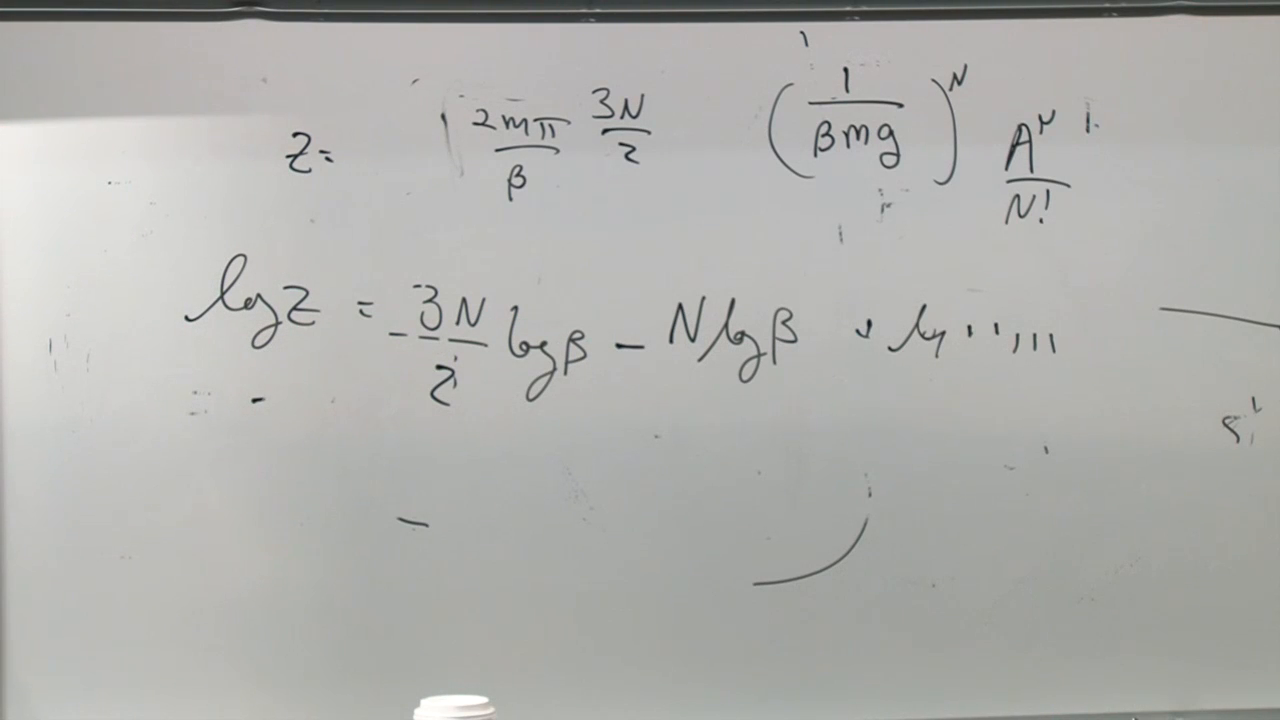
\includegraphics[width=0.83\textwidth]{lecture_04_figure_08.png}
\caption{無限大気の分配関数は、平均ポテンシャルエネルギーの源である\(-N\log\beta\)を\(\log Z\)に加える。}
\lectureframe{01:36:38}
\end{figure}

\begin{classroomqa}
\audiencequestion{非常に強い重力場には別のラグランジュ乗数が必要になるのだろうか。}
\lecturerresponse{単に場が強いからという理由ではない。重力はハミルトニアンを変え、したがってエネルギー準位または位相空間の重みを変える。同じエネルギー乗数\(\beta\)が残る。中性子星はさらなる物理的複雑さをもたらすが、最初の修正は依然として重力ポテンシャルエネルギーを\(H\)に入れることである。
\lecturetimestamp{01:27:58--01:29:24}}
\end{classroomqa}

\section{最後に三つの問い}

\begin{classroomqa}
\audiencequestion{どの方程式がボルツマン分布であり、それは平衡について何を主張するのか。}
\lecturerresponse{その分布は
\[
 p_i=\frac{e^{-\beta E_i}}{Z}.
\]
である。これは規格化と固定された平均エネルギーという条件の下での最大エントロピー分布である。平均エネルギーは同じ確率から計算しなければならず、規格化は最終式ではほとんど自動的に見えても、依然として課さなければならない。
\lecturetimestamp{01:38:14--01:38:45}}
\end{classroomqa}

手順は機械的に感じられるかもしれない。分配関数を書き、対数をとり、微分する。それでも、得られる方程式は驚きに満ち続けている。慣れによって、どの単純な操作がどの操作に続くべきかは分かるが、それによってこの主題の不思議さが減るわけではない。

\begin{classroomqa}
\audiencequestion{これらのエントロピーの考えは、崩壊する恒星やブラックホールに適用できるのか。物質がより小さな領域を占めるのに、どうしてエントロピーが増大しうるのか。}
\lecturerresponse{恒星が難しいのは主に、その物質の詳細が複雑だからである。ブラックホールにはより明快な基準がある。そのベッケンシュタイン--ホーキングエントロピーは、与えられた巨視的制約に対する極限的な重力エントロピーである。崩壊はそのブラックホールの値に達するまでエントロピーを増大させうる。それ以上増大させるには、利用可能なエネルギーまたは大きさを変える必要がある。
\lecturetimestamp{01:39:29--01:40:36}}
\end{classroomqa}

\begin{classroomqa}
\audiencequestion{分配関数はエネルギーの揺らぎも計算できるのか。}
\lecturerresponse{はい。一階微分は平均エネルギーを与え、二階微分はその分散を与える。
\begin{align*}
 \frac{\partial^2\log Z}{\partial\beta^2}
 &=\langle E^2\rangle-\langle E\rangle^2\\
 &=\operatorname{Var}(E).
\end{align*}
エネルギー単位では、これは熱容量と\(\operatorname{Var}(E)=T^2C_V\)の関係にある。実験室単位では、
\(\operatorname{Var}(E)=k_BT_{\mathrm K}^2C_V\)
である。この揺らぎの関係が次の計算である。
\lecturetimestamp{01:40:37--01:41:53}}
\end{classroomqa}

揺らぎは、統計力学を純粋に連続的な熱力学記述から区別する。特にギブズとアインシュタインに結びつけられるその系統的研究は、滑らかな巨視的法則の背後にある有限の微視的構成要素を明らかにする。次回の講義はそこから始まる。
\chapter{圧力、自由エネルギー、およびエネルギーの揺らぎ}

\lectureoverview{分子が壁に衝突するという運動論的描像を仮定することなく、分配関数から圧力を導出する。幾何学的補題によって断熱微分を固定温度での微分に変換し、ヘルムホルツ自由エネルギーが\(\log Z\)への橋渡しを与え、その最初の応用として理想気体の法則が導かれる。次に同じ分配関数を用いて平衡状態におけるエネルギーの揺らぎと、それが熱容量と持つ関係を導出する。}

\section{数学に直観を試させる}

熱力学は独特な評判を持っている。その計算は初等的であるが、何を微分し何を固定するかの選択は驚くほど微妙でありうる。我々の問題は意図的に狭い。すなわち理想気体の圧力を計算することである。しかしその答えへの道筋は、慣れ親しんだ分子的描像がもはや信頼できないような系にも十分一般に適用できるように意図されている。

運動論的な説明は容易である。分子は壁に衝突し、その運動量の法線成分を反転させる。単位時間あたりに受け渡される運動量が力を与え、単位面積あたりの力が圧力を与える。三次元における分子一個あたりの平均運動エネルギーが
\begin{equation}
 \left\langle \frac{p^2}{2m}\right\rangle=\frac{3}{2}T
 \qquad (k_B=1).
 \label{eq:sm5-mean-kinetic-energy}
\end{equation}
であることはすでに知っている。等方的な速度分布があれば、衝突率、各衝突における運動量の移動、そして結果として生じる圧力を見積もることができる。

しかし壁そのものが等方性を損なうように思われる。なぜ境界のごく近くにある分子が、内部深くにある分子と同じ速さと方向の分布を持つべきであろうか。平衡状態では、ここで関係する精度においてはそうであるが、その結論は直観として計算に紛れ込ませるのではなく、統計力学から導かれるべきものである。分子間の衝突は運動論的議論をさらに不透明にする。無相互作用気体が容易であるのは、まさにそれが異常に単純な系だからである。

物理学には、描像を一時的に抑えて数学に身を委ねることが最も安全な手続きとなる場合がある。求めるべき量を特定し、一般関係を操作し、認識できる公式が現れるまで待つのである。直観は最後に戻ってくるが、そのときには数学が直観を試しているのであって、その逆ではない。熱力学の喜びは、この手続きから現れる驚くべき関係にある。

求める関係は状態方程式であり、
\begin{equation}
 P=P(T,V,N),
 \label{eq:sm5-equation-of-state-target}
\end{equation}
ここで\(N\)は物質量、\(T\)は温度、\(V\)は体積である。満足のいく導出は、粒子が相互作用する場合や、物質が液体、プラズマ、固体である場合にも引き続き意味をなすべきである。分配関数の最終的な評価においてのみ、理想気体に特殊化される。

\section{エントロピーとヘルムホルツ自由エネルギー}

後に必要となる正準公式をまず思い出そう。\(i\)でラベル付けされたミクロ状態に対して、
\begin{equation}
 \begin{aligned}
 S&=-\sum_i p_i\log p_i,\\
 p_i&=\frac{e^{-\beta E_i}}{Z},\\
 Z&=\sum_i e^{-\beta E_i}.
 \end{aligned}
 \label{eq:sm5-canonical-definitions}
\end{equation}
確率の対数は
\begin{equation}
 \log p_i=-\beta E_i-\log Z.
 \label{eq:sm5-log-probability}
\end{equation}
これをエントロピーに代入すると
\begin{align}
 S
 &=-\sum_i p_i\log p_i \notag\\
 &=\beta\sum_i p_iE_i+\log Z\sum_i p_i \notag\\
 &=\beta E+\log Z.
 \label{eq:sm5-entropy-log-z}
\end{align}
ここで\(E=\sum_i p_iE_i\)は平均エネルギーである。

\begin{classroomqa}
\audiencequestion{なぜ第二項は、状態数かける\(\log Z\)ではなく、\(\log Z\)だけを与えるのですか。}
\lecturerresponse{和をとっている係数は\(1\)ではなく\(p_i\)である。規格化により\(\sum_i p_i=1\)が成り立つ。等価に言えば、分子\(\sum_i e^{-\beta E_i}=Z\)が分母の\(Z\)を打ち消す。この段階で状態数は決して現れない。
\lecturetimestamp{00:14:25--00:14:55}}
\end{classroomqa}

講義の大部分で用いているエネルギー単位では、
\(\beta=1/T\)である。\eqref{eq:sm5-entropy-log-z}に\(T\)を掛けて整理すると
\begin{equation}
 E-TS=-T\log Z.
 \label{eq:sm5-helmholtz-identity}
\end{equation}
左辺の組み合わせはあまりに頻繁に現れるので、名前を与えるに値する。
\begin{equation}
 A\equiv E-TS,
 \qquad
 A=-T\log Z.
 \label{eq:sm5-helmholtz-definition}
\end{equation}
これがヘルムホルツ自由エネルギーである。この時点では名前そのものよりも恒等式自体の方が重要である。圧力を分配関数の微分に変換する際に、この恒等式が必要となる。

\begin{figure}[t]
\centering
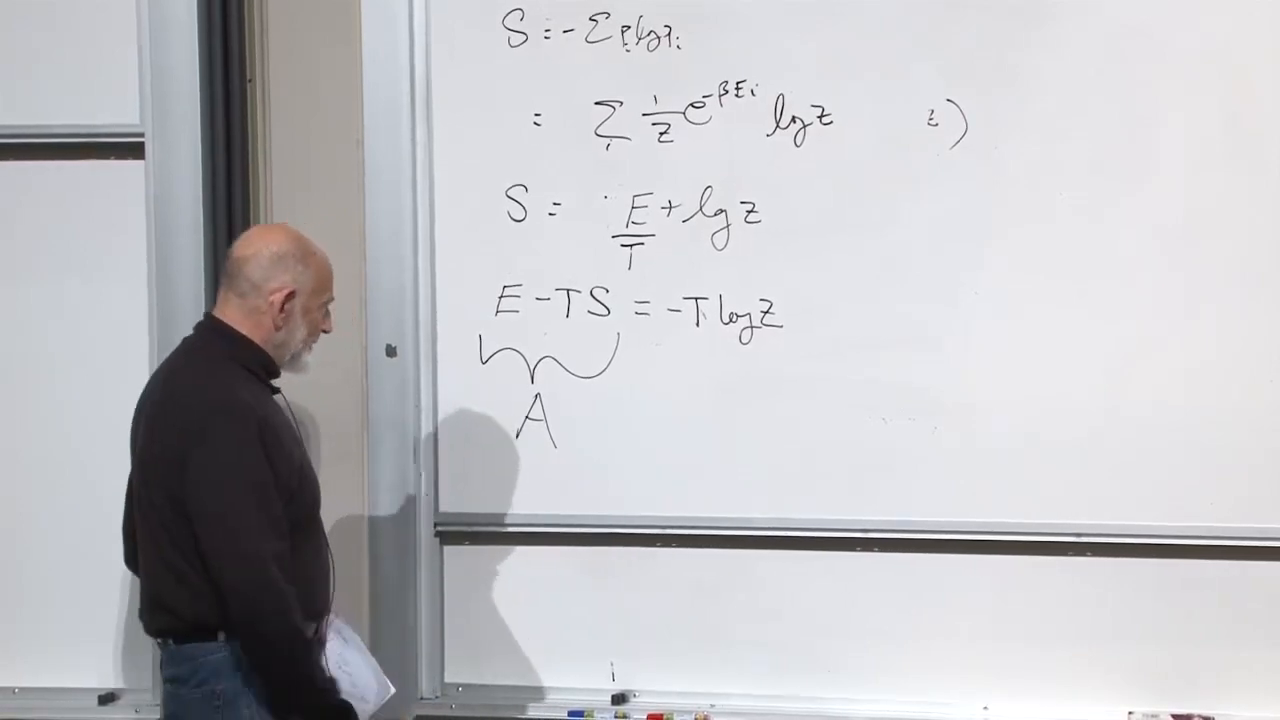
\includegraphics[width=0.90\textwidth]{lecture_05_figure_03.png}
\caption{正準エントロピー関係を\(A=E-TS=-T\log Z\)に整理したもの。}
\lectureframe{00:16:50}
\end{figure}

\section{制御パラメータとその応答}

制御パラメータとは、実験者が外部から変化させることができるマクロな量である。ピストンを動かすと、個々の分子を操作することなく体積が変化する。印加された電場や磁場も他の例である。より一般的なアンサンブルでは、粒子数も変化させることができる。

熱力学変数は自然に共役対をなす。体積は現在の問題における制御パラメータであり、圧力はその応答である。我々は\(V\)を変化させる。圧力は、系がその変化にエネルギー的にどのように抵抗するかを教えてくれる。後にエネルギーの微分がこの対を正確なものにする。

\begin{classroomqa}
\audiencequestion{圧力そのものを制御パラメータと見なせるだろうか。}
\lecturerresponse{外部圧力を固定する実験を設計することはできるが、ここで用いた構成ではピストンの位置が体積を固定し、内部圧力が応答である。圧力と体積は共役な変数であり、どちらが制御されるかはアンサンブルと装置に依存する。
\lecturetimestamp{00:19:22--00:20:01}}
\end{classroomqa}

\begin{classroomqa}
\audiencequestion{すべての分子は同一と仮定されるのか、それとも議論は気体に限られるのか。}
\lecturerresponse{熱力学の議論にはそのような制限は必要ない。シリンダーには複数の種、液体、あるいは圧縮される固体さえ入っていてよい。理想気体の分配関数は、一般的な圧力の式が確立された後に初めて特別な適用例となる。
\lecturetimestamp{00:20:02--00:20:39}}
\end{classroomqa}

\begin{classroomqa}
\audiencequestion{物質の量を別の外部操作として変化させられるだろうか。}
\lecturerresponse{はい。粒子数はもう一つの可能な制御パラメータである。それを動的に扱うと、それ自身の共役変数である化学ポテンシャルが導かれる。今夜の計算では、\(N\)は固定されたままである。
\lecturetimestamp{00:20:39--00:20:57}}
\end{classroomqa}

\begin{classroomqa}
\audiencequestion{液体の水と水蒸気が平衡状態で同時に存在できるだろうか。}
\lecturerresponse{共存温度と圧力においては存在できる。重力によって液体が蒸気の下に位置することがあるが、それでも二つの相は一つの温度を共有し、熱平衡を保つことができる。同じ一般的な統計力学の枠組みが適用される。
\lecturetimestamp{00:20:59--00:21:36}}
\end{classroomqa}

次の議論のために、エネルギーとエントロピーを二つの独立に調整可能な変数の従属関数と見なす：
\begin{equation}
 E=E(T,V),
 \qquad
 S=S(T,V).
 \label{eq:sm5-dependent-functions}
\end{equation}
温度と体積は熱力学状態空間上の座標を与える。エネルギーとエントロピーはその空間のすべての平衡点に数値を割り当てる。

\section{定エントロピー微分}

最終的に必要な微分は珍しいものである：
\[
 \left(\frac{\partial E}{\partial V}\right)_S.
\]
\(T\)と\(V\)は独立な座標であるが、この微分は従属関数\(S(T,V)\)を一定に保つよう制約しながら\(V\)を変化させることを求める。それは\((T,V)\)平面内の曲線に沿った微分であり、座標軸に沿ったものではない。

\begin{classroomqa}
\audiencequestion{後に微分\(dT/dV\)が用いられるのであれば、\(T\)と\(V\)はどのように独立でありうるのか。}
\lecturerresponse{それらは完全な状態空間上では独立である。制約\(S(T,V)=\mathrm{constant}\)を課すと、許される状態は一次元の等高線上に載る。その等高線に沿って、\(T\)は\(V\)の関数となり、その傾き\(dT/dV\)は well-defined である。
\lecturetimestamp{01:01:18--01:02:09}}
\end{classroomqa}

\begin{lemma}
\(E(T,V)\)と\(S(T,V)\)が微分可能であれば、\((\partial S/\partial T)_V\neq0\)であるところではどこでも
\begin{equation}
 \left(\frac{\partial E}{\partial V}\right)_S
 =
 \left(\frac{\partial E}{\partial V}\right)_T
 -
 \left(\frac{\partial E}{\partial S}\right)_V
 \left(\frac{\partial S}{\partial V}\right)_T.
 \label{eq:sm5-calculus-lemma}
\end{equation}
\end{lemma}

\begin{proof}
任意の無限小変位に対して、
\begin{equation}
 dE=
 \left(\frac{\partial E}{\partial V}\right)_T dV
 +
 \left(\frac{\partial E}{\partial T}\right)_V dT.
 \label{eq:sm5-total-differential-e}
\end{equation}
\(V\)を固定すると、連鎖律により\(S\)を中間変数として用いることができる：
\begin{equation}
 \left(\frac{\partial E}{\partial T}\right)_V
 =
 \left(\frac{\partial E}{\partial S}\right)_V
 \left(\frac{\partial S}{\partial T}\right)_V.
 \label{eq:sm5-chain-rule-e-s-t}
\end{equation}

ここで変位を\(S\)が一定である等高線に制限する。その等高線に沿って、
\begin{equation}
 0=dS=
 \left(\frac{\partial S}{\partial V}\right)_T dV
 +
 \left(\frac{\partial S}{\partial T}\right)_V dT.
 \label{eq:sm5-constant-entropy-differential}
\end{equation}
等高線の傾きについて解くと
\begin{equation}
 \left(\frac{dT}{dV}\right)_S
 =
 -
 \frac{\left(\frac{\partial S}{\partial V}\right)_T}
 {\left(\frac{\partial S}{\partial T}\right)_V}.
 \label{eq:sm5-entropy-contour-slope}
\end{equation}
\eqref{eq:sm5-total-differential-e}を\(dV\)で割り、
\eqref{eq:sm5-chain-rule-e-s-t}を用い、
\eqref{eq:sm5-entropy-contour-slope}を代入する：
\begin{align}
 \left(\frac{\partial E}{\partial V}\right)_S
 &=
 \left(\frac{\partial E}{\partial V}\right)_T
 +
 \left(\frac{\partial E}{\partial S}\right)_V
 \left(\frac{\partial S}{\partial T}\right)_V
 \left(\frac{dT}{dV}\right)_S \notag\\
 &=
 \left(\frac{\partial E}{\partial V}\right)_T
 -
 \left(\frac{\partial E}{\partial S}\right)_V
 \left(\frac{\partial S}{\partial V}\right)_T.
\end{align}
因子\((\partial S/\partial T)_V\)は相殺され、結果が証明される。
\end{proof}

\begin{figure}[t]
\centering
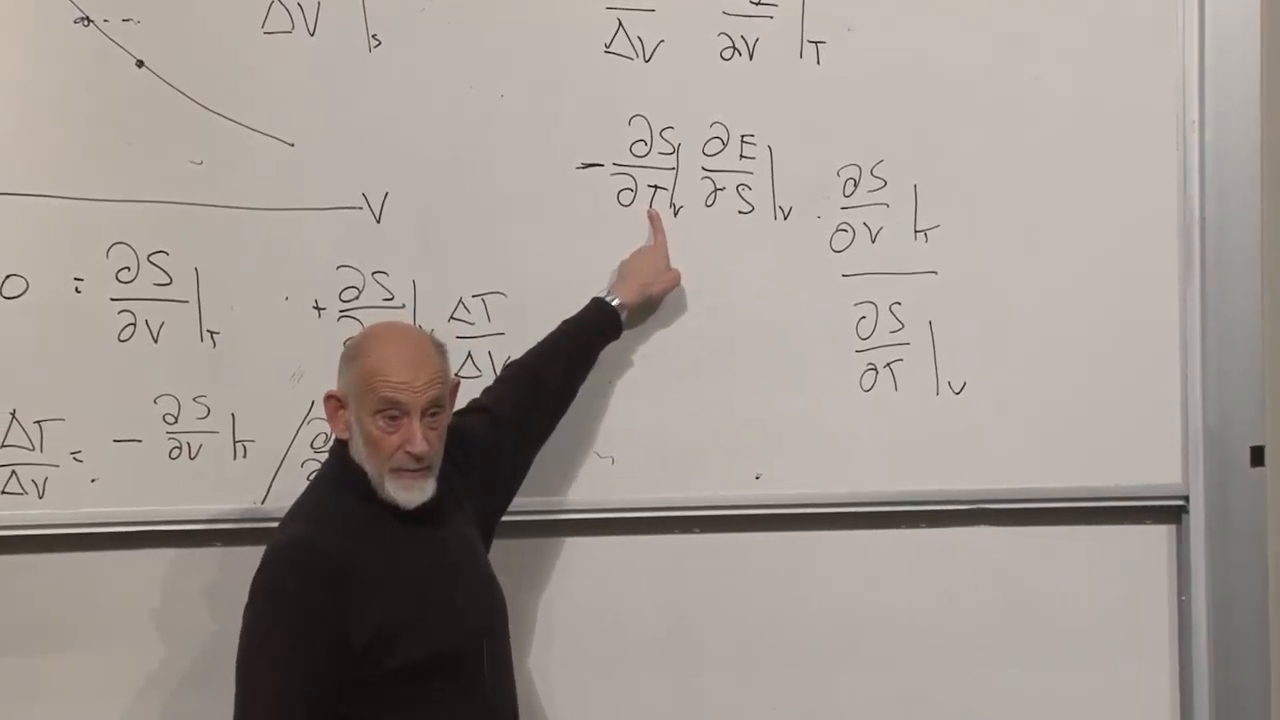
\includegraphics[width=0.90\textwidth]{lecture_05_figure_04.png}
\caption{微分補題を完成させる相殺における定エントロピー等高線の計算。}
\lectureframe{00:36:10}
\end{figure}

幾何学的な描像は装飾ではない。それは、一見奇妙な固定\(S\)微分が、独立な座標\(T\)と\(V\)における通常の偏微分で評価できる理由を説明する。構成の途中で\(\delta E/\delta V\)と書くことは、記号が指定された経路に沿った小さな変化の比を表すことを思い出させるのに有用である。

\begin{classroomqa}
\audiencequestion{\(dE\)の展開は単に偏微分の通常の定義ではないのか。}
\lecturerresponse{はい。全微分には特別なことは何も起こらない。唯一の追加要素は、後に等高線\(dS=0\)に制限することであり、それが\(dT\)と\(dV\)の関係を決定する。
\lecturetimestamp{00:29:26--00:29:32}}
\end{classroomqa}

\begin{classroomqa}
\audiencequestion{相殺には\((\partial S/\partial T)_V\)が非零であることが必要か。}
\lecturerresponse{はい。通常の安定な系では、
\[
 \left(\frac{\partial S}{\partial T}\right)_V
 =\frac{C_V}{T}>0,
\]
であるから、割り算は正当である。例外的な点には別途の注意が必要である。ハミルトニアンを固定すると、温度を上げることは正準エネルギー分布を広げ、通常はエントロピーを増加させる。温度を下げることはそれを狭める。これが単調性の議論の物理的に正しい向きである。
\lecturetimestamp{00:36:50--00:37:47}}
\end{classroomqa}

\section{ピストンの仕事と断熱条件}

ここで、この導関数に物理的な意味を与える。断面積\(\mathcal A\)のピストンを考える。これが外側へ\(dx\)だけ動くと、
\begin{equation}
 dV=\mathcal A\,dx.
 \label{eq:sm5-piston-volume}
\end{equation}
気体はピストンに力\(P\mathcal A\)を及ぼすので、気体がする仕事は
\begin{equation}
 \delta W_{\mathrm{by}}=P\mathcal A\,dx=P\,dV.
 \label{eq:sm5-piston-work}
\end{equation}
気体に熱が入らないなら、エネルギー保存により
\begin{equation}
 dE=-P\,dV.
 \label{eq:sm5-adiabatic-work}
\end{equation}
符号は物理的である。膨張の間、気体はピストンを押し上げるか加速し、自身のエネルギーは減少する。

\begin{figure}[t]
\centering
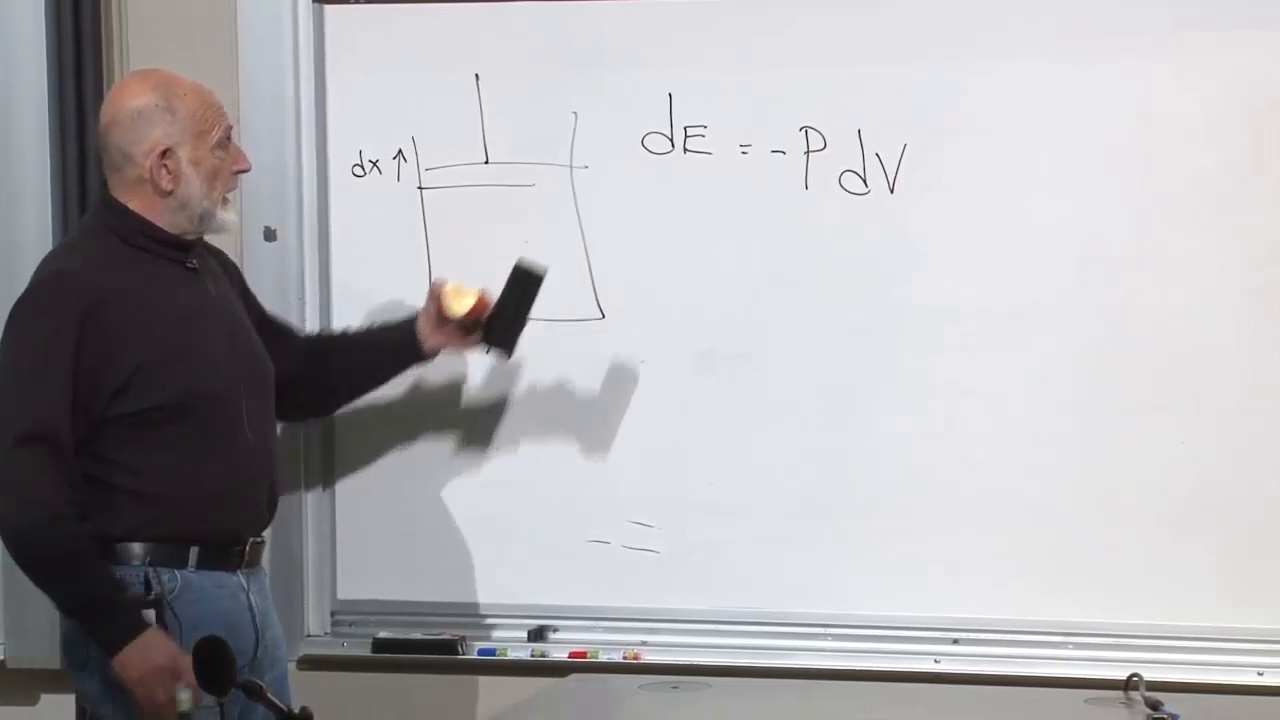
\includegraphics[width=0.90\textwidth]{lecture_05_figure_05.png}
\caption{ピストンの幾何と、完成した仕事の関係
\(dE=-P\,dV\)。}
\lectureframe{00:43:10}
\end{figure}

二つの条件が本質的である。ピストンは、系が平衡にいくらでも近いままでいられるほどゆっくり動かなければならず、また壁は断熱されていて、エネルギーが熱として供給されないようにしなければならない。急速な引き出しは、運動の間にどの分子も後退するピストンに到達しないほど速くなりうる。急速な圧縮は衝撃波を生じる。どちらの過程も、平衡状態の列では表されない。

\emph{断熱}という語は、熱移動がないことに対して使われることもあり、ゆっくりした変化に対して使われることもある。ここで要求される可逆過程では、両方の考えが入る。すなわち、変化は準静的かつ熱的に断熱されている。そのような条件下では、それは等エントロピーでもある。

\begin{classroomqa}
\audiencequestion{なぜ断熱変化はエントロピーを一定に保つのか。}
\lecturerresponse{系を量子力学的に見る。その多体エネルギー準位は体積に依存する。\(V\)がゆっくり変化するとき、断熱定理は各占有準位を、準位ラベル間の遷移なしに、連続的にその後継へ移す。エネルギー\(E_i(V)\)は動くが、占有確率\(p_i\)は固定されたままである。
\(S=-\sum_i p_i\log p_i\)はそれらの確率に依存するので、エントロピーは一定のままである。熱交換や不可逆な運動はこの結論を無効にするであろう。
\lecturetimestamp{00:43:37--00:49:15}}
\end{classroomqa}

\begin{figure}[t]
\centering
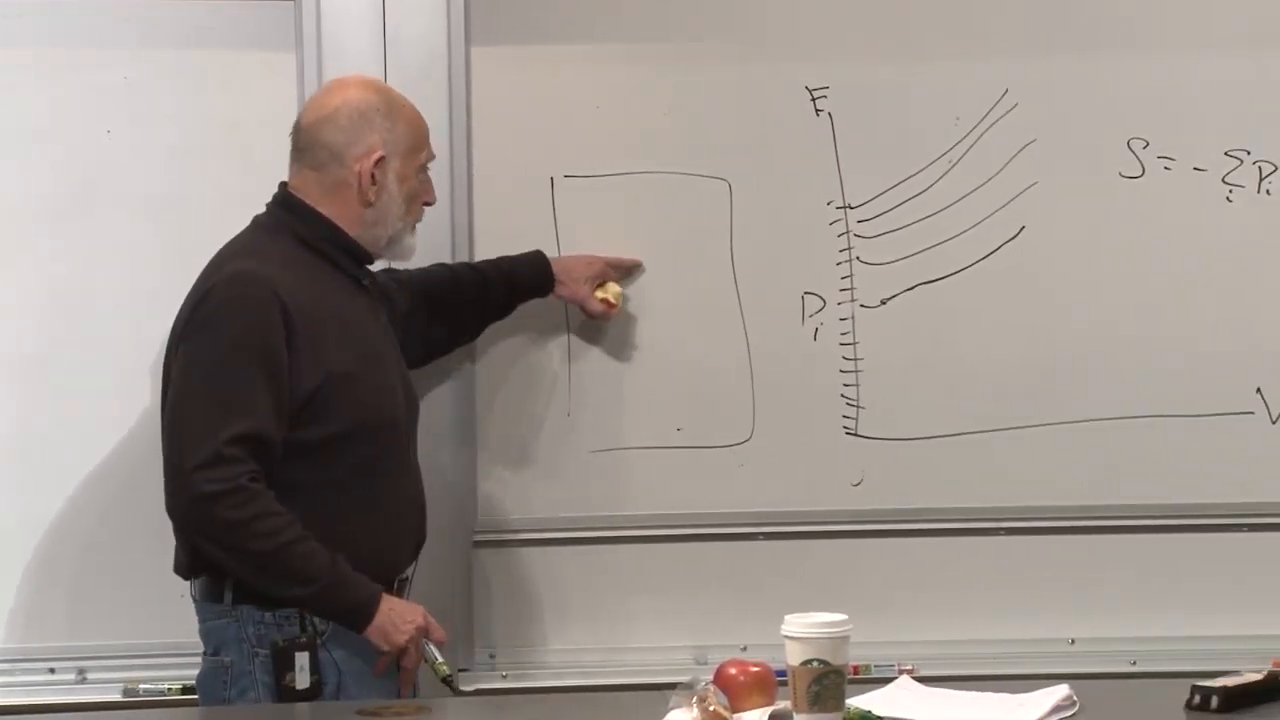
\includegraphics[width=0.90\textwidth]{lecture_05_figure_06.png}
\caption{多体エネルギー準位が体積とともに動く一方で、それらの占有確率は準位ラベルを保つ。}
\lectureframe{00:48:50}
\end{figure}

この一定エントロピーの経路に沿って評価された式\eqref{eq:sm5-adiabatic-work}は、圧力を
\begin{equation}
 P=-\left(\frac{\partial E}{\partial V}\right)_S.
 \label{eq:sm5-pressure-fixed-entropy}
\end{equation}
と同定する。これが圧力と体積の共役関係である。

\begin{classroomqa}
\audiencequestion{代わりにピストンを急速に動かすとどうなるか。}
\lecturerresponse{系は平衡を離れ、その詳細な力学が重要になる。突然の圧縮は衝撃を生じる。理想的な自由膨張では、どの分子もピストンに衝突する前にピストンが後退しうるので、仕事はなされず、体積が変化してもエネルギーは固定されたままである。気体は後に、増大したエントロピーとともに平衡へ緩和する。そのような過程は、
\eqref{eq:sm5-pressure-fixed-entropy}
における単一の平衡導関数では記述できない。
\lecturetimestamp{00:58:30--01:01:15}}
\end{classroomqa}

\begin{classroomqa}
\audiencequestion{変化がゆっくりであるかどうかを決める定量的条件は何か。}
\lecturerresponse{外部変化の時間は、関連する内部緩和時間に比べて長くなければならない。気体については、巨視的変化の間に多数の分子衝突と多数の壁への衝突が起こるべきである。正確な時間尺度は物質と幾何に依存するが、準静的極限そのものは一般的である。
\lecturetimestamp{01:02:09--01:03:20}}
\end{classroomqa}

\section{断熱エネルギーから分配関数へ}

物理的な式\eqref{eq:sm5-pressure-fixed-entropy}は、まだ計算しやすいものではない。正準統計力学は、\(T\)がボルツマン重みに直接現れるため、温度の関数を自然に与える。微積分の補題は、扱いにくい固定エントロピー導関数をその計算の言語へ変換する。
\begin{align}
 P
 &=
 -\left(\frac{\partial E}{\partial V}\right)_T
 +
 \left(\frac{\partial E}{\partial S}\right)_V
 \left(\frac{\partial S}{\partial V}\right)_T.
 \label{eq:sm5-pressure-lemma-substitution}
\end{align}
固定体積では、第一法則は\(dE=T\,dS\)を与えるので、
\begin{equation}
 \left(\frac{\partial E}{\partial S}\right)_V=T.
 \label{eq:sm5-e-s-temperature}
\end{equation}
したがって
\begin{equation}
 P=
 -\left(\frac{\partial E}{\partial V}\right)_T
 +
 T\left(\frac{\partial S}{\partial V}\right)_T.
 \label{eq:sm5-pressure-fixed-temperature-pieces}
\end{equation}

\begin{classroomqa}
\audiencequestion{圧力の式のマイナス符号はどこから来るのか。}
\lecturerresponse{それは気体がする仕事に由来する。
\(dE=-P\,dV\)（断熱膨張の間）。微積分の補題自体はその二つの項の間にマイナス符号をもつ。
\(P=-(\partial E/\partial V)_S\)
における全体のマイナスはそれら両方を反転させ、
\eqref{eq:sm5-pressure-fixed-temperature-pieces}
を生じる。
\lecturetimestamp{00:52:40--00:53:14}}
\end{classroomqa}

\(T\)は両方の導関数で固定されているので、
\begin{align}
 P
 &=
 -\left(\frac{\partial}{\partial V}(E-TS)\right)_T \notag\\
 &=
 -\left(\frac{\partial A}{\partial V}\right)_T.
 \label{eq:sm5-pressure-free-energy}
\end{align}
最後に\(A=-T\log Z\)を代入する。
\begin{equation}
 \boxed{
 P=
 T\left(\frac{\partial\log Z}{\partial V}\right)_T
 }.
 \label{eq:sm5-pressure-log-z}
\end{equation}

\begin{figure}[t]
\centering
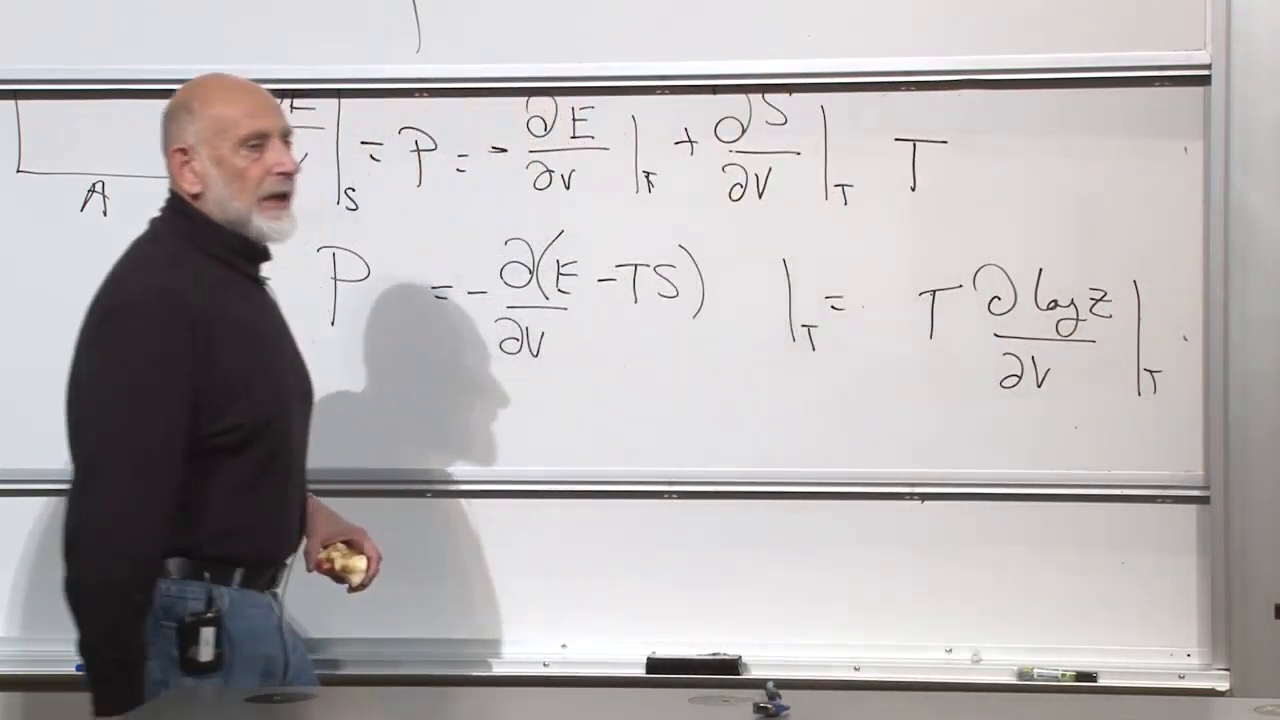
\includegraphics[width=0.90\textwidth]{lecture_05_figure_07.png}
\caption{引数の固定温度圧縮：
\(P=-(\partial A/\partial V)_T
=T(\partial\log Z/\partial V)_T\)。}
\lectureframe{00:55:55}
\end{figure}

\eqref{eq:sm5-pressure-log-z}のどこにも理想気体は仮定されていない。相互作用する流体、プラズマ、または固体について分配関数を計算できるなら、同じ導関数がその圧力を与える。より一般に、すべての外部制御パラメータは、適切な熱力学ポテンシャルを微分して得られる共役応答をもつ。分配関数はそのような応答を多数まとめ上げる。\(\log Z\)を\(\beta\)で微分するとエネルギーを与え、体積で微分すると圧力を与える。

\section{理想気体の状態方程式}

ここで初めて\(N\)個の非相互作用粒子の場合に限定する。古典的な相空間の規格化を保持したままだと、
\begin{equation}
 Z_N=
 \frac{1}{N!h^{3N}}
 \int d^{3N}q\,d^{3N}p\,
 \exp\!\left[
 -\beta\sum_{a=1}^{N}\frac{\mathbf p_a^2}{2m}
 \right].
 \label{eq:sm5-ideal-gas-partition-integral}
\end{equation}
位置座標が\(3N\)個、運動量座標が\(3N\)個ある。ハミルトニアンは位置に依存しないので、各粒子が容器の体積の因子を1つずつ寄与する：
\begin{equation}
 Z_N=
 \frac{V^N}{N!h^{3N}}I_p(\beta),
 \label{eq:sm5-ideal-gas-factorization}
\end{equation}
ここで運動量積分全体\(I_p(\beta)\)は\(V\)に依存しない。

\begin{classroomqa}
\audiencequestion{なぜ位置積分が\(3N\)個、運動量積分が\(3N\)個あるのか。}
\lecturerresponse{\(N\)個の粒子のそれぞれが3つの空間座標と3つの共役な運動量成分をもつ。その数は相空間の各半分で\(3N\)であり、\(N\)個の粒子にさらに\(3N\)個の粒子が加わるのではない。
\lecturetimestamp{01:04:19--01:04:28}}
\end{classroomqa}

対数をとると体積依存性が分離される：
\begin{equation}
 \log Z_N
 =
 N\log V-\log N!-3N\log h+\log I_p(\beta).
 \label{eq:sm5-log-ideal-gas-partition}
\end{equation}
因子\(1/N!\)、\(h^{-3N}\)、\(I_p(\beta)\)はすべて体積に依存しない。これらは絶対エントロピーやその他の問題には重要だが、この特定の導関数には重要でない。したがって
\begin{equation}
 \left(\frac{\partial\log Z_N}{\partial V}\right)_T
 =\frac{N}{V}.
 \label{eq:sm5-log-z-volume-derivative}
\end{equation}
式\eqref{eq:sm5-pressure-log-z}から直ちに
\begin{equation}
 P=\frac{NT}{V},
 \qquad
 \boxed{PV=NT}.
 \label{eq:sm5-ideal-gas-law}
\end{equation}が得られる。

\begin{classroomqa}
\audiencequestion{\(N\)はボルツマン分布を導出するのに用いたレプリカを依然として数えているのか。}
\lecturerresponse{いいえ。レプリカの構成は以前の導出における数え上げの道具であり、もはや存在しない。ここで\(N\)はこの1つの気体試料中の物理的粒子の数である。
\lecturetimestamp{01:07:38--01:08:05}}
\end{classroomqa}

数密度を
\begin{equation}
 \rho=\frac{N}{V}
 \label{eq:sm5-number-density}
\end{equation}
と定義すると、等価な形
\begin{equation}
 P=\rho T.
 \label{eq:sm5-density-equation-of-state}
\end{equation}が得られる。

\begin{classroomqa}
\audiencequestion{密度の形は\(N\)で割るのか、それとも\(V\)で割るのか。}
\lecturerresponse{\(PV=NT\)を\(V\)で割る：
\(P=(N/V)T=\rho T\)。ここで\(\rho\)は数密度であり、質量密度ではない。
\lecturetimestamp{01:08:45--01:09:16}}
\end{classroomqa}

\begin{figure}[t]
\centering
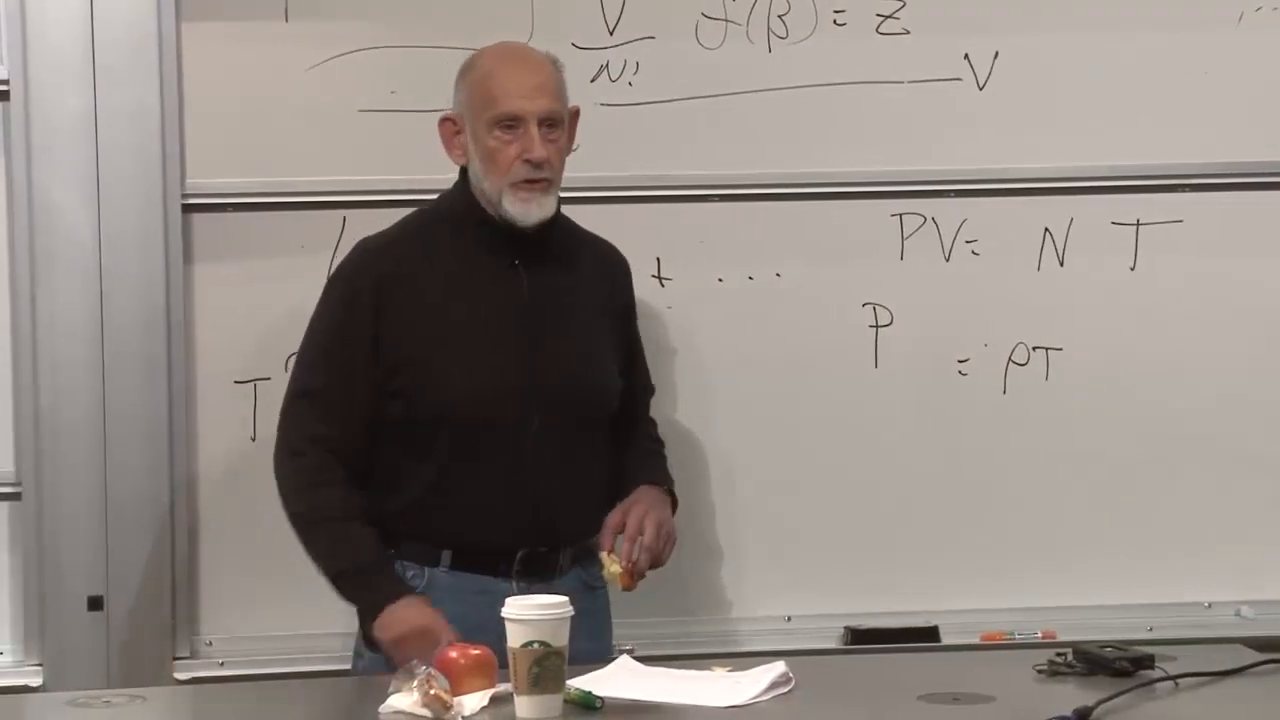
\includegraphics[width=0.90\textwidth]{lecture_05_figure_08.png}
\caption{\(\log Z\)の体積導関数と、それから得られる理想気体の状態方程式\(PV=NT\)、すなわち\(P=\rho T\)。}
\lectureframe{01:09:25}
\end{figure}

実験室温度\(T_K\)を復元すると、
\begin{equation}
 PV=Nk_BT_K.
 \label{eq:sm5-ideal-gas-law-laboratory}
\end{equation}
このよく知られた結果は運動論的な直観と一致するが、その導出は今や自由気体をはるかに超えて生き残る枠組みに基づいている。

\section{第二の配当：平衡揺らぎ}

圧力の計算は完了したが、約束した問いが1つ残っている：分配関数から他に何を引き出せるか。熱浴と熱接触している系を考える。そのエネルギーは固定されていない。エネルギーが出入りするので、繰り返しの測定はカノニカル平均の周りで揺らぐ。

\begin{classroomqa}
\audiencequestion{約束された揺らぎを今計算できるか。}
\lecturerresponse{はい。余分な時間によって同じ原理の第二の実演が可能になる：\(Z\)の導関数が測定可能な熱力学的情報を符号化している。
\lecturetimestamp{01:10:37--01:10:50}}
\end{classroomqa}

\subsection{分散と標準偏差}

\(\langle x\rangle=0\)をもつ確率変数\(x\)に対して、分布の幅の尺度は\(\langle x^2\rangle\)である。一般の分布に対しては、変数をその平均だけずらす：
\begin{equation}
 \delta x=x-\langle x\rangle.
 \label{eq:sm5-centered-variable}
\end{equation}
その平均は消え、
\begin{equation}
 \langle\delta x\rangle
 =
 \langle x\rangle-\langle x\rangle=0,
 \label{eq:sm5-centered-mean}
\end{equation}
その平均二乗は
\begin{align}
 (\Delta x)^2
 &\equiv
 \left\langle\left(x-\langle x\rangle\right)^2\right\rangle \notag\\
 &=
 \langle x^2\rangle
 -2\langle x\rangle^2
 +\langle x\rangle^2 \notag\\
 &=
 \langle x^2\rangle-\langle x\rangle^2.
 \label{eq:sm5-variance}
\end{align}
これが分散である。その正の平方根\(\Delta x\)が標準偏差である。

\begin{classroomqa}
\audiencequestion{なぜ
\(x-\langle x\rangle\)の平均がちょうどゼロなのか。}
\lecturerresponse{平均は線形であり、\(\langle x\rangle\)はすでに数である。したがって
\(\langle x-\langle x\rangle\rangle
=\langle x\rangle-\langle x\rangle=0\)。
\lecturetimestamp{01:14:02--01:14:22}}
\end{classroomqa}

\begin{classroomqa}
\audiencequestion{二乗揺らぎ、分散、二乗平均平方根幅、標準偏差の区別は何か。}
\lecturerresponse{分散は
\((\Delta x)^2=\langle x^2\rangle-\langle x\rangle^2\)。
標準偏差はその平方根\(\Delta x\)である。平均がゼロの変数では、標準偏差はその二乗平均平方根値でもある。
\lecturetimestamp{01:16:39--01:18:38}}
\end{classroomqa}

\begin{figure}[t]
\centering
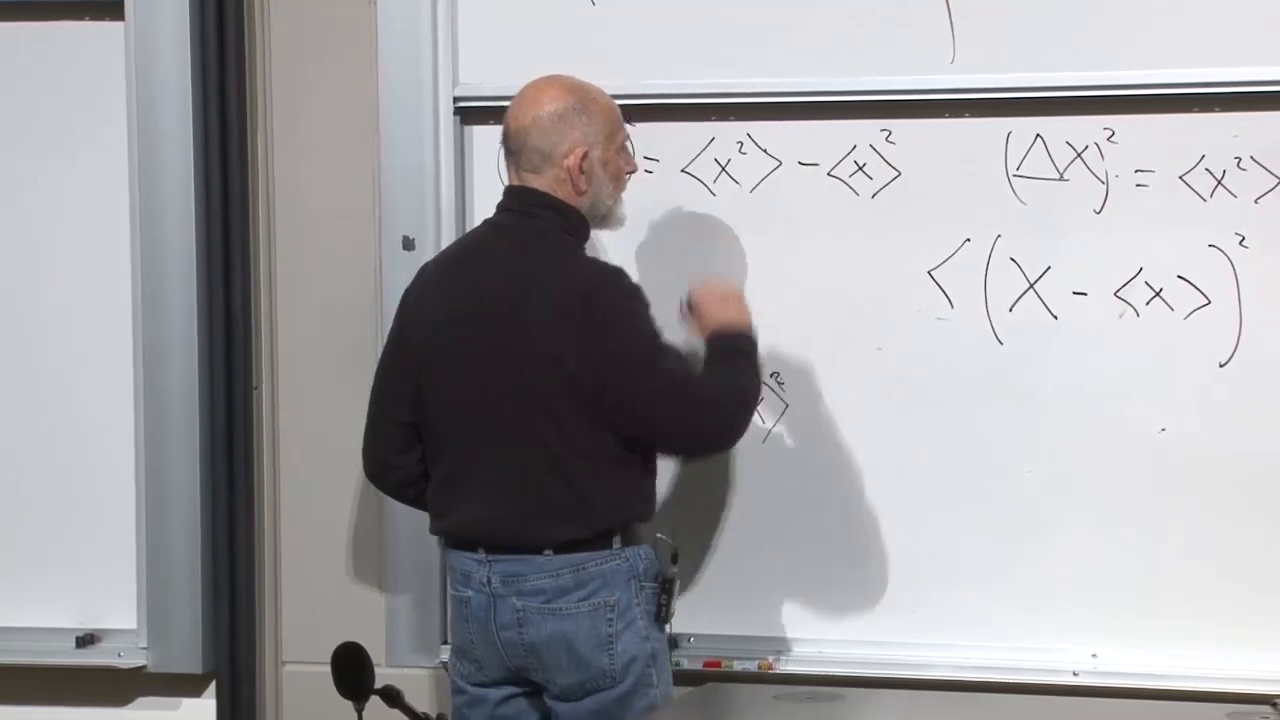
\includegraphics[width=0.90\textwidth]{lecture_05_figure_09.png}
\caption{ずらした変数と、\((\Delta x)^2=\langle x^2\rangle-\langle x\rangle^2\)を生み出す展開。}
\lectureframe{01:17:20}
\end{figure}

\subsection{分配関数からのエネルギーモーメント}

カノニカル集団では、
\begin{align}
 \langle E\rangle
 &=
 \frac{1}{Z}\sum_i E_i e^{-\beta E_i} \notag\\
 &=
 -\frac{1}{Z}\frac{\partial Z}{\partial\beta}
 =
 -\frac{\partial\log Z}{\partial\beta}.
 \label{eq:sm5-mean-energy-from-z}
\end{align}
\(E_i\)の因子1つ分の掛け算は、1つの負の\(\beta\)導関数によって生み出される。2階導関数は\(E_i^2\)を生成する：
\begin{equation}
 \langle E^2\rangle
 =
 \frac{1}{Z}\sum_i E_i^2e^{-\beta E_i}
 =
 \frac{1}{Z}\frac{\partial^2 Z}{\partial\beta^2}.
 \label{eq:sm5-second-energy-moment}
\end{equation}
したがってエネルギーの分散は
\begin{align}
 (\Delta E)^2
 &=
 \langle E^2\rangle-\langle E\rangle^2 \notag\\
 &=
 \frac{1}{Z}\frac{\partial^2Z}{\partial\beta^2}
 -
 \frac{1}{Z^2}
 \left(\frac{\partial Z}{\partial\beta}\right)^2 \notag\\
 &=
 \frac{\partial^2\log Z}{\partial\beta^2}
 =
 -\frac{\partial\langle E\rangle}{\partial\beta}.
 \label{eq:sm5-energy-variance-beta}
\end{align}
ここでもまた、複雑に見える観測量が\(\log Z\)の導関数になる。

\begin{figure}[t]
\centering
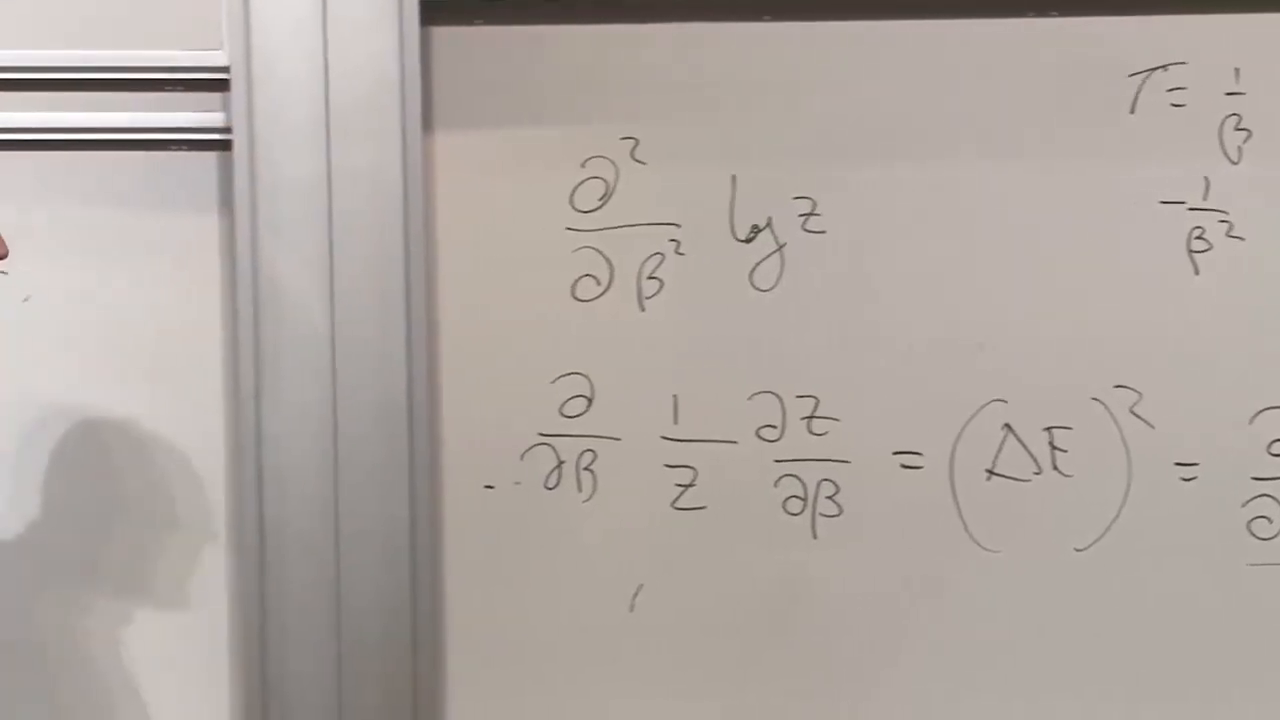
\includegraphics[width=0.90\textwidth]{lecture_05_figure_10.png}
\caption{\(\log Z\)の2階\(\beta\)導関数をエネルギーの分散と同定したもの。}
\lectureframe{01:29:00}
\end{figure}

\subsection{熱容量と揺らぎの大きさ}

講義単位では\(T=1/\beta\)なので、
\begin{equation}
 -\frac{\partial}{\partial\beta}
 =
 T^2\frac{\partial}{\partial T}.
 \label{eq:sm5-beta-temperature-derivative}
\end{equation}
体積を固定して、試料全体の熱容量を
\begin{equation}
 C_V\equiv
 \left(\frac{\partial\langle E\rangle}{\partial T}\right)_V.
 \label{eq:sm5-heat-capacity}
\end{equation}
と定義する。式\eqref{eq:sm5-energy-variance-beta}は
\begin{equation}
 \boxed{(\Delta E)^2=T^2C_V}
 \qquad (k_B=1).
 \label{eq:sm5-energy-fluctuation-lecture-units}
\end{equation}
となる。実験室温度\(T_K\)では、ここで
\(\beta=(k_BT_K)^{-1}\)、
\begin{equation}
 \boxed{(\Delta E)^2=k_BT_K^2C_V}.
 \label{eq:sm5-energy-fluctuation-laboratory}
\end{equation}

\begin{figure}[t]
\centering
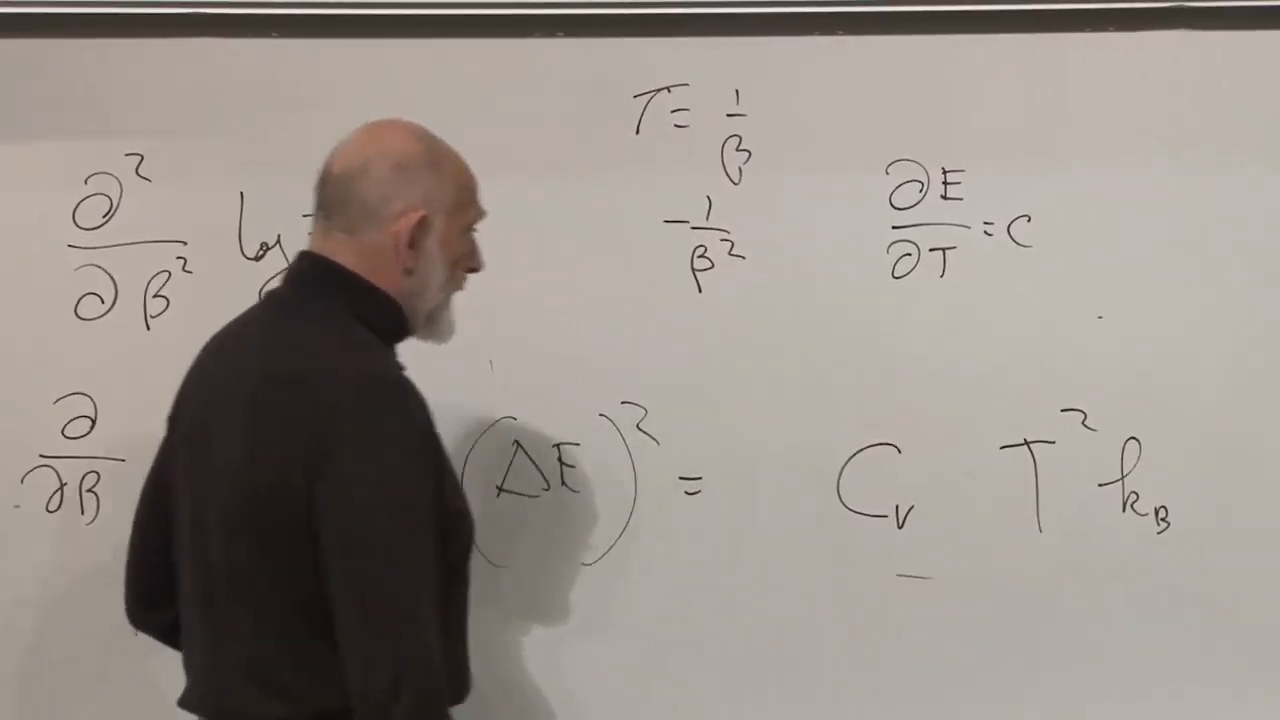
\includegraphics[width=0.90\textwidth]{lecture_05_figure_11.png}
\caption{\(\beta\) 微分から定積熱容量への変換。ただし、復元された \(k_B\) の因子を含む。}
\lectureframe{01:31:10}
\end{figure}

\begin{classroomqa}
\audiencequestion{微分は定圧ではなく定積を指定しなければならないのか。}
\lecturerresponse{はい。この正準分布による導出では、ハミルトニアンの外部制御パラメータを \(V\) を含めて固定したままにする。得られる量は \(C_V\) である。定圧アンサンブルでは体積と仕事が揺らぐことが許され、対応する熱力学ポテンシャルが必要となる。\eqref{eq:sm5-energy-fluctuation-laboratory} において \(C_V\) を単に \(C_P\) に置き換えることはできない。
\lecturetimestamp{01:29:01--01:29:28; 01:32:50--01:33:21}}
\end{classroomqa}

\begin{classroomqa}
\audiencequestion{\(C_V\) は物質定数か。}
\lecturerresponse{一般にはそうではない。温度、体積、相、組成に依存しうる。さらに、ここでの \(C_V\) は試料全体の熱容量であり、示量的である。比熱は質量、粒子数、または物質量で割って初めて得られる。
\lecturetimestamp{01:31:47--01:32:21; 01:33:23--01:34:55}}
\end{classroomqa}

通常の示量的な物質では、\(C_V\) は \(N\) に比例するので、\((\Delta E)^2\) は \(N\) に比例し、\(\Delta E\) は \(\sqrt{N}\) に比例する。平均エネルギー自体も \(N\) に比例する。したがって
\begin{equation}
 \frac{\Delta E}{\langle E\rangle}\sim\frac{1}{\sqrt{N}}.
 \label{eq:sm5-relative-fluctuation-scaling}
\end{equation}
巨視的な相対揺らぎはきわめて小さく、一方で微視的な試料ではそれが直接現れる。\eqref{eq:sm5-energy-fluctuation-laboratory} に \(k_B\) が現れることは、熱力学の観測量と分子の離散性とのこの結びつきを示しており、同等に、巨視的な単位をアボガドロ規模の計数に結びつけている。

圧力と揺らぎは今や同じ対象から現れた：
\[
 P=T\left(\frac{\partial\log Z}{\partial V}\right)_T,
 \qquad
 (\Delta E)^2=\frac{\partial^2\log Z}{\partial\beta^2}.
\]
これが中心的な教訓である。正しい拘束条件を特定しさえすれば、分配関数は単に確率を規格化するだけではない。その導関数が系の測定可能な熱力学を組織する。
\chapter{弱い相互作用、ビリアル補正、非完全微分}

\lectureoverview{まず測定と温度の操作的意味から始め、次に短距離相互作用が弱く加わったとき、希薄気体が理想気体の法則からどのようにずれるかを問う。分配関数はエネルギーと圧力への最初の相互作用補正を与え、その有効範囲を明らかにする。最後の数学的な補足では、完全微分、閉じたループ、および具体的な理想気体のテストを用いて、状態関数と経路に依存する熱および仕事を区別する。}

\section{計器が実際に測定するもの}

実験室の装置が直接自然の中に立ち入って抽象的な数学的変数を報告することはない。ばね秤は伸びを報告し、温度計は液柱の高さを報告する。我々が前者を力の測定、後者を温度の測定と呼ぶのは、目に見える応答と望ましい量との間に再現可能な関係が確立されているからにすぎない。

その関係には限られた範囲がある。ばねは弾性を保っている間だけフックの法則に従い、十分に大きな力はやがてそれを変形させ、あるいは破壊する。より一般に、滑らかな読み取り値\(R\)が物理変数\(X\)に依存するならば、選ばれた動作点\begin{equation}
 \Delta R \simeq
 \left.\frac{dR}{dX}\right|_{X_0}\Delta X.
 \label{eq:sm6-local-linear-response}
\end{equation}の近くで、読み取り値の小さな変化は、たとえ全応答曲線が非線形であっても、対象変数の小さな変化に比例する。この局所線形化が校正の通常の論理である。

読み取り値は厄介な変数にも依存しうる。ばねは温度や圧力に弱く応答することがある。温度計の水銀の高さは、重力を通じて向きに、ガラスの性質に、あるいは材料の緩やかな変化に応答しうる。測定プロトコルはこれらの依存性が存在しないことを証明するのではなく、それらを固定し、あるいは要求される尺度で無視できることを示すのである。

\begin{classroomqa}
\audiencequestion{局所的な重力場、あるいは温度計を保持する向きが読みを変えうるだろうか。}
\lecturerresponse{原理的には変わりうる。向きが無視できない効果を持つならば、温度計を鉛直に保持せよという指示が計器の定義の一部となる。地球表面付近では重力場は十分に安定しているので、残る変動は通常無視できる。
\lecturetimestamp{00:04:08--00:05:00}}
\end{classroomqa}

\begin{classroomqa}
\audiencequestion{経年変化や化学変化が校正を徐々に変えうるだろうか。}
\lecturerresponse{変わりうる。水銀とガラスは通常の測定には十分不活性であり、途方もなく長い時間尺度での変化は実験にとって無関係である。校正は常に、特定の計器、範囲、プロトコル、および期間についての言明である。
\lecturetimestamp{00:05:03--00:06:11}}
\end{classroomqa}

摂氏温度計では、二つの再現可能な基準状態が便利な目盛りを与える。\(h_f\)と\(h_b\)がそれぞれ水の凝固点と沸点における液柱の高さであるならば、応答がほぼ線形である範囲内で、
\begin{equation}
 T_{\mathrm C}=100\,\frac{h-h_f}{h_b-h_f}.
 \label{eq:sm6-celsius-calibration}
\end{equation}
凝固点で\(T_{\mathrm C}=0\)とする選択は慣習によるものである。それは熱エネルギーがゼロの状態ではなく、冬のある日の華氏零度が絶対零度でないのと同じである。

\begin{figure}[t]
\centering
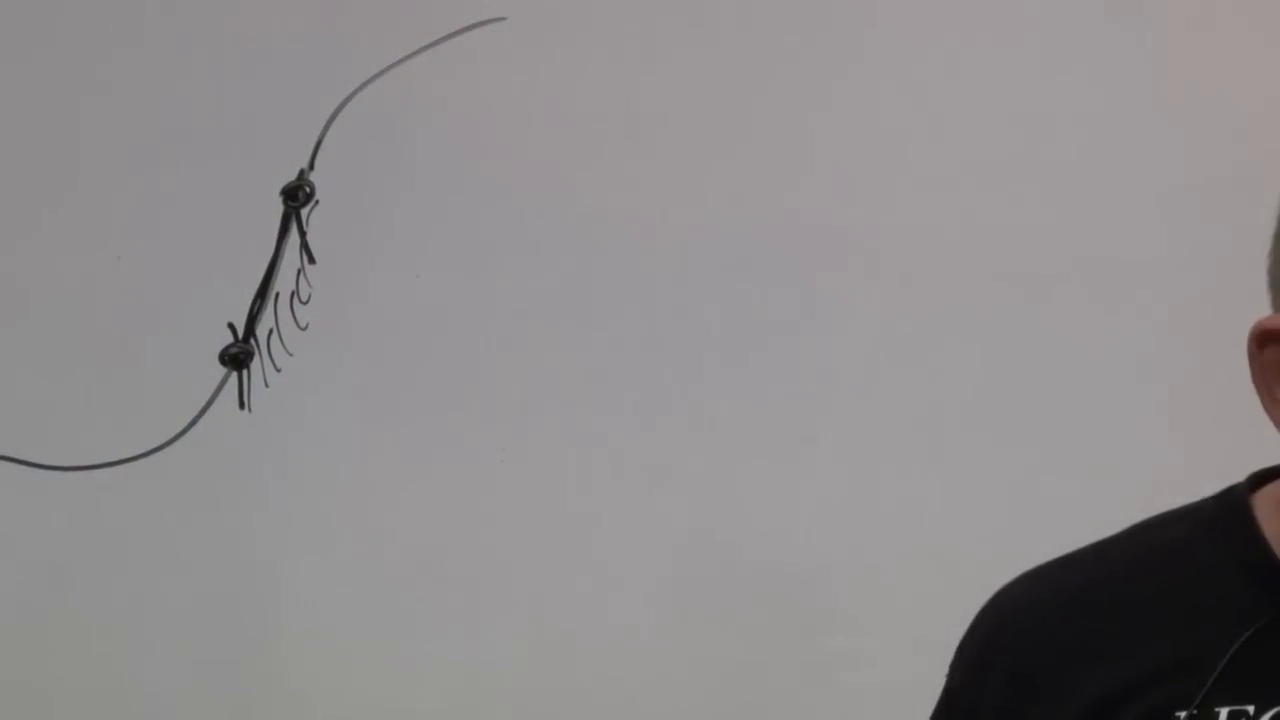
\includegraphics[width=0.90\textwidth]{lecture_06_figure_03.png}
\caption{滑らかだが非線形な温度計の応答。線形校正のために短い区間が区切られている。}
\lectureframe{00:07:55}
\end{figure}

\section{平衡とエネルギー尺度としての温度}

温度計は、温度計と近傍の媒質が熱平衡に達した後に初めて、その周囲の温度を測定する。それ以前は、その読みは単に平衡に向かって変化しているにすぎない。実用的なテストは初等的である。読みが変化しなくなるまで待てばよい。その規則の単純さは、待ち時間を決める物理過程を隠している。

\begin{classroomqa}
\audiencequestion{平衡化は球部の周りの境界層のみに関わるのか、またどれだけ待つべきか。}
\lecturerresponse{エネルギーはガラスを横切り、周囲の媒質と交換されねばならないので、時間は温度計、その熱伝導率、および媒質に依存する。直接の周囲もまた、一様な平衡状態を代表していなければならない。実験的には、読みが漂わなくなったときに受け入れられる。
\lecturetimestamp{00:08:45--00:10:13}}
\end{classroomqa}

この待ち時間において、温度と密度は異なる役割を果たす。非常に希薄な気体は非常に高温でありうる。存在する少数の分子は大きな運動エネルギーを担いうる。しかしそれらの分子は温度計にまれにしか衝突しないので、平衡化は遅くなりうる。温度を固定したまま密度を百倍あるいは千倍下げても、分子のエネルギー尺度は下がらない。それはそのエネルギーが計器に伝達される速さを下げるのである。

\begin{classroomqa}
\audiencequestion{室内の放射は空気とは異なる温度をもちうるか。}
\lecturerresponse{はい。物質と放射が一つの温度を共有するのは、両者が互いに熱平衡にあるときだけである。照明された室内では、中性の空気は多くの光学的放射と弱くしか結合せず、光子集団は空気の温度における平衡黒体場である必要はない。
\lecturetimestamp{00:11:26--00:12:20}}
\end{classroomqa}

いったん平衡が成立すれば、温度はエネルギー尺度とみなすのが最もよい。我々は引き続き\(k_B=1\)となる単位を用いるので、\(T\)自身がエネルギーの次元をもつ。単原子理想気体では、
\begin{equation}
 E_0=\frac{3}{2}NT.
 \label{eq:sm6-ideal-energy}
\end{equation}
分子あたりの熱エネルギーは\(T\)によって定まるが、対応する速さは依然として分子質量に依存する。

\section{弱い相互作用を入れる}

\begin{classroomqa}
\audiencequestion{理想気体近似はどのような条件で破綻し、その破綻を数学的に示せるか。}
\lecturerresponse{解けた非相互作用気体から出発し、小さな相互作用を入れる。その変化について展開し、第一補正を計算し、それを理想項と比較する。補正がもはや小さくなくなるとき、近似は破綻する。
\lecturetimestamp{00:12:25--00:14:40}}
\end{classroomqa}

これが標準的な摂動の戦略である。問題が\(\lambda=0\)で可解ならば、結合\(\lambda\)を導入して
\begin{equation}
 F(\lambda)=F(0)+\lambda F_1+\lambda^2F_2+\cdots,
 \label{eq:sm6-perturbative-template}
\end{equation}
と書き、保持した各項がその前の項より小さいかどうかを問う。ここで参照問題は理想気体である。物理的な小ささは、希薄な試料、平均間隔に比べて短い相互作用距離、そして第一の相互作用項が有用となる程度に弱いポテンシャルから生じる。高密度や長距離力は、個々の出会いが穏やかに見えても近似を無効にしうる。

\(x_i\in\mathbb R^3\)と\(p_i\in\mathbb R^3\)を分子\(i\)の位置と運動量とする。質量\(m\)の同種分子に対して、
\begin{equation}
 H(X,P)=
 \sum_{i=1}^{N}\frac{p_i^2}{2m}
 +\sum_{i<j}u\!\left(|x_i-x_j|\right),
 \label{eq:sm6-interacting-hamiltonian}
\end{equation}
をとる。ここで\(X=(x_1,\ldots,x_N)\)、\(P=(p_1,\ldots,p_N)\)である。制限\(i<j\)は自己対を除き、\((i,j)\)を一度だけ数える：
\begin{equation}
 \sum_{i<j}1=\binom{N}{2}=\frac{N(N-1)}{2}.
 \label{eq:sm6-pair-count}
\end{equation}

\begin{classroomqa}
\audiencequestion{なぜ両方の粒子ラベルについて独立に和をとらないのか。}
\lecturerresponse{対\((3,7)\)は\((7,3)\)と同じ物理的対であり、粒子は自分自身と対にならない。和を\(i<j\)に制限することはこの二つの事実を強制する。質量の記号は\(m\)のまま保ち、一方で\(i,j\)は粒子を表す。これは\(m\)が両方の目的に用いられるときに生じうる記法の衝突を避けるためである。
\lecturetimestamp{00:17:52--00:19:12}}
\end{classroomqa}

全配置ポテンシャルを
\begin{equation}
 U(X)=\sum_{i<j}u\!\left(|x_i-x_j|\right).
 \label{eq:sm6-total-potential}
\end{equation}
と書く。相互作用は並進不変かつ短距離であると仮定する：\(r\)が分子の長さに比べて大きいとき、\(u(r)\)は無視できるようになる。

\section{積分された対の強さ}

弱い対ポテンシャルの積分が一つだけ第一補正に入る：
\begin{equation}
 U_0\equiv\int_{\mathbb R^3}d^3r\,u(r).
 \label{eq:sm6-u0-definition}
\end{equation}
その単位はエネルギー掛ける体積である。これは相互作用の典型的な強さと、その相互作用が有意である体積とを組み合わせたものである。

\begin{figure}[t]
\centering
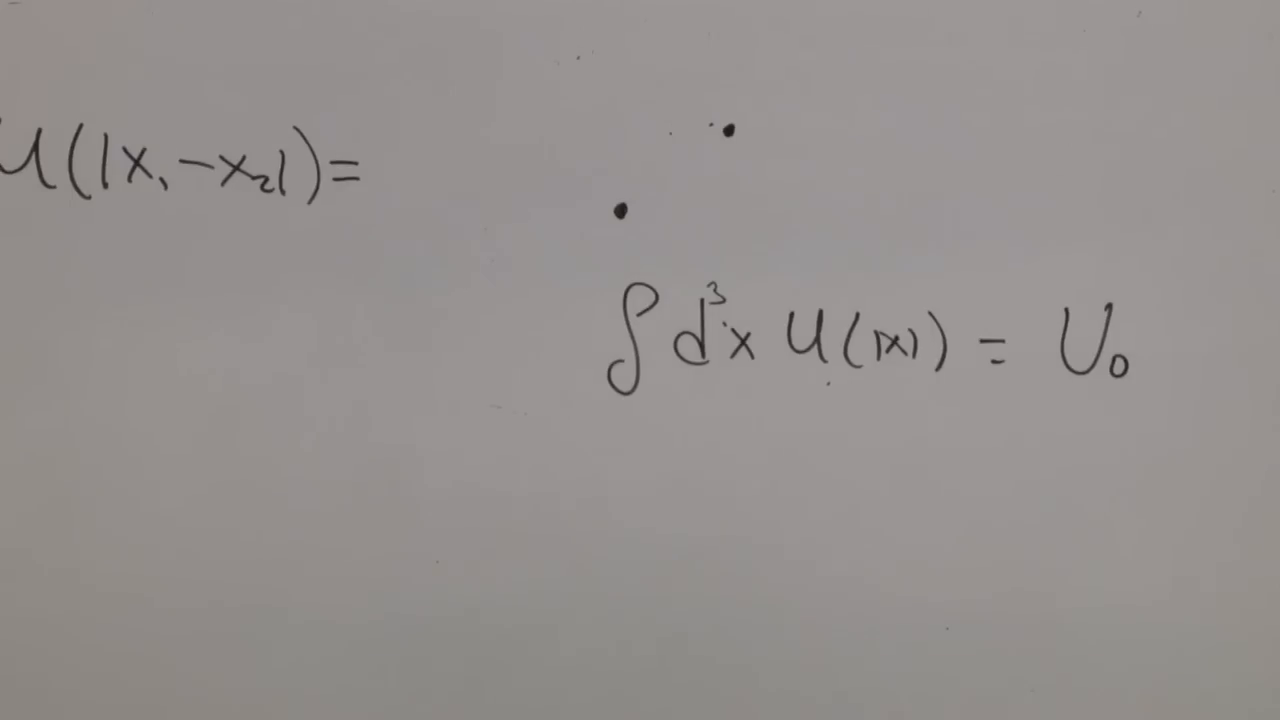
\includegraphics[width=0.90\textwidth]{lecture_06_figure_04.png}
\caption{短距離対ポテンシャルを積分された強さ\(U_0=\int d^3r\,u(r)\)に圧縮したもの。}
\lectureframe{00:25:15}
\end{figure}

\(U_0\)がなぜ有用かを知るために、一つの対を考える：
\begin{equation}
 I_2=\int_V d^3x_1\,d^3x_2\,
 u\!\left(|x_1-x_2|\right).
 \label{eq:sm6-two-particle-integral}
\end{equation}
相対座標\(r=x_2-x_1\)を導入する。境界から離れて、相対積分は\(U_0\)を与え、一方で対の共通位置は容器全体を動く。したがって
\begin{equation}
 I_2=V U_0+\text{surface corrections}.
 \label{eq:sm6-pair-integral-vu0}
\end{equation}
補正は、壁から一相互作用距離以内にある粒子から生じ、そこでは相対座標の近傍の一部が箱の外にある。その相対的な重要度は表面対体積の比としてスケールし、巨視的極限で消える。

\begin{classroomqa}
\audiencequestion{\(U_0\)は一つの選ばれた対を指すのか、そして一方の粒子は他方から固定された間隔に保たれるのか。}
\lecturerresponse{それは任意の一対に対する共通の相互作用則を指す。第一の粒子を固定し、第二の粒子をあらゆる相対位置について積分する。この積分の間、間隔は固定されていない。近傍の相互作用領域だけが有意に寄与し、\(U_0\)を生じる。
\lecturetimestamp{00:26:03--00:27:33}}
\end{classroomqa}

\begin{classroomqa}
\audiencequestion{なぜ第二の位置積分は容器全体の体積を与えるのに、第一のそれは与えないのか。}
\lecturerresponse{相対配置が\(U_0\)に積分された後、対全体は試料中を並進しうる。その共通の並進が大きな因子\(V\)を与える。相互作用近傍はすでに\(U_0\)の内部に含まれる分子スケールの体積であり、容器体積に等しい別の因子ではない。
\lecturetimestamp{00:27:48--00:29:21}}
\end{classroomqa}

\begin{classroomqa}
\audiencequestion{値はどの点を固定するかに依存しうるか、特に壁の近くではどうか。}
\lecturerresponse{並進不変性により、バルクの値は固定点に依存しない。壁の近くでは、隣接するいくつかの位置が利用できないため、積分はわずかに異なる。影響を受けるのは分子程度の厚さの表面層だけなので、箱が巨視的であれば誤差は無視できる。
\lecturetimestamp{00:29:24--00:31:22}}
\end{classroomqa}

\begin{classroomqa}
\audiencequestion{結果はすべての二粒子配置にわたって積分したポテンシャルエネルギーであり、なぜ一つの大きな体積にのみ比例するのか。}
\lecturerresponse{はい。その単位はエネルギー×体積の二乗である。なぜなら\(V U_0\)は一つの容器体積と一つの分子相互作用体積を含むからである。そのうち試料の大きさとともに増大するのは前者だけである。
\lecturetimestamp{00:31:31--00:32:04}}
\end{classroomqa}

\begin{classroomqa}
\audiencequestion{一定体積で面積を最小にする球を選ぶことは、バルクの答えを変えるか。}
\lecturerresponse{変わるのは小さな境界補正だけである。通常の巨視的な形状では、表面から分子距離以内にある粒子の数は、バルク内の粒子の数に比べて無視できる。表面が重要になるのは、容器自体が分子スケールに近づく場合だけである。
\lecturetimestamp{00:32:04--00:33:58}}
\end{classroomqa}

\begin{classroomqa}
\audiencequestion{粒子の軌道をポテンシャルに置き換えることで、衝突は省略されたのか。}
\lecturerresponse{いいえ。力はポテンシャルの導関数であり、まさに衝突を生み出すものである。平衡統計力学では、それらの衝突を一つ一つ追う必要はない。その効果はエネルギーに、したがってボルツマン重みに符号化されている。
\lecturetimestamp{00:33:59--00:35:29}}
\end{classroomqa}

\begin{classroomqa}
\audiencequestion{対力を保持しつつ真の三体相互作用を保持しないことで、何が失われるか。}
\lecturerresponse{微視的エネルギーは真の三体項を含みうるし、対ポテンシャルの高次項も多粒子相関を生み出す。しかし希薄気体中では、指定された三つの粒子が一つの分子近傍を占める確率は、二つの場合よりはるかに低い。したがって対効果が第一の密度補正を与え、より高次のクラスターは密度のより高い冪で寄与する。
\lecturetimestamp{00:35:29--00:38:14}}
\end{classroomqa}

\section{自動操縦での分配関数}

統計的手法の利点がここで見えてくる。ハミルトニアンが指定されれば、壁の近くや衝突中における詳細な速度分布を推測する必要はない。正準分配関数を書き下し、その代数をたどればよい。
\begin{equation}
\begin{aligned}
 Z&=
 \frac{1}{N!h^{3N}}
 \int d^{3N}P\,d^{3N}X\\
 &\qquad{}\times e^{-\beta K(P)}e^{-\beta U(X)},\\
 K(P)&=\sum_i\frac{p_i^2}{2m}.
\end{aligned}
 \label{eq:sm6-full-partition-function}
\end{equation}
因子\(h^{3N}\)は古典的位相空間の測度を無次元にし、\(N!\)は同種粒子の置換による過剰計数を取り除く。

\begin{figure}[t]
\centering
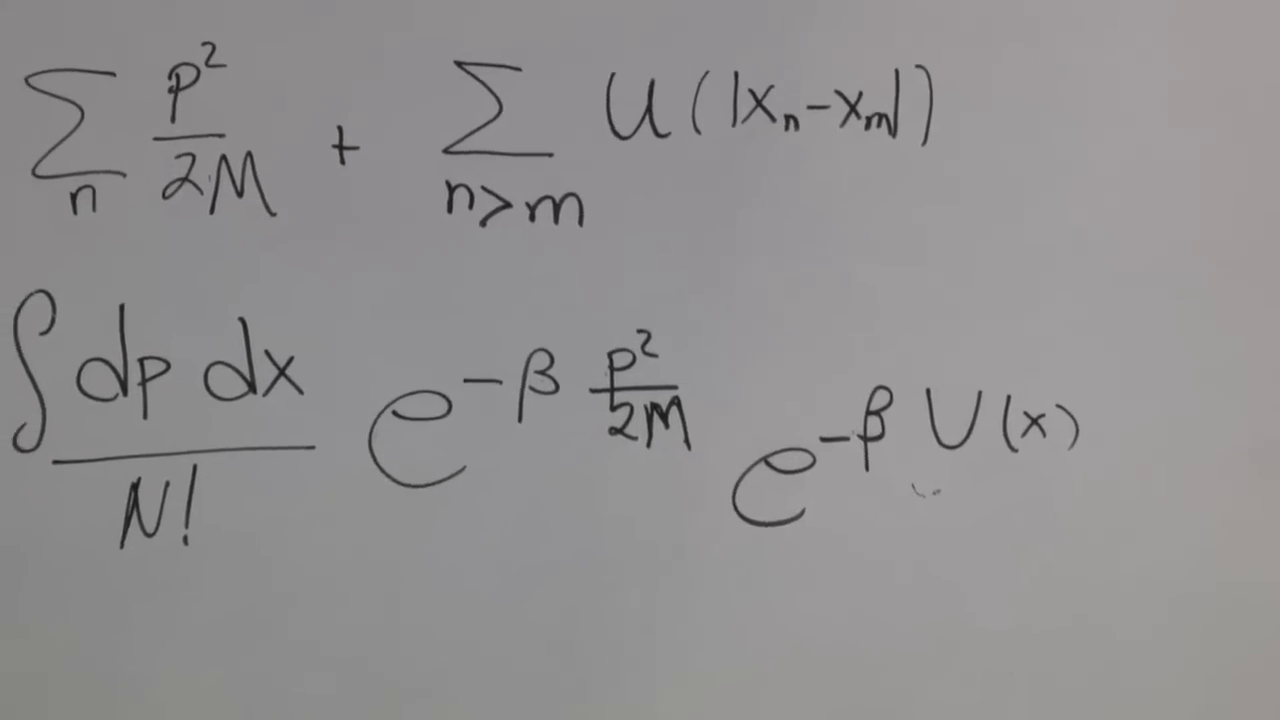
\includegraphics[width=0.90\textwidth]{lecture_06_figure_05.png}
\caption{多粒子エネルギーと、分配関数における対応する運動および配置の因子。}
\lectureframe{00:40:35}
\end{figure}

運動量と位置が分離する。配置積分に\(V^N\)を掛けて割ることで、理想気体の結果が分離される。
\begin{align}
 Z
 &=\left[
 \frac{V^N}{N!h^{3N}}
 \int d^{3N}P\,e^{-\beta K(P)}
 \right] \notag\\
 &\quad\times\left[
 \frac{1}{V^N}
 \int d^{3N}X\,e^{-\beta U(X)}
 \right] \notag\\
 &\equiv Z_0\,C(\beta,V,N).
 \label{eq:sm6-z-factorization}
\end{align}
おなじみのガウス因子は
\begin{equation}
 \int d^{3N}P\,e^{-\beta K(P)}
 =\left(\frac{2\pi m}{\beta}\right)^{3N/2}.
 \label{eq:sm6-gaussian-factor}
\end{equation}

\begin{figure}[t]
\centering
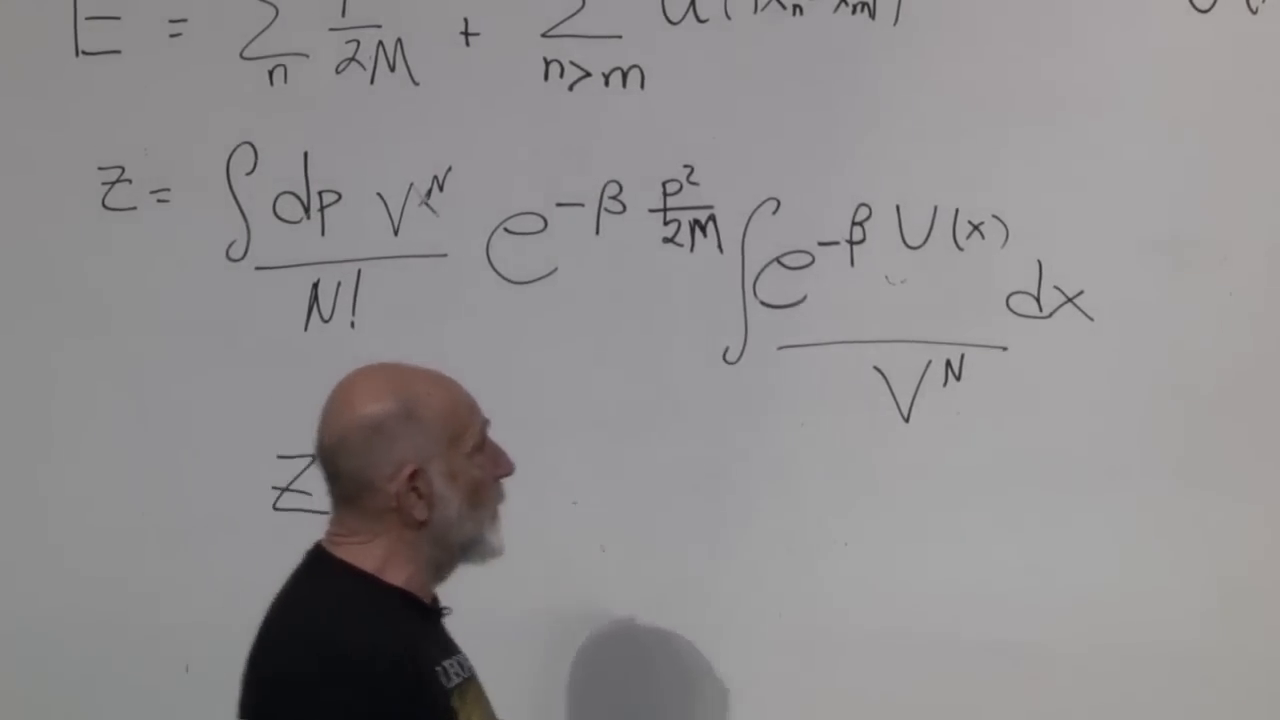
\includegraphics[width=0.90\textwidth]{lecture_06_figure_06.png}
\caption{規格化された配置因子から分離された理想気体の分配関数。}
\lectureframe{00:43:45}
\end{figure}

\(N!\)因子は規格化された比\(C\)にも、以下で用いる特定の固定\(N\)微分にも影響しないが、熱力学全体からは不要ではない。正しい状態の数え上げと示量的エントロピーにとって不可欠である。

相互作用の一次までで、
\begin{equation}
 e^{-\beta U(X)}
 =1-\beta U(X)+O(U^2).
 \label{eq:sm6-boltzmann-expansion}
\end{equation}
したがって、
\begin{align}
 C
 &=
 1-\frac{\beta}{V^N}
 \sum_{i<j}
 \int d^{3N}X\,u(|x_i-x_j|)
 +O(U^2) \notag\\
 &=
 1-\frac{\beta}{V^N}
 \frac{N(N-1)}{2}
 V^{N-2}(V U_0)+O(U^2) \notag\\
 &=
 1-\beta\frac{N(N-1)}{2V}U_0+O(U^2).
 \label{eq:sm6-configurational-correction}
\end{align}
各対は同じ\emph{積分}をもつのであり、同じ瞬間的な分離やポテンシャルエネルギーをもつのではない。残りの\(N-2\)個の位置積分はそれぞれ\(V\)の因子を一つ寄与する。

\begin{figure}[t]
\centering
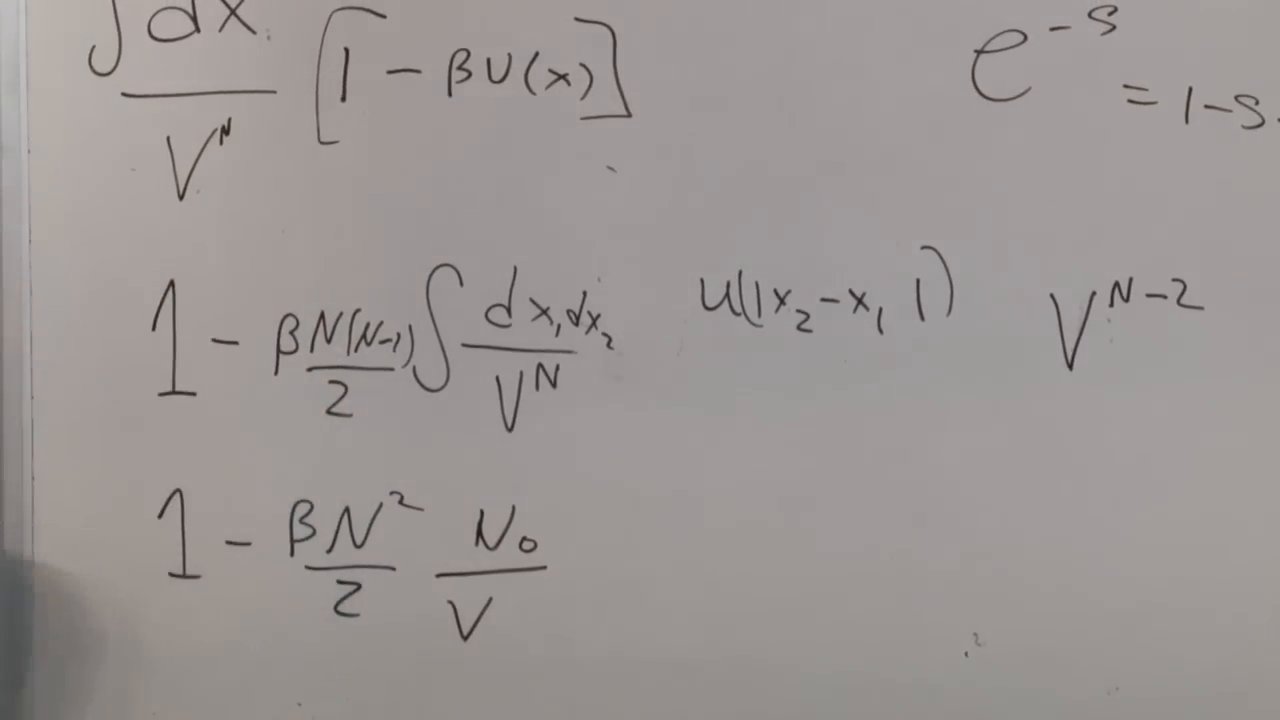
\includegraphics[width=0.90\textwidth]{lecture_06_figure_07.png}
\caption{対の数え上げ、傍観座標の体積、および第一の配置補正\(1-\beta N^2U_0/(2V)\)。}
\lectureframe{00:53:40}
\end{figure}

\begin{classroomqa}
\audiencequestion{主要な\(1\)は、分離ゼロでポテンシャルが消えることを仮定しているのか。}
\lecturerresponse{いいえ。それは指数級数のゼロ次項であり、\(u(0)\)の値に依存しない。ポテンシャルは次の項\(-\beta U(X)\)に入る。
\lecturetimestamp{00:46:19--00:46:48}}
\end{classroomqa}

\begin{classroomqa}
\audiencequestion{異なる対が異なる分離をもつのに、なぜすべての対を同じ式で置き換えてよいのか。}
\lecturerresponse{それらの点ごとの値が等しいとされているのではない。各項は同じ完全な配置空間にわたって積分され、粒子ラベルは一つの対を別の対から区別しない。積分は同一の形と同一の値をもつ。
\lecturetimestamp{00:50:00--00:51:07}}
\end{classroomqa}

\begin{classroomqa}
\audiencequestion{対の数は\(N(N-1)/2\)か、それとも
\(N(N+1)/2\)か。}
\lecturerresponse{\(N(N-1)/2\)である。一つの粒子を選んだ後には
\(N-1\)個の異なる相手しかなく、2で割ることで逆順の
順序が除かれる。巨視的な\(N\)では、\(N(N-1)\)を\(N^2\)に置き換えても
相対的な\(1/N\)の補正しか変わらない。
\lecturetimestamp{00:48:33--00:49:56}}
\end{classroomqa}

\(\log(1-x)=-x-x^2/2-x^3/3-\cdots\)は交代級数ではないので、
一次の対数は
\begin{equation}
 \log Z
 =
 \log Z_0
 -\beta\frac{N(N-1)}{2V}U_0
 +O(U^2).
 \label{eq:sm6-logz-correction}
\end{equation}
である。大きな\(N\)では、\(N(N-1)\)を\(N^2\)に置き換えてよく、そこでは有限の\(N\)による区別は必要ない。

\begin{remark}
制御された低密度の定式化では、Mayer関数
\(f(r)=e^{-\beta u(r)}-1\)と第二ビリアル係数
\begin{equation}
 B_2(T)=-\frac{1}{2}\int d^3r\,f(r).
 \label{eq:sm6-second-virial}
\end{equation}
を用いる。弱いポテンシャルに対しては\(f(r)\simeq-\beta u(r)\)なので、
\(B_2\simeq\beta U_0/2\)となり、以下の結果が回復される。この形は、\(e^{-\beta u}\)を直接展開することが
妥当でない硬い反発芯に対して必要である。
\end{remark}

\section{エネルギー、圧力、そして補正の意味}

\(Z\)の対数は、その導関数が測定可能であるため有用である。
微視的ポテンシャルが温度に依存しないと仮定すると、
\begin{align}
 E
 &=-\left(\frac{\partial\log Z}{\partial\beta}\right)_{V,N} \notag\\
 &=
 \frac{3}{2}NT
 +\frac{N(N-1)}{2V}U_0+O(U^2) \notag\\
 &\simeq
 N\left(\frac{3}{2}T+\frac{1}{2}\rho U_0\right),
 \qquad
 \rho=\frac{N}{V}.
 \label{eq:sm6-energy-correction}
\end{align}
一見非示量的な\(N^2\)には\(1/V\)が伴う。固定された
密度では\(N^2/V=N\rho\)なので、全エネルギーは系の
大きさに比例したままである。粒子あたりの余分なエネルギーが密度に比例するのは、選んだ分子が対エネルギーを獲得するのは別の
分子が近くにあるときだけだからである。

\begin{figure}[t]
\centering
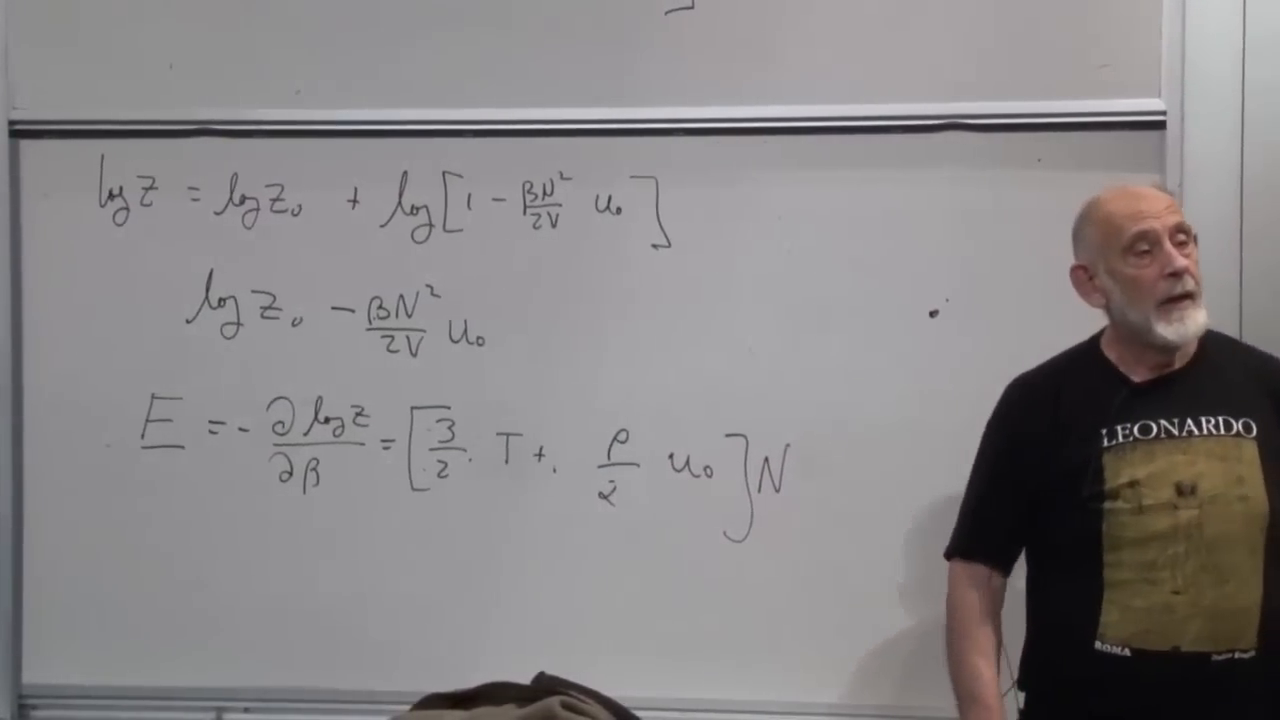
\includegraphics[width=0.90\textwidth]{lecture_06_figure_08.png}
\caption{最初の相互作用補正を示量的な
エネルギー\(N[3T/2+\rho U_0/2]\)として再編成したもの。}
\lectureframe{01:03:25}
\end{figure}

圧力の方が測定しやすい。前章の結果を用いると、
\begin{equation}
 P=T\left(\frac{\partial\log Z}{\partial V}\right)_{T,N},
 \label{eq:sm6-pressure-from-z}
\end{equation}
次を得る。
\begin{align}
 P
 &=
 \frac{NT}{V}
 +T\frac{\partial}{\partial V}
 \left(-\beta\frac{N(N-1)}{2V}U_0\right)
 +O(U^2) \notag\\
 &=
 \rho T+\frac{1}{2}\rho^2U_0
 +O\!\left(\frac{\rho U_0}{N},U^2\right).
 \label{eq:sm6-pressure-correction}
\end{align}

\begin{figure}[t]
\centering
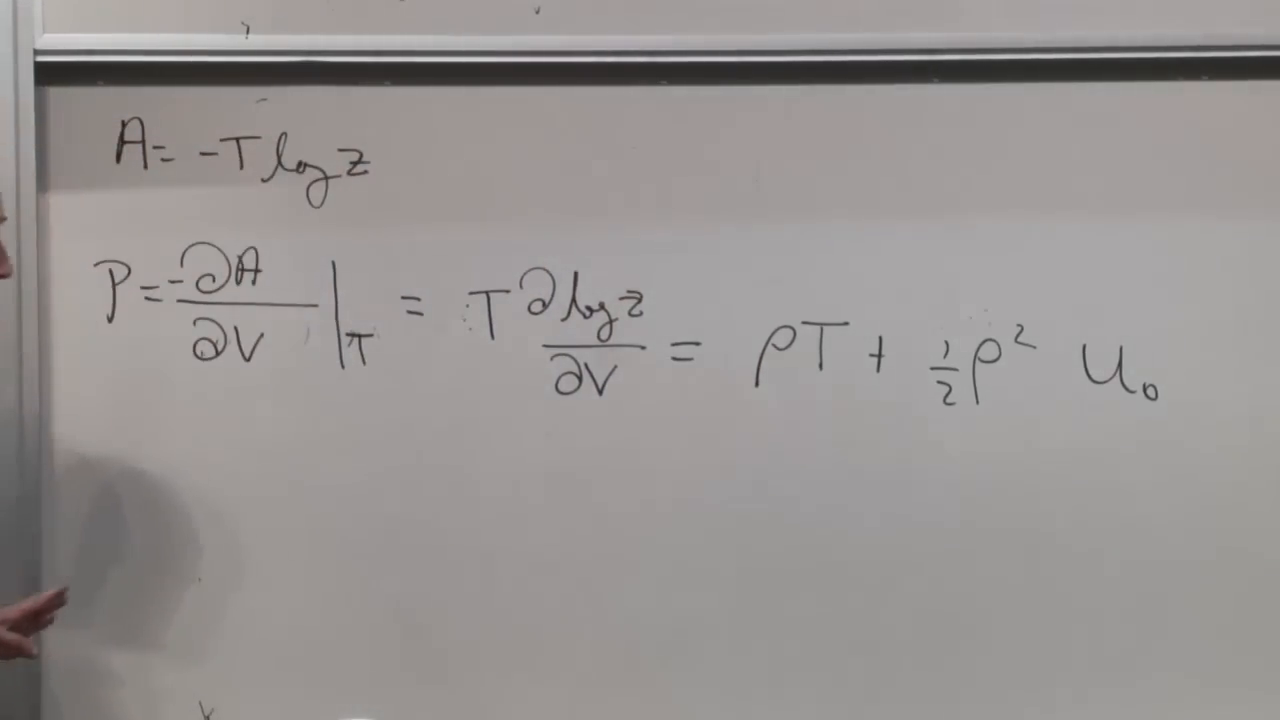
\includegraphics[width=0.90\textwidth]{lecture_06_figure_09.png}
\caption{Helmholtzの導関数から得られる圧力。最初の
密度の二次補正を含む。}
\lectureframe{01:09:50}
\end{figure}

\begin{classroomqa}
\audiencequestion{なぜ\(\rho^2\)が、別の冪ではなく、自然な
最初の補正なのか。}
\lecturerresponse{理想項は一つの粒子が
小さな領域に存在することを要し、したがって\(\rho\)のようにスケールする。相互作用は二つの
粒子が一つの分子的近傍を占めることを要し、その確率は
\(\rho^2\)のようにスケールする。因子\(1/2\)は、\((i,j)\)と\((j,i)\)が別々に数えられるのを防ぐのと同じ対の数え上げ因子である。
\lecturetimestamp{01:24:27--01:26:00}}
\end{classroomqa}

固定された温度で\(V\)を変化させ、\(\rho=N/V\)を測定し、
圧力をプロットすることができる。理想法則は線形項である。\(P(\rho)\)の曲率が
最初の相互作用補正を明らかにする。この弱ポテンシャル
近似の範囲内では、補正は明示的な温度依存性をもたない。なぜなら\eqref{eq:sm6-pressure-from-z}における因子\(T\)が
\(\beta=1/T\)を打ち消すからである。

\begin{classroomqa}
\audiencequestion{三体効果を含めなければならなくなるまで、密度はどれだけ大きくなりうるか。}
\lecturerresponse{密度の数え上げによれば、次のビリアル項は
\(\rho^3\)に比例するが、その係数は\(U_0\)だけから
推論することはできない。それは対相互作用の相関した積から、また存在するなら真の三体力から寄与を受ける。次のクラスター係数を計算し、それを\(\rho^2\)の項と比較しなければならない。推測された式を結果に昇格させるべきではない。
\lecturetimestamp{01:10:50--01:13:38}}
\end{classroomqa}

補正の大きさが小さいとき、理想気体の項が支配する。
\begin{equation}
 \begin{aligned}
 \frac{1}{2}\rho^2|U_0|&\ll \rho T,\\
 |\rho U_0|&\ll T
 \qquad\text{(parametrically)}.
 \end{aligned}
 \label{eq:sm6-ideal-validity}
\end{equation}
第二の不等式の両辺はエネルギーである。量
\(\rho U_0\)は粒子あたりの相互作用エネルギーのスケールであり、\(T\)は
運動エネルギーのスケールである。通常の希薄な室温の気体はこの領域のずっと内側にある。大きなずれが生じるのは、分子的近傍が相互作用が熱運動と競合するほど頻繁に占められるときだけである。

\begin{classroomqa}
\audiencequestion{この部屋の空気について基準を見積もることはできるか。}
\lecturerresponse{\(U_0\)を分子間相互作用エネルギーと分子体積の積として見積もり、数密度を掛け、その結果を
\(k_BT\)と比較する。粗い分子的数値は、通常の室内空気では相互作用のスケールが
はるかに小さいことを示す。分子が互いの相互作用範囲に頻繁に押し込まれるには、かなりの圧縮が必要である。
\lecturetimestamp{01:16:24--01:18:54}}
\end{classroomqa}

\begin{classroomqa}
\audiencequestion{\(U_0\)はどちらの符号もとりうるか。}
\lecturerresponse{はい。正の積分された相互作用はこの近似では正味の反発であり、圧力を\(\rho T\)より
上げる。負のそれは正味の引力であり、圧力を下げる。この符号の検査は\eqref{eq:sm6-pressure-correction}に対する即座の物理的
チェックである。
\lecturetimestamp{01:18:56--01:20:29}}
\end{classroomqa}

\begin{figure}[t]
\centering
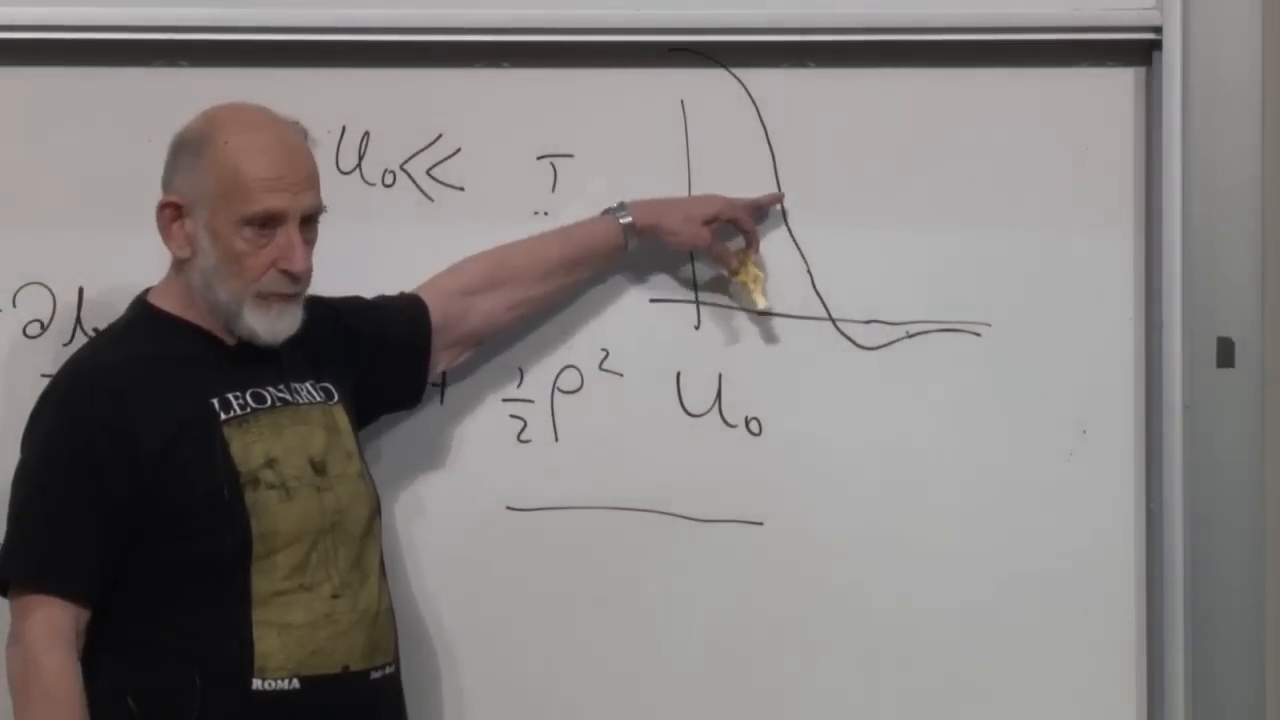
\includegraphics[width=0.90\textwidth]{lecture_06_figure_10.png}
\caption{定性的な反発および引力の対ポテンシャルプロファイルと、その補正が\(U_0\)の符号に従う圧力の式。}
\lectureframe{01:21:30}
\end{figure}

\begin{classroomqa}
\audiencequestion{静電的反発、重力引力、あるいは実際の分子間力をこの計算に組み込むことはできるか。}
\lecturerresponse{微視的ポテンシャルは原子物理学、分子物理学、あるいは量子物理学から入力される。中性分子は一般に、急峻な短距離の反発芯と、より長距離に及ぶ引力のファンデルワールス的裾を持ち、しばしば12--6ポテンシャルで模式的に表される。このような硬い芯に対しては、完全なメイヤー関数の公式を用いるべきである。重力は異なる。それは長距離的であり、その空間積分は要求される仕方では収束せず、ここで用いている通常の短距離熱力学的極限は破綻する。
\lecturetimestamp{01:20:40--01:23:03}}
\end{classroomqa}

この計算は有用な分業を例示している。微視的物理学が\(u(r)\)を与える。統計力学がそのエネルギーを\(Z\)に変え、\(Z\)の導関数がバルクの観測量を生み出し、物理的推論がその符号、密度スケーリング、示量性、妥当性の領域を検証する。形式的な操作が機械的であるのは、正しいエネルギーと近似が選ばれた後だけである。

\section{完全微分と経路依存性}

ここで数学的言語を変える。\emph{完全微分}という語句において、完全とは数値的に精密であることを意味しない。それは、1形式が真のスカラー関数の微分であることを意味する。

\(f(x,y)\)を風景の中の一点の上の高度とする。小さな変位はそれを次だけ変化させる。
\begin{equation}
 df=
 \frac{\partial f}{\partial x}\,dx+
 \frac{\partial f}{\partial y}\,dy
 =f_x\,dx+f_y\,dy.
 \label{eq:sm6-total-differential}
\end{equation}
代わりに、単に次が与えられたとしよう。
\begin{equation}
 \omega=F_x(x,y)\,dx+F_y(x,y)\,dy.
 \label{eq:sm6-one-form}
\end{equation}
\(\omega=df\)となるようなスカラー\(f\)は存在するか。混合偏導関数の等しさは次を要求する。
\begin{equation}
 \frac{\partial F_y}{\partial x}
 =
 \frac{\partial F_x}{\partial y}.
 \label{eq:sm6-exactness-condition}
\end{equation}
単連結領域上では、このゼロ回転条件は十分でもある。成分\((F_x,F_y)\)はそのとき\(f\)の勾配をなす。

\begin{figure}[t]
\centering
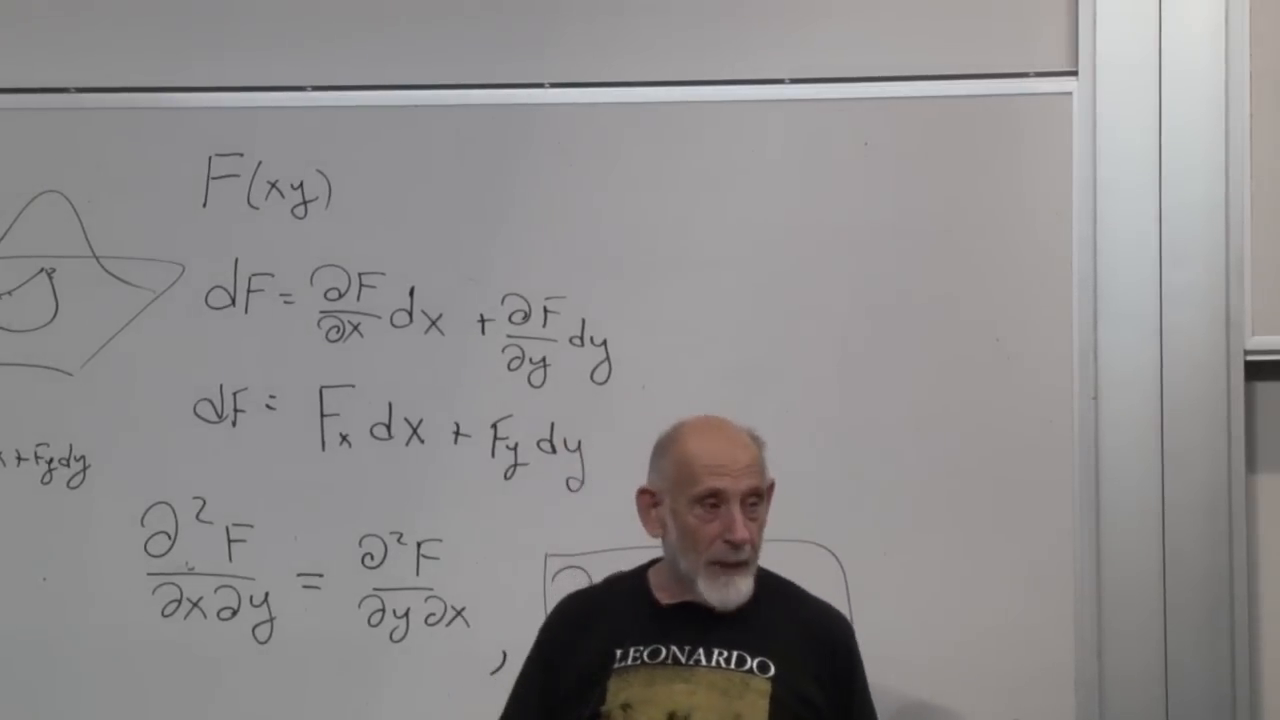
\includegraphics[width=0.90\textwidth]{lecture_06_figure_11.png}
\caption{スカラー関数としての高度、その微分、および完全性のための混合偏導関数条件。}
\lectureframe{01:34:30}
\end{figure}

同じ条件には積分的な意味がある。もし\(\omega=df\)ならば、
\begin{equation}
 \int_{\gamma:1\to2}\omega=f(2)-f(1)
 \label{eq:sm6-path-independent-integral}
\end{equation}
は端点のみに依存し、経路\(\gamma\)には依存しない。特に、
\begin{equation}
 \oint_\gamma\omega=0
 \label{eq:sm6-closed-loop-zero}
\end{equation}
がすべての可縮な閉ループに対して成り立つ。

高度はこの性質を持つ。同じ二点間を、平らな道で運転しても丘を越えて運転しても、高度の正味の変化は同じである。燃料消費はそうではない。起伏のある経路と平らな経路は一般に異なる量を消費し、閉じた旅は燃やした燃料を元に戻さない。残っている燃料の量は、拡大された状態記述においては確かに明確に定義された量であるが、それは車の位置\((x,y)\)だけの関数ではない。それは経路の記憶を伴っている。疲労も同種の類推を与える。坂を下ることは、それを登った疲労を一般には打ち消さない。

\begin{classroomqa}
\audiencequestion{完全性は保存力と同じ考えであり、曲率と関係しているのか。}
\lecturerresponse{回転がゼロの力場は局所的に保存的であり、ポテンシャルを許すので、言葉遣いは密接に関係している。平行移動と曲率もまた、閉ループの変化を局所的な幾何学的情報に結びつけるが、それはより広い主題である。ここでは初等的な主張のみが必要である。ゼロ回転は局所的な経路独立性を意味し、領域について通常の大域的條件が課される。
\lecturetimestamp{01:39:22--01:41:07}}
\end{classroomqa}

二つの例がこの判定を具体的にする。まず次を取る。
\begin{equation}
 F_x=y,\qquad F_y=x.
 \label{eq:sm6-exact-example}
\end{equation}
両方の交差導関数は\(1\)に等しく、確かに
\begin{equation}
 \omega=y\,dx+x\,dy=d(xy).
 \label{eq:sm6-exact-example-potential}
\end{equation}
次に一つの符号を変える。
\begin{equation}
 F_x=y,\qquad F_y=-x.
 \label{eq:sm6-inexact-example}
\end{equation}
すると
\begin{equation}
 \frac{\partial F_x}{\partial y}=1,
 \qquad
 \frac{\partial F_y}{\partial x}=-1,
 \label{eq:sm6-inexact-cross-derivatives}
\end{equation}
となるので、これらの二つの成分を勾配として持つスカラー\(f(x,y)\)は存在しない。

\begin{figure}[t]
\centering
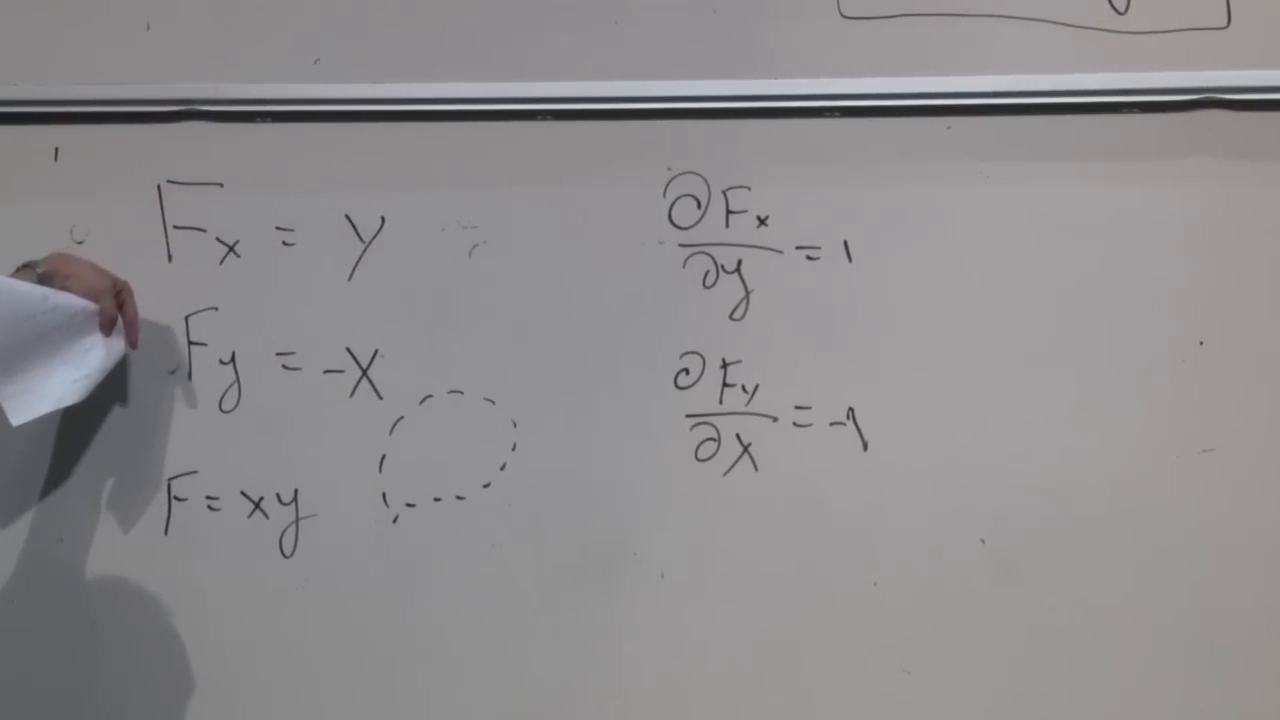
\includegraphics[width=0.90\textwidth]{lecture_06_figure_12.png}
\caption{\(f=xy\)によって生成される完全な例と、交差導関数が\(1\)および\(-1\)である不完全な例。}
\lectureframe{01:44:50}
\end{figure}

\section{熱と仕事は状態関数ではない}

粒子数が固定された単純な圧縮性系では、二つの独立な平衡変数が状態を決定する。\((T,V)\)、\((E,V)\)、あるいは、基本関係にとって特に自然な\((S,V)\)を用いてもよい。したがって
\begin{equation}
 E=E(S,V),
 \end{equation}
であり、その完全微分は
\begin{equation}
 dE=
 \left(\frac{\partial E}{\partial S}\right)_V dS+
 \left(\frac{\partial E}{\partial V}\right)_S dV
 =T\,dS-P\,dV.
 \label{eq:sm6-fundamental-relation}
\end{equation}
である。

\begin{classroomqa}
\audiencequestion{断熱とは、遅いこと、断熱されたこと、可逆であること、それともエントロピー一定であることを意味するのか。}
\lecturerresponse{この用語は文脈によって異なる使われ方をする。ここで考える平衡経路では、変化は準静的かつ熱的に断熱されており、したがって可逆かつ等エントロピーである。単に断熱された不可逆過程は依然としてエントロピーを生成しうる一方、量子断熱定理はパラメータのゆっくりした変化を強調する。
\lecturetimestamp{01:47:13--01:47:54}}
\end{classroomqa}

エントロピーを固定したとき、膨張は気体のエネルギーを
\(-P\,dV\) だけ変化させる。体積を固定したとき、可逆的な熱の移動はそれを
\(T\,dS\) だけ変化させる。したがって、次のように書くのが有用である。
\begin{equation}
 \begin{aligned}
 \delta W_{\mathrm{on}}&=-P\,dV,
 &\delta Q_{\mathrm{rev}}&=T\,dS,\\
 dE&=\delta Q_{\mathrm{rev}}+\delta W_{\mathrm{on}}.&&
 \end{aligned}
 \label{eq:sm6-first-law-increments}
\end{equation}
記号 \(\delta\) は、\(d\) ではなく、熱と仕事が状態関数の微分ではなく経路の増分であることを先取りしている。

\begin{figure}[t]
\centering
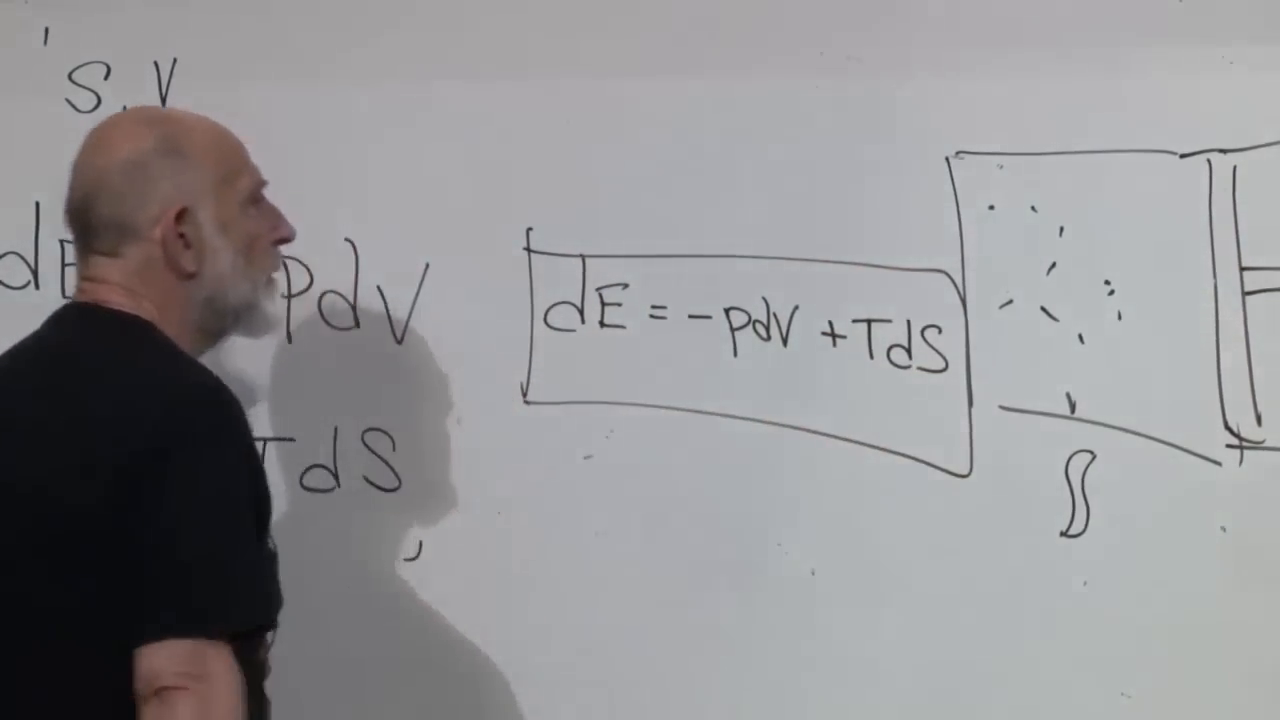
\includegraphics[width=0.90\textwidth]{lecture_06_figure_13.png}
\caption{ピストン系に対する第一法則：
\(dE=-P\,dV+T\,dS\)。}
\lectureframe{01:50:28}
\end{figure}

\begin{classroomqa}
\audiencequestion{\(-P\,dV\) は気体に対してなされる仕事を表すのか、それとも気体がなす仕事を表すのか。}
\lecturerresponse{
\eqref{eq:sm6-first-law-increments} の規約では、気体に対してなされる仕事である。膨張の間 \(dV>0\)、気体はピストンに対して正の仕事をするので、気体に対してなされる仕事は負であり、気体はエネルギーを失う。二つの記述は大きさが等しく符号が反対である。
\lecturetimestamp{01:51:23--01:52:27}}
\end{classroomqa}

等式 \(\delta Q_{\mathrm{rev}}=T\,dS\) を、そのまま任意の不可逆加熱に拡張してはならない。一般には、
\begin{equation}
 dS=\frac{\delta Q}{T_{\mathrm{boundary}}}+dS_{\mathrm{prod}},
 \qquad dS_{\mathrm{prod}}\ge 0.
 \label{eq:sm6-entropy-production}
\end{equation}
以下に述べる完全微分の議論は準静的平衡経路に関するものであり、その場合には可逆関係が適切である。

\begin{classroomqa}
\audiencequestion{状態空間の議論におけるすべての経路は、平衡状態を通ると仮定されているのか。}
\lecturerresponse{はい。操作は十分にゆっくり行われるので、\(P\)、\(T\)、\(E\)、\(S\)、\(V\) は経路に沿って well-defined のままである。熱と仕事の経路依存性は、系が平衡から遠く離れて駆動されることを必要としない。
\lecturetimestamp{01:54:30--01:54:39}}
\end{classroomqa}

熱が完全微分であるかどうかを調べるには、\((E,V)\) を座標として用い、第一法則を整理する。
\begin{equation}
 \delta Q_{\mathrm{rev}}=dE+P(E,V)\,dV.
 \label{eq:sm6-heat-one-form}
\end{equation}
もし \(dQ=\delta Q_{\mathrm{rev}}\) となる状態関数 \(Q(E,V)\) が存在するならば、その偏導関数は
\begin{equation}
 \left(\frac{\partial Q}{\partial E}\right)_V=1,
 \qquad
 \left(\frac{\partial Q}{\partial V}\right)_E=P.
 \label{eq:sm6-hypothetical-heat-derivatives}
\end{equation}
でなければならない。そのとき混合導関数の等しさは
\begin{equation}
 \begin{aligned}
 \frac{\partial}{\partial V}
 \left(\frac{\partial Q}{\partial E}\right)_V
 &=\frac{\partial}{\partial E}
 \left(\frac{\partial Q}{\partial V}\right)_E,\\
 0&=\left(\frac{\partial P}{\partial E}\right)_V.
 \end{aligned}
 \label{eq:sm6-heat-exactness-requirement}
\end{equation}
を要求する。

\begin{classroomqa}
\audiencequestion{これは \(F_x\,dx+F_y\,dy\) に用いられるのとまさに同じ回転テストか。}
\lecturerresponse{はい。\(dE\) と \(dV\) の係数は \(1\) と
\(P(E,V)\) である。それらの交差導関数は \(0\) と
\((\partial P/\partial E)_V\) である。熱が完全微分であるのは、それらの導関数が一致する場合に限られる。
\lecturetimestamp{01:54:39--01:54:52}}
\end{classroomqa}

\begin{figure}[t]
\centering
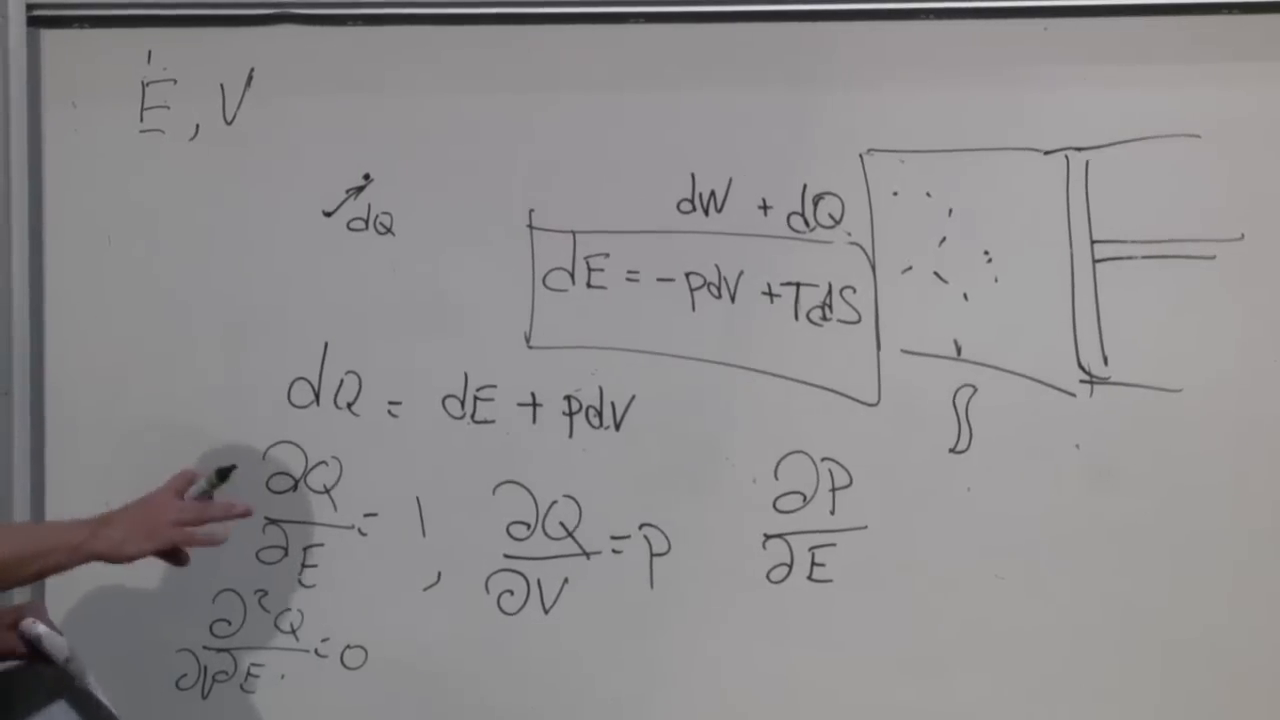
\includegraphics[width=0.90\textwidth]{lecture_06_figure_14.png}
\caption{熱の一次形式 \(dE+P\,dV\) と、それが状態関数の微分である場合に要求される混合導関数。}
\lectureframe{01:58:10}
\end{figure}

この要求はすでに物理的にありそうにない。体積を固定して気体にエネルギーを加えると、一般にはその圧力が変化する。理想気体は直接的な計算を与える。
\begin{equation}
 PV=NT,
 \qquad
 E=\frac{3}{2}NT
 \quad\Longrightarrow\quad
 P=\frac{2E}{3V}.
 \label{eq:sm6-ideal-pressure-energy}
\end{equation}
したがって
\begin{equation}
 \left(\frac{\partial P}{\partial E}\right)_V
 =\frac{2}{3V}\ne0.
 \label{eq:sm6-heat-curl-fails}
\end{equation}
回転テストは失敗する。\(\delta Q_{\mathrm{rev}}\) は完全微分ではない。仕事の増分 \(\delta W_{\mathrm{on}}=-P\,dV\) も同じ理由で失敗する。

\begin{figure}[t]
\centering
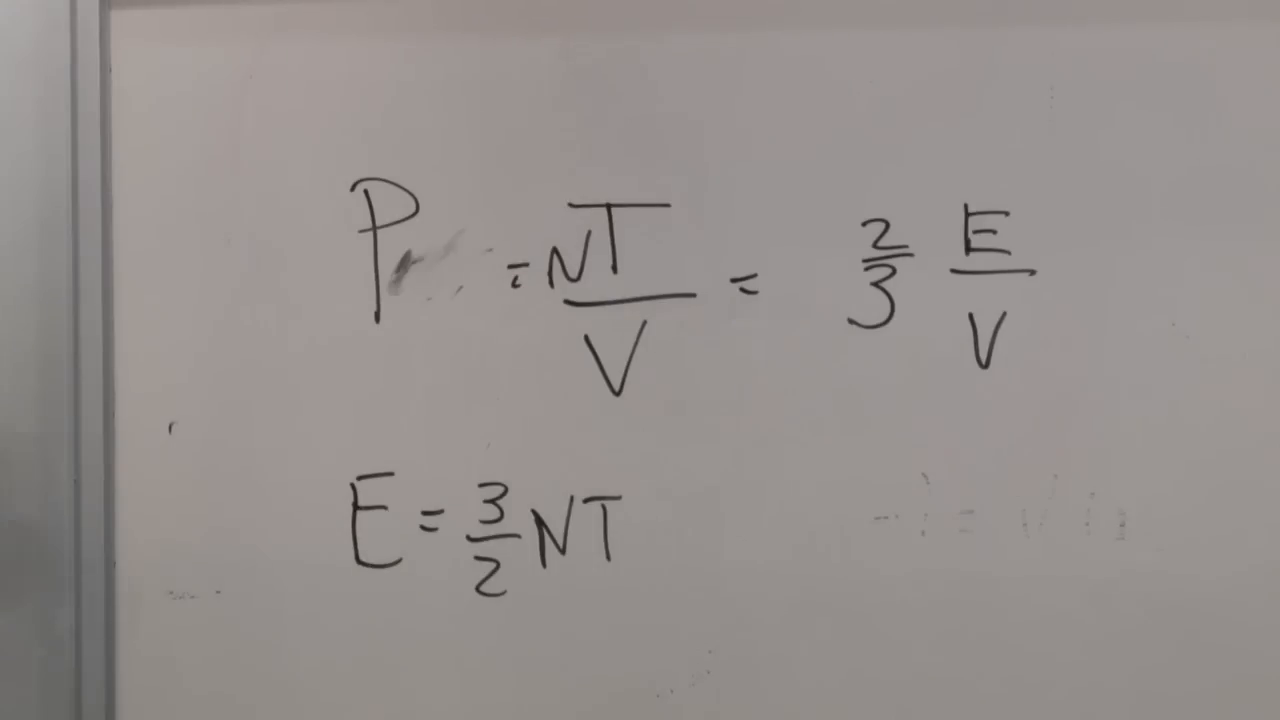
\includegraphics[width=0.90\textwidth]{lecture_06_figure_15.png}
\caption{理想気体の関係を組み合わせると
\(P=2E/(3V)\) となる。}
\lectureframe{02:00:00}
\end{figure}

\begin{figure}[H]
\centering
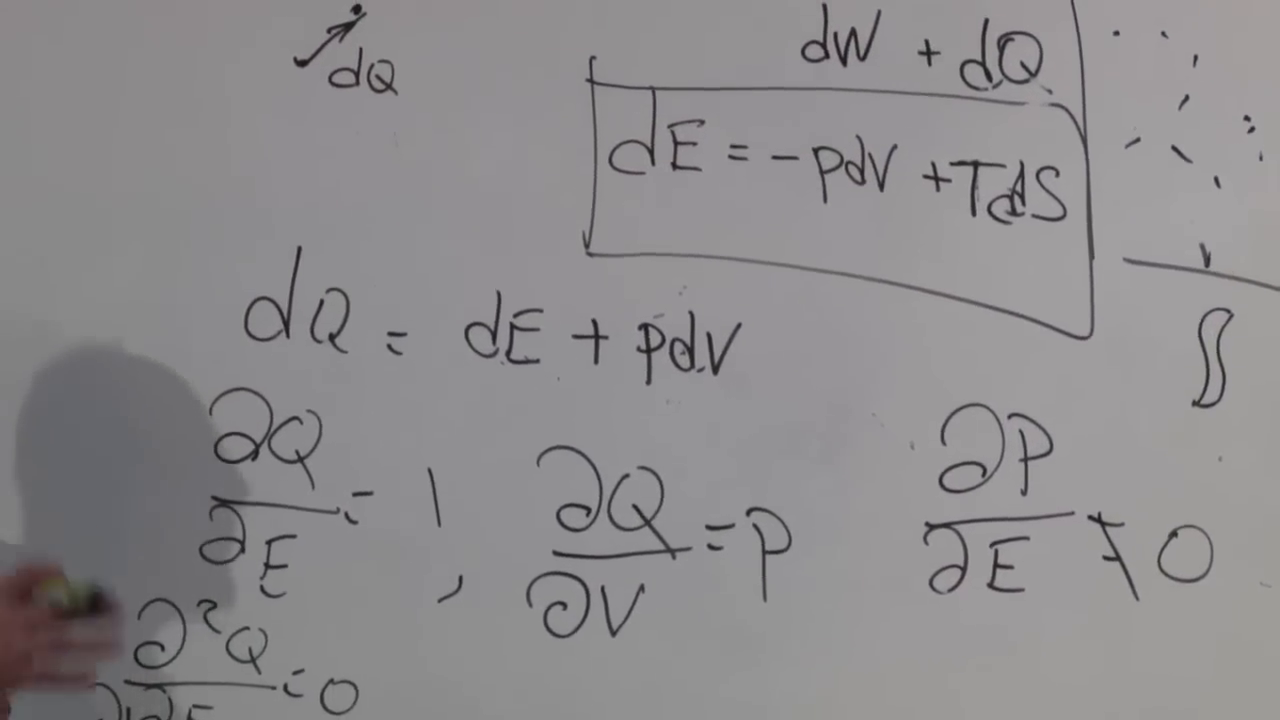
\includegraphics[width=0.90\textwidth]{lecture_06_figure_16.png}
\caption{完成した議論：\((\partial P/\partial E)_V\ne0\) であるから、熱の一次形式は完全微分でありえない。}
\lectureframe{02:00:35}
\end{figure}

閉じた平衡サイクルに対して、
\begin{equation}
 \oint dE=0,
 \qquad
 \oint\delta Q_{\mathrm{rev}}
 =-\oint\delta W_{\mathrm{on}}.
 \label{eq:sm6-cycle-balance}
\end{equation}
系は同じエネルギーに戻るが、熱と仕事は別々に消える必要はない。それらの値は状態空間を通る経路に依存する。これが、作動物質が初期の熱力学的状態に戻るにもかかわらず、サイクル機関が熱を吸収して正味の仕事を供給できる理由である。

\begin{classroomqa}
\audiencequestion{この経路依存性は、機関効率、ヒステリシス、記憶と関係しているのか。}
\lecturerresponse{機関サイクルはそれを直接利用する。閉サイクルの熱入力は、状態関数 \(E\) が初期値に戻る間、正味の仕事出力と釣り合う。ヒステリシスと記憶も経路依存性を含むが、それらはしばしば追加の内部変数や非平衡物理を必要とする。現在の結論はより狭く、すでに可逆平衡経路に対して成り立つ。熱と仕事は移動であり、熱力学的状態に蓄えられた性質ではない。
\lecturetimestamp{02:02:21--02:03:17}}
\end{classroomqa}

議論の二つの半分がここで出会う。測定は、その制御と平衡条件が指定されて初めて意味を持つ。近似は、その小さなパラメータと失敗基準が指定されて初めて意味を持つ。熱力学量は、その微分が経路非依存性のテストに合格して初めて状態関数である。いずれの場合も、規律ある数学は物理的解釈を置き換えるのではなく、その解釈がどこで正当化されるかを正確に教えてくれる。
\chapter{音、量子振動子、そして第二法則}

\lectureoverview{第二法則が目的地であるが、その道を準備する二つの具体的な計算がある。音速は、熱力学的な導関数がどのようにして観測可能な運動になるかを試すものである。次に調和振動子は、剛い自由度に対する古典的な等分配の破綻を明らかにし、量子力学がモードを一つずつ励起する仕組みを示す。最後に、可逆な微視的力学と増大するエントロピーの間の見かけの矛盾に戻り、位相空間の流れ、粗視化、カオス、再帰を用いて、第二法則を例外のない力学的禁止ではなく、圧倒的に確からしい法則として述べる。}

\section{第二法則に関する約束}

中心的な問題は述べるのは容易だが、説明するのは難しい。ニュートンの方程式は可逆である。ある微視的な履歴が許されるなら、時間反転した履歴もまた許される。それにもかかわらず第二法則は、巨視的な過程には好ましい向きがあり、それは通常増大するエントロピーによって特徴づけられると述べている。我々はその緊張に至るであろうが、すぐではない。まず統計力学が具体的な情報を生み出すのを見て、その後、初等的な計算の中で、古典物理学が量子物理学に道を譲らざるを得なかった歴史的な難問に出会う方がよい。

第一の例は数値的で意図的に粗い。希薄気体中の音速を見積もる。第二の例はその仮定の範囲内で厳密である。熱浴中の調和振動子の平均エネルギーを計算する。振動子は等分配から量子化されたエネルギー準位へ、一つのモードから無限に多くのモードへ、そして最後に多粒子系がその初期状態を忘れるとはどういうことかという問いに戻ることになる。

\section{音速の分子的スケール}

希薄気体中の小さな過密度を想像せよ。分子が混み合った領域を離れるためにそれは広がるので、その伝播速度は分子速度と同程度であるはずである。等分配は一分子の運動エネルギーを与える。\begin{equation}
 \frac{3}{2}k_B T
 =\frac{1}{2}m\expect{v^2},
 \qquad
 \expect{v^2}=\frac{3k_B T}{m}.
 \label{eq:sm7-molecular-speed}
\end{equation}
ここで温度は絶対零度から測られ、実験室単位を望むので\(k_B\)が復元されている。この議論はスケールの見積もりにすぎない。分子の二乗平均平方根速度それ自体は集団的な音波の速度ではない。

より系統的な導出では、気体の小さな要素を考える。反対側の面にかかる圧力が等しくないため正味の力が生じ、その加速度は質量密度に反比例する。結果は次の形をとる。\begin{equation}
 c_s^2=
 \left(\frac{\partial P}{\partial \rho_m}\right)_{\cal C},
 \qquad
 \rho_m=m\rho,
 \label{eq:sm7-sound-general}
\end{equation}
ここで\(\rho\)は数密度であり、添字\({\cal C}\)は擾乱によって従われる熱力学的条件を指定する。板書の計算では次を用いる。\begin{equation}
 P=\rho k_B T
 \quad\Longrightarrow\quad
 \frac{1}{m}
 \left(\frac{\partial P}{\partial\rho}\right)_T
 =\frac{k_B T}{m}.
 \label{eq:sm7-sound-isothermal}
\end{equation}
これは等温音速の見積もりである。これは\eqref{eq:sm7-molecular-speed}とは、速度の二乗で\(3\)の因子、あるいは速度で\(\sqrt{3}\)だけ異なる。

\begin{figure}[t]
\centering
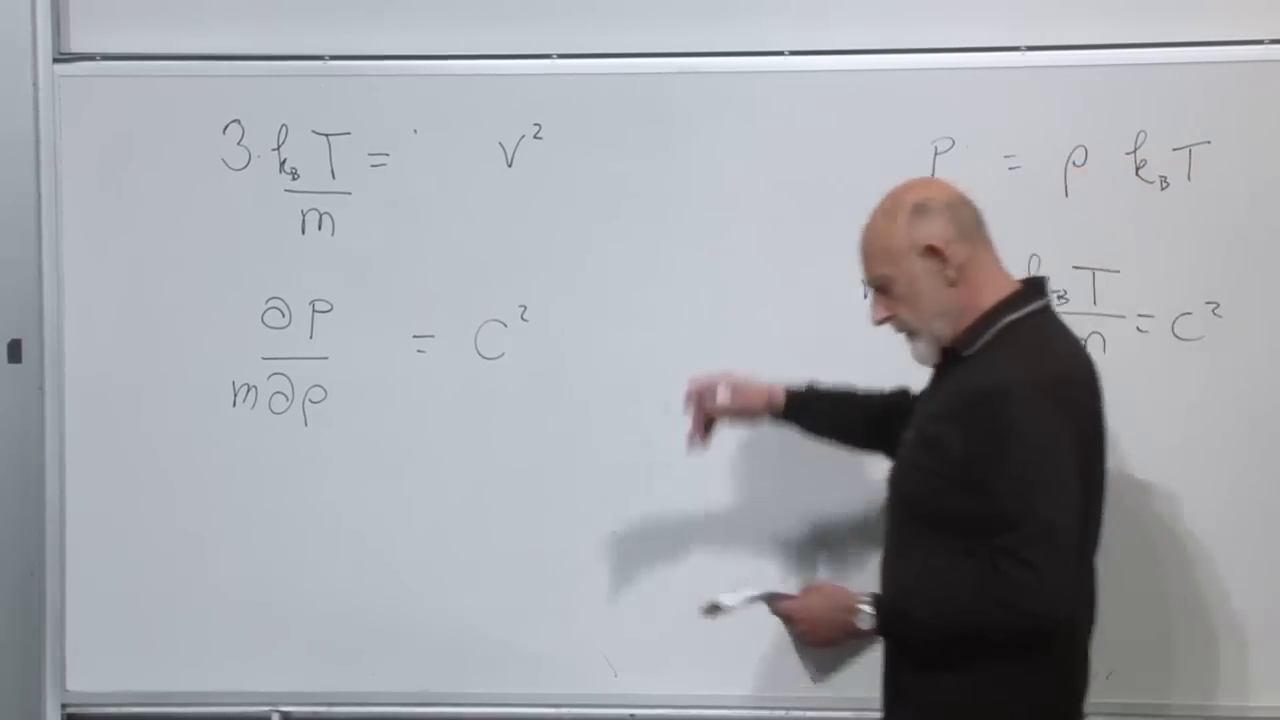
\includegraphics[width=0.90\textwidth]{lecture_07_figure_02.png}
\caption{分子速度の見積もり、圧力の導関数、そして理想気体の代入を一緒に示したもの。}
\lectureframe{00:08:55}
\end{figure}

重要な改良がある。小振幅の音波は通常、隣接する要素間で熱が流れるよりも速く気体を圧縮・膨張させる。したがって局所的な運動は近似的に断熱的であり、等温的ではない。\begin{equation}
 c_s^2=
 \left(\frac{\partial P}{\partial\rho_m}\right)_S.
 \label{eq:sm7-sound-adiabatic}
\end{equation}
断熱指数\(\gamma\)をもつ理想気体では、\begin{equation}
 P\rho_m^{-\gamma}=\text{constant},
 \qquad
 c_s^2=\gamma\frac{P}{\rho_m}
       =\gamma\frac{k_B T}{m}.
 \label{eq:sm7-sound-ideal-adiabatic}
\end{equation}
室温の二原子空気では\(\gamma\simeq 7/5\)である。したがって固定温度の計算は有用な第一の見積もりであり、断熱的な導関数が物理的に適切な改良を与える。

粗い値を用いると\begin{equation}
\begin{aligned}
 k_B&\simeq1.3\times10^{-23}\ {\rm J\,K^{-1}},
 &T&\simeq300\ {\rm K},\\
 m_{\rm air}&\simeq4\times10^{-26}\ {\rm kg}.&&
\end{aligned}
 \label{eq:sm7-air-data}
\end{equation}
分子の見積もりはおよそ\(500\ {\rm m\,s^{-1}}\)である。ここでの温度はケルビン単位の絶対温度でなければならず、華氏のようなオフセット尺度ではない。よく知られた音速は\(300\ {\rm m\,s^{-1}}\)の程度であり、断熱理想気体の式は室温でおよそ\(340\ {\rm m\,s^{-1}}\)を与える。したがって粗い計算は正しい物理的スケールを見出したことになる。

\begin{figure}[t]
\centering
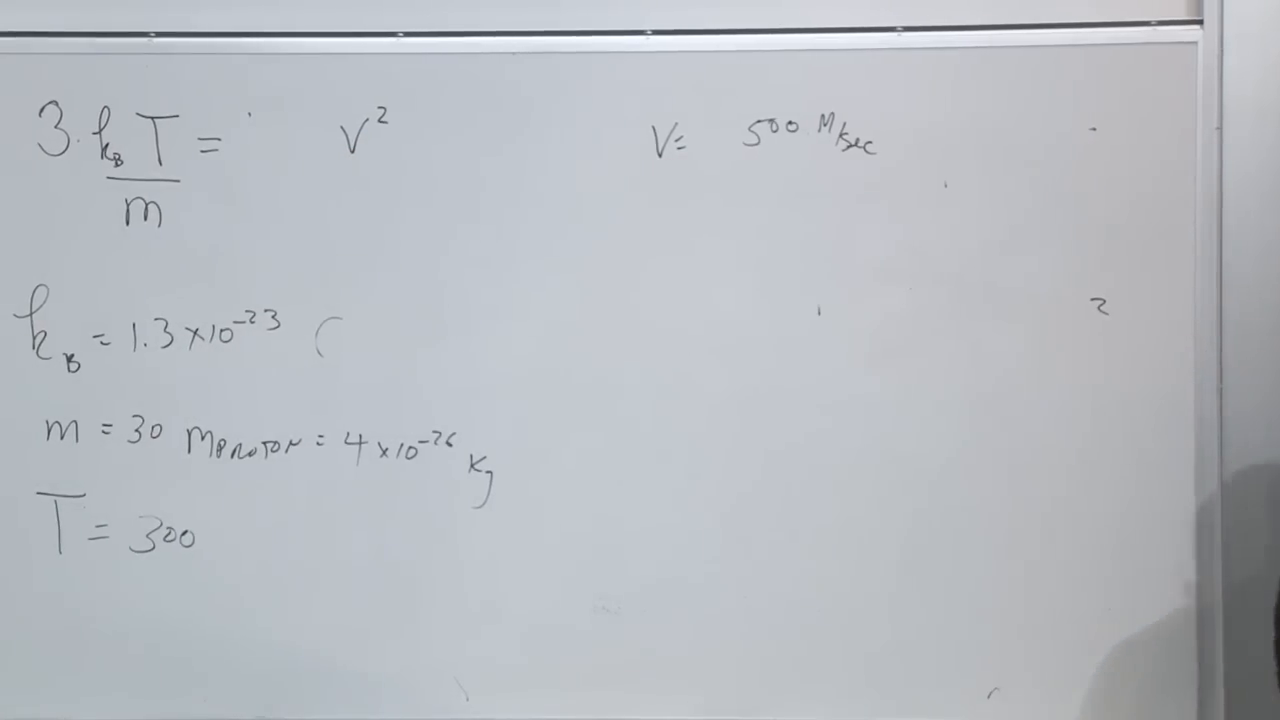
\includegraphics[width=0.90\textwidth]{lecture_07_figure_03.png}
\caption{ボルツマン定数、およそ\(30\)陽子質量に近い有効分子質量、そして\(T\simeq300\ {\rm K}\)を用いた室温空気の見積もり。}
\lectureframe{00:10:55}
\end{figure}

微視的な説明が得られるずっと以前から、密度の関数としての圧力の測定から音速を決定することができた。統計的な議論は、その結果得られる巨視的な速度が個々の分子の熱速度によって定まるという際立った解釈を付け加える。

\begin{classroomqa}
\audiencequestion{中性子は分子質量に加えるべきなのか、また窒素についての数\(14\)は陽子だけを数えているのか。}
\lecturerresponse{引用された原子量はすでに陽子と中性子を数えている。分子状窒素は原子量およそ\(14\)の原子を2個含むので、その質量はおよそ\(28\)陽子質量である。この見積もりには\(28\)を\(30\)に丸めるだけで十分である。
\lecturetimestamp{00:10:58--00:11:16}}
\end{classroomqa}

\begin{classroomqa}
\audiencequestion{因子\(3\)は3つの並進方向から来たが、音は1つの方向に伝播する。それなら\(3\)の因子は除くべきではないか。}
\lecturerresponse{それは、3次元の二乗平均平方根分子速度を1次元の伝播速度と同一視してはならないことを正しく警告している。冒頭の議論は桁程度の描像にすぎなかった。制御された答えは、圧力の導関数と、波に適した熱力学的条件から得られる。
\lecturetimestamp{00:11:12--00:12:00}}
\end{classroomqa}

\begin{classroomqa}
\audiencequestion{その導関数は、波の間、温度が一定に保たれると仮定したのか。}
\lecturerresponse{示された理想気体の代入はそうした。温度を固定することは、ごく小さな擾乱に対するもっともらしい暫定的見積もりである。標準的な精密化は、通常の音が近似的に断熱的であるというものであり、それにより等温導関数が\(\left(\partial P/\partial\rho_m\right)_S\)に置き換わる。
\lecturetimestamp{00:12:59--00:14:01}}
\end{classroomqa}

\begin{classroomqa}
\audiencequestion{圧力と密度の変動がどちらも小さいなら、それらの導関数も小さくなるのか。}
\lecturerresponse{いいえ。導関数は、無限小極限における2つの小さな変動の比である。\(\delta P\)と\(\delta\rho\)はどちらも小さくあり得るが、\(\delta P/\delta\rho\)は有限のままであり、波の速度を定める。
\lecturetimestamp{00:14:03--00:14:23}}
\end{classroomqa}

\begin{classroomqa}
\audiencequestion{気体が圧縮されると、気体から液体や固体へ移る場合のように、音速は上昇すべきなのか。}
\lecturerresponse{はい。導関数は考察中の状態で評価され、\(P(\rho,T)\)は線形のままでいる必要はない。分子が互いに近くに押し込まれると、状態方程式は非理想的になり、\(\partial P/\partial\rho\)はかなり大きくなり得る。
\lecturetimestamp{00:14:25--00:15:13}}
\end{classroomqa}

\begin{classroomqa}
\audiencequestion{値\(500\ {\rm m\,s^{-1}}\)はあらゆる圧力で使えるのか。}
\lecturerresponse{いいえ。それは理想気体方程式が有用な近似となる低密度領域に属する。密度のより高い冪が\(P(\rho,T)\)に入ると、導関数、したがって音速は圧力と密度に依存する。
\lecturetimestamp{00:15:14--00:16:29}}
\end{classroomqa}

\begin{classroomqa}
\audiencequestion{音がほぼ分子速度で広がるという元の描像も、密度が増すにつれて破綻するのか。}
\lecturerresponse{おそらくそうである。その描像は希薄気体に合わせて仕立てられたものである。高密度では集団的相互作用がますます重要になり、まさにそのために状態方程式の導関数がより一般的な記述となるのである。
\lecturetimestamp{00:16:32--00:16:53}}
\end{classroomqa}

\begin{classroomqa}
\audiencequestion{なぜ窒素分子の質量は\(28\)ではなく、およそ\(30\)陽子質量と書かれたのか。}
\lecturerresponse{見積もりに適した数値精度だけが必要なので、\(28\)は\(30\)に丸められた。元の\(500\ {\rm m\,s^{-1}}\)という見積もりを\(\sqrt{3}\simeq1.7\)で割っても\(300\ {\rm m\,s^{-1}}\)に近くなるが、補正を計算する制御された方法は断熱導関数である。
\lecturetimestamp{00:16:54--00:17:27}}
\end{classroomqa}

\section{熱浴中の1つの古典的振動子}

ここで、自由に並進する分子を1つの調和振動子に置き換え、その他すべてを熱浴として扱う。ばねについた質量が直接の描像であるが、この模型ははるかに広い。電磁空洞モードは振動し、結晶中の原子は振動し、平衡からわずかにずらされたほとんど任意の安定な系は、主要な次数で調和運動を行う。

平衡からの変位\(x\)、運動量\(p\)、質量\(m\)、ばね定数\(\kappa\)を用いると、ハミルトニアンは
\begin{equation}
 H(x,p)=\frac{p^2}{2m}+\frac{\kappa x^2}{2},
 \qquad
 \omega=\sqrt{\frac{\kappa}{m}}.
 \label{eq:sm7-classical-hamiltonian}
\end{equation}
である。熱浴は\(T\)を固定し、この時点から再び\(k_B=1\)を用いるので、\(\beta=1/T\)となる。室温と平衡にある振動子は\(300\ {\rm K}\)付近の温度をもち、液体ヘリウムに浸されたものはわずか数ケルビンの温度しかもたない。太陽の中心に置かれたと仮定したばねはばねとして生き残らないであろうが、この例は環境の役割を明瞭にする。ボルツマン重みは因子分解する:
\begin{equation}
 e^{-\beta H}
 =e^{-\beta p^2/(2m)}
  e^{-\beta\kappa x^2/2}.
 \label{eq:sm7-factorized-weight}
\end{equation}

\begin{figure}[t]
\centering
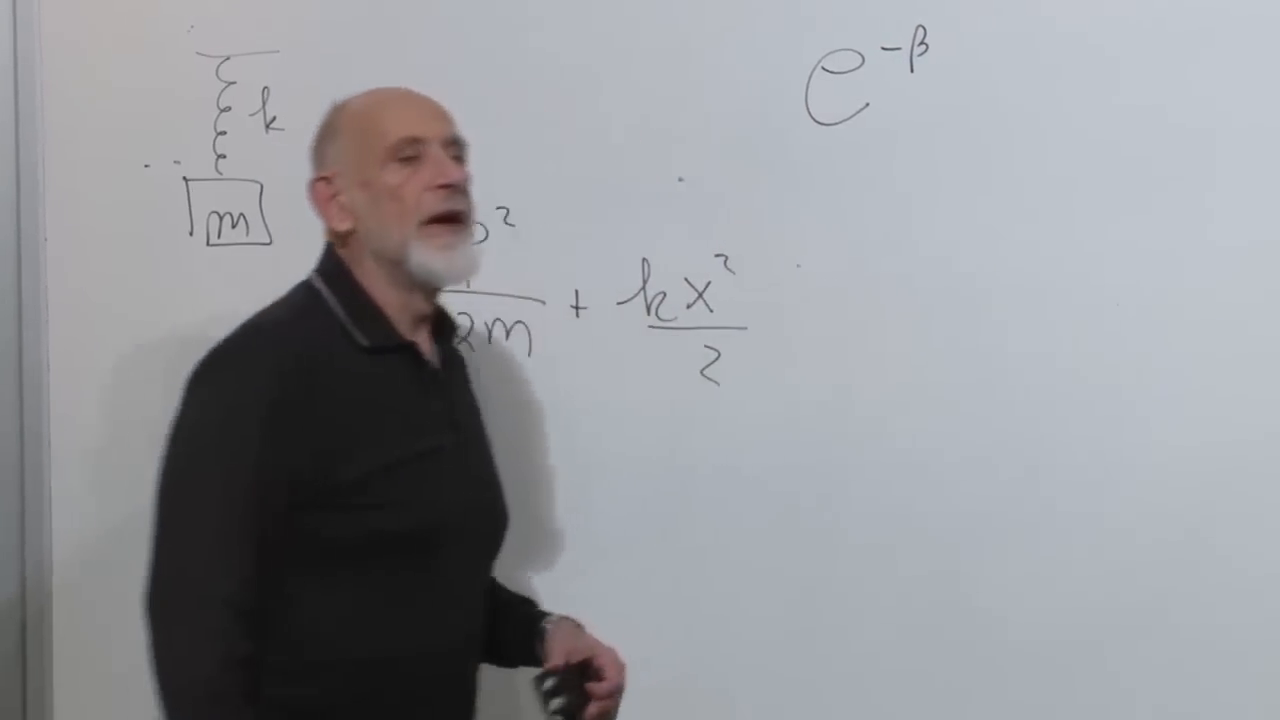
\includegraphics[width=0.90\textwidth]{lecture_07_figure_04.png}
\caption{ばね-質量振動子とその運動エネルギーおよびポテンシャルエネルギーのハミルトニアン。}
\lectureframe{00:20:55}
\end{figure}

自由気体とは異なり、位置積分は単に容器の体積を与えるだけではない。復元ポテンシャルが各変位に重みを付ける：
\begin{equation}
 Z_{\rm cl}
 =\frac{1}{h}\int_{-\infty}^{\infty}dp
             \int_{-\infty}^{\infty}dx\,
 e^{-\beta p^2/(2m)}
 e^{-\beta\kappa x^2/2}.
 \label{eq:sm7-classical-z}
\end{equation}
因子\(1/h\)は一次元古典分配関数を無次元にする。これは\(\beta\)に依存せず平均エネルギーに影響し得ないため、板書の計算では省略されている。

\begin{figure}[t]
\centering
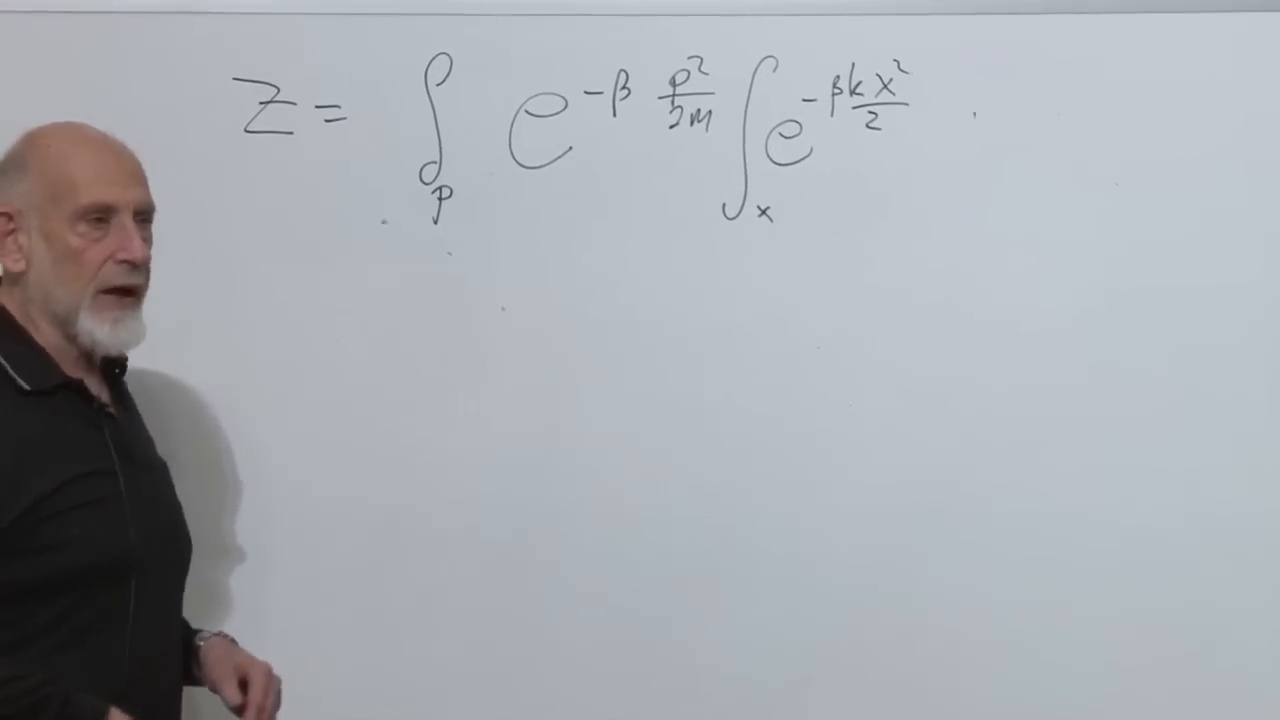
\includegraphics[width=0.90\textwidth]{lecture_07_figure_05.png}
\caption{運動量と変位のガウス積分に分離された古典振動子の分配関数。}
\lectureframe{00:22:55}
\end{figure}

運動量積分に対しては
\begin{equation}
 q=\sqrt{\frac{\beta}{2m}}\,p,
 \qquad
 dp=\sqrt{\frac{2m}{\beta}}\,dq.
 \label{eq:sm7-p-gaussian-substitution}
\end{equation}
と置く。位置積分に対しては
\begin{equation}
 y=\sqrt{\frac{\beta\kappa}{2}}\,x,
 \qquad
 dx=\sqrt{\frac{2}{\beta\kappa}}\,dy.
 \label{eq:sm7-x-gaussian-substitution}
\end{equation}
と置く。\(\int_{-\infty}^{\infty}e^{-u^2}\,du=\sqrt{\pi}\)であるから、板書で用いられる規格化されていない位相空間積分は
\begin{equation}
 \int dp\,dx\,e^{-\beta H}
 =\frac{2\pi}{\beta}\sqrt{\frac{m}{\kappa}}
 =\frac{2\pi}{\beta\omega}.
 \label{eq:sm7-classical-z-unnormalized}
\end{equation}
となる。位相空間のセルを復元すると、
\begin{equation}
 Z_{\rm cl}=\frac{2\pi}{h\beta\omega}
           =\frac{1}{\beta\hbar\omega}.
 \label{eq:sm7-classical-z-normalized}
\end{equation}

エネルギーに対しては\(\beta\)依存性のみが重要である：
\begin{equation}
 \begin{aligned}
 \log Z_{\rm cl}&=\text{constant}-\log\beta,\\
 \expect{H}
 &=-\frac{\partial\log Z_{\rm cl}}{\partial\beta}\\
 &=\frac{1}{\beta}=T.
 \end{aligned}
 \label{eq:sm7-classical-energy}
\end{equation}

\begin{figure}[t]
\centering
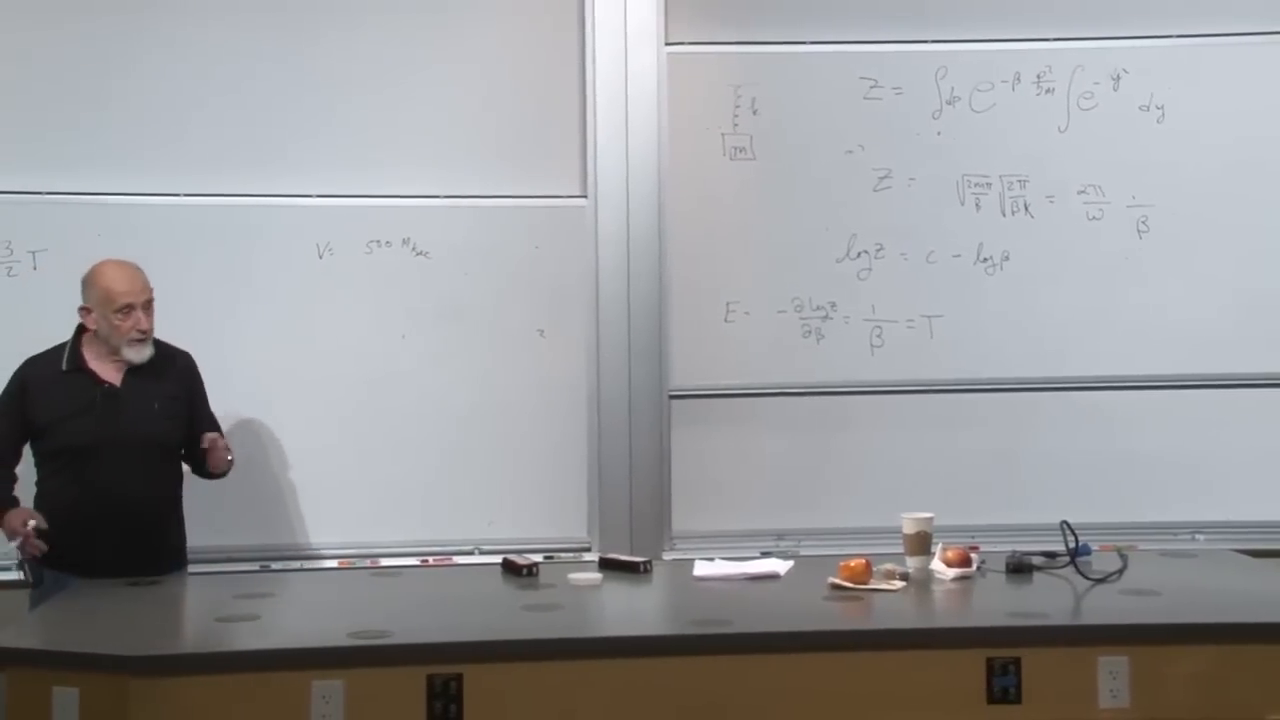
\includegraphics[width=0.90\textwidth]{lecture_07_figure_06.png}
\caption{右の板書における完全な古典的連鎖：ガウス分解、\(Z\propto(\beta\omega)^{-1}\)、そして\(\expect{H}=1/\beta=T\)。}
\lectureframe{00:30:15}
\end{figure}

これは一つの空間的振動子であるから、\(3\)の因子は存在しない。また二つの独立な二次項があるため、\(1/2\)の残りの因子も存在しない。各ガウス積分は\(T/2\)に寄与する：
\begin{equation}
 \expect{K}=\frac{T}{2},
 \qquad
 \expect{U}=\frac{T}{2},
 \qquad
 \expect{H}=T.
 \label{eq:sm7-equipartition-oscillator}
\end{equation}
これが最も有用な形でのエネルギー等分配則である：古典ハミルトニアンにおける各独立な二次項は\(T/2\)に寄与する。

答えは\(m\)と\(\kappa\)の両方に依存しない。運動自体はこれらのパラメータに依存する：
\begin{equation}
 \expect{p^2}=mT,
 \qquad
 \expect{x^2}=\frac{T}{\kappa},
 \qquad
 \expect{\dot{x}^2}=\frac{T}{m}.
 \label{eq:sm7-classical-fluctuations}
\end{equation}
したがって、より重い質量はよりゆっくりと運動し、より硬いばねはより小さな振幅を持つが、平均エネルギーは依然として\(T\)である。\(\kappa\)が途方もなく大きくなると、このことは厄介になる。動かないほど硬いばねは凍結した拘束のように見えるべきであるのに、古典的なエネルギー等分配は依然としてそれにエネルギー\(T\)を割り当てる。

\begin{classroomqa}
\audiencequestion{\(\kappa\to\infty\)のとき、分配関数はゼロに近づく。それでもその対数はどのようにして用いることができるのか？}
\lecturerresponse{\(\kappa\)を有限だが任意に大きく保つ。\(\log Z\)への寄与は加法的であり\(\beta\)に依存しないため、\(\beta\)による微分は依然として\(T\)を与える。極限における不快感は現実のものである：古典的計算は内部的に整合しているが、非常に硬い振動子に必要な自然の特徴を欠いている。
\lecturetimestamp{00:34:01--00:34:54}}
\end{classroomqa}

\begin{classroomqa}
\audiencequestion{理想気体の分配関数には\(N!\)が必要であった。ここにも同様の階乗があるべきだろうか？}
\lecturerresponse{いいえ。我々は一つの指定された振動子を研究しているのであり、\(N\)個の同一粒子を並べ替えているのではない。多くの独立なラベル付きモードに対しては、分配関数は掛け合わされる。不可弁別因子は別の数え上げ問題に属する。
\lecturetimestamp{00:35:03--00:35:40}}
\end{classroomqa}

\section{なぜ古典的エネルギー等分配は危機であったか}

実在の分子は構造のない点ではない。二原子分子は振動し得る結合を含み、したがって内部振動子を持つ。素朴な古典的勘定では、通常の温度においてさえそのモードに追加の熱エネルギーを割り当てることになる。意図的に図式的な勘定では、一つの振動子を活性化すると\(3T/2\)のエネルギーが\(5T/2\)に向かって上昇する。精密な熱容量の記帳は回転自由度も含み、エネルギーとその温度微分を区別しなければならない。決定的な実験的事実はより単純である：硬い内部モードは、古典的エネルギー等分配が要求するようには低温で寄与しなかった。

分子が内部構造を持つことを否定するか、それは不合理であるが、あるいは古典力学に何かが欠けていることを認めるかである。欠けているものは量子力学である。我々が必要とするのはそのほんのわずかである：調和振動子が等間隔のエネルギー準位を持つということだけである。

\section{量子振動子}

まずエネルギーの原点をずらし、励起スペクトルを
\begin{equation}
 E_n^{\rm exc}=n\hbar\omega,
 \qquad n=0,1,2,\ldots.
 \label{eq:sm7-shifted-spectrum}
\end{equation}
と書く。分配関数は今や位相空間積分ではなく真の和である：
\begin{align}
 Z_{\rm exc}
 &=\sum_{n=0}^{\infty}e^{-\beta n\hbar\omega} \notag\\
 &=1+x+x^2+\cdots
  =\frac{1}{1-x},
 \qquad x=e^{-\beta\hbar\omega}, \notag\\
 &=\frac{1}{1-e^{-\beta\hbar\omega}}.
 \label{eq:sm7-quantum-z}
\end{align}

\begin{figure}[t]
\centering
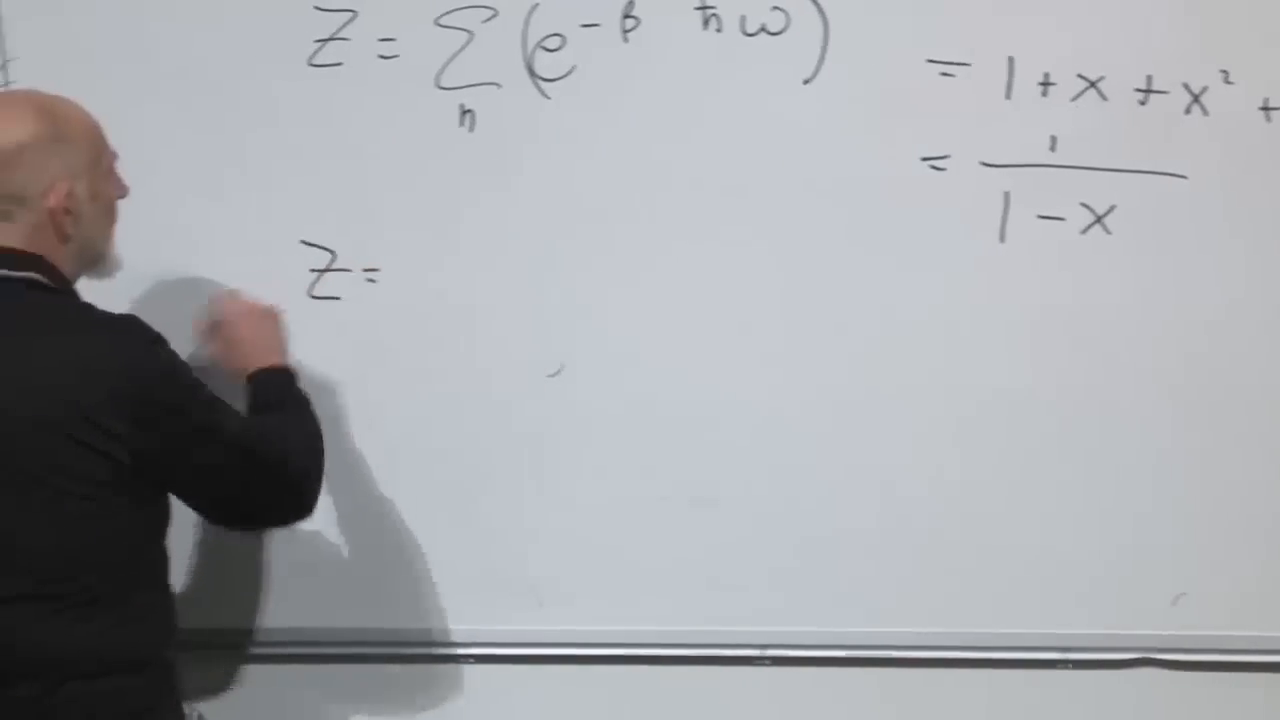
\includegraphics[width=0.90\textwidth]{lecture_07_figure_07.png}
\caption{等間隔準位と量子振動子分配関数の幾何級数による評価。}
\lectureframe{00:42:05}
\end{figure}

微分すると平均励起エネルギーが得られる：
\begin{align}
 E_{\rm exc}
 &=-\frac{\partial\log Z_{\rm exc}}{\partial\beta}
  =-\frac{1}{Z_{\rm exc}}
    \frac{\partial Z_{\rm exc}}{\partial\beta}
 \notag\\
 &=\hbar\omega\,
   \frac{e^{-\beta\hbar\omega}}
        {1-e^{-\beta\hbar\omega}}
  =\frac{\hbar\omega}{e^{\beta\hbar\omega}-1}.
 \label{eq:sm7-quantum-energy}
\end{align}

\begin{figure}[t]
\centering
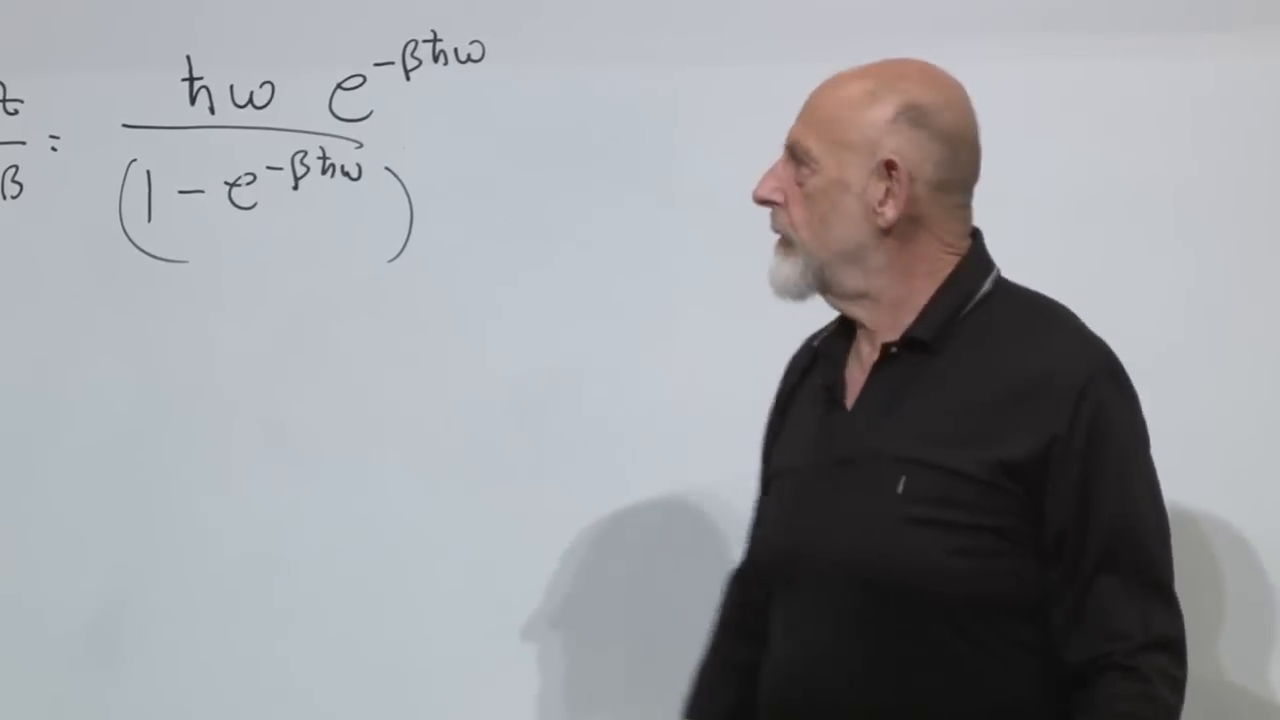
\includegraphics[width=0.90\textwidth]{lecture_07_figure_08.png}
\caption{量子分配関数の\(\beta\)微分から得られる熱励起エネルギー。}
\lectureframe{00:46:05}
\end{figure}

\subsection{高温}

\(\beta\hbar\omega\ll1\)のとき、
\begin{equation}
 e^{-\beta\hbar\omega}
 =1-\beta\hbar\omega
  +O\!\left((\beta\hbar\omega)^2\right).
 \label{eq:sm7-high-t-expansion}
\end{equation}
\eqref{eq:sm7-quantum-energy}の分子は\(\hbar\omega\)に近づき、分母は主要項で\(\beta\hbar\omega\)である。したがって
\begin{equation}
 E_{\rm exc}\simeq\frac{1}{\beta}=T.
 \label{eq:sm7-high-t-energy}
\end{equation}
量子論的答えは、多くの準位間隔が熱エネルギーの中に収まるとき、古典的エネルギー等分配を回復する。

\subsection{低温}

\(\beta\hbar\omega\gg1\) のとき、指数関数は極めて小さい：
\begin{equation}
 E_{\rm exc}
 \simeq\hbar\omega e^{-\beta\hbar\omega}.
 \label{eq:sm7-low-t-energy}
\end{equation}
振動子の熱励起は指数関数的に抑制される。ずらした表記ではほとんどゼロである；物理的な零点エネルギーは以下で復元される。

\begin{figure}[t]
\centering
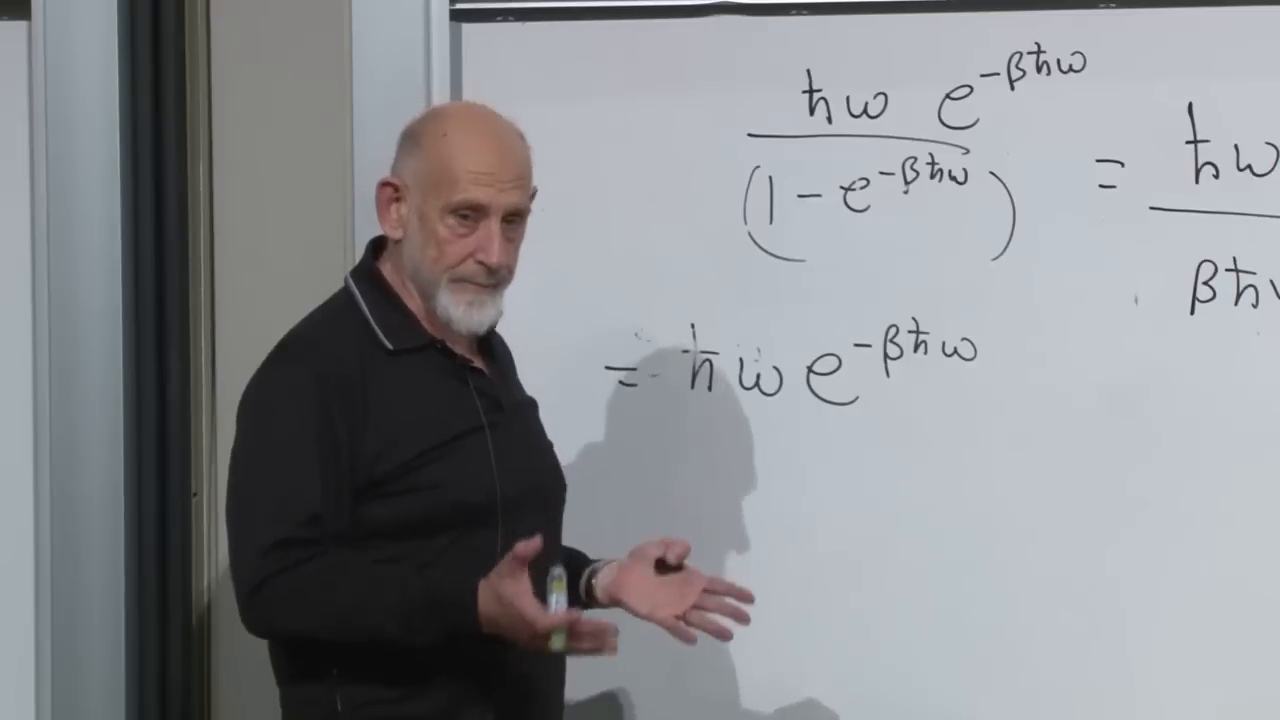
\includegraphics[width=0.90\textwidth]{lecture_07_figure_09.png}
\caption{低温展開：最初の熱励起は \(e^{-\beta\hbar\omega}\) によって抑制される。}
\lectureframe{00:51:55}
\end{figure}

クロスオーバーは次が成り立つときに起こる：
\begin{equation}
 \beta\hbar\omega\sim1,
 \qquad\text{or equivalently}\qquad
 T\sim\hbar\omega.
 \label{eq:sm7-crossover}
\end{equation}
この条件には直接的な意味がある。古典的な等分配則では振動子のエネルギーは \(T\) となる。そのスケールが1つの準位間隔を下回ると、量子効果は避けられなくなる。したがって
\begin{equation}
\begin{aligned}
 \hbar\omega\gg T&:\quad \text{frozen and quantum},\\
 \hbar\omega\ll T&:\quad \text{active and classical}.
\end{aligned}
 \label{eq:sm7-regimes}
\end{equation}
より硬いばねはより大きな \(\omega=\sqrt{\kappa/m}\) をもつので、古典的に振る舞うにはより高い温度を必要とする。

\section{物質を加熱すると自由度が現れる}

低温では、二原子分子はその硬い結合振動が凍結しているため、熱的に点粒子のように振る舞うことができる。\(T\) が \(\hbar\omega\) を超えて上昇すると、振動モードが活性化する。回転モードはより低いスケールで活性化するかもしれない；さらに高い温度ではより多くの内部運動が現れ、最終的には原子が電離する。加熱は単に固定されたモードのリストにより多くのエネルギーを注ぎ込むだけではない。それは低温では見えなかった自由度を明らかにする。

想像上の入れ子分子がこの点を鮮明にする。2つの原子は硬いばねで結ばれているが、見かけ上の1つの原子はそれ自体、さらに硬いばねで結ばれた対である。低い \(T\) では、両方の構造は点的に見える。最初のしきい値で外側の振動が現れる；2番目のしきい値で内側の構造が現れる。系の複雑さは、一度に1つのエネルギー・スケールずつ明らかになる。

\begin{classroomqa}
\audiencequestion{振動子がすでに古典的領域にあるとき、さらに加熱するとばねが硬くなったり振動数が変化したりするのか？}
\lecturerresponse{いいえ。ばね定数と振動数は固定されたままである。より高い温度はより大きな典型的運動量と振幅を生み、したがってより大きなエネルギーを生む。硬さは古典的法則が始まる温度を決めるのであって、温度に依存してばねが硬くなるのではない。
\lecturetimestamp{01:03:17--01:05:11}}
\end{classroomqa}

\subsection{結晶とアインシュタインの比熱}

結晶は非常に多くの振動モードを含む。古典的な等分配則はすべての活性な振動子に \(T\) スケールのエネルギーを割り当てるため、低温での熱容量を過大評価する。アインシュタインの 1907 模型は結晶振動を量子力学的に扱い、熱エネルギーがそれらの準位間隔に達するまでなぜ抑制されるかを示した。より正確な固体模型はモード振動数の分布を許すが、凍結の原理はすでにアインシュタインの計算に存在している。

\begin{classroomqa}
\audiencequestion{これはアインシュタインがノーベル賞を受賞した仕事であり、量子力学が確立された後に初めて現れたのか？}
\lecturerresponse{いいえ。ノーベル賞の授賞理由は光電効果に関するものであった。比熱模型は 1907 に発表され、量子力学の完全な基礎が理解されるずっと前であった。アインシュタインは、後に成熟した理論の側面に反対したにもかかわらず、決定的な量子のアイデアを受け入れ、発展させた。
\lecturetimestamp{00:58:38--01:03:16}}
\end{classroomqa}

\begin{classroomqa}
\audiencequestion{古典統計力学は、離散状態の和を位置と運動量にわたる一見一様な積分に置き換えた。何がその状態の数え方を正当化するのか？}
\lecturerresponse{究極的な正当化は量子力学から来る。高温極限では、
\[
 Z_{\rm exc}\simeq\frac{1}{\beta\hbar\omega},
\]
これは無次元の古典的結果
\eqref{eq:sm7-classical-z-normalized} と正確に一致する。準位間隔が分解されないとき、位相空間の量子セルは古典的位相空間測度になる。
\lecturetimestamp{00:59:38--01:03:06}}
\end{classroomqa}

\subsection{弦は無限に多くの振動子を含む}

バイオリンやギターの弦は基準モードに分解される：基本振動、より高い倍音、そして次第に短くなる波長である。数学的には無限に多くの振動子モードが存在する。もし古典的な等分配則がそのすべてにエネルギー \(T\) を割り当てるなら、熱平衡にある弦は無限のエネルギーをもつことになる。量子力学がその破局を防ぐ。最短波長のモードは最も高い振動数をもち、任意の有限温度で凍結したままである；\(T\) が上昇するにつれて次第により多くのモードが活性化する。同じ論理は後に黒体放射の基礎となる。

\begin{figure}[t]
\centering
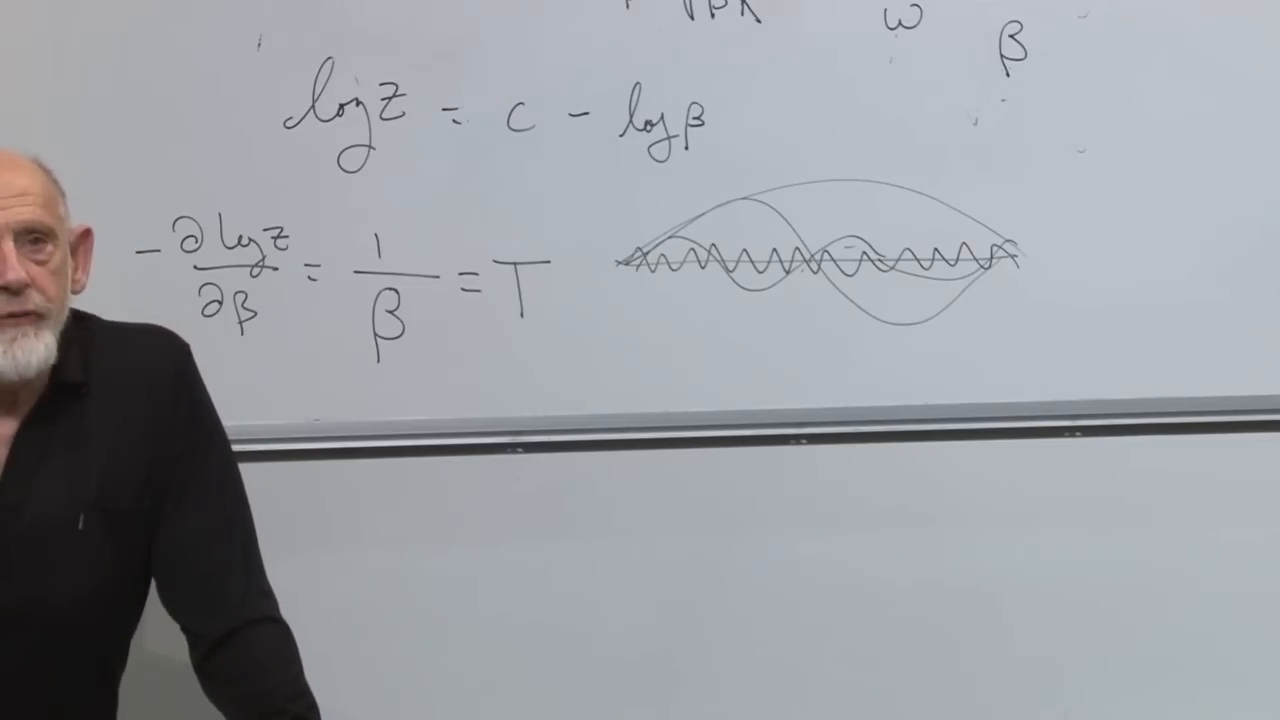
\includegraphics[width=0.90\textwidth]{lecture_07_figure_10.png}
\caption{弦上に重ね合わされたいくつかの基準モード。連続的な弦がなぜ無限の調和振動子の集まりであるかを示している。}
\lectureframe{01:09:30}
\end{figure}

\begin{classroomqa}
\audiencequestion{量子から古典へのクロスオーバーは直接観測できるのか、また加熱によって低温での振る舞いを逆転させることができるのか。}
\lecturerresponse{はい。結晶の比熱の温度依存性によって、振動モードの凍結とそれに続く活性化は明瞭に測定可能となる。
\lecturetimestamp{01:09:11--01:10:13}}
\end{classroomqa}

\begin{classroomqa}
\audiencequestion{多数の振動子に対して、単一振動子の分配関数を各モードごとに繰り返すのか。}
\lecturerresponse{独立なモードに対しては、
\[
\begin{aligned}
 Z_{\rm tot}&=\prod_j Z_j,&
 \log Z_{\rm tot}&=\sum_j\log Z_j,\\
 E_{\rm tot}&=\sum_j E_j.&&
\end{aligned}
\]
\(\hbar\omega_j\gg T\) となるモードは熱的寄与が指数関数的に小さく、しきい値より下のモードは無視できない寄与をする。
\lecturetimestamp{01:10:14--01:11:00}}
\end{classroomqa}

\begin{classroomqa}
\audiencequestion{振動子の零点エネルギー \(\hbar\omega/2\) はどうなったのか。}
\lecturerresponse{物理的な準位は
\[
 E_n=\left(n+\frac12\right)\hbar\omega.
\]
したがって
\[
 \begin{aligned}
 Z_{\rm phys}
 &=e^{-\beta\hbar\omega/2}Z_{\rm exc},\\
 E_{\rm phys}
 &=\frac{\hbar\omega}{2}
  +\frac{\hbar\omega}{e^{\beta\hbar\omega}-1}.
 \end{aligned}
\]
共通のずれは準位の確率、エントロピー、熱容量、熱励起エネルギーを変えないが、絶対平均エネルギーを \(\hbar\omega/2\) だけずらす。\(Z\) における乗因子は \(\beta\) に依存するので、絶対エネルギーを求める場合には捨ててはならない。
\lecturetimestamp{01:11:08--01:11:37}}
\end{classroomqa}

\section{可逆性のパズルとしての第二法則}

ここで、約束した問題に戻ることができる。第二法則は、通常のマクロな発展が不可逆であり、エントロピーが増大する傾向があると述べている。ミクロなハミルトニアン的発展は可逆である。可逆な厳密状態の写像が、どのようにしてマクロ状態の不可逆な法則を生み出すのだろうか。

系を高次元位相空間の一点で表す。
\[
 \Gamma=(q_1,\ldots,q_N,p_1,\ldots,p_N).
\]
我々の知識は通常、厳密な一点ではない。それが体積 \(\Omega_A\) のコンパクトなパッチ \(A\) 上の一様な確率密度であると仮定する。
\begin{equation}
 f(\Gamma)=
 \begin{cases}
  1/\Omega_A,&\Gamma\in A,\\
  0,&\Gamma\notin A.
 \end{cases}
 \label{eq:sm7-uniform-blob}
\end{equation}
\(k_B=1\) とする単位系では、その細粒ギブズエントロピーは
\begin{equation}
 S_{\rm fine}
 =-\int d\Gamma\,f\log f
 =\log\Omega_A.
 \label{eq:sm7-blob-entropy}
\end{equation}
パッチが小さいほど情報が多く、エントロピーは低い。これにより符号が定まる。不確かさが増大すると占有領域が広がり、\(\log\Omega_A\) が増大する。

\begin{figure}[t]
\centering
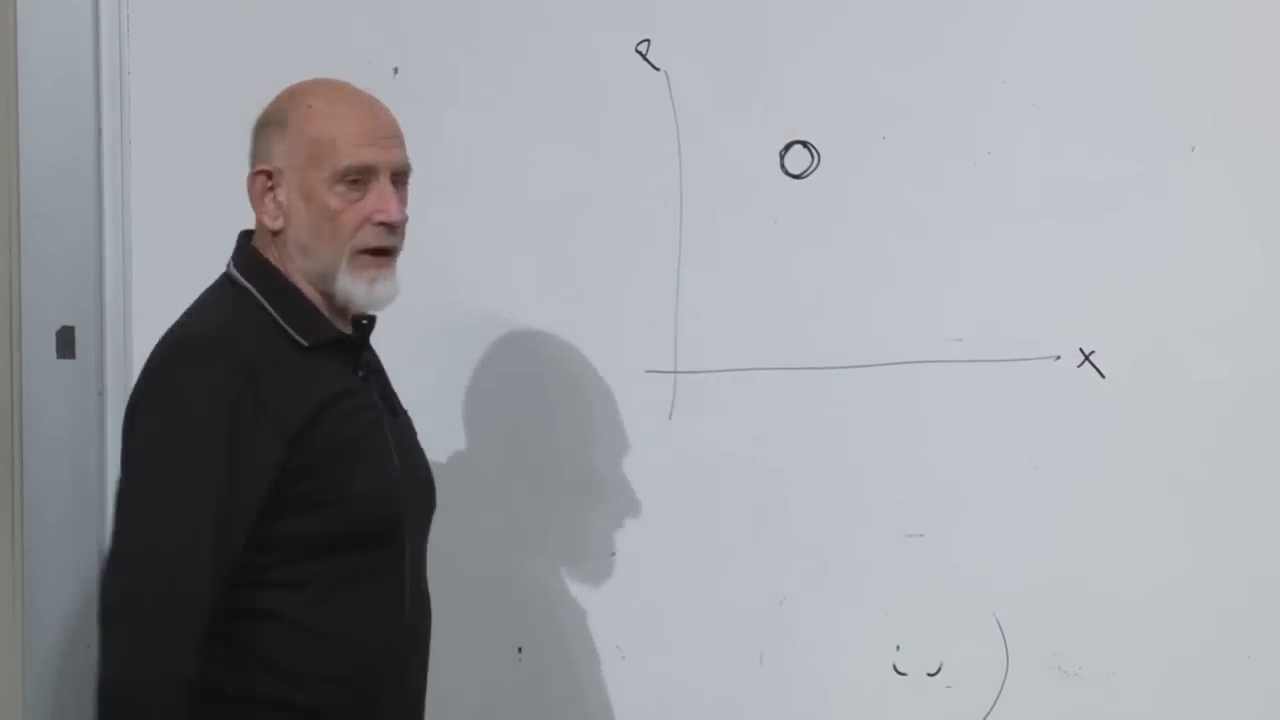
\includegraphics[width=0.90\textwidth]{lecture_07_figure_11.png}
\caption{完全な位置-運動量位相空間の模式的な二次元断面におけるコンパクトな確率パッチ。}
\lectureframe{01:20:20}
\end{figure}

\begin{classroomqa}
\audiencequestion{系は物理的に描かれたパッチの内部にとどまるよう拘束されているのか、またすでに平衡にあるのか。}
\lecturerresponse{いいえ。パッチは初期状態について知られていることを記述するものであり、位相空間における壁ではない。それは平衡分布である必要はない。部屋の隅のタンクに初め閉じ込められた気体は、特殊な非平衡情報の具体的な例である。
\lecturetimestamp{01:14:55--01:15:24}}
\end{classroomqa}

\section{リウヴィル流と粗視化された増大}

リウヴィルの定理は、ハミルトニアン流が位相空間体積を保存すると述べている。厳密なパッチは並進し、伸び、折り畳まれ、極めて薄くなりうるが、
\begin{equation}
 \Omega_{A(t)}=\Omega_{A(0)},
 \qquad
 S_{\rm fine}(t)=S_{\rm fine}(0).
 \label{eq:sm7-liouville}
\end{equation}
離散的な類似物は状態の可逆な置換である。サイコロが二つの状態のいずれかにあると初めに知っている場合、一対一の発展はそれらがどの二つの状態であるかを変えうるが、可能性の数を変えることはない。

現実の記述は有限の分解能をもつ。量子力学は自然な位相空間セルを与えるが、古典的な実験は量子論を持ち出さなくても有限の測定能力をもつ。ハミルトニアン流の下で、パッチは長く薄い蛇になりうる。隣接する折り目の間隔が分解能の尺度を下回ると、我々は分解できない各近傍を粗いセルで置き換える。厳密な占有体積は固定されたままであるが、粗いセルの合併は増大する。
\begin{equation}
 \Omega_{\rm coarse}(t)\geq\Omega_{A(t)},
 \qquad
 S_{\rm coarse}(t)=\log\Omega_{\rm coarse}(t).
 \label{eq:sm7-coarse-entropy}
\end{equation}

\begin{figure}[t]
\centering
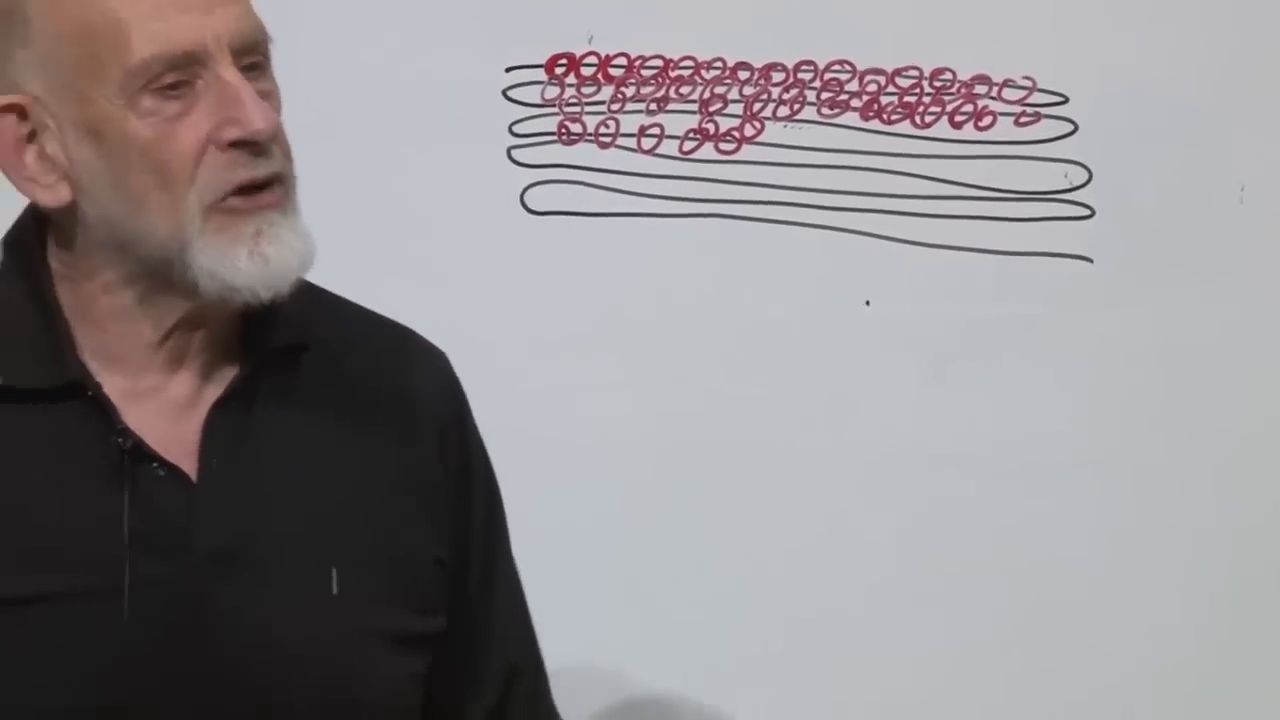
\includegraphics[width=0.90\textwidth]{lecture_07_figure_12.png}
\caption{有限分解能のセルを通して見た体積保存フィラメント。厳密な黒いフィラメントはその面積を保つが、赤い粗いセルはより大きな有効領域を占める。}
\lectureframe{01:22:10}
\end{figure}

\begin{classroomqa}
\audiencequestion{粗いセルが重なり合っている。これはリウヴィルの定理に反するのか。}
\lecturerresponse{いいえ。リウヴィルは厳密なフィラメントを支配し、それは一対一かつ体積保存のままである。重なりは我々のぼやけた記述に属する。我々は状態がどの細い糸に含まれるかという情報を捨て去ったのである。
\lecturetimestamp{01:21:32--01:21:50}}
\end{classroomqa}

有用な類推は綿である。すべての繊維の材料体積はほぼ固定されたままでありうるが、ほぐされた綿の塊は、個々の繊維を分解できない観察者にとって大きな見かけの体積を占める。同様に、位相空間のパッチはより細い触手を成長させ、それらの触手はさらに細い触手を発達させる。任意の固定された有限分解能は、最終的にそれらを追跡できなくなる。

\begin{classroomqa}
\audiencequestion{エントロピーは古典的には増大して見えるだけで、量子力学が基本的な分解能の限界を課すことによってその増大を実在のものにするのだろうか。}
\lecturerresponse{粗視化の議論は量子限界を必要としない。エントロピーは系と、その記述において保持される巨視的な区別とを合わせて指し示す。無限の微視的情報があれば、細視化エントロピーは一定である。いかなる固定された有限の分解能のもとでも、カオス的なフィラメントはやがて分解されなくなり、粗視化エントロピーは増大する。
\lecturetimestamp{01:24:04--01:25:20}}
\end{classroomqa}

\section{カオス、有限の到達可能領域、そして平衡化}

箱の中の気体では、位置は有界である。有限の全エネルギーを固定すれば、たとえすべてのエネルギーが一時的に一つの粒子に集中しても、運動量もまた有界である。したがって、通常の閉じ込めの仮定のもとで、力学的に到達可能なエネルギー殻は有限の測度をもつ。

\begin{figure}[t]
\centering
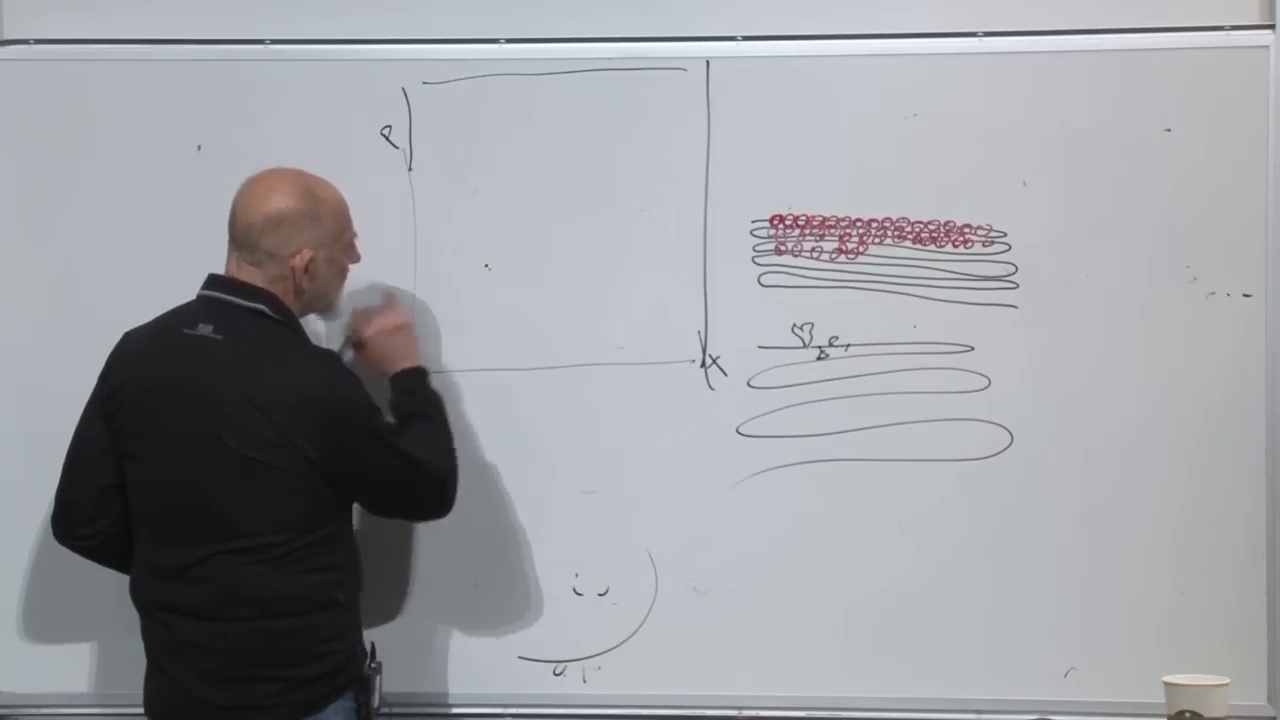
\includegraphics[width=0.90\textwidth]{lecture_07_figure_13.png}
\caption{フィラメントとその粗視化された表現に隣接する、有界な到達可能相空間領域。}
\lectureframe{01:28:10}
\end{figure}

カオス系における近接した初期点は、しばらくは似た履歴をたどるが、その後分離する。ビリヤードのブレイクでは、手球の方向の知覚できないほどの変化がその後の衝突へと写し取られ、差異は複合して最終的な配置が無関係になるまで増大する。したがって、初期のパッチ全体が到達可能領域を通して引き伸ばされ、折り畳まれる。有限の分解能のもとでは、それは広く、ほぼ一様な平衡の記述に近づく。

\begin{figure}[t]
\centering
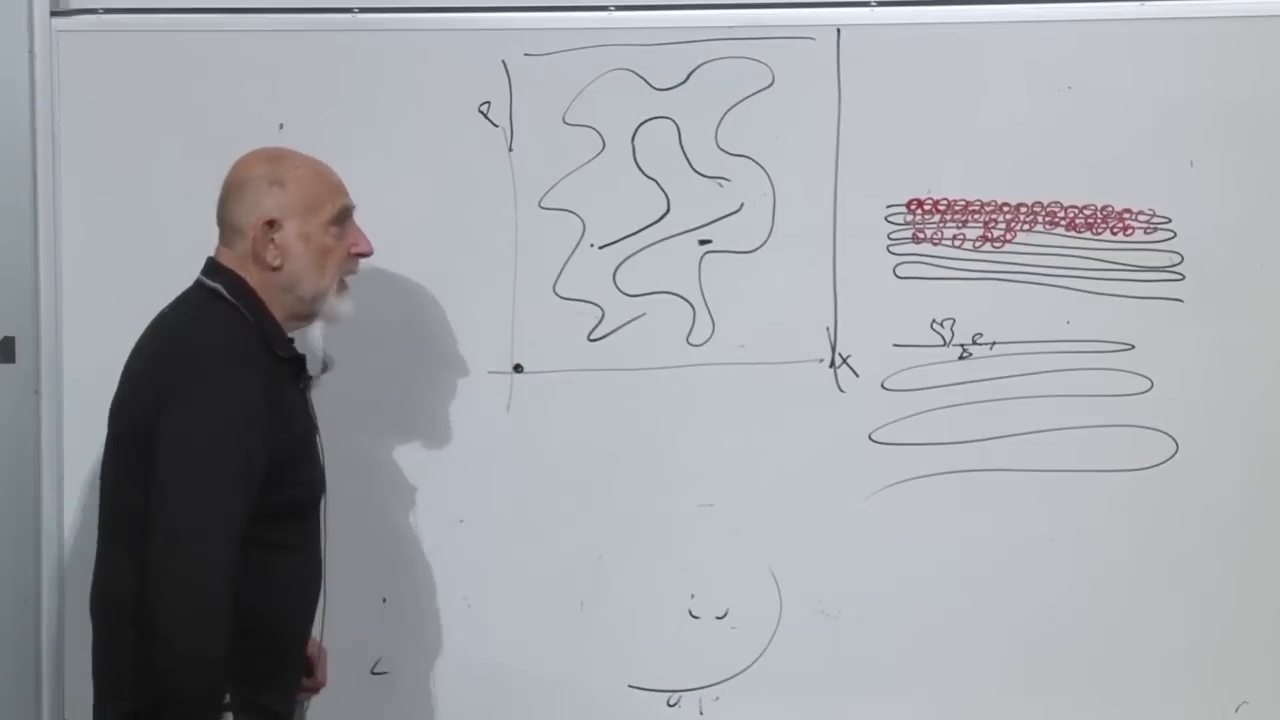
\includegraphics[width=0.90\textwidth]{lecture_07_figure_14.png}
\caption{コンパクトな特別な状態が、有界な到達可能領域を通して複雑なフィラメントへと発展する一方、粗視化されたセルははるかに大きな面積に広がる。}
\lectureframe{01:33:10}
\end{figure}

二つの留保が重要である。カオスそれ自体は、すべての軌道がすべての到達可能な近傍を訪れることを証明しない。そのより強いサンプリングの主張には、エルゴード性または混合性が必要である。また、すべての物理系がカオス的であるわけでもない。一般的な多体系気体と理想化されたビリヤードが意図された設定を与え、そこでは混合性が有用な物理的期待である。

\section{再帰は不可逆性を廃しない}

すべての空気分子が、特別に用意された速度パターンをもって一つの隅から始まるとしよう。衝突はすぐにそれらを部屋中に広げ、粗視化された記述は平衡に達する。有限の測度保存相空間では、ポアンカレの再帰定理は、ほとんどすべての初期点がその出発点にいくらでも近く戻ると述べる。許容誤差\(\epsilon>0\)に対して、再帰時間\(t_R(\epsilon)\)は定理の仮定のもとで有限であるが、巨視的な系では途方もなく大きい。無限に精密な点への厳密な回帰は、必要でもなく、一般に期待もされない。

\begin{classroomqa}
\audiencequestion{ビリヤードの例では、手球を突くことはエネルギーを注入し、閉じた発展を損なうのではないか。}
\lecturerresponse{選ばれた初期状態は、そのエネルギーがすでに含まれた状態で、突いた直後から始まる。再帰はその後の孤立した理想化されたビリヤード力学に関わり、初期状態の近くへの回帰は、選ばれた許容誤差の範囲内で手球がラックに近づくことに相当する配置を含む。
\lecturetimestamp{01:35:37--01:35:55}}
\end{classroomqa}

\begin{classroomqa}
\audiencequestion{気体がやがて隅に戻りうるならば、われわれは情報を失ったのか、そして系は本当に可逆なのか。}
\lecturerresponse{微視的力学は全体を通じて可逆のままである。粗視化エントロピーは、われわれが細かな相関を分解するのをやめるために上昇しうるが、きわめて稀な揺らぎは系をその特別な初期マクロ状態の近くへ戻しうる。したがって、再帰と粗視化された不可逆性は両立する。
\lecturetimestamp{01:37:34--01:38:15}}
\end{classroomqa}

これがボルツマンの本質的な定式化へと導く。エントロピーは論理的に可能なあらゆる瞬間に増大するわけではない。大きな系の非平衡マクロ状態が与えられると、圧倒的に多くの両立する微視的継続は、より特別なものへ向かうよりも、より大きなマクロ状態へ向かう。エントロピーは\emph{おそらく}増大する。下方への揺らぎと再帰は許されるが、その確率と時間スケールは、通常の巨視的経験においてそれらを見えなくする。可逆性の問題は統計力学の偉大な歴史的苦闘の一つであり、ボルツマンに重くのしかかった。その歴史的つながりは、彼の生涯についての単純な因果的主張に変えられるべきではない。

\section{カオスが意味するもの}

より操作的なカオスの定義としては、二つの初期位相点が\(\delta\Gamma(0)\)だけ異なるとき、カオス的な方向は典型的には、線形化された分離が意味を持つ領域で
\begin{equation}
 \lVert\delta\Gamma(t)\rVert
 \sim e^{\lambda t}\lVert\delta\Gamma(0)\rVert,
 \qquad \lambda>0,
 \label{eq:sm7-lyapunov-growth}
\end{equation}
となる。数\(\lambda\)はリアプノフ指数である。時間\(t\)を予測するには、初期データに必要な精度はおよそ\(e^{-\lambda t}\)でスケールする。力学法則の精度も重要である。モデルの誤差は初期条件の誤差とともに増幅される。天気はよく知られた例である。

\begin{classroomqa}
\audiencequestion{\emph{ほとんどの}系がカオス的であると言う原理は存在するのか、それともそれは単に経験的なものなのか。}
\lecturerresponse{カオス的および非カオス的なハミルトニアンは無限に存在し、そもそも\emph{ほとんど}という語にはハミルトニアンの空間上の測度が必要である。複雑な相互作用系はしばしばカオス的であるが、すべてのハミルトニアンを目視で分類するような初等的で普遍的な判定法は存在しない。
\lecturetimestamp{01:39:27--01:40:49}}
\end{classroomqa}

\begin{classroomqa}
\audiencequestion{この議論において\emph{カオス的}とは正確には何を意味するのか。}
\lecturerresponse{近接する位相軌道は、長時間予測には初期条件の知識を指数関数的に改善することを要するほど急速に分離する。調和振動子は対照的である。隣接する位相点はともに回転し、近くにとどまる。厳密な二体ケプラー問題も非カオス的であるが、一般の三体問題にはカオス的な領域がある。
\lecturetimestamp{01:40:50--01:43:45}}
\end{classroomqa}

\begin{classroomqa}
\audiencequestion{運動法則も初期条件と同様に高い精度で知られていなければならないのか。}
\lecturerresponse{はい。両方の誤差源が力学を通じて伝播し、カオス的発展は両方を増幅する。
\lecturetimestamp{01:43:46--01:43:55}}
\end{classroomqa}

二重振り子は鮮やかな例を与える。通常の振り子は可積分で予測可能である。二つ目の振り子を加えると、ほとんど同時に始まった軌道が最終的には異なる仕方でエネルギーを移動し、まったく異なる方向へ向かうことがある。

\begin{figure}[t]
\centering
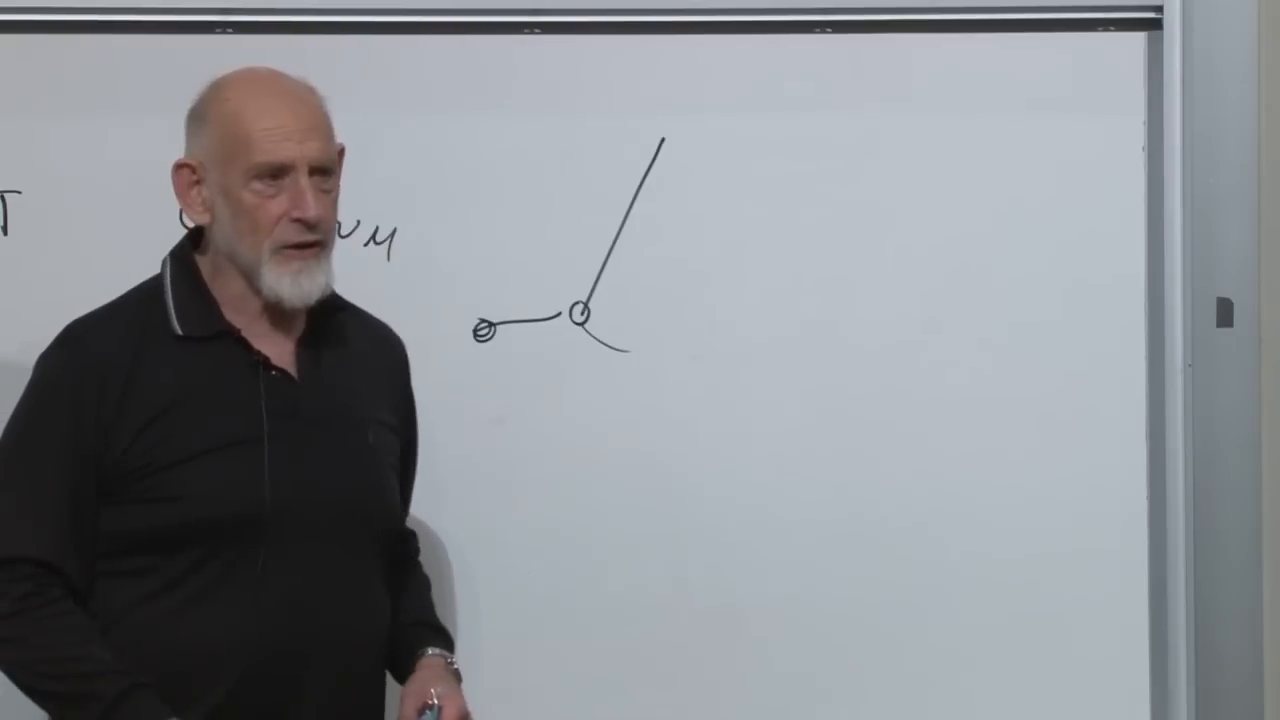
\includegraphics[width=0.90\textwidth]{lecture_07_figure_15.png}
\caption{決定論的カオスの具体例としての二重振り子。}
\lectureframe{01:44:40}
\end{figure}

\begin{classroomqa}
\audiencequestion{なぜある力学系はカオス的であり、別の系はそうでないのか。}
\lecturerresponse{それはハミルトニアンとその不変構造の性質であり、摩擦や実験ノイズの結果ではない。それを決定することは数学的に困難でありうる。複雑さは示唆的であるが証明ではない。
\lecturetimestamp{01:44:03--01:45:58}}
\end{classroomqa}

\begin{classroomqa}
\audiencequestion{摩擦のない理想的な二重振り子も依然としてカオス的か。}
\lecturerresponse{はい。散逸は必要でない。厳密な決定論的ハミルトニアン運動は初期条件への敏感な依存性を持ちうる。無限精度の初期データがあれば軌道は無限に決定されるが、有限精度では予測の地平は有限である。
\lecturetimestamp{01:45:57--01:47:54}}
\end{classroomqa}

\begin{classroomqa}
\audiencequestion{カオスは閉形式解を持たないことと同じか。}
\lecturerresponse{いいえ。カオス系は一般に大域的に有用な閉形式の軌道を持たないが、解析的可解性と敏感な依存性は異なる性質である。カオスは単に公式を書けないことによってではなく、軌道の分離によって力学的に診断される。
\lecturetimestamp{01:48:20--01:49:23}}
\end{classroomqa}

\begin{classroomqa}
\audiencequestion{遍在するカオスは、丘の不安定な頂上で正確に釣り合うこととどう異なるのか。}
\lecturerresponse{丘の頂上は一つの例外的な不安定状態である。そこから離れれば、近接する軌道が急速に分離する必要はない。カオス的領域では、不安定性は軌道に沿って典型的であり、近接する位相点は繰り返し分離する。正のリアプノフ指数がその持続的な成長を捉えている。
\lecturetimestamp{01:49:27--01:50:11}}
\end{classroomqa}

\section{微視的運動から統計法則へ}

音速の見積もりは、微視的な熱運動が巨視的な伝播スケールをどのように定めるかを示し、またその問いは指定されなければならない熱力学的導関数を明らかにした。次に振動子は、古典的等分配の到達範囲と失敗を示した。量子準位間隔は硬いモードを凍結させ、熱容量が温度とともに変化する理由を説明し、無限に多くの高周波モードが無限の熱エネルギーを運ぶことを防ぐ。

厳密な微視的物理から有効な巨視的記述への同じ進行が、第二法則の核心にある見かけの矛盾を解決する。ハミルトン流は厳密な位相空間体積を保存し、可逆のままである。カオス的伸長は巨視的記述が保持するよりも細かい相関を生み出すため、粗視化された占有領域は成長する。再帰は稀な回帰が禁じられていないことを保証する。確率は、なぜそれらが通常の経験を定義しないのかを説明する。第二法則は新しい不可逆的な微視的力ではない。それは、膨大な数の自由度を持つ系における特別な巨視的初期条件に対する、圧倒的に信頼できる統計的な進化の方向である。
\chapter{再帰、非平衡秩序、イジングスピン}

\lectureoverview{部屋の半分から放出された気体は平衡へと急速に進むが、可逆的な力学によれば、十分に長い時間発展は例外的な状態への回帰もまた生じなければならない。我々は相空間体積から回帰時間を見積もり、再帰を宇宙の説明されない低エントロピーな始まりから切り離し、そこから生じる難題を用いてボルツマン脳、整合的な歴史、エネルギー流によって維持される生命について議論する。次に磁気秩序へと移る。独立な二状態スピンは厳密に解ける準備運動を与える。組み合わせ論が分配関数を決定し、磁化は双曲線正接となる。隣接相互作用がついにアップ--ダウン対称性を回復し、一次元イジング模型へと導く。}

\section{やがて戻ってくる部屋いっぱいの空気}

部屋の左半分にすべての空気がある状態から始める。この状態は仕切りによって用意できる。右半分を真空にし、空気を左側に置き、その後壁を取り除く。気体は部屋中に急速に広がり、熱平衡に近づく。エントロピーは増大する。驚くべきことは何も起こっていない。

次に部屋を密閉したまま待つ。百万回連続の表は極めて起こりにくいコイントスの記録であるが、無期限に繰り返される実験はやがて極めて起こりにくい記録を生み出す。同じ論理が気体にも当てはまる。遠いある時刻に、その分子のすべてが再び左半分に、あるいは同程度に特別な領域に見出されるであろう。そのような回帰がポアンカレ再帰である。

正確な定理はこの描像よりやや慎重である。力学が相空間体積を保存する有限測度の相空間領域に対して、ほとんどすべての初期点はその出発点にいくらでも近く戻る。\emph{すべての分子が左半分にある} といった巨視的な言明はより容易である。それは軌道が有限の粗視化された領域に再び入ることだけを問い、すべての分子座標が正確に戻ることを要求しない。実際的な問題は、それにどれだけの時間がかかるかである。

\subsection{高次元の相点}

\(N\) 個の古典粒子に対して、相空間は \(6N\) 個の座標をもち、
\begin{equation}
 \Gamma=(\bm x_1,\ldots,\bm x_N;\bm p_1,\ldots,\bm p_N).
 \label{eq:sm8-phase-point}
\end{equation}
位置は部屋によって有界である。固定された全エネルギーでは、運動量もまた有界である。なぜなら、一つの粒子が任意に大きなエネルギーを運ぶことなく任意に大きな運動量を運ぶことはできないからである。したがって、許されるエネルギー殻は再帰の議論の仮定の下で有限の測度をもつ。

相点は決定論的に運動するが、多体系の気体ではその運動はカオス的である。ビリヤード球の衝突の連続におけるように、近くの軌道は速やかに分離する。粗視化の後、長い軌道はアクセス可能な領域全体をさまようように見える。

\begin{figure}[t]
\centering
\includegraphics[width=0.90\textwidth]{lecture_08_figure_02.png}
\caption{模式的な相空間領域とその中をさまよう複雑な軌道。図は意図的に低次元であり、実際の気体は \(6N\) 次元空間に存在する。}
\lectureframe{00:06:41}
\end{figure}

低次元のスケッチは直ちに我々を誤りへと誘う。特別な状態が描かれた長方形の半分を占めるなら、気体はその時間の半分をそこで過ごすべきだと言うかもしれない。しかし \emph{すべての分子が左半分にある} という条件は、相点の一つの座標だけでなく、すべての位置座標を拘束する。

一次元空間を運動する二つの粒子だけを考え、座標を \(x_1\) と \(x_2\) とする。それらの配置空間は正方形である。\(x_1<L/2\) を要求すると正方形の半分が選ばれ、\(x_1<L/2\) と \(x_2<L/2\) の両方を要求すると四分の一が選ばれる。
\begin{equation}
 P_2=\frac{1}{2}\frac{1}{2}=\frac{1}{4}.
 \label{eq:sm8-two-particle-quarter}
\end{equation}

\begin{figure}[t]
\centering
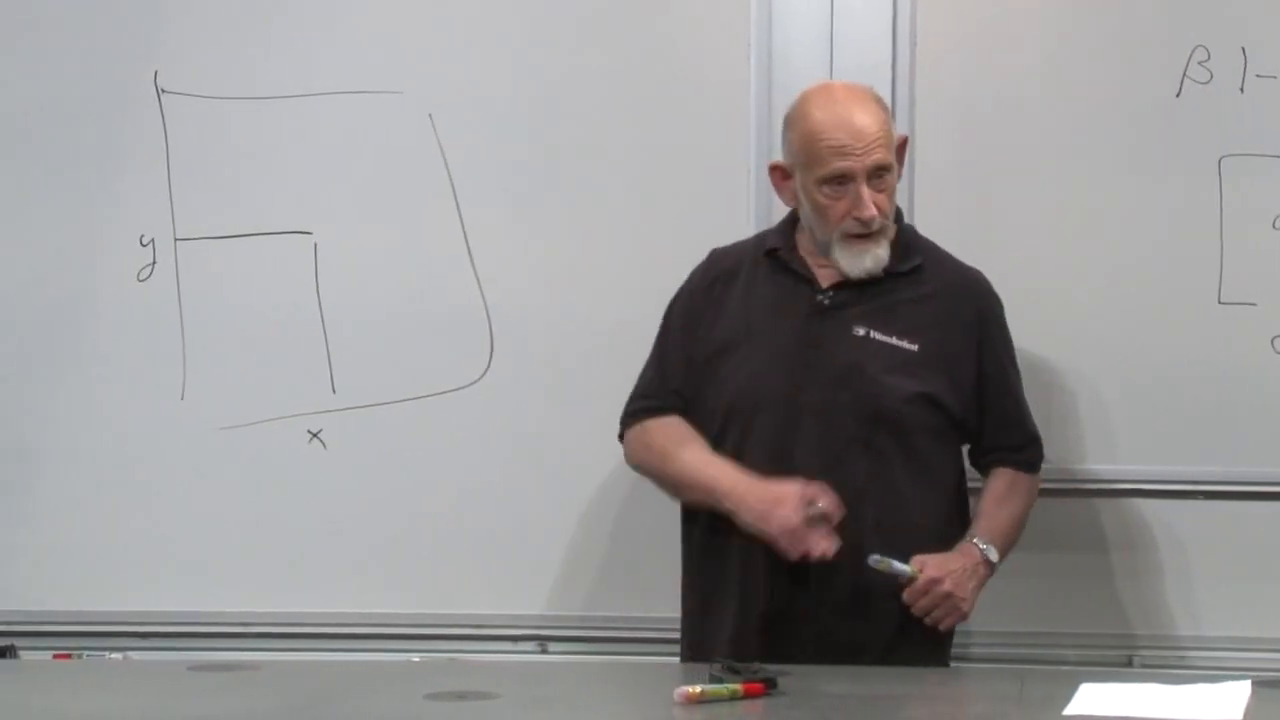
\includegraphics[width=0.90\textwidth]{lecture_08_figure_07.png}
\caption{二つの一次元粒子に対して、より小さな正方形は両方の座標が部屋の選ばれた半分にある配置を表す。}
\lectureframe{00:07:08}
\end{figure}

三つの粒子では \(1/2^3\) となり、\(N\) 個の粒子では
\begin{equation}
 P_{\mathrm{half}}(N)
 =\left(\frac{1}{2}\right)^N.
 \label{eq:sm8-half-probability}
\end{equation}
指数がすべての要点である。二分の一という因子は普通である。巨視的な粒子数で二分の一を累乗したものは、普通の直観を超えている。

\begin{classroomqa}
\audiencequestion{分子は他の空間方向ももつので、答えは \(1/3^N\) であるべきか。}
\lecturerresponse{それは課される条件に依存する。唯一の問いがすべての粒子が仕切りの左側にあるかどうかであるなら、各粒子は一つの二値条件を満たし、答えは \(2^{-N}\) である。利用可能な位置空間の別の独立な割合を拘束すれば、別の因子が与えられる。
\lecturetimestamp{00:07:47--00:08:05}}
\end{classroomqa}

\section{相体積、エントロピー、再帰のスケール}

同じ見積もりは、半分という言い方を参照せずに書くこともできる。部屋が通常の空間体積\(V\)を持ち、\(v\)を、すべての分子が見出されることを要求するより小さな領域とする。二つのマクロ状態に共通な運動量因子を無視すると、利用可能な配置空間体積は
\begin{equation}
 \Omega_{\mathrm{room}}\propto V^N,
 \qquad
 \Omega_{\mathrm{small}}\propto v^N.
 \label{eq:sm8-config-volumes}
\end{equation}
である。したがって、小さなマクロ状態に費やされる長時間の割合は
\begin{equation}
 P(v)
 =\frac{\Omega_{\mathrm{small}}}{\Omega_{\mathrm{room}}}
 =\left(\frac{v}{V}\right)^N.
 \label{eq:sm8-volume-ratio}
\end{equation}
となる。

\begin{figure}[t]
\centering
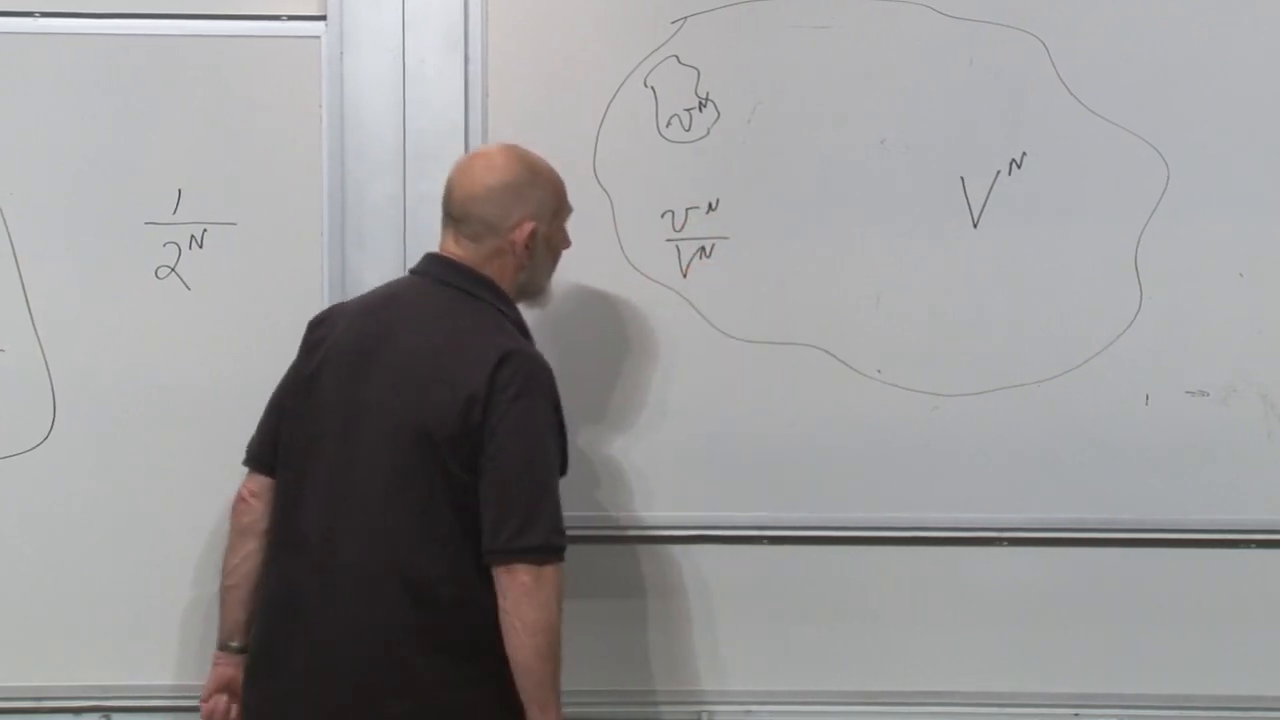
\includegraphics[width=0.90\textwidth]{lecture_08_figure_08.png}
\caption{黒板の一般的な相体積の描像：アクセス可能な領域\(V^N\)の内部にある小さな領域\(v^N\)があり、その比は\(v^N/V^N\)である。}
\lectureframe{00:10:44}
\end{figure}

\(k_B=1\)とする単位系では、エントロピーはアクセス可能な相体積の対数である。\(S_A=\log\Omega_A\)を拘束されたマクロ状態のエントロピー、\(S_{\rm eq}=\log\Omega_{\rm eq}\)を平衡状態のエントロピーとすると、
\begin{equation}
 \begin{aligned}
 P(A)
 &=\frac{\Omega_A}{\Omega_{\rm eq}}\\
 &=\exp\!\left(S_A-S_{\rm eq}\right)\\
 &=e^{-\Delta S},\\
 \Delta S&=S_{\rm eq}-S_A.
 \end{aligned}
 \label{eq:sm8-entropy-probability}
\end{equation}
である。半部屋状態では\(\Delta S=N\log 2\)であり、\eqref{eq:sm8-entropy-probability}は正確に\(2^{-N}\)に帰着する。略記\(P\sim e^{-S_{\rm eq}}\)が適切なのは、特別な領域のエントロピーを固定された基準として扱っている場合だけであり、物理的に意味のある指数はエントロピー欠損\(\Delta S\)である。

\begin{classroomqa}
\audiencequestion{これは相空間全体ではなく配置空間の体積なのか。}
\lecturerresponse{この比較に関しては、そのとおりである。位置に関する条件を課しながら、運動量分布は同じ温度のままにしているので、共通の運動量空間因子は相殺される。完全に一般的な再帰の記述は相空間を用いるが、この特定の確率は配置空間の比から計算できる。
\lecturetimestamp{00:11:21--00:11:40}}
\end{classroomqa}

系がその詳細な位置についての記憶を、微視的な相関時間または混合時間\(\tau_{\rm mix}\)で失うとしよう。そのとき、確率\(P(A)\)の稀な領域は
\begin{equation}
 \tau_{\rm rec}
 \sim \frac{\tau_{\rm mix}}{P(A)}
 \sim \tau_{\rm mix}e^{\Delta S}.
 \label{eq:sm8-recurrence-time-general}
\end{equation}
の尺度で遭遇される。半部屋条件では、
\begin{equation}
 \tau_{\rm rec}\sim\tau_{\rm mix}2^N.
 \label{eq:sm8-recurrence-time-half}
\end{equation}
である。講義では、意図的に粗い部屋サイズの見積もり\(N\sim10^{30}\)を用いており、記憶に残る尺度
\(\tau_{\rm rec}/\tau_{\rm mix}\sim2^{10^{30}}\)
が得られる。通常の大気密度では、部屋は\(10^{27}\)個の分子に近いが、\(10^{30}\)を\(10^{27}\)に置き換えても結論は何も変わらない。再帰時間は宇宙の年齢よりも想像を絶するほど大きいままである。

\begin{classroomqa}
\audiencequestion{再帰時間はどのような単位で測られるのか。秒から時間へ、あるいは極端に短い単位へ変えると、結論は変わりうるのか。}
\lecturerresponse{次元を持つ前因子は\(\tau_{\rm mix}\)であり、巨大な数は無次元の比\(\tau_{\rm rec}/\tau_{\rm mix}\)である。秒を時間に変えることは通常の換算因子で割ることであり、それは\(2^{10^{30}}\)に比べて無視できる。隅への個々の訪問の継続時間は分子速度に依存する。この見積もりが関わるのは、その訪問がどれほど稀に始まるかである。量子再帰定理も存在するが、ここでは必要ない。
\lecturetimestamp{00:17:24--00:19:18}}
\end{classroomqa}

\begin{classroomqa}
\audiencequestion{どの実験も待つことなど到底できない時間を計算する目的は何か。}
\lecturerresponse{要点は概念的である。それは、閉じた力学系がどのような意味で可逆性を保つかを教えてくれる。系はほとんどすべての時間を平衡状態の近くで過ごすが、十分に長い尺度では、より低いエントロピーへ向かう揺らぎも起こす。したがって第二法則は、特別な初期データについての圧倒的に確からしい主張であり、逆向きの運動を禁じる微視的方程式ではない。
\lecturetimestamp{00:15:12--00:16:35}}
\end{classroomqa}

\section{可逆性と特別な始まり}

意図的に、小さな半部屋領域から始める。隣接するほとんどすべての軌道は直ちにそこを離れる。なぜなら、内部よりも外部のはるかに多くの相体積が存在するからである。気体は速やかに広がり、その後、戻るまでに途方もない時間を待つ。速やかな緩和と長い待ち時間の間のこの非対称性は、可逆的な力学に反しない。

速やかな脱出の時間反転は、待ち時間全体ではない。それは、平衡状態に見える分子速度がたまたま整い、気体が部屋の半分へ\emph{swooshes}と流れ込む、短く、驚異的にうまく調整されたエピソードである。通常の脱出の終わりにすべての運動量を反転させれば、気体は脱出を逆向きにたどる。長い待ち時間とは、その特別な入射速度パターンが自発的に生じるのに必要な時間である。

\begin{classroomqa}
\audiencequestion{時間対称性とは、隅への遅い再帰が、そこからの元の脱出と同じだけ長くかかることを意味するのか。}
\lecturerresponse{いいえ。脱出をその正確な時間反転と比較せよ。どちらも速やかである。膨大な時間がかかるのは、逆向きの流れ込みを開始させる正確な入射揺らぎを、平衡状態で待つことである。途方もなく長い記録の上では、平衡から離れる逸脱は、対称な局所履歴をもって両方の時間方向に起こる。
\lecturetimestamp{00:20:46--00:21:58}}
\end{classroomqa}

したがって、再帰の議論は時間の矢の一部しか説明しない。系が低エントロピーの領域から始まった\emph{という条件のもとで}、エントロピーが通常は増大する理由を説明する。しかし、初期条件がなぜ特別であったかは説明しない。宇宙論では、この欠けた前提が中心的な問いとなる。なぜ観測可能な宇宙は、その重力相空間のこれほど例外的に小さな領域から始まったのか。

\begin{classroomqa}
\audiencequestion{再帰は宇宙論に当てはまるか。宇宙が広がった後、十分長く待てば再帰するのだろうか。}
\lecturerresponse{その問いは避けられないが、その答えは大域的な宇宙論に依存する。有限の平衡状態空間をもつ真に閉じた系は再帰を促す。膨張する時空、重力、地平線、そして無限または非定常な状態空間は前提を変えうる。ここでの重要な教訓はより限定的である。平衡の再帰という描像それ自体は、我々が見る構造化された宇宙に対する満足な統計的説明ではない。
\lecturetimestamp{00:19:59--00:20:45}}
\end{classroomqa}

\begin{classroomqa}
\audiencequestion{再帰は、最初に気体を小さな領域に用意することに依存するのか。部屋が平衡から始まっても、空気は最終的にやはり一つの隅に集まるのか。}
\lecturerresponse{はい。再帰は閉じた系の長時間の力学に関するものであるから、平衡に見える初期状態もまれな低エントロピー揺らぎを経る。半部屋状態を用意することが重要であるのは別の理由による。それにより、既知の特別な始まりを条件として、その直後にエントロピーがなぜ増大するのかを問うことができる。
\lecturetimestamp{00:22:04--00:22:20}}
\end{classroomqa}

\section{なぜランダムな揺らぎは少なすぎることを予測するのか}

再帰を宇宙論に変えようとする試みもありうる。おそらく宇宙は永遠のほとんどを平衡で過ごし、我々の現在の世界はまれな一つの揺らぎなのだろう。この提案は鋭い統計的検証に失敗する。観測者が存在することを条件として、その観測者が他に何を見ることを期待すべきかを問うのである。

一つの惑星を作るのに十分大きな揺らぎは、極めてまれである。二つの惑星を作る揺らぎは、より大きなエントロピー不足を必要とし、さらにまれである。恒星、銀河、宇宙マイクロ波背景放射、そして長い過去について互いに整合する記録を作る揺らぎは、莫大な追加の指数分だけさらにまれである。したがって、平衡揺らぎ理論は、観測に十分な最小の揺らぎを予測するのであって、実際に観測される豊かに整合した世界を予測するのではない。その最も極端な形では、最小の観測者はボルツマン脳と呼ばれる。

論理は条件付き確率である。\(A\)を観測者サイズの揺らぎが一つ起こる事象、\(B\)を独立な第二の構造とする。両者が微小な確率\(p\)をもつならば、
\begin{equation}
 P(B\mid A)=p,
 \qquad
 P(A\cap B)=p^2.
 \label{eq:sm8-conditional-fluctuations}
\end{equation}
第一の揺らぎが起こったことを知っても、第二の揺らぎが起こりやすくなるわけではない。宝くじの類推はこの水準では正確である。以前の当選者は、次の独立な抽選で当たる確率が高くなるわけではない。したがって、観測者は自分が存在することを条件としてよいが、独立に構造化された環境を見いだしたならば、それでも驚くべきである。

\begin{classroomqa}
\audiencequestion{一つの惑星または一人のボルツマン観測者がすでに存在するとして、もう一つが存在する確率は本当に小さいのか。}
\lecturerresponse{第二の独立なまれな揺らぎに対する条件付き確率は、同じ微小な一事象確率であり、その二乗ではない。両方に対する同時確率が二乗である。まさにこの理由により、第一の観測者は自分の外側には依然として熱的無秩序を期待すべきである。配偶者、別の惑星、そして秩序だった空を見いだすことは、その観測者が孤立した平衡揺らぎとして組み立てられたという前提に反する証拠である。
\lecturetimestamp{00:26:12--00:30:27}}
\end{classroomqa}

\subsection{過去についての整合する記録}

同じ議論は歴史にも当てはまる。一致する二冊の教科書、一つの膨張史に適合する天文記録、地質層、記憶、実験ノートはすべて互いを制約する。一冊のランダムな教科書はどんな物語でも含みうる。同じ過去について一致する記録の網全体は、はるかに小さな相空間領域を占める。

教室の例では、ジョージ・ワシントンが桜の木を切り倒したというよく知られた話を用いる。その話が真実かどうかは無関係である。要点は、現在の瞬間に揺らぎから存在するに至った世界では、ある本の一文が別の記録の一致に対する力学的な理由を与えないということである。整合する相関は、単なる一瞬の偶然の証拠ではなく、共有された歴史の証拠である。

\begin{classroomqa}
\audiencequestion{ここでいう\emph{歴史的一貫性}とは何を意味するのか。}
\lecturerresponse{それは、現在の多くの記録が共通の過去の帰結として互いに整合していることを意味する。揺らぎが記録や記憶を捏造することはあり得るが、相互に整合するネットワークを捏造するには、最小限の観測者を一つ捏造するよりもはるかに大きな揺らぎが必要である。したがって再帰理論は、観測者に似た揺らぎの大多数は、我々が実際に見出している一貫性を欠くと予測する。
\lecturetimestamp{00:30:30--00:31:12}}
\end{classroomqa}

\begin{classroomqa}
\audiencequestion{宇宙は依然として閉じた系であり、その平衡化時間と再帰時間が単に極めて長いだけだということはあり得ないのか。}
\lecturerresponse{その可能性は統計的な問題を取り除かない。無限に長い歴史の上では、観測者に似た揺らぎが多数存在し、その圧倒的多数は一貫した周囲の歴史を伴わない最小限のものであろう。その集団から選ばれた観測者は、我々の観測を期待すべきではない。したがって宇宙論研究者は、ボルツマン脳問題を、再帰がすでに観測されたという主張としてではなく、宇宙論的測度と晩期モデルの検証として真剣に受け止めている。
\lecturetimestamp{00:31:13--00:32:42}}
\end{classroomqa}

\section{流れによって維持される構造としての生命}

生命は逆の困難を提起しているように見える。生物は複雑な組織を長期間維持するのであり、短命的な偶発的揺らぎのようには見えない。その解決は、第二法則が完全な閉じた系に適用されるということである。部分系は、その環境においてより大きなエントロピー増大が起こるならば、そのエントロピーを低下させ、あるいは維持してもよい：
\begin{equation}
 \dot S_{\rm total}
 =\dot S_{\rm subsystem}+\dot S_{\rm environment}\geq 0.
 \label{eq:sm8-open-system-second-law}
\end{equation}

地球は熱平衡にはない。人間の時間尺度ではほぼ定常であるが、定常は静的を意味しない。エネルギーが地球を通って流れる。太陽光が到来し、多くの過程を通じて劣化し、より低い実効温度で放射されて去る。その通過流量は、全エントロピーが増大しつつ局所的な組織を維持し得る。

管を通って流れる水は、直接的な力学的イメージを与える。その流れは持続的な渦や渦巻きを含み得る。それらは組織化された構造であるが、水流によって維持されている。両端を密閉し、流れを止めれば、水が鈍い平衡に近づくにつれて粘性が渦を消し去る。流出する水は流入する水より温かいので、より大きな系がエントロピーの勘定を支払ったことになる。

\begin{classroomqa}
\audiencequestion{生命はエントロピーを減少させるのか、そしてなぜその組織は通常の揺らぎのように現れては消えるのではなく持続し得るのか。}
\lecturerresponse{生命は局所的にエントロピーを維持し、あるいは低下させ得るが、それはさらに多くのエントロピーを外部へ排出することによってのみである。その持続は定常的な非平衡の流れ、主に地球を通る太陽エネルギーの流れに由来する。もし地球が入射および出射放射に対して密閉されていれば、やがて熱平衡に近づき、組織化された活動は停止するであろう。生命は平衡の揺らぎというよりも、流れの中の渦に近い。
\lecturetimestamp{00:32:43--00:35:42}}
\end{classroomqa}

これで我々は\emph{興味深いもの}を離れ、講義の意図的に乾いた表現を借りれば、何か退屈なもの、すなわち磁石に戻る。

\section{磁石の冷却：磁区と選ばれた方向}

統計力学は、文字通りの鉄片でない場合でも、数学的模型をしばしば磁石と呼ぶ。有用な共通の特徴は、秩序化し得る局所的自由度の集まりである。実際の磁性材料では、これらの自由度は原子磁気モーメント、電子スピン、軌道電流、または結晶単位の有効モーメントに由来し得る。

高温では熱的無秩序により局所モーメントが多くの方向を向き、正味の磁化はほとんど、あるいは全く生じない。隣接するモーメントが整列したときに低いエネルギーを持つならば、冷却によって小さな整列磁区が形成され得る。さらに冷却するとエネルギーの利得がより重要になり、相関した磁区が成長する。強磁性転移を支える系では、相関長は有限の臨界温度で巨視的になる。すると秩序相は、ゼロ磁場のエネルギーが前もって一つの方向を好まなかったにもかかわらず、一つの配向を選ぶ。

\begin{classroomqa}
\audiencequestion{N極がS極を引き付けるのだから、微視的な磁石は反平行に整列することを好むべきではないのか。}
\lecturerresponse{有効相互作用は物質に依存する。通常の双極子の直観は微視的問題のすべてではない；交換相互作用、結晶構造、競合する相互作用が重要である。強磁性材料とは、有効な低エネルギー傾向が平行秩序を好むものであり、他の材料は反平行整列を好み得る。
\lecturetimestamp{00:39:56--00:40:30}}
\end{classroomqa}

\begin{classroomqa}
\audiencequestion{モーメントが揃うためには、物質が冷却する間に外部磁場が存在しなければならないのだろうか。}
\lecturerresponse{いいえ。相互作用は磁場なしでも秩序を生み出しうる。完全に対称な理想化では、異なる方向はエネルギー的に等価であるため、実現される方向は初期揺らぎ、境界、あるいは任意に小さな迷走磁場によって選ばれる。それらの等価な方向の一つを選ぶことが自発的対称性の破れであり、巨視的秩序の出現が磁気相転移である。
\lecturetimestamp{00:40:31--00:42:33}}
\end{classroomqa}

実在の物質は複雑であるから、ここでは徹底的に単純化する。各局所モーメントは上向きか下向きのいずれかしか向けない：
\begin{equation}
 \sigma_i=+1\quad\hbox{or}\quad\sigma_i=-1.
 \label{eq:sm8-ising-spin}
\end{equation}
この模型には東も西もない。許される二つの配向は、表と裏が硬貨の二つの結果であるのと同様に、模型の定義である。その価値は微視的実在性にあるのではなく、数学的明瞭さと、多くの系に共通する秩序化現象を表現できることにある。

\begin{classroomqa}
\audiencequestion{これら二状態の対象は物理的には何なのか。それらを粒子として想像すべきなのだろうか。}
\lecturerresponse{結晶の格子点にある原子を思い描き、それぞれがスピンや微視的電流によって生じた有効磁気モーメントを持つと考えることができる。しかし模型にとっては、二値変数だけが重要である。上向きと下向きへの制限は、統計力学を簡単にするために課されている。
\lecturetimestamp{00:44:22--00:45:01}}
\end{classroomqa}

\section{外部磁場中の独立スピン}

最初の模型は互いに相互作用しない\(N\)個のスピンを含む。外部磁場\(H\)が唯一のエネルギー尺度を与え、\(\mu\)は一つのスピンのそれへの結合の強さを測る。計算で用いた符号の規約を保つ：
\begin{equation}
 \epsilon_i=\mu H\sigma_i.
 \label{eq:sm8-single-spin-energy}
\end{equation}
\(H>0\)に対して、上向きスピン\(\sigma_i=+1\)はエネルギー\(+\mu H\)を持ち、下向きスピン\(\sigma_i=-1\)はエネルギー\(-\mu H\)を持つ。したがってこの規約では、正の磁場は下向きスピンを好む。これは別の一般的な命名規約とは逆であるが、符号を一貫して用いる限り、名前には物理が依存しない。

\(n\)を上向きスピンの数、\(m\)を下向きスピンの数とする。このとき
\begin{equation}
 n+m=N,
 \qquad
 E=(n-m)\mu H.
 \label{eq:sm8-counting-energy}
\end{equation}

\begin{figure}[t]
\centering
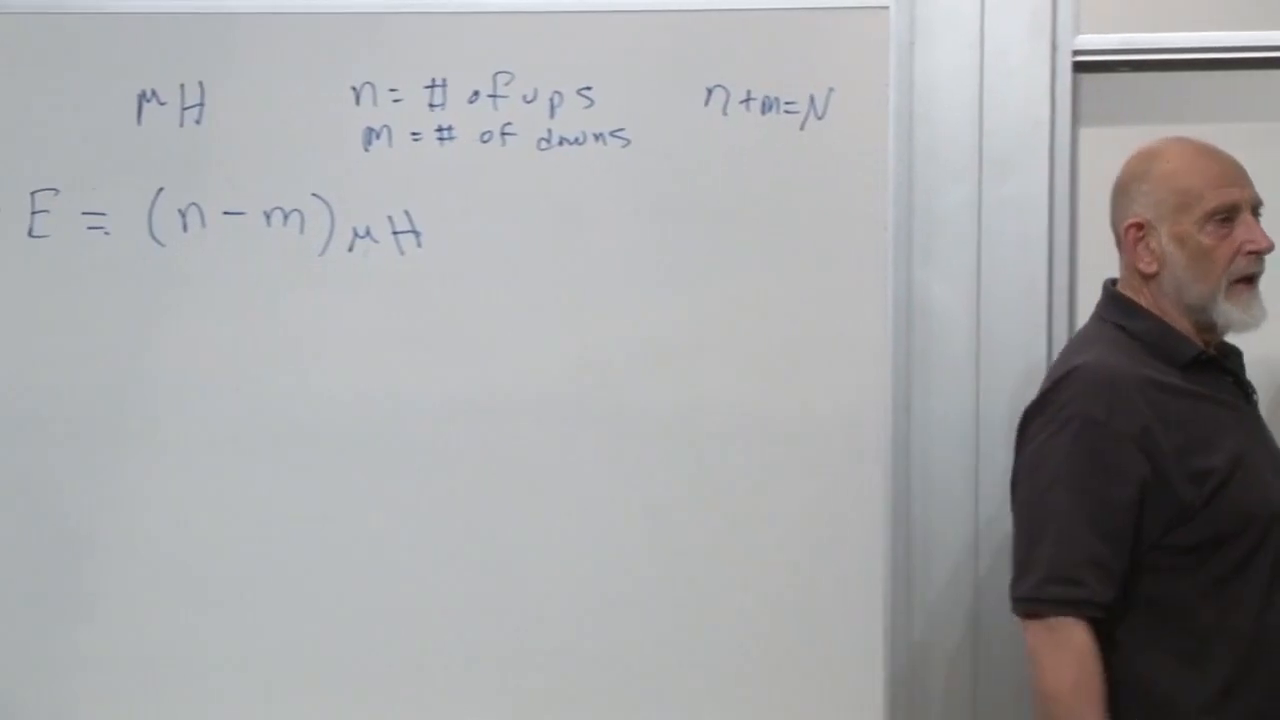
\includegraphics[width=0.90\textwidth]{lecture_08_figure_03.png}
\caption{独立スピンの設定：上向きスピン\(n\)個、下向きスピン\(m\)個、\(n+m=N\)、および\(E=(n-m)\mu H\)。}
\lectureframe{00:49:50}
\end{figure}

\begin{classroomqa}
\audiencequestion{\(H\)、\(\mu\)、\(E\)の次元は何か。\(H\)は数なのか磁場なのか。}
\lecturerresponse{\(H\)は外部から課された磁場の強さを表し、\(\mu\)は磁気モーメントを表す。それらの積\(\mu H\)はエネルギーの次元を持つ。抽象模型では、しばしばそれらを単一のエネルギー値のパラメータにまとめ、慣例的に小文字の\(h\)でも表す。ここではそれらの物理的起源を示すために両方の因子を保ち、\(E\)は全エネルギーである。
\lecturetimestamp{00:48:21--00:49:27}}
\end{classroomqa}

\subsection{配置の数え上げ}

固定された\(n\)と\(m=N-n\)に対して、\(N\)個の格子点のうちどの\(n\)個が上向きであるかを選ぶ。その多重度は
\begin{equation}
 \Omega(n,m)=\binom{N}{n}
 =\frac{N!}{n!\,m!}.
 \label{eq:sm8-spin-multiplicity}
\end{equation}
これらの配置の一つ一つが同じエネルギー
\eqref{eq:sm8-counting-energy}を持つ。

\begin{classroomqa}
\audiencequestion{\(n\)と\(m\)は独立でないのだから、両方を和の添字にできるのか。また組合せ因子はどこで入るのか。}
\lecturerresponse{それらは\(n+m=N\)という拘束された対として書くこともできるし、\(n=0,\ldots,N\)について和をとり\(m=N-n\)と置くこともできる。ボルツマン重みは個々の配置に属し、同じエネルギーの配置をすべてまとめると、その重みに\(N!/(n!\,m!)\)が掛かる。
\lecturetimestamp{00:52:04--00:53:03}}
\end{classroomqa}

したがって分配関数は
\begin{align}
 Z_N
 &=\sum_{n+m=N}
   \frac{N!}{n!\,m!}
   e^{-\beta\mu H(n-m)}
 \notag\\
 &=\sum_{n=0}^{N}
   \binom{N}{n}
   \left(e^{-\beta\mu H}\right)^n
   \left(e^{+\beta\mu H}\right)^{N-n}.
 \label{eq:sm8-spin-z-sum}
\end{align}
次のものを導入する：
\begin{equation}
 x=e^{-\beta\mu H},
 \qquad
 y=e^{+\beta\mu H}.
 \label{eq:sm8-xy}
\end{equation}
二項定理が計算を完成させる：
\begin{align}
 Z_N
 &=\sum_{n=0}^{N}\binom{N}{n}x^n y^{N-n}
   =(x+y)^N
 \notag\\
 &=\left(e^{-\beta\mu H}+e^{+\beta\mu H}\right)^N
   =\left[2\cosh(\beta\mu H)\right]^N.
 \label{eq:sm8-spin-z-closed}
\end{align}

\begin{figure}[t]
\centering
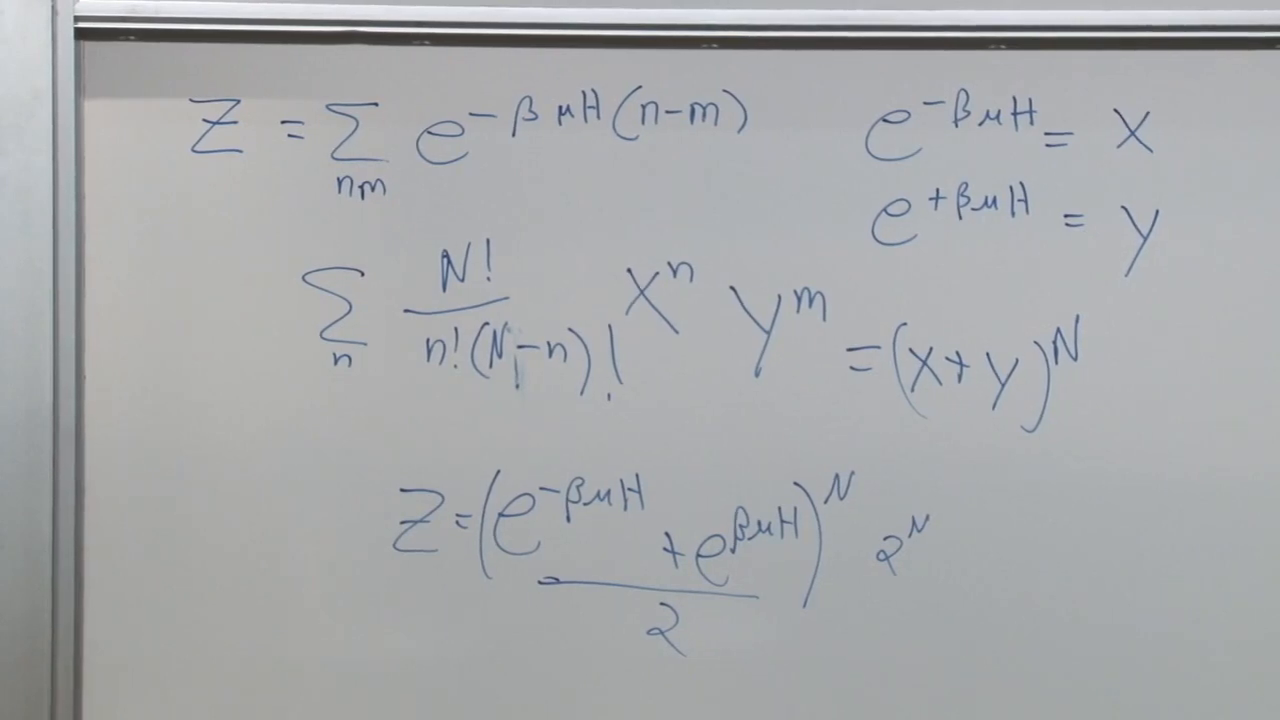
\includegraphics[width=0.90\textwidth]{lecture_08_figure_04.png}
\caption{分配関数の和、置換\(x\)および\(y\)、そして\(2\cosh(\beta\mu H)\)の冪への二項定理による簡約。}
\lectureframe{00:56:00}
\end{figure}

より短い導出もある。スピンは独立であるから、一つのスピンは
\begin{equation}
 z_1=e^{-\beta\mu H}+e^{+\beta\mu H}
    =2\cosh(\beta\mu H),
 \label{eq:sm8-one-spin-z}
\end{equation}
および\(Z_N=z_1^N\)を持つ。それでも組合せによる導出は、多重度がエネルギーとどのように競合するかを明示的に示すので、保持する価値がある。

\section{配置の磁化とアンサンブルの磁化}

一つの配置に対して、そのサイトあたりの無次元スピン過剰を次で定義する：
\begin{equation}
 M_{\rm conf}=\frac{n-m}{N}.
 \label{eq:sm8-config-magnetization}
\end{equation}
これはすべてのスピンが上向きのとき\(+1\)から、すべてのスピンが下向きのとき\(-1\)までの範囲をとる。ここで用いる熱力学的磁化はそのボルツマン平均であり、
\begin{equation}
 M=\left\langle M_{\rm conf}\right\rangle
  =\left\langle\frac{n-m}{N}\right\rangle.
 \label{eq:sm8-average-magnetization}
\end{equation}
因子\(\mu H\)はこの定義に属さない。計算中に一時的にそこに書かれ、その後除かれた。\(\mu H\)はスピン過剰をエネルギーに変換する。

配置ごとに、
\begin{equation}
 E=N\mu H M_{\rm conf}.
 \label{eq:sm8-energy-config-m}
\end{equation}
平均の線形性から直ちに
\begin{equation}
 \langle E\rangle=N\mu H M.
 \label{eq:sm8-energy-average-m}
\end{equation}

\begin{figure}[t]
\centering
\includegraphics[width=0.90\textwidth]{lecture_08_figure_05.png}
\caption{スピンの行、補正された平均磁化、そして黒板で強調されたエネルギー関係。}
\lectureframe{01:01:22}
\end{figure}

\begin{classroomqa}
\audiencequestion{磁化は特定の配置に割り当てられているのか、それとも平均磁化について議論しているのか。なぜ同じ関係が平均エネルギーに対しても成り立つのか。}
\lecturerresponse{両方の概念が現れるが、それらは区別されるべきである。\((n-m)/N\) は一つの配置における値であり、\(M\) はそのボルツマン平均である。\(E=N\mu H M_{\rm conf}\) は各配置で別々に成り立つので、両辺を同じ確率で平均すると \(\langle E\rangle=N\mu H M\) が得られる。固定された量 \(N\)、\(\mu\)、\(H\) は平均の外に出る。
\lecturetimestamp{00:59:54--01:03:40}}
\end{classroomqa}

\begin{classroomqa}
\audiencequestion{どのようにしてモデルは、上向きと下向きの間に偏りを与えることなく、すべてのスピンを北--南に揃えることができるのか。}
\lecturerresponse{東と西が存在しないことは二状態モデルに組み込まれている。それは許される自由度の制限である。現在の外部場モデル \emph{は}上向きと下向きの間に偏りを持つ。我々の符号の規約では、場は下向きスピンのエネルギーを下げる。したがってこのモデルには上--下対称性がない。以下で導入するゼロ場イジング模型がその対称性を回復する。
\lecturetimestamp{01:03:41--01:04:53}}
\end{classroomqa}

\subsection{分配関数からのエネルギー}

平均エネルギーは通常の恒等式から従う。
\begin{equation}
 \langle E\rangle
 =-\frac{\partial}{\partial\beta}\log Z_N.
 \label{eq:sm8-energy-identity}
\end{equation}
\eqref{eq:sm8-spin-z-closed} を用いると、
\begin{align}
 \log Z_N
 &=N\log 2+N\log\!\left[\cosh(\beta\mu H)\right],
 \notag\\
 \langle E\rangle
 &=-N\mu H\,
   \frac{\sinh(\beta\mu H)}{\cosh(\beta\mu H)}
 \notag\\
 &=-N\mu H\tanh(\beta\mu H).
 \label{eq:sm8-average-energy}
\end{align}
これを \eqref{eq:sm8-energy-average-m} と組み合わせると
\begin{equation}
 \boxed{M=-\tanh(\beta\mu H)}.
 \label{eq:sm8-magnetization-tanh}
\end{equation}

答えの形に物理が含まれている。思い出そう。
\begin{equation}
 \cosh x=\frac{e^x+e^{-x}}{2},
 \qquad
 \sinh x=\frac{e^x-e^{-x}}{2}.
 \label{eq:sm8-hyperbolic-definitions}
\end{equation}
原点付近では \(\tanh x=x+O(x^3)\) であり、大きな正の \(x\) に対しては \(1\) に近づく。\(\beta=1/T\) であるから、
\begin{equation}
 M\longrightarrow -1
 \quad (T\longrightarrow0),
 \qquad
 M\longrightarrow 0
 \quad (T\longrightarrow\infty).
 \label{eq:sm8-magnetization-limits}
\end{equation}
ゼロ温度ではすべてのスピンがより低いエネルギーの下向き状態を占める。無限温度ではすべての配置が等しい重みを持ち、場の偏りは洗い流される。\(H\) を反転させると \(M\) が反転する。

\begin{figure}[t]
\centering
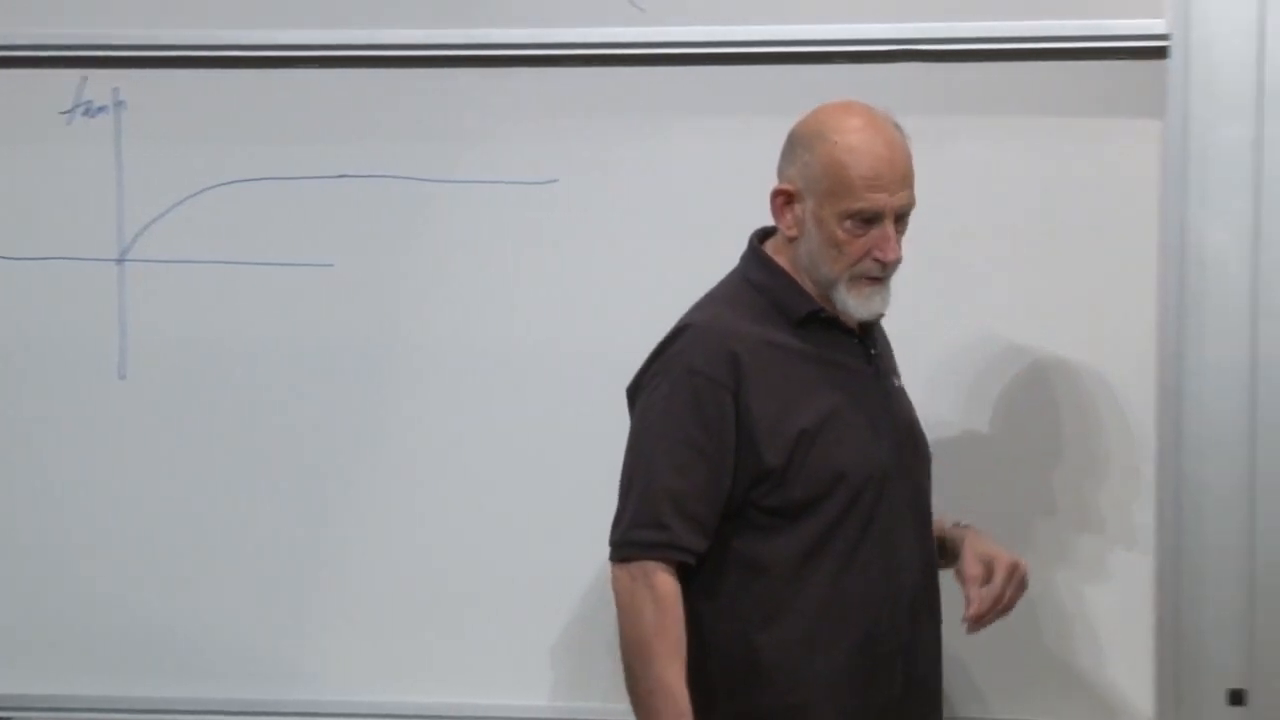
\includegraphics[width=0.90\textwidth]{lecture_08_figure_09.png}
\caption{双曲線正接曲線は大きな \(\beta\mu H\) で一定値に近づき、原点付近では線形である。講義の規約における物理的磁化は、プロットされた \(\tanh\) の負である。}
\lectureframe{01:13:14}
\end{figure}

\begin{classroomqa}
\audiencequestion{磁化は連続的に変化する。先に言及された相転移温度はどこにあるのか。}
\lecturerresponse{このモデルには存在しない。非零の外部場中の独立スピンは単純すぎ、\(\log Z_N=N\log[2\cosh(\beta\mu H)]\) はすべての有限の正の温度で滑らかである。相転移には、今から取り組む相互作用する対称な問題が必要であり、二次元ゼロ場イジング模型が有限温度転移を持つこの族の最初の例である。
\lecturetimestamp{01:14:47--01:15:11}}
\end{classroomqa}

\section{イジング模型：隣接ペアのエネルギー}

外部場は統計が始まる前に方向を選んだ。その場を取り除き、隣接スピンが互いの有効場を提供するようにしよう。あるサイトの両隣が上を向いていれば、それらは上を好む。両方が下を向いていれば、下を好む。一方がそれぞれ逆を向いていれば、最も単純な描像ではそれらの効果は打ち消し合う。エネルギーは今や孤立したサイトではなくペアに結びついている。

二つの隣接スピンに対して、\(J>0\) を選び、
\begin{equation}
 E_{12}=-J\sigma_1\sigma_2.
 \label{eq:sm8-pair-energy}
\end{equation}
と書く。揃ったスピンは \(\sigma_1\sigma_2=+1\) を持ち、エネルギーは \(-J\) である。逆向きのスピンは積 \(-1\) を持ち、エネルギーは \(+J\) である。したがってマイナス符号こそが相互作用を強磁性的にするものである。

\begin{figure}[t]
\centering
\includegraphics[width=0.90\textwidth]{lecture_08_figure_06.png}
\caption{局所強磁性相互作用
\(E_{12}=-J\sigma_1\sigma_2\)。}
\lectureframe{01:19:59}
\end{figure}

開いた一次元鎖ではハミルトニアンは
\begin{equation}
 {\cal H}=-J\sum_{i=1}^{N-1}\sigma_i\sigma_{i+1}.
 \label{eq:sm8-ising-chain-open}
\end{equation}
である。周期境界条件では \(\sigma_{N+1}=\sigma_1\) と置き、\(N\) まで和を取る。どちらの規約でも各隣接ペアを一度ずつ数える。それらの境界の違いは長い鎖では無視できるようになる。

\begin{figure}[t]
\centering
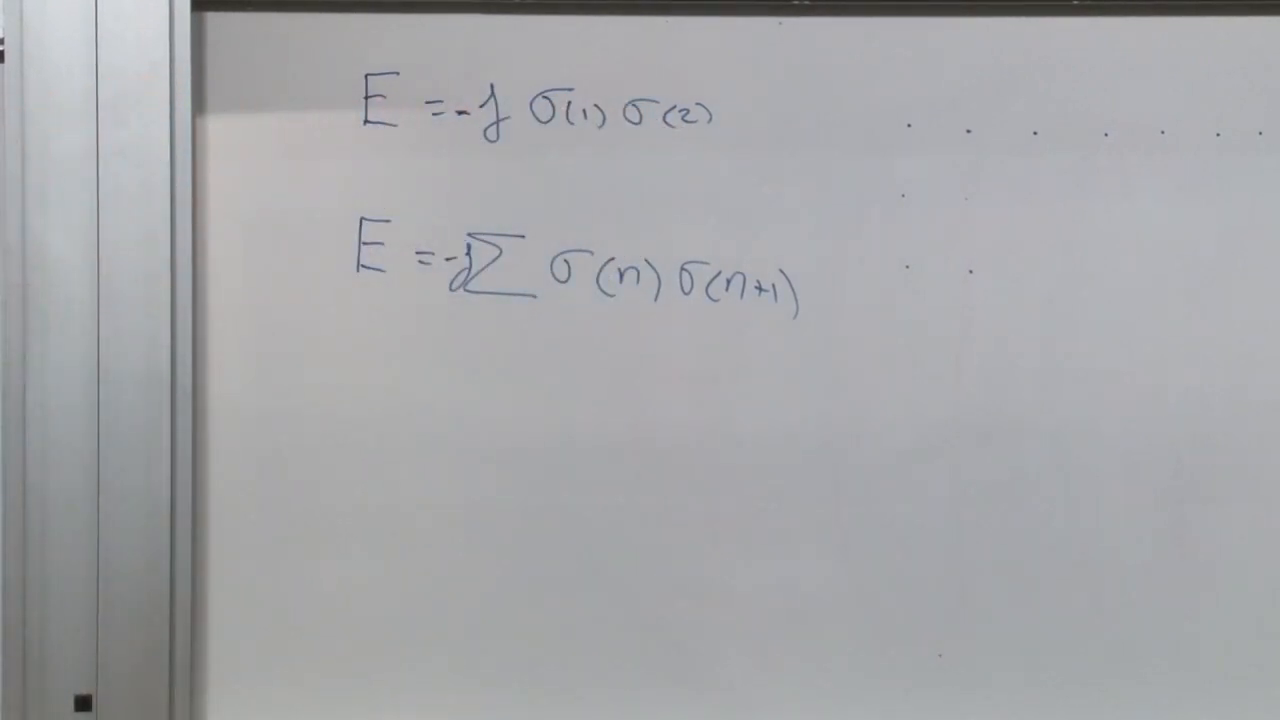
\includegraphics[width=0.90\textwidth]{lecture_08_figure_10.png}
\caption{局所ペアエネルギーを最近接鎖ハミルトニアンに拡張したもの。}
\lectureframe{01:20:46}
\end{figure}

無限温度ではすべてのスピン列が等確率である。平均して結合の半分は揃っており、半分は逆向きであるから、
\begin{equation}
 \left\langle\sigma_i\sigma_{i+1}\right\rangle_{T=\infty}=0,
 \qquad
 \left\langle{\cal H}\right\rangle_{T=\infty}=0.
 \label{eq:sm8-infinite-t-bond}
\end{equation}
ここでのゼロエネルギーは低エネルギー状態ではない。すべて揃った基底状態は結合あたりエネルギー \(-J\) を持つので、無限温度のアンサンブルはそれより示量的なエネルギーだけ上にある。

\begin{classroomqa}
\audiencequestion{個々の積 \(\sigma_i\sigma_{i+1}\) が \(+1\) か \(-1\) のいずれかであるのに、なぜ平均積がゼロになりうるのか。}
\lecturerresponse{平均は単一配置で取られる値の一つである必要はない。無限温度では揃った結合と逆向きの結合が等しい頻度で起こるので、それらの \(+1\) と \(-1\) の寄与は打ち消し合う。磁化で重要だったのと同じ平均の区別がここでも重要である。
\lecturetimestamp{01:21:39--01:22:37}}
\end{classroomqa}

\subsection{二つの基底状態と一つの大域的対称性}

絶対零度では、すべての結合が揃おうとする。したがって二つの基底状態が存在する。
\begin{equation}
 (+,+,+,\ldots,+)
 \qquad\hbox{and}\qquad
 (-,-,-,\ldots,-).
 \label{eq:sm8-two-ground-states}
\end{equation}
これらはまったく同じエネルギーをもつ。ハミルトニアンはこの縮退を明瞭にする。すなわち、すべてのスピンを反転させると、
\begin{equation}
 \sigma_i\longmapsto-\sigma_i
 \qquad\hbox{for all }i,
 \label{eq:sm8-global-flip}
\end{equation}
すべての結合の積は不変である。
\begin{equation}
 (-\sigma_i)(-\sigma_{i+1})
 =\sigma_i\sigma_{i+1}.
 \label{eq:sm8-global-flip-invariance}
\end{equation}
一つのスピンを反転させることは対称性ではない。なぜなら、隣接する結合の積の符号を反転させるからである。すべてのスピンを反転させることは対称性である。これが零磁場イジング模型の大域的\(\mathbb Z_2\)対称性である。

\begin{figure}[t]
\centering
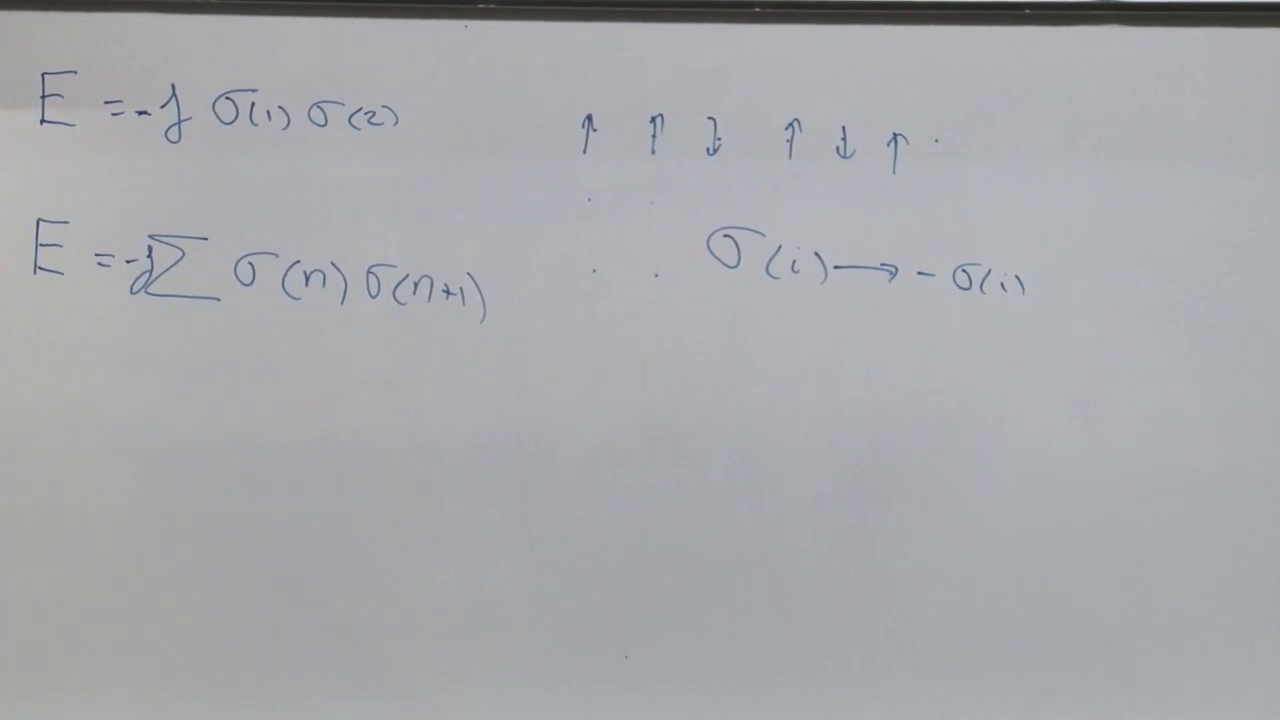
\includegraphics[width=0.90\textwidth]{lecture_08_figure_11.png}
\caption{大域的変換\(\sigma_i\mapsto-\sigma_i\)の隣に置かれた鎖のハミルトニアン。この変換はすべての対の積を不変に保つ。}
\lectureframe{01:26:31}
\end{figure}

厳密に絶対零度において、一つのスピンに微小な磁場を加える。それは二つの基底状態の間の引き分けを破り、強磁性的結合がその選択を鎖全体に伝播させる。状態が選択された後に磁場を取り除くと、大きな系はその配向を非常に長い時間保持しうる。これが自発的対称性の破れへの直観的な入り口である。

ここには一つの本質的な統計的但し書きがある。厳密に零磁場にある有限系では、正準集団は二つの基底状態に等しい重みを与え、したがって平均磁化は零である。対称性の破れた相は、選択磁場を取り除く前に熱力学的極限をとることによって定義される。
\begin{equation}
 M_*=\lim_{H\to0^+}\lim_{N\to\infty}M_N(H).
 \label{eq:sm8-order-of-limits}
\end{equation}
一次元最近接模型では、この極限は\(T=0\)においてのみ非零である。有限温度は無限鎖における長距離秩序を破壊する。二次元では、秩序相は非零の臨界温度以下で生き残る。

\subsection{歴史的訂正}

教室での説明は、この歴史をイジングを揶揄する冗談とともに語る。正確な年代順はもっと親切である。ヴィルヘルム・レンツがこの模型を提案し、彼の学生エルンスト・イジングが1924年の学位論文で一次元の場合を解いた。それは1925年に出版された。イジングは一次元では有限温度の強磁性転移が存在しないことを正しく見出したが、より高次元のより広い意義はまだ理解されていなかった。クラマースとワニエは二次元の双対性を発展させ、1941年に正方格子の臨界点を同定した。オンサーガーは1944年に有名な厳密な零磁場解を与えた。

次の計算は今や明瞭である。我々は\eqref{eq:sm8-ising-chain-open}の分配関数を求め、その相関が温度にどのように依存するかを決定しなければならない。その計算は、一次元鎖に有限温度の相転移が存在しない理由と、次元性がなぜ重要であるかを明示的に示すであろう。

\section{現在の位置づけ}

再帰の問題とスピンの問題は、同じ統計的教訓の二つの版である。気体では、エントロピーの不足がマクロ状態を指数的に稀にする。
\begin{equation}
 P(A)=e^{-\Delta S},
 \qquad
 \tau_{\rm rec}\sim\tau_{\rm mix}e^{\Delta S}.
 \label{eq:sm8-summary-recurrence}
\end{equation}
可逆な力学は回帰を許すが、巨大な相体積比が、通常の経験がなぜ緩和のみを見るのかを説明する。残る時間の矢の問題は、特別な宇宙論的初期条件にあり、微視的可逆性の失敗にあるのではない。

磁場中の独立なスピンに対して、
\begin{equation}
 Z_N=\left[2\cosh(\beta\mu H)\right]^N,
 \qquad
 M=-\tanh(\beta\mu H).
 \label{eq:sm8-summary-spins}
\end{equation}
その系は明示的にバイアスがかけられており、温度とともに滑らかに変化する。イジング相互作用
\begin{equation}
 {\cal H}=-J\sum_i\sigma_i\sigma_{i+1}
 \label{eq:sm8-summary-ising}
\end{equation}
は外部バイアスを取り除き、大域的アップ--ダウン対称性を回復し、真の秩序化の問題を提示する。すなわち、対称な多体系は非零温度で二つの秩序状態の一方を選ぶことができるか、という問題である。
\chapter{イジング相関、平均場、自発磁化}

\lectureoverview{一次元イジング鎖は、サイトスピンを結合変数に置き換えることで厳密に解くことができる。この変数変換により分配関数は積の形になり、有限温度における相関がすべて指数的に減衰することが示される。高次元の格子は、各スピンが多数の隣接スピンから情報を受け取るため、振る舞いが異なる。それらの複合的な影響を平均場として扱うと、自己無撞着方程式、平均場臨界温度、および任意に小さな外部場がいかにして一方の磁化相を選択するかについての正確な記述が得られる。}

\section{イジングが実際に発見したこと}

歴史的な点は正確に述べられるべきである。エルンスト・イジングはヴィルヘルム・レンツから与えられた一次元模型を解き、有限温度での相転移が存在しないことを正しく見出した。行き過ぎであったのは、同じ結論がすべての次元で成り立つはずだという推論である。それは成り立たない。二次元模型にはすでに秩序化した低温相が存在する。

高次元における厳密解は、現在の目的にはあまりに野心的である。各スピンが多数の隣接スピンを持つ場合に転移を明らかにするには、物理的に透明な近似で十分であろう。しかし、その近似を行う前に、一次元鎖を厳密に解いておく価値がある。厳密な一次元の答えと高次元近似との対比により、一次元に欠けている機構が特定される。

ここでの相転移は、既存の選好が徐々に強まること以上のものを意味する。温度が臨界値を横切ると、平衡状態は新たな巨視的性質を獲得する。すなわち、試料を配向させるために用いた外部場を取り除いた後でも、非零の磁化が持続しうるのである。したがって計算は、二つの別個の問いに答えなければならない。遠くのスピンは選ばれたスピンの配向を記憶しているか、そして無限小の場が任意に大きな試料を組織化できるか。

\section{再利用可能な構成要素としての一つのスピン}

二状態変数
\begin{equation}
\sigma=\pm1,
\end{equation}
をとり、エネルギー規約
\begin{equation}
E(\sigma)=-J\sigma,
\qquad J>0.
\end{equation}
を選ぶ。このとき状態\(\sigma=+1\)はより低いエネルギーを持つ。パラメータ\(J\)は磁気モーメントに印加場を掛けたものを表してもよいが、この計算にはその積のみが入る。

このスピンを、他のすべてと熱平衡にある小さな部分系として扱う。その分配関数は
\begin{align}
z
&=\sum_{\sigma=\pm1}e^{-\beta E(\sigma)}
 =\sum_{\sigma=\pm1}e^{\beta J\sigma} \\
&=e^{\beta J}+e^{-\beta J}
 =2\cosh(\beta J).
\end{align}

同じ結果は、\(N\)個の独立なスピンの集まりに埋め込むこともできる。全体の分配関数は単に\(Z=z^N\)となり、したがって\(\log Z=N\log z\)であり、すべての示量的熱力学量は一スピンの値の\(N\)倍となる。この部分系の視点は、何個のスピンが上向きで何個が下向きかを数えるより長い組み合わせ論的計算を置き換えるが、同じ情報を含んでいる。
平均エネルギーは対数微分から得られる：
\begin{align}
\expect{E}
&=-\frac{\partial}{\partial\beta}\log z \\
&=-J\frac{\sinh(\beta J)}{\cosh(\beta J)}
 =-J\tanh(\beta J).
\end{align}
\(E=-J\sigma\)であるから、
\begin{equation}
\expect{\sigma}=\tanh(\beta J).
\end{equation}

\begin{figure}[ht]
\centering
\includegraphics[width=0.80\textwidth]{lecture_09_figure_02.png}
\caption{一スピンのエネルギーと磁化を双曲線正接の形に還元したもの。}
\lectureframe{00:10:06}
\end{figure}

この一つの式には両方の温度極限が含まれている。低温では\(\beta J\gg1\)であり、スピンはほとんど確実により低いエネルギーの状態にある。高温では\(\beta J\ll1\)であるから、
\begin{equation}
\expect{\sigma}\simeq \beta J\longrightarrow0.
\end{equation}
熱的攪乱がエネルギーの偏りを消し去る。

\begin{classroomqa}
\audiencequestion{平均エネルギーは負号を持つべきか？}
\lecturerresponse{はい。熱力学的恒等式は\(\expect{E}=-\partial_\beta\log z\)であるから、結果は\(-J\tanh(\beta J)\)となる。\(E=-J\sigma\)の因子\(-J\)で割ると、正の磁化\(\expect{\sigma}=\tanh(\beta J)\)が得られる。\lecturetimestamp{00:09:15--00:09:44}}
\end{classroomqa}

\section{一次元鎖}

\(N\)個のスピンを開いた鎖上に置き、隣接スピンを相互作用させる：
\begin{equation}
H=-J\sum_{i=1}^{N-1}\sigma_i\sigma_{i+1},
\qquad \sigma_i=\pm1.
\label{eq:ising-chain}
\end{equation}
\(J>0\)に対して、平行な対は\(-J\)に寄与し、反平行な対は\(+J\)に寄与する。したがって二つの基底状態は
\begin{equation}
(+,+,\ldots,+)
\qquad\text{and}\qquad
(-,-,\ldots,-).
\end{equation}

\begin{figure}[ht]
\centering
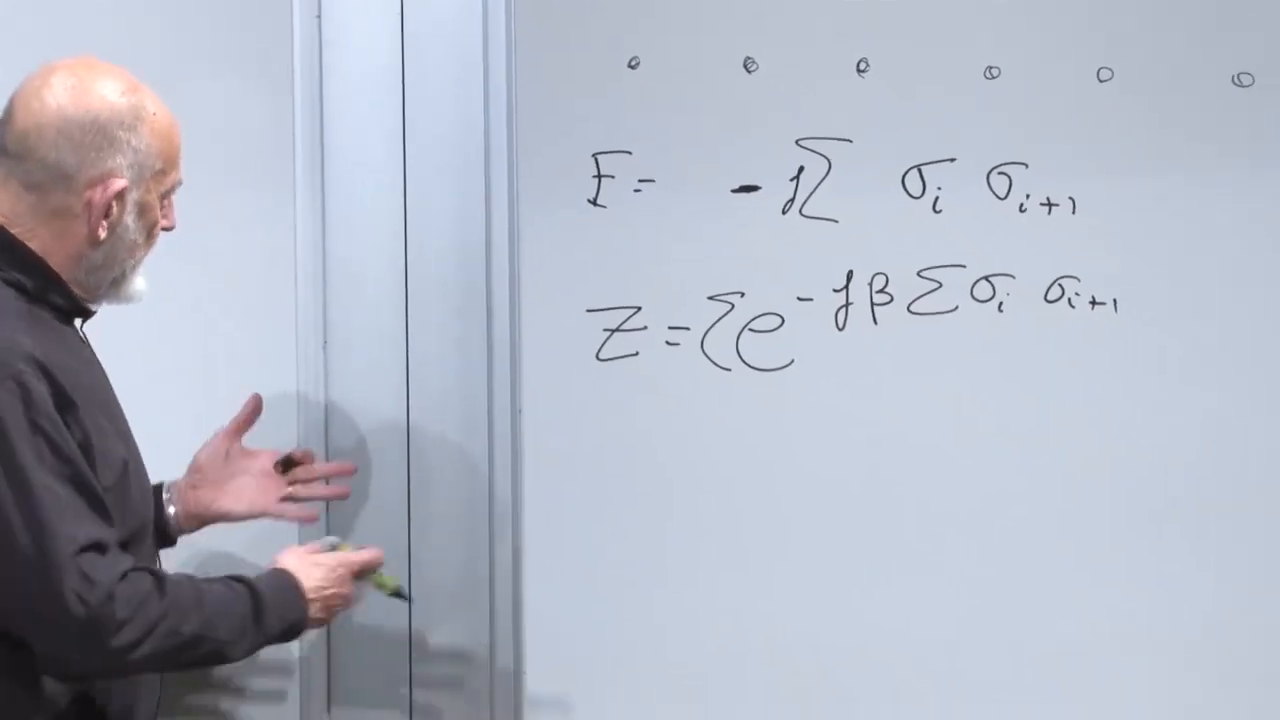
\includegraphics[width=0.80\textwidth]{lecture_09_figure_03.png}
\caption{開いた鎖のハミルトニアンとそのボルツマン和。}
\lectureframe{00:19:15}
\end{figure}

\(J\)を\(-J\)に変えると、交互に並ぶスピンが有利になる。開いた鎖、または偶数個の周期的鎖では、再定義
\begin{equation}
\widetilde{\sigma}_i=(-1)^i\sigma_i
\end{equation}
により反強磁性的な符号が強磁性的な符号に戻る。この区別は物理的であるが、一次元の分配関数の代数は同じである。奇数個の周期的鎖は、フラストレーションなしには交互に並べないため、よく知られた例外である。

\begin{classroomqa}
\audiencequestion{鎖のハミルトニアンに外部磁場はあるか？}
\lecturerresponse{まだない。式~\eqref{eq:ising-chain}には最近接結合のみが含まれている。一様な外部場は後に別の項\(-h\sum_i\sigma_i\)として加えられる。まさに、秩序状態が任意に小さなバイアスにどう応答するかを調べるためである。\lecturetimestamp{00:18:54--00:19:13}}
\end{classroomqa}

\subsection{相関関数としての記憶}

\(\sigma_i\)が上を向いていると分かっているとする。その情報は\(r\)個の結合を隔てたスピンに影響を及ぼすだろうか。診断法は
\begin{equation}
C(r)=\expect{\sigma_i\sigma_{i+r}}.
\end{equation}
である。\(C(r)\)が\(r\to\infty\)として非零の値に近づくなら、系は長距離の記憶を保持している。零に近づくなら、最初のスピンの効果はやがて消える。

伝言ゲームが正しい直観を与える。各人は次の人へ一つの二値記号を伝える。すべての伝達が完全なら、最初のビットはいつまでも生き残る。各段階にどんな非零の誤り確率があっても、伝達を繰り返すうちに元のメッセージはやがて失われる。零温度はイジング鎖の完全伝達の極限である。どんな正の温度でも、隣り合うスピンの間に時折の不一致が許される。

数値的な描像として、一回の伝達の忠実度が\(0.99\)であるとしよう。二回の完全な伝達は確率\(0.99^2=0.9801\)で起こり、段階が一つ増えるごとにさらに\(0.99\)の因子が掛かる。百段階では誤りはすでにありふれたものになり、一万段階では実用的な記憶は消える。イジング鎖はこの無誤り確率ではなく符号付きの忠実度の測度を用いるが、乗法的な損失は同じ考え方である。

この類推は、確率と相関を区別した後に厳密になる。\(p\)が隣り合うスピンが一致する確率なら、
\begin{equation}
\expect{\sigma_i\sigma_{i+1}}
=p-(1-p)=2p-1.
\end{equation}
である。したがって、結合から結合へと掛け合わされる量は過剰忠実度\(2p-1\)であり、\(p\)そのものではない。

\section{結合変数と厳密な分配関数}

決定的な変数変換は、個々のスピンではなく関係を記述することである。
\begin{equation}
\mu_i=\sigma_i\sigma_{i+1},
\qquad i=1,\ldots,N-1.
\label{eq:bond-variable}
\end{equation}
各結合変数は一致に対して\(+1\)、不一致に対して\(-1\)である。最初のスピンを固定すれば、結合がそれ以降のすべてのスピンを決める。
\begin{align}
\sigma_2&=\sigma_1\mu_1,\\
\sigma_3&=\sigma_1\mu_1\mu_2,\\
\sigma_{r+1}&=\sigma_1\prod_{k=1}^{r}\mu_k.
\end{align}
冗長性はない。データ\((\sigma_1,\mu_1,\ldots,\mu_{N-1})\)は\((\sigma_1,\ldots,\sigma_N)\)と等価である。

これらの変数ではエネルギーは単に
\begin{equation}
H=-J\sum_{i=1}^{N-1}\mu_i.
\end{equation}
である。相互作用するサイト変数は独立な結合変数になった。まず\(\sigma_1\)の二つの値について和をとると
\begin{align}
Z_N
&=2\sum_{\{\mu_i=\pm1\}}
\exp\left(\beta J\sum_{i=1}^{N-1}\mu_i\right)\\
&=2\prod_{i=1}^{N-1}
\left(\sum_{\mu_i=\pm1}e^{\beta J\mu_i}\right)\\
&=2\left[2\cosh(\beta J)\right]^{N-1}.
\label{eq:chain-partition}
\end{align}
が得られる。\(N-1\)個の因子があるのは、\(N\)個のサイトからなる開いた鎖が\(N-1\)個の結合をもつからである。

先頭の因子2は最初のスピンの大域的な選択である。それは\(\log Z_N\)に\(\log2\)だけ寄与し、一方、結合は\(N-1\)に比例する項を寄与する。この因子は厳密な有限サイズの数え上げには重要だが、\(N\to\infty\)として自由エネルギー密度からは消える。だからこそ板書はそれを実際に捨てることなく「大したことではない」と呼べたのである。

\begin{figure}[ht]
\centering
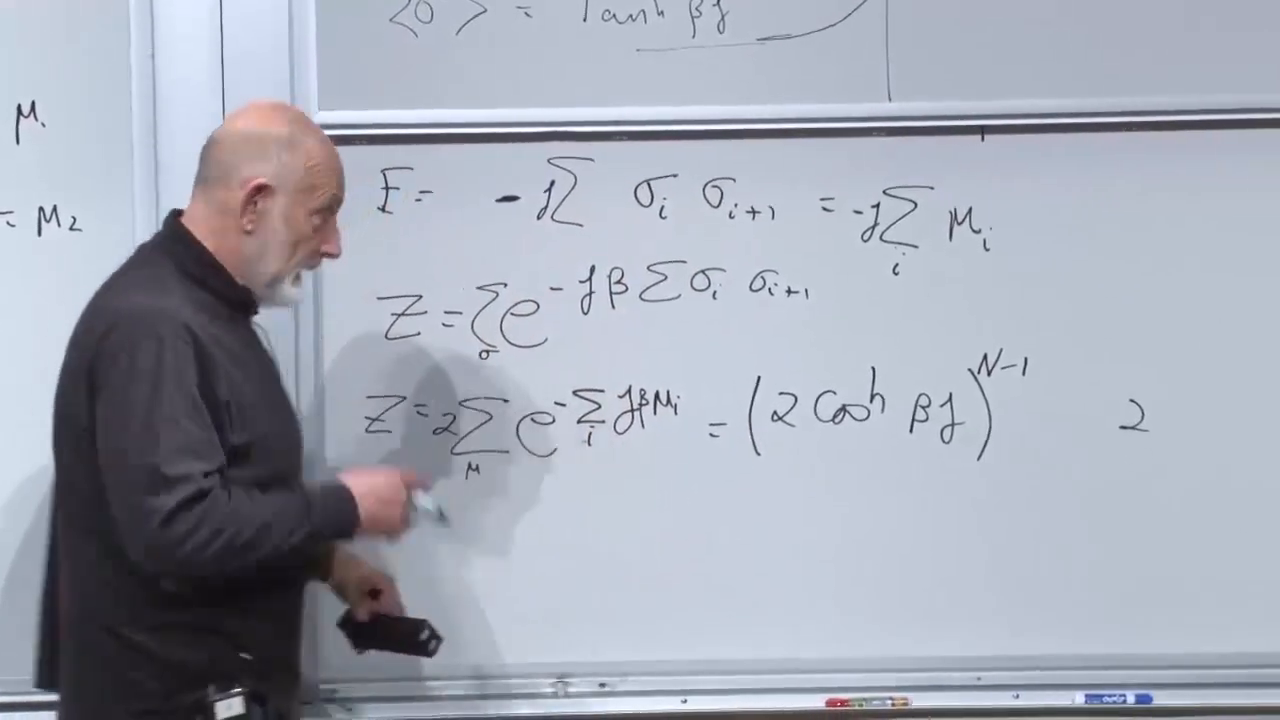
\includegraphics[width=0.82\textwidth]{lecture_09_figure_04.png}
\caption{独立な結合の和として書き直されたサイトのハミルトニアンと、その結果として因数分解された分配関数。}
\lectureframe{00:35:35}
\end{figure}

\begin{classroomqa}
\audiencequestion{最終的な答えが冪になったとき、指数の中の和はどこへ行ったのですか。}
\lecturerresponse{それは冪になる前に積になった。
\[
e^{\beta J\sum_i\mu_i}=\prod_i e^{\beta J\mu_i}.
\]
すべての結合配置にわたる和は、各結合に対する一つの二項の和に分離する。すべての因子が\(2\cosh(\beta J)\)であるから、積はその\((N-1)\)乗である。三つのスピンと二つの結合を書き下せば、因数分解は完全に明示的になる。\lecturetimestamp{00:33:25--00:35:36}}
\end{classroomqa}

これは単純な双対記述である。サイト上の結合した変数が、結合上の結合していない変数に置き換えられた。\emph{双対性}という語が適切なのは、同じ系が非常に異なって見える自由度をもつ二つの記述をもつからである。ここではそれは開いた一次元鎖に対する厳密な変数変換である。

格子の言葉では、元の変数は頂点に住み、新しい変数は辺に住む。最初のスピンの大域的な選択は、辺から頂点を再構成するために必要な唯一の余分なデータである。このサイトと結合の交換は、より高次元の統計力学ではるかに強力になるパターンのささやかな例である。

\subsection{最近接忠実度}

すべての結合は同じ分布をもち、
\begin{equation}
\begin{aligned}
\Pr(\mu=+1)&=\frac{e^{\beta J}}{2\cosh(\beta J)},\\
\Pr(\mu=-1)&=\frac{e^{-\beta J}}{2\cosh(\beta J)}.
\end{aligned}
\end{equation}
である。したがって、
\begin{equation}
\expect{\mu_i}
=\expect{\sigma_i\sigma_{i+1}}
=\tanh(\beta J).
\label{eq:nearest-correlation}
\end{equation}

\begin{figure}[ht]
\centering
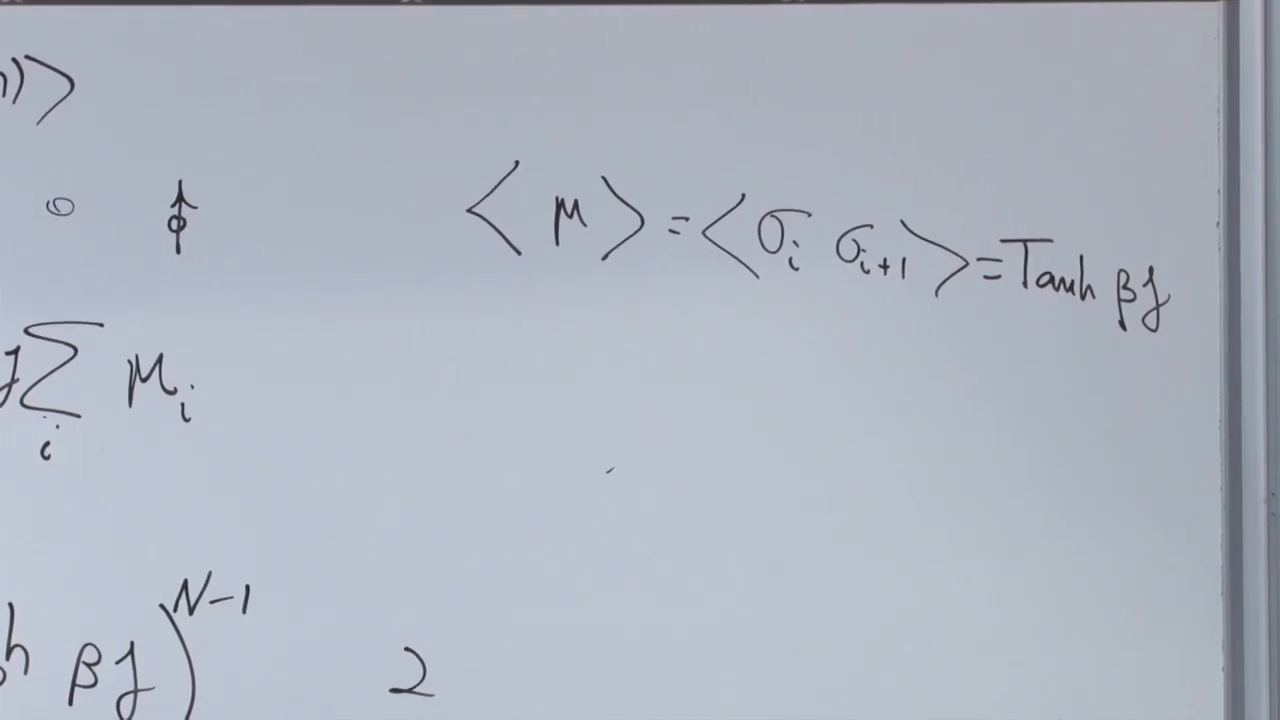
\includegraphics[width=0.80\textwidth]{lecture_09_figure_05.png}
\caption{平均結合変数として表された最近接相関。}
\lectureframe{00:36:52}
\end{figure}

したがって、隣り合うスピンが一致する確率は
\begin{equation}
p_{\rm same}
=\frac{1+\tanh(\beta J)}{2}.
\end{equation}
である。これは正の\(J\)で二分の一を超え、零温度で一に近づき、無限温度で二分の一になる。

\begin{classroomqa}
\audiencequestion{なぜ正の最近接相関は、スピンが反平行よりも平行を好むことを意味するのか。}
\lecturerresponse{\(J>0\)では、平行な結合のエネルギーは\(-J\)であり、反平行な結合のエネルギーは\(+J\)である。\(\expect{\mu}\)が正であることは、\(\mu=+1\)、すなわち平行がより頻繁に起こることを示している。実際の物質が強磁性または反強磁性の有効結合をもつかどうかは、その微視的な電子構造に依存する。ここでの符号の規約は強磁性体を記述している。\lecturetimestamp{00:43:45--00:44:48}}
\end{classroomqa}

\begin{classroomqa}
\audiencequestion{非常に高温ではこの相関はどうなるか。}
\lecturerresponse{\(T\to\infty\)のとき、\(\beta\to0\)かつ\(\tanh(\beta J)\to0\)となる。すると最近接のスピン同士でさえ互いについて何の情報ももたない。各スピンは実質的にランダムな推測である。\lecturetimestamp{00:46:42--00:47:20}}
\end{classroomqa}

\subsection{長距離相関}

\(r\)本だけ離れたスピンに対して、
\begin{align}
\sigma_i\sigma_{i+r}
&=\sigma_i
\left(\prod_{k=i+1}^{i+r-1}\sigma_k^2\right)
\sigma_{i+r}\\
&=(\sigma_i\sigma_{i+1})
(\sigma_{i+1}\sigma_{i+2})\cdots
(\sigma_{i+r-1}\sigma_{i+r})\\
&=\prod_{k=i}^{i+r-1}\mu_k.
\end{align}
\(\mu_k\)は独立であるから、
\begin{equation}
C(r)=\expect{\sigma_i\sigma_{i+r}}
=\left[\tanh(\beta J)\right]^r.
\label{eq:exact-correlation}
\end{equation}

\begin{figure}[ht]
\centering
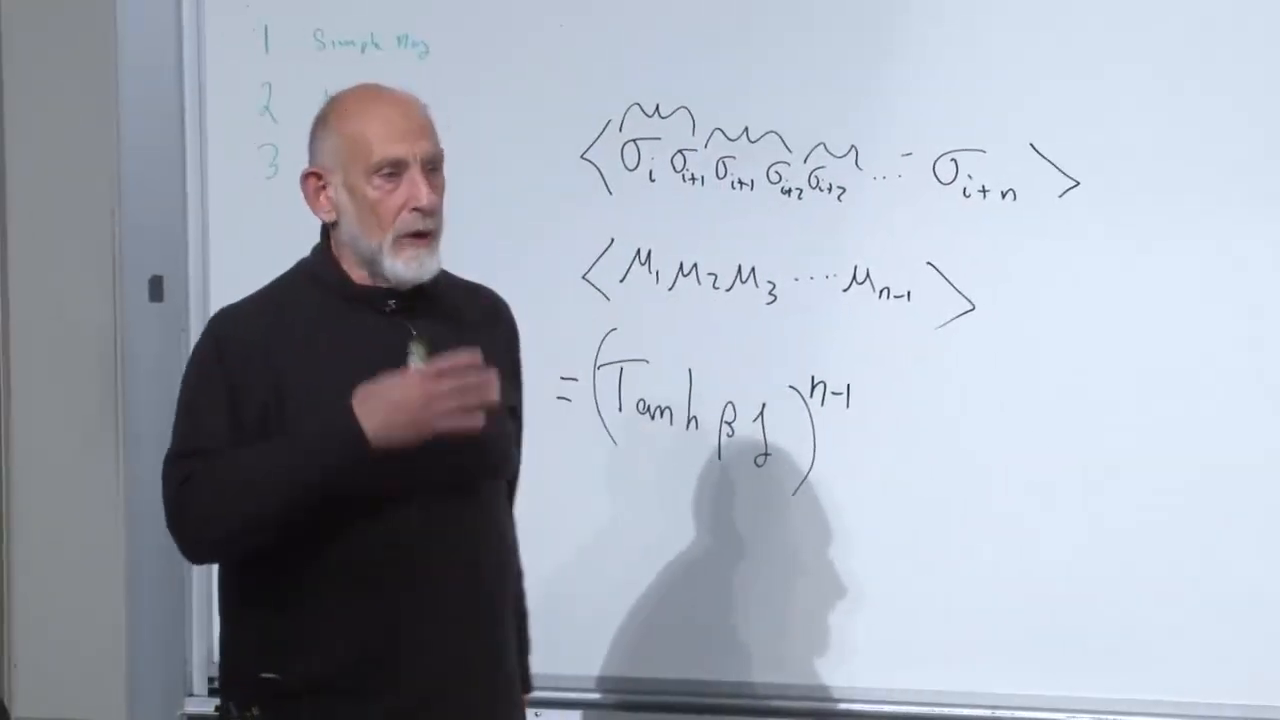
\includegraphics[width=0.80\textwidth]{lecture_09_figure_06.png}
\caption{中間の\(\sigma_k^2=1\)の因子が、遠方のスピンの積を独立な結合の積に変換する。}
\lectureframe{00:41:35}
\end{figure}

\begin{classroomqa}
\audiencequestion{相関関数には両端のスピンしか含まれていない。中間のスピンはどこから来たのか。}
\lecturerresponse{それらは1の因子として挿入されただけである: \(\sigma_k^2=1\)。隣接するコピーを対にすることで、端点の積が結合変数に変換される。結合変数こそ、その熱分布が因子分解する変数である。相関関数の値は変わっていない。\lecturetimestamp{00:41:41--00:42:26}}
\end{classroomqa}

すべての有限温度で、
\begin{equation}
0<\tanh(\beta J)<1,
\end{equation}
であるから、記憶は指数関数的に減衰する。
\begin{equation}
C(r)=e^{-r/\xi}
\end{equation}
と書くと、厳密な相関長
\begin{equation}
\xi^{-1}=-\log\!\left[\tanh(\beta J)\right].
\label{eq:correlation-length}
\end{equation}
が定義される。\(T=0\)においてのみ\(\xi\)は発散する。低いがゼロでない温度では、
\begin{equation}
\xi\simeq \frac{1}{2}e^{2\beta J},
\end{equation}
であるから、鎖は真の無限距離秩序をもつことなく、非常に長い平行な連なりを含むことができる。

したがって鎖は塊状に見える。上向きスピンの長い連なりがあり、次に切り替わり、下向きスピンの長い連なりがあり、さらに別の切り替わりがある。低温は、ドメイン壁が稀であるために連なりを長くするが、ドメイン壁を完全に排除するわけではない。磁化には、単に非常に大きいだけでなく、無限の記憶長が必要である。

\section{隣人が増えると問題がどう変わるか}

1次元では誤り訂正ができない。ある結合がその前の結合と一致しなくなると、次のスピンには、どちらの向きが意図されていたかを独立に告げる情報源がない。したがって鎖は、時折の切り替わりで隔てられた長い平行ドメインからなる。

正方格子では各サイトは4つの最近接サイトをもつ。立方格子では6つである。\(d\)次元超立方格子では、
\begin{equation}
z=2d
\end{equation}
個の最近接サイトをもつ。3つの一致するメッセージと1つの不一致メッセージを受け取るサイトは多数決に従うことができる。多数の隣人の環境は、冗長なメッセージが誤り訂正を可能にするのとほぼ同じ仕方で、孤立した誤りを抑圧する。

隣人が平均スピン\(m\)をもつなら、その和の平均は\(zm\)である。その通常の揺らぎは\(\sqrt{z}\)の程度であるから、\(m=0\)から離れると、相対揺らぎはおよそ
\begin{equation}
\frac{\sqrt{z}}{z|m|}
=\frac{1}{\sqrt{z}\,|m|}.
\end{equation}
とスケールする。これが、大きな配位数で平均場がもっともらしくなる理由である。また、\(m\)が小さい臨界点の近くで近似が最も信頼できなくなることも警告している。

記憶に残る格言が大数の直観を捉えている。100の独立な投票が同じ方向に誤ることは unlikely である。定量的な版は平方根則である。\(z\)個の変数におけるコヒーレントなバイアスは\(z\)に比例するが、ランダムな不一致は通常\(\sqrt{z}\)にしか比例しない。したがって次元を増やすことは、隣人の数だけでなく、その集団的メッセージの信頼性をも変える。

\begin{classroomqa}
\audiencequestion{3より高い次元は物理的な磁性体に対応するのか。}
\lecturerresponse{空間次元として直接対応するわけではない。大きな\(d\)は、各サイトが多くの隣人をもち、平均化が制御可能になる可解極限である。そこで機構が見えれば、それが物理的な次元にどこまで生き残るかを問うことができる。イジング模型では、平均場は厳密な2次元の答えを与えないが、2次元ですでに有限温度転移には十分である。\lecturetimestamp{00:52:32--00:53:50}}
\end{classroomqa}

\section{自己無撞着問題としての平均場}

一つのスピン\(\sigma_i\)に注目する。その\(z=2d\)個の最近接スピンとの相互作用は
\begin{equation}
E_i=-J\sigma_i\sum_{j\in{\rm nn}(i)}\sigma_j.
\label{eq:local-energy}
\end{equation}
である。
\begin{equation}
m=\expect{\sigma}
\end{equation}
をスピン当たりの一様磁化とする。平均場近似では、揺らぐ最近接スピンの和をその平均で置き換える：
\begin{equation}
\sum_{j\in{\rm nn}(i)}\sigma_j
\longrightarrow zm=2dm.
\end{equation}
このとき、注目したスピンの有効一スピンエネルギーは
\begin{equation}
E_i^{\rm MF}=-2dJm\,\sigma_i.
\label{eq:mean-field-energy}
\end{equation}
となる。

\begin{figure}[ht]
\centering
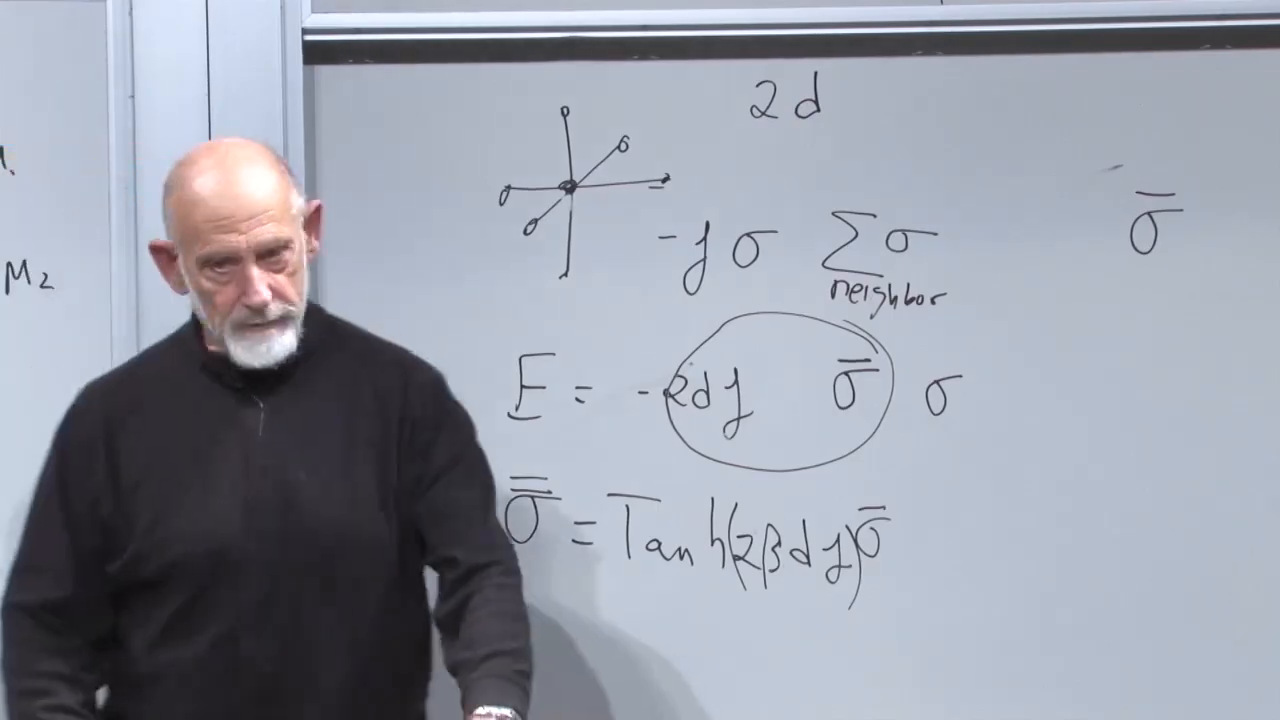
\includegraphics[width=0.82\textwidth]{lecture_09_figure_07.png}
\caption{選ばれたスピン、その\(2d\)個の最近接スピン、およびそれらの和を平均磁化で置き換えること。}
\lectureframe{01:00:30}
\end{figure}

一スピンの結果は、有効場\(2dJm\)を用いて再利用できる：
\begin{equation}
\expect{\sigma_i}_{\rm effective}
=\tanh(2\beta dJm).
\end{equation}
しかし、選ばれたサイトは特別ではない。並進不変性により、その平均は仮定された平均\(m\)に等しくなければならない。したがって
\begin{equation}
\boxed{m=\tanh(2\beta dJm)}.
\label{eq:self-consistency}
\end{equation}
これが、平均場が自己無撞着場近似とも呼ばれる理由である：有効場を生み出す磁化は、その場によって生み出される磁化に等しくなければならない。

\begin{classroomqa}
\audiencequestion{有効一スピンの答えには\(\beta\)の因子が欠けているのか？}
\lecturerresponse{それは存在しなければならない。指数関数や双曲線正接の引数は無次元であるから、有効エネルギー\(2dJm\)は\(2\beta dJm\)として現れる。\lecturetimestamp{01:00:13--01:00:27}}
\end{classroomqa}

\begin{classroomqa}
\audiencequestion{この方程式は、\(m\)がそれ自身に比例すると述べているだけなのか？}
\lecturerresponse{いいえ。未知の磁化は非線形関数の内部に現れる：
\[
m=\tanh(2\beta dJm).
\]
これは陰方程式であり、温度に応じて一つまたは複数の解を持ちうる。\lecturetimestamp{01:02:12--01:02:42}}
\end{classroomqa}

\begin{classroomqa}
\audiencequestion{自己無撞着方程式は、高温または双曲線正接の小さな引数を仮定しているのか？}
\lecturerresponse{いいえ。方程式\(m=\tanh(2\beta dJm)\)は、すべての温度における完全な平均場方程式である。\(\tanh x\simeq x\)のような後の近似のみが小さな\(x\)を必要とし、それは臨界点近傍で、現れる解を特定したり展開したりするために用いられる。\lecturetimestamp{01:02:44--01:03:12}}
\end{classroomqa}

\begin{classroomqa}
\audiencequestion{上線の記法は、通常の山括弧による平均とは異なるのか？}
\lecturerresponse{いいえ。黒板で用いられるバーは、熱平均の略記である：\(\bar{\sigma}=\expect{\sigma}=m\)。\lecturetimestamp{01:03:19--01:03:42}}
\end{classroomqa}

\begin{classroomqa}
\audiencequestion{\(2d\)個のスピンはすべて最近接スピンなのか、またより長距離の結合も同様の効果を持つのか？}
\lecturerresponse{超立方格子上では、はい：\(d\)個の座標軸のそれぞれに沿って二つの最近接スピンが存在する。次近接およびより遠い結合は別の模型であり、一般にそれぞれ独自の強さを持つが、相互作用の範囲を広げることは有効配位数も増やし、平均場の推論をより正確にしうる。\lecturetimestamp{01:03:43--01:05:12}}
\end{classroomqa}

\section{相転移のグラフ化}

定義する
\begin{equation}
K=2\beta dJ,
\qquad
y=Km.
\end{equation}
すると式~\eqref{eq:self-consistency}は
\begin{equation}
\frac{y}{K}=\tanh y.
\label{eq:graph-equation}
\end{equation}
となる。右辺は固定されたシグモイドである。左辺は原点を通る傾き
\begin{equation}
\frac{1}{K}=\frac{T}{2dJ},
\end{equation}
の直線である。ここで\(k_{\rm B}=1\)。

高温では直線は急であり、\(\tanh y\)と\(y=0\)のみで交わる。低温では直線は緩やかであり、三つの交点が存在する：\(y=0\)および対称な対\(y=\pm y_0\)。閾値は、直線と\(\tanh y\)が原点で同じ傾きを持つときに生じる。\(\tanh'(0)=1\)であるから、
\begin{equation}
K_c=1,
\qquad
T_c^{\rm MF}=2dJ.
\label{eq:mean-field-tc}
\end{equation}
これが平均場臨界温度であり、低次元における厳密な答えではない。

仮定\(J>0\)は、隣接スピンが一致することを好むと言っている；それは\(+m\)を\(-m\)より選び出すものではない。外部場がゼロのとき、ハミルトニアンは大域的フリップ\(\sigma_i\mapsto-\sigma_i\)によって変わらないので、二つの非零交点は物理的に等価である。グラフの正の半分のみを選ぶことは便利な作図上の慣習であり、負の相を失うことではない。

\begin{figure}[ht]
\centering
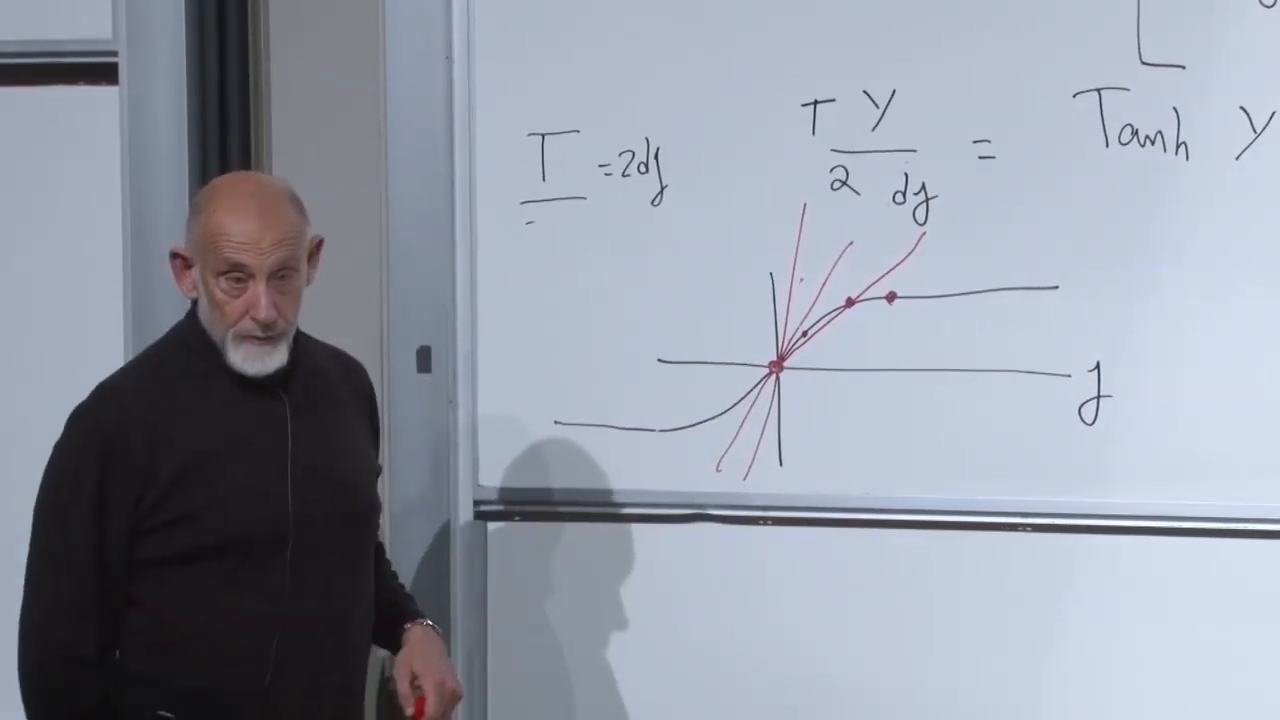
\includegraphics[width=0.82\textwidth]{lecture_09_figure_08.png}
\caption{直線族と\(\tanh y\)：高温での単一交点と低温での三つの交点。}
\lectureframe{01:11:50}
\end{figure}

\begin{figure}[ht]
\centering
\begin{tikzpicture}[x=1.15cm,y=2.0cm]
\draw[->] (-3.2,0) -- (3.2,0) node[right] {$y$};
\draw[->] (0,-1.15) -- (0,1.15);
\draw[thick,blue!70!black,domain=-3:3,samples=120]
  plot (\x,{tanh(\x)}) node[right] {$\tanh y$};
\draw[thick,red!70!black] (-0.85,-1.15) -- (0.85,1.15)
  node[pos=0.70,left] {high \(T\)};
\draw[thick,orange!85!black] (-1.15,-1.15) -- (1.15,1.15)
  node[pos=0.86,right] {\(T_c^{\rm MF}\)};
\draw[thick,green!45!black] (-3,-0.72) -- (3,0.72)
  node[right] {low \(T\)};
\fill (0,0) circle (1.4pt);
\fill[green!45!black] (-2.45,-0.588) circle (1.5pt);
\fill[green!45!black] (2.45,0.588) circle (1.5pt);
\end{tikzpicture}
\caption{図形的自己無撞着論法の正規化された再構成。}
\end{figure}

非零の枝は連続的に現れる。転移近傍では、
\begin{equation}
\tanh(Km)=Km-\frac{(Km)^3}{3}+O(m^5).
\end{equation}
\(K>1\)に対して、小さな非零解は
\begin{equation}
m^2\simeq \frac{3(K-1)}{K^3}.
\end{equation}
を満たす。したがって平均場は、よく知られた平方根の立ち上がり\(m\propto(T_c-T)^{1/2}\)を予言する。

安定性の記述は、グラフがどのように描かれるかに依拠せずに行うこともできる。\(m\)に依存しない定数を除いて、一スピンあたりの平均場自由エネルギーは
\begin{equation}
f_{\rm MF}(m)
=dJm^2-\frac{1}{\beta}
\log\!\left[2\cosh(2\beta dJm)\right].
\label{eq:mf-free-energy}
\end{equation}
である。その停留条件は
\begin{equation}
\frac{\partial f_{\rm MF}}{\partial m}
=2dJ\left[m-\tanh(2\beta dJm)\right]=0.
\end{equation}
である。\(T_c^{\rm MF}\)より上では、\(m=0\)が最小である。それより下では、原点は局所的最大であり、二つの非零解は縮退した最小である。交点の幾何学と自由エネルギーの熱力学は同じことを述べている。

\begin{classroomqa}
\audiencequestion{解\(m=0\)は\(T_c^{\rm MF}\)の下で依然として交点である。なぜ非零の分枝が物理的でなければならないのか。}
\lecturerresponse{系を零温度から上昇させていくと、すでに磁化した分枝上に置かれる。より形式的には、平均場自由エネルギーは転移点以下で\(\pm m_0\)に極小をもち、一方\(m=0\)は極大となる。そのとき無限小の外部場が一方の極小を選び、見かけの曖昧さを取り除く。\lecturetimestamp{01:11:34--01:12:18}}
\end{classroomqa}

\section{なぜ一次元では平均場が破れるのか}

\(d=1\)を式~\eqref{eq:mean-field-tc}に代入すると、\(T=2J\)に転移があると予言することになり、厳密な一次元解と矛盾する。代数的に発散するものは何もない。この近似が破れるのは、二つの隣接スピンが大きな統計的浴ではないからであり、また一次元のドメイン壁が例外的なエントロピーを担うからである。

すべて上向きの状態から始める。壊れた結合はそのエネルギーを\(-J\)から\(+J\)へ変えるので、壊れた結合一つあたりのコストは
\begin{equation}
\Delta E_{\rm bond}=2J.
\end{equation}
である。正方格子上では、反転したスピン一つが四つの結合を壊し、\(8J\)のコストがかかる。隣接する反転スピン二つは六つの壊れた結合からなる周囲長をもち、\(12J\)のコストがかかるのに対し、遠く離れた反転二つは八つの結合を壊し、\(16J\)のコストがかかる。

\begin{figure}[ht]
\centering
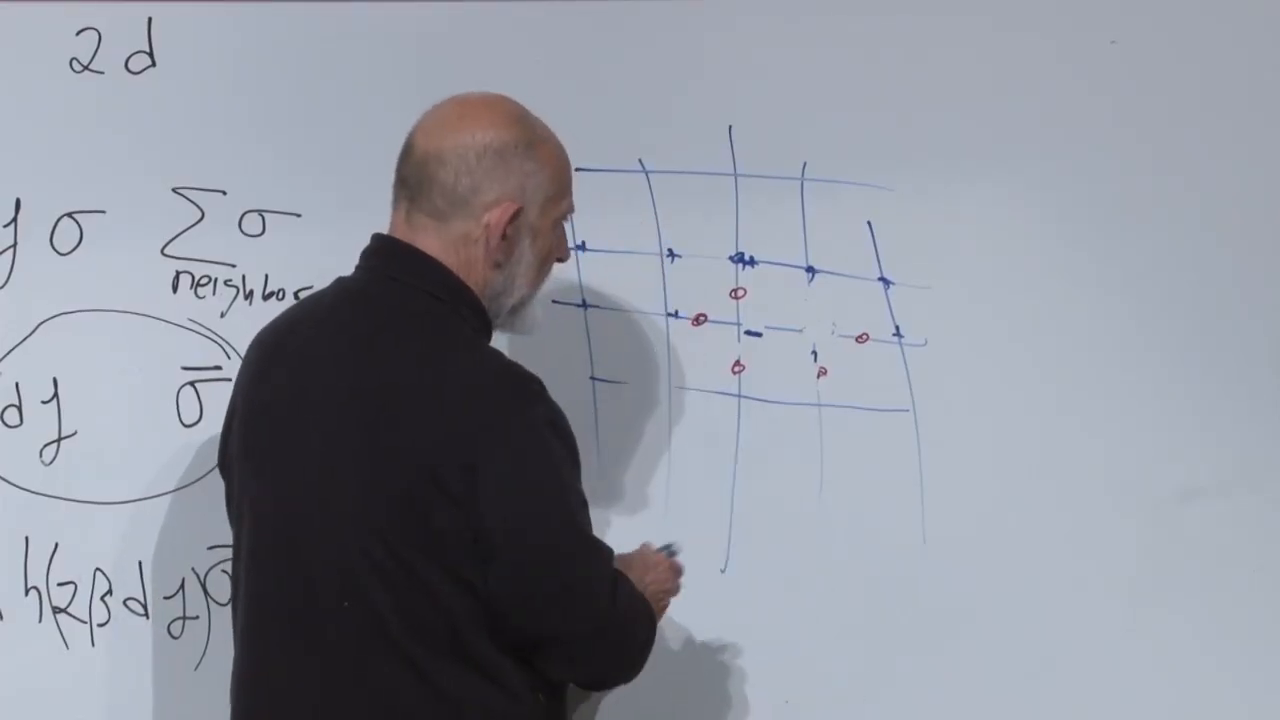
\includegraphics[width=0.82\textwidth]{lecture_09_figure_09.png}
\caption{正方格子上の隣接する反転スピン二つ。それらの共有結合は満たされており、六結合の境界が残る。}
\lectureframe{01:17:30}
\end{figure}

したがって二次元では、コンパクトな反転液滴はその境界長に比例するエネルギーを支払う：
\begin{equation}
\Delta E_{\rm 2d}=2J\,|\partial D|.
\end{equation}
液滴を成長させると、一般にその境界も成長する。

一次元は異なる。連続した反転ブロックは、どれほど長くても二つのドメイン壁しかもたない：
\begin{equation}
\Delta E_{\rm 1d}=2(2J)=4J.
\label{eq:one-d-domain-cost}
\end{equation}

\begin{figure}[ht]
\centering
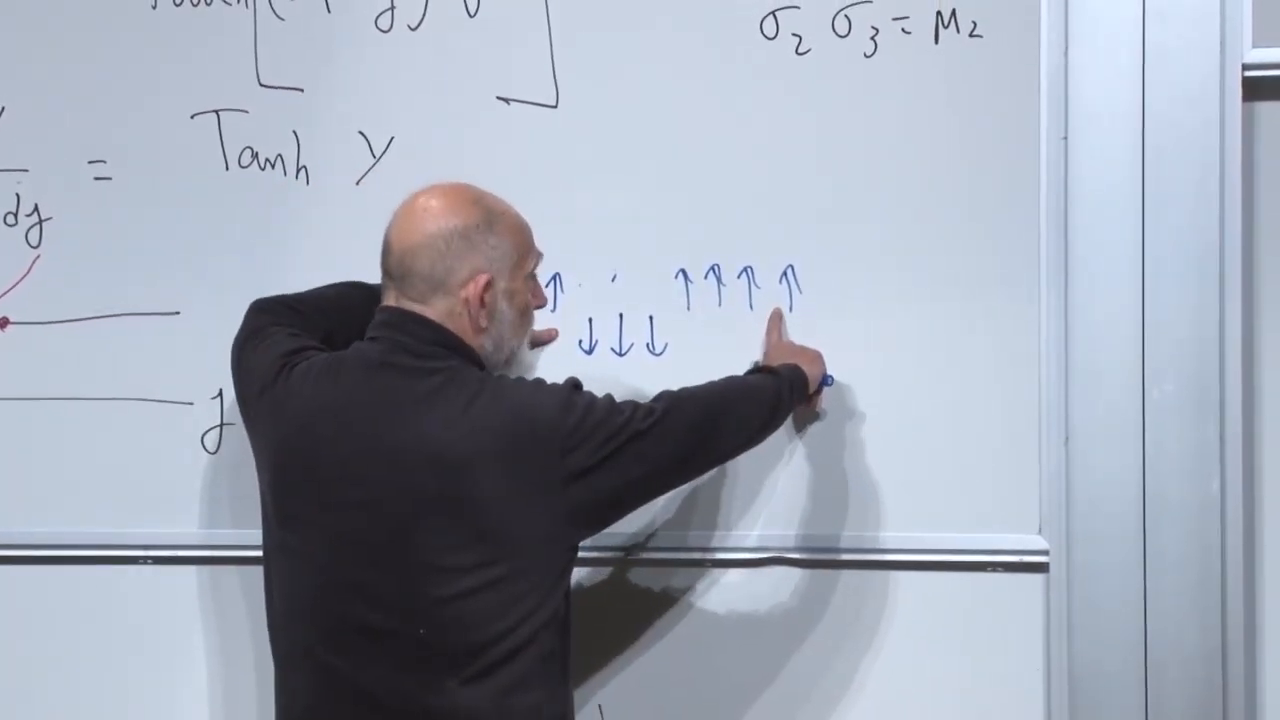
\includegraphics[width=0.82\textwidth]{lecture_09_figure_10.png}
\caption{一次元における長い反転ブロックは、二つのドメイン壁だけに囲まれている。}
\lectureframe{01:19:10}
\end{figure}

\(N\)サイトの鎖において、そのようなブロックの二つの壁を選ぶ方法は\(N^2\)の程度ある。それらのエネルギーは壁間の間隔とともに成長しない。任意の正の温度で、したがってエントロピーは任意に大きな反転ドメインを供給する。二次元では、境界エネルギーは十分低い温度で輪郭のエントロピーを打ち負かすことができる。このエネルギーとエントロピーの競合は、\(d=1\)と\(d=2\)を同じ係数の異なる数値として扱うとき、平均場が見ることのできない幾何学的事実である。

\begin{classroomqa}
\audiencequestion{二つの壁の一定コストは、反転スピンが隣接していることを要求するのか。}
\lecturerresponse{はい。この主張は一つの連続した反転ブロックに関するものである。反転スピンがいくつかの分離したブロックを形成するなら、各ブロックは二つの追加のドメイン壁を導入する。重要な点は、単一のブロックが二つの壁だけを保ちながら任意に長くなりうることである。\lecturetimestamp{01:18:32--01:18:40}}
\end{classroomqa}

\begin{classroomqa}
\audiencequestion{平均場方程式自体は\(d=1\)と\(d=2\)の間に定性的な区別を示さないように見える。それが問題なのか。}
\lecturerresponse{まさにその通りである。平均場はすべての正の\(d\)に対して転移を予言するので、一次元では定性的に誤っている。その導出は多数の弱く揺らぐ隣接スピンを仮定し、ドメイン壁の幾何学を捨て去った。一次元の場合を決めるのは、平均場の代入\(d=1\)ではなく、厳密な結合解である。\lecturetimestamp{01:19:44--01:20:28}}
\end{classroomqa}

\section{外部場が相を選ぶ}

\(h>0\)が\(\sigma=+1\)を好むという規約で、一様な場\(h\)を加える：
\begin{equation}
H=-J\sum_{\langle ij\rangle}\sigma_i\sigma_j
-h\sum_i\sigma_i.
\label{eq:ising-with-field}
\end{equation}
選ばれた一つのスピンの平均場エネルギーは
\begin{equation}
E_i^{\rm MF}=-(2dJm+h)\sigma_i,
\end{equation}
であり、自己無撞着方程式は
\begin{equation}
\boxed{m=\tanh\!\left[\beta(2dJm+h)\right]}.
\label{eq:self-consistency-field}
\end{equation}
となる。\(K=2\beta dJ\)および\(y=Km\)とすると、
\begin{equation}
\frac{y}{K}=\tanh(y+\beta h).
\label{eq:shifted-graph}
\end{equation}

\begin{figure}[ht]
\centering
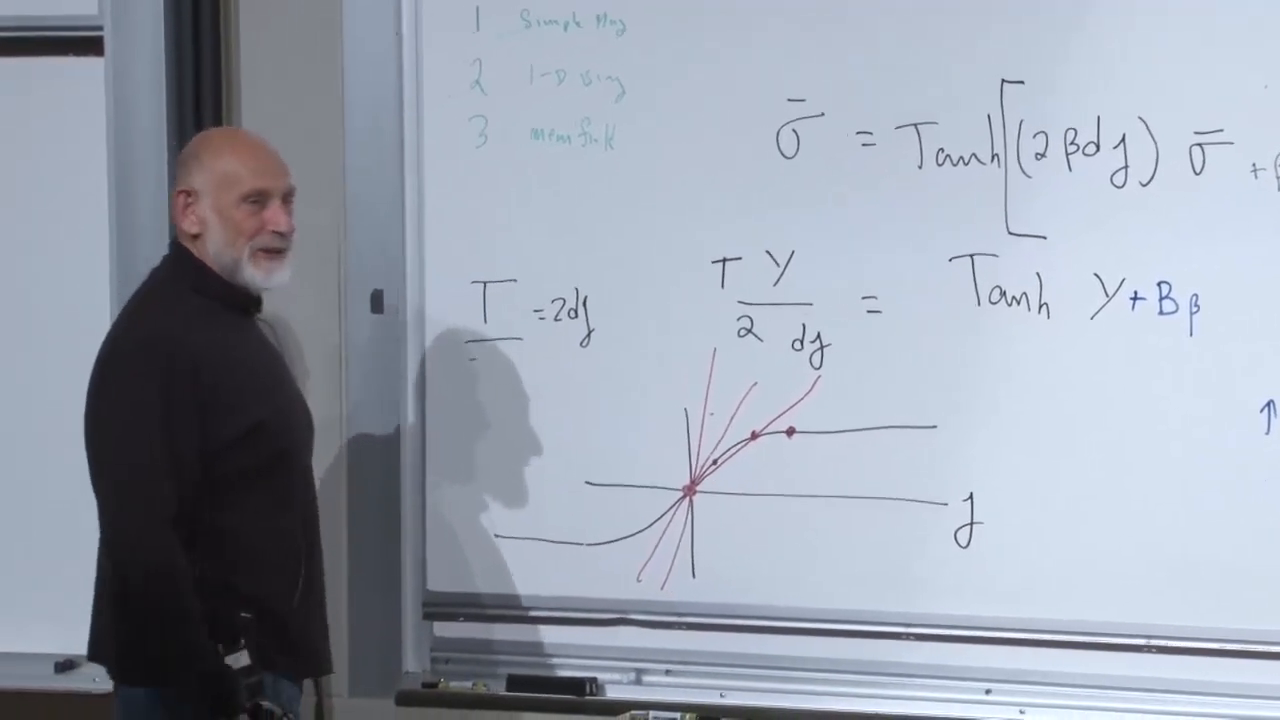
\includegraphics[width=0.82\textwidth]{lecture_09_figure_11.png}
\caption{自己無撞着方程式に加えられた外部場の項と、それに対応する平行移動した図式構成。}
\lectureframe{01:26:20}
\end{figure}

\begin{classroomqa}
\audiencequestion{なぜ場は双曲線正接の内部にのみ加えられるのか。左辺も変えるべきではないのか。}
\lecturerresponse{左辺は仮定された磁化\(m\)、あるいは同等に\(y/K\)である。右辺は全有効場\(2dJm+h\)中のスピンに対して計算された磁化である。自己無撞着性はそれら二つの量を等しく置く。\(y=Km\)を定義として固定しておくと、新しい項は引数\(\tanh(y+\beta h)\)の中にのみ入る。\lecturetimestamp{01:23:46--01:26:18}}
\end{classroomqa}

\begin{classroomqa}
\audiencequestion{同じ図式的変化は、\(\tanh\)曲線をずらすのではなく直線を動かすことによって記述できるか。}
\lecturerresponse{はい。\(\tanh y\)を固定したまま、直線が非零の切片をもつように方程式を書き直せばよい。交点は同一である。二つの記述は、方程式のどちら側を固定されたグラフとして選ぶかだけが異なる。\lecturetimestamp{01:35:07--01:36:26}}
\end{classroomqa}

\(h\neq0\)では、もはや原点は解ではない。\(T_c^{\rm MF}\)より下では、任意に小さい正の磁場が正の枝を選び、負の磁場が負の枝を選ぶ。

\begin{figure}[ht]
\centering
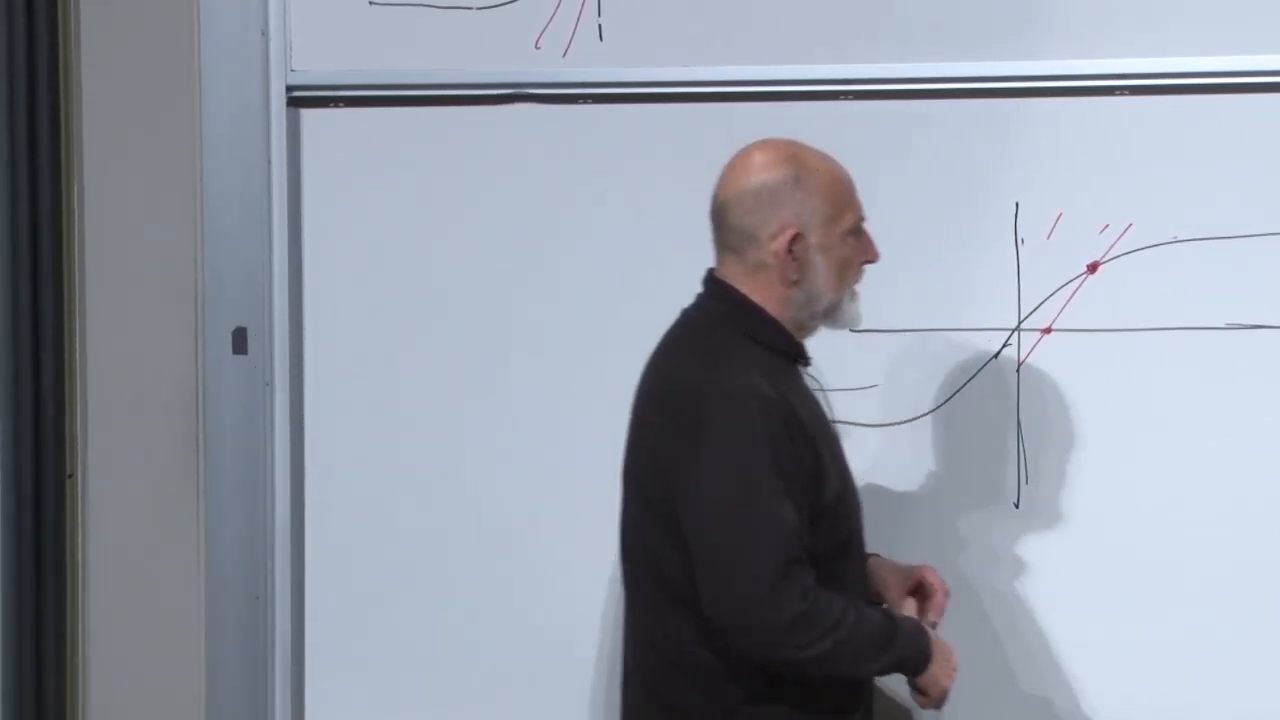
\includegraphics[width=0.82\textwidth]{lecture_09_figure_12.png}
\caption{弱い磁場は対称な交点を取り除き、磁化した一方の枝を選ぶ。}
\lectureframe{01:36:22}
\end{figure}

正確な記述には極限の順序が必要である。ちょうど\(h=0\)における有限系はスピン反転対称性をもつため、完全な平衡集団では\(\expect{m}=0\)である。自発磁化は
\begin{equation}
m_{\rm sp}
=\lim_{h\to0^+}\lim_{N\to\infty}\expect{m}_{N,h},
\end{equation}
であり、熱力学極限を先に取る。微小磁場の符号を逆にすると\(-m_{\rm sp}\)となる。全磁場エネルギーの差は\(Nh\)に比例するので、巨視的な試料ではごく小さな磁場でも決定的になる。

対応する自由エネルギーは傾きを可視化する：
\begin{equation}
f_{\rm MF}(m;h)
=dJm^2-\frac{1}{\beta}
\log\!\left[2\cosh\!\left(\beta(2dJm+h)\right)\right].
\end{equation}
\(h=0\)では二つの井戸は同じ深さである。正の\(h\)は正の\(m\)の井戸を下げ、負の\(m\)の井戸を上げる。スピン当たりの摂動はごく小さくても、\(N\)を掛けた全体的な選好は巨視的である。

\begin{classroomqa}
\audiencequestion{外部磁場が存在し続けるなら、磁化は本当に自発的なのか。}
\lecturerresponse{磁場は枝を選ぶためにのみ用いられる。\(T<T_c\)を固定し、系を無限大にしてから\(h\to0^+\)とする。選別磁場が消えても磁化は有限のままである。極限の符号を逆にすると反対の相が選ばれる。\lecturetimestamp{01:33:15--01:34:18}}
\end{classroomqa}

\begin{classroomqa}
\audiencequestion{転移より下で、平均ゼロの解は実際に不可能なのか、それとも単に不安定なだけなのか。}
\lecturerresponse{ちょうど磁場ゼロでは、二つの配向に等しい重みを与える対称な有限体積集団は可能であり、平均はゼロである。失敗するのは、単一の巨視的相としてのその安定性である。任意に小さい磁場が示量的なエネルギー均衡を変え、一方の配向を選ぶ。熱力学極限の後、選ばれた磁化は磁場を取り除いても生き残る。\lecturetimestamp{01:34:25--01:35:06}}
\end{classroomqa}

\begin{classroomqa}
\audiencequestion{無限温度で磁場に偏った解はどうなるのか。}
\lecturerresponse{固定された有限の\(h\)に対し、\(K=2\beta dJ\)と\(\beta h\)はともに\(T\to\infty\)で消える。式~\eqref{eq:self-consistency-field}はそのとき\(m\to0\)を与える。弱い磁場は低温の枝を選ぶが、無限の熱的攪乱に抗して秩序を維持することはできない。\lecturetimestamp{01:27:39--01:29:51}}
\end{classroomqa}

\begin{classroomqa}
\audiencequestion{温度とグラフのずれを同時に変えるとき、交点がどこへ行くかをどう確かめられるのか。}
\lecturerresponse{陰伏方程式は動くスケッチより安全である。低温で正の\(h\)では、その安定解は\(m=+1\)に近づく。高温では、正接の展開により
\[
m\simeq \beta(2dJm+h)
\quad\Longrightarrow\quad
m\simeq \frac{\beta h}{1-2\beta dJ},
\]
が得られ、これは\(\beta\to0\)でゼロに近づく。したがって安定枝は、整列した低温極限を弱く分極した高温極限へつなぎ、転移より下で不安定な原点にとどまることはない。\lecturetimestamp{01:29:53--01:33:04}}
\end{classroomqa}

\section{磁気反転は別の問題である}

\begin{classroomqa}
\audiencequestion{地球の磁場を反転させるものは何か。}
\lecturerresponse{その問いは平衡イジング模型の範囲外である。地球の主磁場はジオダイナモによって生成される。外核における電気伝導性流体の対流と回転が電流と磁場を維持する。反転はその非線形ダイナモの不規則な再編成であり、固体鉄における単純な強磁性ドメインの反転ではない。その詳細なタイミングは一つの平衡秩序変数では捉えられないので、ここでの正直な答えは、イジング計算は引き金を説明しないというものである。有用な関連は一般的なものに限られる。すなわち、二つの反対の大規模配向をもつ系はそれらの間で不安定性を起こしうる。\footnote{\href{https://science.nasa.gov/science-research/earth-science/earths-magnetosphere-protecting-our-planet-from-harmful-space-energy/}{ジオダイナモに関するNASAの概説}と\href{https://www.usgs.gov/programs/geomagnetism/introduction-geomagnetism}{地磁気に関するUSGSの入門}を参照。} \lecturetimestamp{01:38:39--01:40:32}}
\end{classroomqa}

厳密な鎖と平均場格子は今や二つの際立って異なる答えを与える。一次元では、
\begin{equation}
\expect{\sigma_i\sigma_{i+r}}
=\left[\tanh(\beta J)\right]^r
\longrightarrow0
\qquad (T>0),
\end{equation}
なぜなら有限エネルギーのドメイン壁が任意に長い反転区間を分離できるからである。多数の隣接スピンがある場合、自己無撞着場は代わりに
\begin{equation}
T_c^{\rm MF}=2dJ.
\end{equation}
より下で安定な非ゼロ解を許す。この対比は単に代数的なものではない。それは幾何、エネルギー、エントロピー、冗長性の間の競合である。すなわち、誤りが自由に広がりうるか、周囲の格子がそれを訂正できるかどうかである。
\chapter{イジング磁性体から液体--気体臨界現象へ}

\lectureoverview{液体--気体転移には、予想外の道筋から到達できる。まずイジング磁性体の平均場近似による取り扱いを完成させ、その共存線と臨界点を同定し、次に上向きスピンを占有された格子点として読み替える。その結果得られる格子気体は、硬核排除、短距離引力、磁場によって制御される化学ポテンシャルをもち、相図はまったく同じである。形式的な講義は臨界挙動と普遍性で締めくくられる。その後、別個の講義後討論で、物理学者が微調整によって何を意味するのか、選択効果がどのように説明に入り込みうるのか、そしてそのような推論が機構と可能な検証と結びついたときにのみなぜ有用なのかを検討する。}

\section{なぜ沸騰する水は磁石から始まるのか}

沸騰する水は、われわれが理解したい身近な現象である。液体が気体へ変わり、その密度が不連続に変化する。標準的な道筋はファン・デル・ワールス方程式を通る。ここでは別の道筋をとる。イジング磁性体に戻り、その平均場による記述を完成させ、次に同じ模型が流体として読めることを見いだす。

これは単なる絵空事の類推ではない。変数を正しく翻訳してしまえば、イジング磁性体と格子気体は同じ統計力学系である。磁化は粒子密度になり、外部磁場は化学ポテンシャルになり、磁気共存線は液体--気体共存線になる。この翻訳は、見かけ上異なる二つの物質がなぜ同じ臨界挙動をもちうるのかを説明する。

平均場は低次元では厳密な数値解を与えない。一次元では、厳密解が禁じる転移を予言さえする。ここでのその価値は構造的なものである。二次元および三次元では、正しい秩序変数、競合する相、臨界端点、そして無限小のバイアスが一つの相を選び出す仕方を明らかにする。各格子点が六つの最近接格子点をもつ三次元では、それらの隣接格子点をその平均で置き換えるだけでも、すでに有用な定性的描像が得られる。

\section{イジングエネルギー の帳簿付け}

超立方格子上の各格子点に二状態スピンを置く。
\begin{equation}
\sigma_i=\pm1.
\end{equation}
ハミルトニアン
\begin{equation}
\mathcal H
=-J\sum_{\langle ij\rangle}\sigma_i\sigma_j
+h\sum_i\sigma_i,
\qquad J>0.
\label{eq:ising-hamiltonian}
\end{equation}
を用いる。記法が重要である。第一の和は最近接の\emph{リンク}にわたり、第二の和は\emph{格子点}にわたる。リンクは一度だけ数えられ、各端点から一度ずつ数えられるのではない。

単一のリンクに対して、
\begin{equation}
E_{ij}=-J\sigma_i\sigma_j.
\end{equation}
平行スピンはエネルギー\(-J\)をもち、反平行スピンはエネルギー\(+J\)をもつ。したがって、壊れた結合は
\begin{equation}
\Delta E_{\rm bond}=+J-(-J)=2J.
\label{eq:broken-bond}
\end{equation}
のコストを要する。相対的なボルツマン重みを制御するのは、どちらかの絶対的なリンクエネルギーではなく、数\(2J\)である。どの配置にも定数を加えても、いかなる確率も変わらない。

\begin{classroomqa}
\audiencequestion{なぜハミルトニアンには二つの異なる和があるのですか。}
\lecturerresponse{交換エネルギーは隣接する格子点の対に属するので、リンク\(\langle ij\rangle\)にわたって和をとる。場は各スピンに独立に作用するので、格子点\(i\)にわたって和をとる。この二つの数え方を混同すると、まさに平均場で問題になる因子2が導入される。\lecturetimestamp{00:08:04--00:08:45}}
\end{classroomqa}

\begin{classroomqa}
\audiencequestion{\(J\)を大きくすると、単にすべてのエネルギーがより負になるだけですか。}
\lecturerresponse{それは整列した配置と整列していない配置の間の隔たりを大きくする。エネルギーの零点は任意である。物理的な主張は、壊れた結合が\(2J\)のコストを要するということである。したがって、より大きな正の\(J\)は、固定された温度で熱的無秩序をより不利にする。\lecturetimestamp{00:08:47--00:10:17}}
\end{classroomqa}

\(d\)次元の無限または周期的な超立方格子上では、各格子点は\(2d\)個の隣接格子点をもつ。すべての\(N\)個の格子点から数えると各リンクを二度数えるので、
\begin{equation}
N_{\rm links}=\frac{(2d)N}{2}=dN.
\label{eq:number-links}
\end{equation}
したがって、整列した配置は交換エネルギー\(-JdN\)をもつ。境界の格子点は表面項によってこれを変えるが、熱力学極限では\(N\)に比べて無視できる。二つの完全に整列した状態は\(h=0\)のとき縮退している。

場の項は、以後一貫して保つ符号の規約を定める。式~\eqref{eq:ising-hamiltonian}では、正の\(h\)は\(\sigma=-1\)により低い格子点エネルギーを与える。したがって、\(h>0\)は負の磁化を好み、\(h<0\)は正の磁化を好む。\(-h\sum_i\sigma_i\)と書くことによってこの規約を逆にできる。物理的には何も変わらないが、その後のすべての符号はそれに伴って逆にしなければならない。

\begin{classroomqa}
\audiencequestion{ハミルトニアンが\(J\)と\(h\)のみを含むなら、温度はどこから入るのか。}
\lecturerresponse{温度はボルツマン因子\(e^{-\beta\mathcal H}\)を通じて入り、\(\beta=1/T\)は単位\(k_{\rm B}=1\)で測られる。したがって無次元量は\(\beta J\)と\(\beta h\)である。\lecturetimestamp{00:13:07--00:13:43}}
\end{classroomqa}

\section{隣接スピンの平均場の中の一つのスピン}

境界から遠く離れたスピンを選ぶ。それには\(2d\)個の最近接スピンがある。平均場は各々の揺らぐ隣接スピンを同じ平均値で置き換える。
\begin{equation}
m=\expect{\sigma}.
\end{equation}
選んだスピン\(\sigma\)を含む交換エネルギーはそのとき
\begin{equation}
-J\sigma\sum_{\text{\(2d\) neighbors}}\sigma_j
\;\longrightarrow\;-2dJm\,\sigma.
\end{equation}
となる。外部場を加えると、有効一スピンエネルギー
\begin{equation}
\mathcal H_{\rm mf}(\sigma)=(-2dJm+h)\sigma.
\label{eq:mean-field-one-spin}
\end{equation}
が得られる。因子\(2d\)は本質的である。中心スピンの描像を書くときにこれを落としやすく、板書による導出の際に明示的に復元された。

\begin{figure}[ht]
\centering
\includegraphics[width=0.84\textwidth]{lecture_10_figure_02.png}
\caption{平均場の隣接スピンに囲まれた中心スピン、および一スピンエネルギーと発展しつつある自己無撞着方程式。}
\lectureframe{00:17:57}
\end{figure}

一スピン分配関数は
\begin{align}
z_{\rm mf}
&=\sum_{\sigma=\pm1}
\exp\!\left[-\beta(-2dJm+h)\sigma\right] \\
&=2\cosh\!\left[\beta(2dJm-h)\right].
\end{align}
その平均スピンは
\begin{align}
\expect{\sigma}
&=\frac{\sum_{\sigma=\pm1}\sigma
 e^{\beta(2dJm-h)\sigma}}
{\sum_{\sigma=\pm1}e^{\beta(2dJm-h)\sigma}} \\
&=\tanh\!\left[\beta(2dJm-h)\right].
\end{align}
である。しかし選んだスピンは、その平均を\(m\)と呼んだ隣接スピンたちを代表しているはずである。したがって自己無撞着性は
\begin{equation}
\boxed{m=\tanh\!\left[\beta(2dJm-h)\right].}
\label{eq:mean-field-self-consistency}
\end{equation}
を要求する。この一つの非線形方程式が、多スピン問題の平均場による縮約である。

\begin{classroomqa}
\audiencequestion{なぜ左辺の平均は、すべての隣接スピンに対して代入されたのと同じ\(m\)なのか。}
\lecturerresponse{その等式が近似である。一様なバルク状態を仮定し、実際の環境をその平均で置き換え、その環境の中の中心スピンを計算し、計算された平均が仮定した環境を再現することを要求する。解は自己無撞着なバルク状態である。\lecturetimestamp{00:16:28--00:18:00}}
\end{classroomqa}

\begin{equation}
y=2\beta dJm.
\label{eq:y-definition}
\end{equation}
を導入する。\(\beta=1/T\)であるから、
\begin{equation}
m=\frac{yT}{2dJ},
\end{equation}
であり、方程式~\eqref{eq:mean-field-self-consistency}は
\begin{equation}
\boxed{\frac{yT}{2dJ}=\tanh(y-\beta h).}
\label{eq:reduced-mean-field}
\end{equation}
となる。

\begin{figure}[ht]
\centering
\includegraphics[width=0.82\textwidth]{lecture_10_figure_03.png}
\caption{\(y=2\beta dJm\)を導入した後の縮約された自己無撞着方程式。図的に解く準備ができている。}
\lectureframe{00:24:42}
\end{figure}

\begin{classroomqa}
\audiencequestion{なぜ場は\(y-\beta h\)として現れるのか、そして正の場はどのスピンを好むのか。}
\lecturerresponse{我々のハミルトニアンは\(+h\sigma\)を含む。したがってそのボルツマン指数は\(\beta(2dJm-h)\sigma\)であり、双曲線正接は\(y-\beta h\)を含む。正の\(h\)は\(\sigma=-1\)を好む。代わりにハミルトニアンを\(-h\sigma\)で定義すれば、\(h\)の現れる箇所はすべて符号を変え、相図は水平に反転する。\lecturetimestamp{00:18:17--00:20:00}}
\end{classroomqa}

\section{図的解法とキュリー点}

\(h=0\)と置く。我々は
\begin{equation}
\frac{T}{2dJ}y
\qquad\text{and}\qquad
\tanh y.
\end{equation}
の交点を見つけなければならない。第一は原点を通る直線であり、第二は奇関数で飽和する曲線である。高温では直線は急であり、唯一の交点は\(y=0\)、したがって\(m=0\)である。温度が下がるにつれて直線は緩やかになる。臨界温度は、直線と双曲線正接が原点で接するときに達せられる。

\begin{figure}[ht]
\centering
\begin{tikzpicture}[x=1.2cm,y=2.1cm]
\draw[->] (-3.2,0) -- (3.35,0) node[right] {$y$};
\draw[->] (0,-1.2) -- (0,1.2);
\draw[very thick,blue!65!black,domain=-3:3,samples=120]
  plot (\x,{tanh(\x)});
\node[blue!65!black,above] at (2.25,0.96) {$\tanh y$};
\draw[dashed,red!70!black] (-0.75,-1.13) -- (0.75,1.13);
\node[red!70!black,right] at (0.76,1.02) {$T>T_c$};
\draw[black] (-1.05,-1.05) -- (1.05,1.05);
\node[right] at (1.05,0.88) {$T=T_c$};
\draw[densely dotted,green!45!black] (-3.05,-0.72) -- (3.05,0.72);
\node[green!45!black,right] at (2.42,0.67) {$T<T_c$};
\fill (-2.35,-0.55) circle (1.7pt);
\fill (0,0) circle (1.7pt);
\fill (2.35,0.55) circle (1.7pt);
\end{tikzpicture}
\caption{ゼロ場における平均場方程式。\(T_c\)より下では、二つの非零の交点が安定な磁化相を表す。ゼロ解は代数的には依然として存在するが不安定である。}
\label{fig:mean-field-intersections}
\end{figure}

\begin{equation}
\left.\frac{d}{dy}\tanh y\right|_{y=0}=1,
\end{equation}
であるから、接する条件は
\begin{equation}
\frac{T_c}{2dJ}=1.
\end{equation}
である。したがって平均場は
\begin{equation}
\boxed{T_c^{\rm MF}=2dJ.}
\label{eq:sm10-mean-field-tc}
\end{equation}
を予言する。この温度より下では二つの安定な非零解\(\pm m_0(T)\)がある。解\(m=0\)は依然として方程式を満たすが、もはや安定な平衡ではない。系は対称性で結ばれた二つの磁化相の一方を選ぶ。

\begin{classroomqa}
\audiencequestion{これはキュリー温度か。}
\lecturerresponse{はい。強磁性体について、自発磁化が消える温度は慣例的にキュリー温度と呼ばれる。ここで\(2dJ\)はその平均場の値であり、厳密な低次元の結果ではない。\lecturetimestamp{00:28:19--00:28:57}}
\end{classroomqa}

転移の近くで双曲線正接を展開する。
\begin{equation}
\tanh y=y-\frac{y^3}{3}+O(y^5).
\end{equation}
\(h=0\)において、方程式~\eqref{eq:reduced-mean-field}は
\begin{equation}
\left(1-\frac{T}{T_c}\right)y-\frac{y^3}{3}+O(y^5)=0.
\end{equation}
を与える。したがって非零の枝は
\begin{equation}
y^2\simeq3\left(1-\frac{T}{T_c}\right),
\qquad
m\propto(T_c-T)^{1/2}.
\label{eq:mf-beta-exponent}
\end{equation}
のように振る舞う。平方根は平均場の臨界指数である。その正確な値は低次元では生き残らないが、端点における秩序変数の連続的な消失は生き残る。

\section{温度--場平面と枝の選択}

物質は\(J\)を固定する。実験者は\(T\)と\(h\)を変えることができる。したがって\(T\)--\(h\)平面に相図を描くのが自然である。\(T_c\)より下では、任意に小さい場が二つの磁化枝の一方を選ぶ。我々の規約では、\(h<0\)は\(m>0\)を選び、一方\(h>0\)は\(m<0\)を選ぶ。

ゼロ温度ではスピンは完全に揃っているので、\(m=\pm1\) である。高温ではゼロ磁場の平均は \(m=0\) である。\(h=0\) に沿って臨界点に近づくと、大きさ \(m_0(T)\) は連続的にゼロへ減少する。しかし任意の固定した \(T<T_c\) では、\(h=0\) を横切るときに \(+m_0(T)\) から \(-m_0(T)\) へ不連続に切り替わる。

\begin{figure}[ht]
\centering
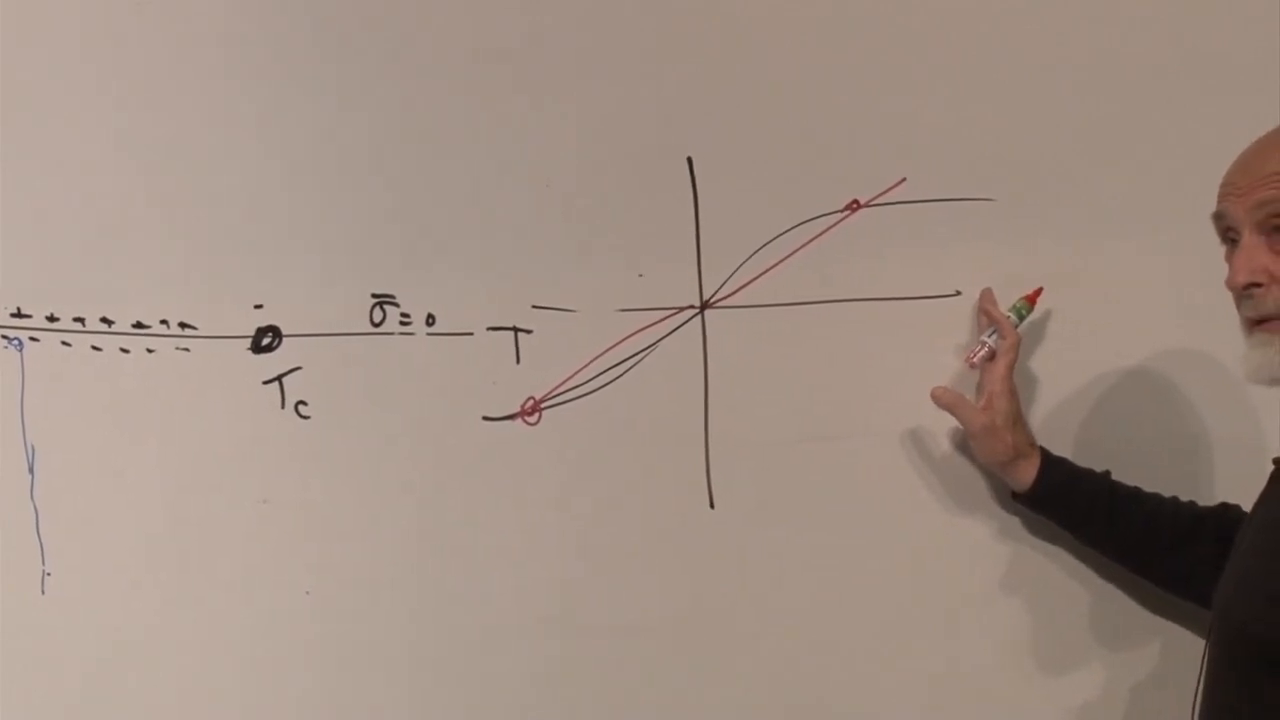
\includegraphics[width=0.90\textwidth]{lecture_10_figure_06.png}
\caption{\(T\)--\(h\) 面における共存線と、\(T_c\) 以下の固定温度における磁化の分枝。}
\lectureframe{00:39:30}
\end{figure}

\begin{figure}[ht]
\centering
\resizebox{\linewidth}{!}{%
\begin{tikzpicture}[x=1.25cm,y=1.15cm]
\begin{scope}
\draw[->] (-2.45,0) -- (2.55,0) node[right] {$h$};
\draw[->] (0,0) -- (0,3.7) node[above] {$T$};
\draw[very thick,red!70!black] (0,0) -- (0,2.35);
\fill[red!70!black] (0,2.35) circle (2.3pt);
\node[right] at (0.08,2.35) {$T_c$};
\node at (-1.25,1.05) {$m>0$};
\node at (1.25,1.05) {$m<0$};
\draw[->,rounded corners,blue!65!black] (-1.65,0.85) -- (-1.65,3.02)
 -- (1.65,3.02) -- (1.65,0.85);
\node[blue!65!black] at (0,3.35) {continuous path};
\end{scope}
\begin{scope}[xshift=7.0cm,yshift=1.55cm]
\draw[->] (-2.5,0) -- (2.5,0) node[right] {$h$};
\draw[->] (0,-1.35) -- (0,1.4) node[above] {$m$};
\draw[very thick,blue!65!black]
  (-2.2,1.05) .. controls (-0.75,1.03) and (-0.2,0.75) .. (-0.08,0.62);
\draw[very thick,blue!65!black]
  (0.08,-0.62) .. controls (0.2,-0.75) and (0.75,-1.03) .. (2.2,-1.05);
\draw[dashed] (0,0.62) -- (0,-0.62);
\fill (0,0.62) circle (1.8pt);
\fill (0,-0.62) circle (1.8pt);
\node at (0,-1.75) {\(T<T_c\)};
\end{scope}
\end{tikzpicture}
}
\caption{固定した \(T<T_c\) では、磁化は共存線を横切って跳ぶ。完全な二パラメータ面では、代わりに臨界点を回り込むことによって二つの相を連続的につなぐことができる。}
\label{fig:ising-phase-plane}
\end{figure}

\begin{classroomqa}
\audiencequestion{\(T_c\) 以下で磁場がちょうどゼロであると何が起こるか。}
\lecturerresponse{理想的な無限系は二つの等しく良好な純粋相をもつ。調製に伴う任意の無限小の残留バイアス、境界条件、または揺らぎが、その一方を選び出す。熱力学的な不連続性は、我々の符号の規約における二つの片側極限 \(m(T,0^-)=+m_0(T)\) と \(m(T,0^+)=-m_0(T)\) によって表される。\lecturetimestamp{00:35:04--00:37:10}}
\end{classroomqa}

\begin{classroomqa}
\audiencequestion{これはヒステリシスと同じことか。}
\lecturerresponse{ヒステリシスは準安定性と、実在系が分枝を切り替える際の履歴に依存した遅れに関わる。それは関連しているが、平衡相図を超えた動力学を必要とし、ここでは展開しない。\lecturetimestamp{00:37:11--00:37:20}}
\end{classroomqa}

\begin{classroomqa}
\audiencequestion{正の相と負の相を不連続性を横切らずにつなぐことができるか。}
\lecturerresponse{できる。温度を \(T_c\) より上に上げ、そこで磁場の符号を変え、再び温度を下げる。その経路は端点を回り込み、磁化は連続的に変化する。跳びが避けられないのは、固定した \(T<T_c\) で \(h=0\) を横切るときだけである。\lecturetimestamp{00:37:20--00:38:15}}
\end{classroomqa}

\begin{classroomqa}
\audiencequestion{\(h\) がゼロに近づくときはいつでも磁化はゼロに近づくか。}
\lecturerresponse{\(T_c\) 以下の一般的な温度ではそうではない。そこでは片側極限は非ゼロである。自発磁化がゼロに近づくのは、臨界温度そのものに近づくときだけである。\lecturetimestamp{00:38:29--00:39:45}}
\end{classroomqa}

\section{透過性の箱と化学ポテンシャル}

ここで磁石を離れ、再び粒子から始める。周囲の空間よりポテンシャルエネルギーが低い領域を想像しよう。壁は透過性である。すなわち粒子は出入りできる。内部のエネルギーが量 \(\mu\) だけ低いなら、内部の占有は相対的なボルツマン因子 \(e^{\beta\mu}\) を受け取る。井戸を深くしたり浅くしたりすると、箱の中の平均粒子数が変わる。

\begin{figure}[ht]
\centering
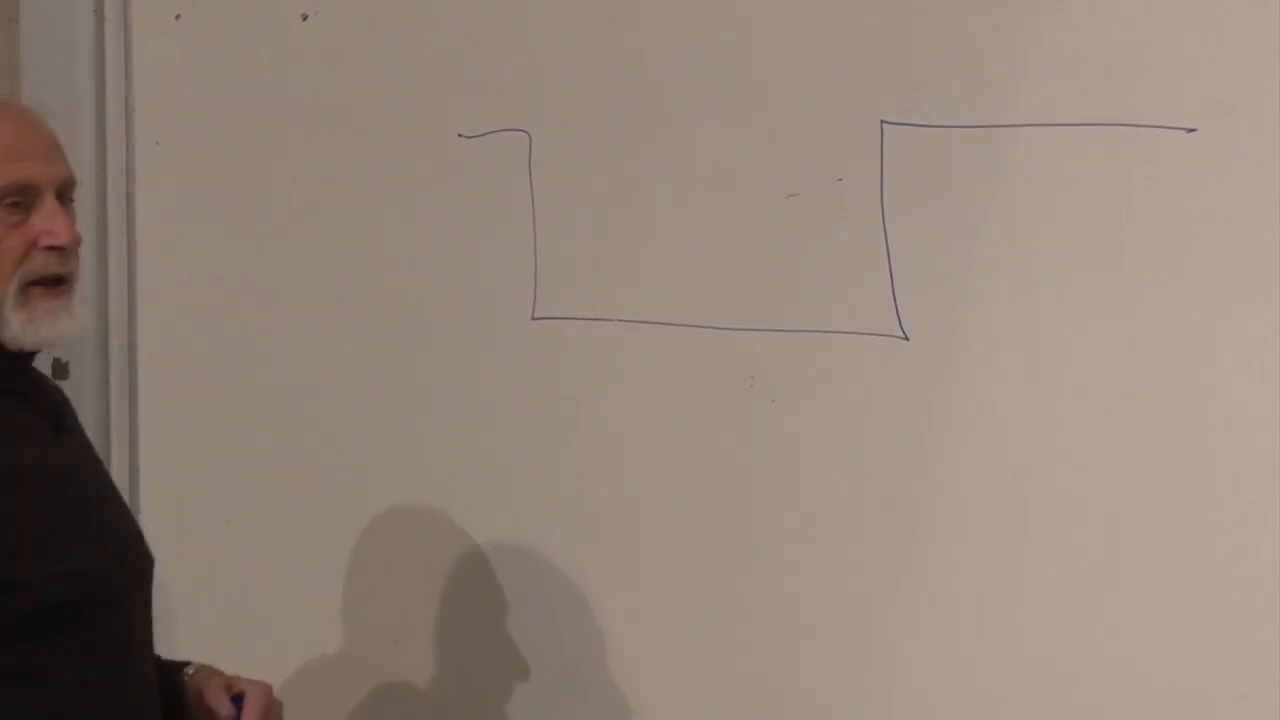
\includegraphics[width=0.84\textwidth]{lecture_10_figure_07.png}
\caption{透過性の箱のポテンシャル井戸の描像。内部と外部のエネルギー差が、粒子が箱を占める選好を制御する。}
\lectureframe{00:41:30}
\end{figure}

\begin{figure}[ht]
\centering
\resizebox{\linewidth}{!}{%
\begin{tikzpicture}[x=1.25cm,y=1.0cm]
\draw[->] (-3.2,0) -- (3.3,0) node[right] {position};
\draw[->] (-3.0,-2.4) -- (-3.0,1.2) node[above] {potential};
\draw[very thick] (-2.8,0.7) -- (-1.35,0.7)
 -- (-1.35,-1.45) -- (1.35,-1.45) -- (1.35,0.7) -- (2.9,0.7);
\draw[<->,red!70!black] (0,0.63) -- (0,-1.38);
\node[right,red!70!black] at (0.08,-0.35) {$\mu$};
\foreach \x/\y in {-0.95/-1.1,-0.45/-0.85,0.05/-1.12,0.55/-0.95,0.95/-1.18}
  \fill[blue!65!black] (\x,\y) circle (2pt);
\node at (0,-2.0) {permeable region};
\end{tikzpicture}
}
\caption{ポテンシャルのオフセットを変えると粒子数の選好が変わる。大正準記述では、そのオフセットは化学ポテンシャルによって表される。}
\end{figure}

この思考実験は化学ポテンシャルを具体的にする。それは貯蔵庫に対して加えられた粒子一つあたりのエネルギー上の利得である。複数の種が壁を通り抜けられるなら、各々の種がそれ自身の化学ポテンシャルをもつ。密閉された箱は異なる。その場合 \(N\) は固定され、化学ポテンシャルは貯蔵庫との交換によって課されるのではなく、熱力学的に推論される。

\begin{classroomqa}
\audiencequestion{井戸の深さは文字通り化学ポテンシャルか。}
\lecturerresponse{それは化学ポテンシャル差の直接的な力学的実現である。内部のすべての一粒子準位を \(\mu\) だけ下げることは、エネルギーに \(-\mu N\) を寄与し、したがってボルツマン指数に \(+\beta\mu N\) を寄与する。化学ポテンシャルの差だけが意味をもつ。\lecturetimestamp{00:44:49--00:45:40}}
\end{classroomqa}

粒子が出入りできるので、分配和はすべての粒子数を含まなければならない。
\begin{equation}
\Xi(T,\mu)
=\sum_{N=0}^{\infty}\;\sum_{\mathcal C_N}
\exp\!\left[-\beta E(\mathcal C_N)+\beta\mu N\right].
\label{eq:grand-partition}
\end{equation}
内側の和は指定された \(N\) をもつ配置にわたって走り、外側の和は \(N\) そのものにわたって走る。大正準重みは \(e^{-\beta(E-\mu N)}\) とも書ける。

\begin{figure}[ht]
\centering
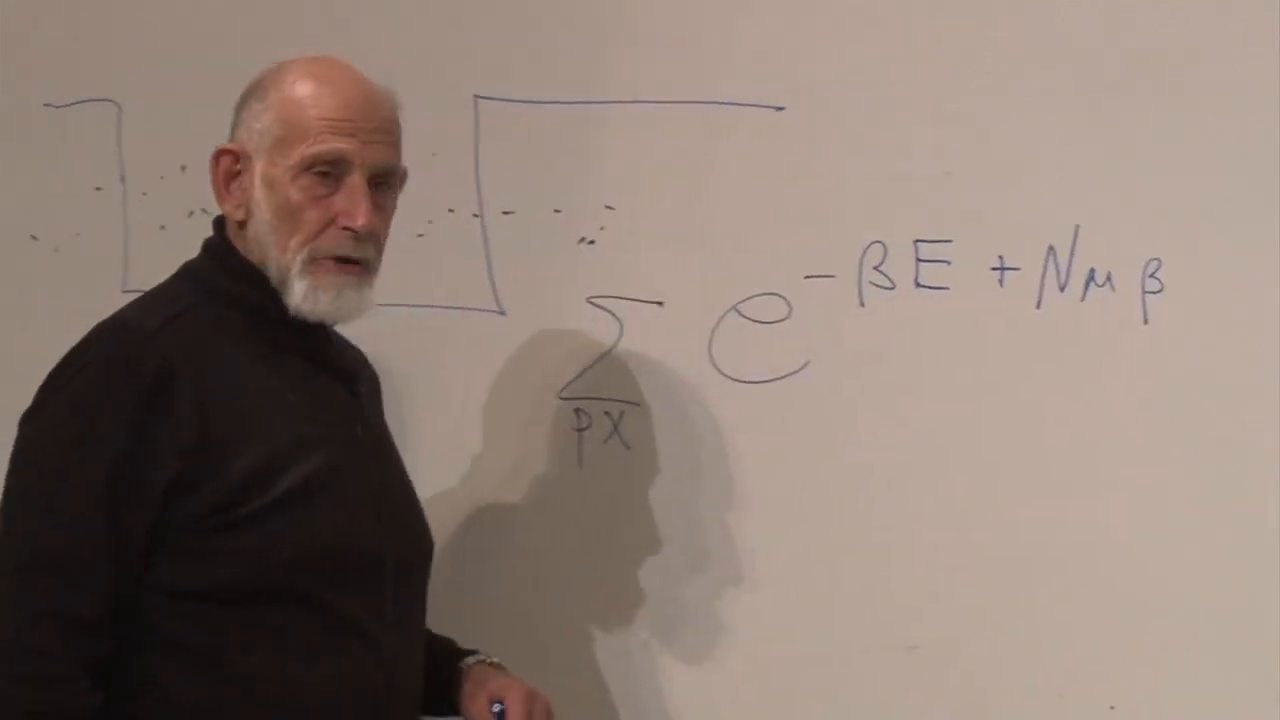
\includegraphics[width=0.88\textwidth]{lecture_10_figure_08.png}
\caption{透過性の箱と、粒子数および配置にわたる大正準和。}
\lectureframe{00:47:15}
\end{figure}

\begin{classroomqa}
\audiencequestion{箱が密閉されると何が変わるか。}
\lecturerresponse{粒子数は揺らがなくなる。そのとき固定した \(N\) における正準分配関数を用いる。透過性の箱では、\(N\) は \(\mu\) によって平均的に制御される熱力学変数である。\lecturetimestamp{00:45:42--00:47:50}}
\end{classroomqa}

一定温度では、\(\mu\)を変えると通常は密度が滑らかに変化する。臨界温度以下では、代わりに不連続な跳びを引き起こすことがある。それこそが我々の求めている流体現象である。これを微視的に得るには、粒子に二つの特徴が必要である。すなわち、同じ場所を占めることができてはならず、短距離で引き合わなければならない。

\section{スピンを格子気体に変える}

格子はそのままにして、その二つの状態を読み替える。占有数
\begin{equation}
n_i=\frac{1+\sigma_i}{2}
=
\begin{cases}
0,&\sigma_i=-1,\\
1,&\sigma_i=+1.
\end{cases}
\label{eq:occupation-map}
\end{equation}
を定義する。空のサイトはスピン下向き、占有されたサイトはスピン上向きである。\(n_i\)は0か1しかとれないので、二重占有は禁止される。したがって格子自体が剛体芯を与える。

\begin{figure}[ht]
\centering
\includegraphics[width=0.84\textwidth]{lecture_10_figure_04.png}
\caption{格子気体との対応付けは、\(\sigma=-1\)を空のサイトとすることから始まる。すると\(\sigma=+1\)は占有されたサイトである。}
\lectureframe{00:53:45}
\end{figure}

空の格子、すなわちすべて\(\sigma=-1\)から始める。すべての結合は揃っており、エネルギー\(-J\)をもつ。この一定の真空エネルギーは差し引くことができる。次に2次元で1個の粒子をサイトに置く。対応するスピンは\(+1\)に反転し、4本の結合を壊す。壊れた結合はそれぞれ\(2J\)のコストがかかるので、
\begin{equation}
\Delta E_1=4(2J)=8J.
\label{eq:one-particle-cost}
\end{equation}
遠く離れた2個の粒子は8本の結合を壊し、\(16J\)のコストがかかる。2個の粒子が隣接するサイトを占めるなら、それらの間の結合は再び揃う。壊れる境界結合は6本だけであり、コストは
\begin{equation}
\Delta E_{2,\rm adjacent}=6(2J)=12J.
\end{equation}
したがって粒子を近づけるとエネルギーが
\begin{equation}
16J-12J=4J.
\label{eq:lattice-attraction}
\end{equation}
だけ下がる。この生の数え上げは最初\(2J\)の節約として述べられ、その後訂正された。共有された1本の結合が壊れた境界への寄与を二つ取り除くので、引力は\(4J\)である。

\begin{figure}[ht]
\centering
\includegraphics[width=0.84\textwidth]{lecture_10_figure_05.png}
\caption{2次元の結合の数え上げ：孤立した1個の粒子は\(8J\)、遠く離れた2個の粒子は\(16J\)、隣接する2個の粒子は\(12J\)のコストがかかる。}
\lectureframe{01:00:25}
\end{figure}

格子気体は今や必要な分子論的性質を両方備えている。二値的な占有が剛体芯排除を与え、交換相互作用が強さ\(4J\)の最近接引力を与える。スピン反転が占有サイトの数を変えるので、粒子数は揺らぐことが許される。

\subsection{厳密な代数的対応辞書}

結合を数える描像で物理を見るには十分だが、変数変換を正確に行えば等価性は紛れもなくなる。
\begin{equation}
\sigma_i=2n_i-1
\end{equation}
を式~\eqref{eq:ising-hamiltonian}に代入する。リンクについて、
\begin{equation}
\sigma_i\sigma_j
=4n_in_j-2n_i-2n_j+1.
\end{equation}
正則な\(d\)次元格子では、
\begin{equation}
\sum_{\langle ij\rangle}(n_i+n_j)=2d\sum_i n_i.
\end{equation}
したがって
\begin{align}
\mathcal H
&=-4J\sum_{\langle ij\rangle}n_in_j
+(4dJ+2h)\sum_i n_i+\text{constant}.
\label{eq:ising-as-lattice-gas}
\end{align}
これを従来の格子気体ハミルトニアン
\begin{equation}
\mathcal H_{\rm lg}
=-\epsilon\sum_{\langle ij\rangle}n_in_j
-\mu\sum_i n_i+\text{constant}.
\label{eq:lattice-gas-hamiltonian}
\end{equation}
と比較する。対応関係は
\begin{equation}
\boxed{\epsilon=4J,\qquad
\mu=-(4dJ+2h).}
\label{eq:chemical-potential-map}
\end{equation}

\begin{figure}[ht]
\centering
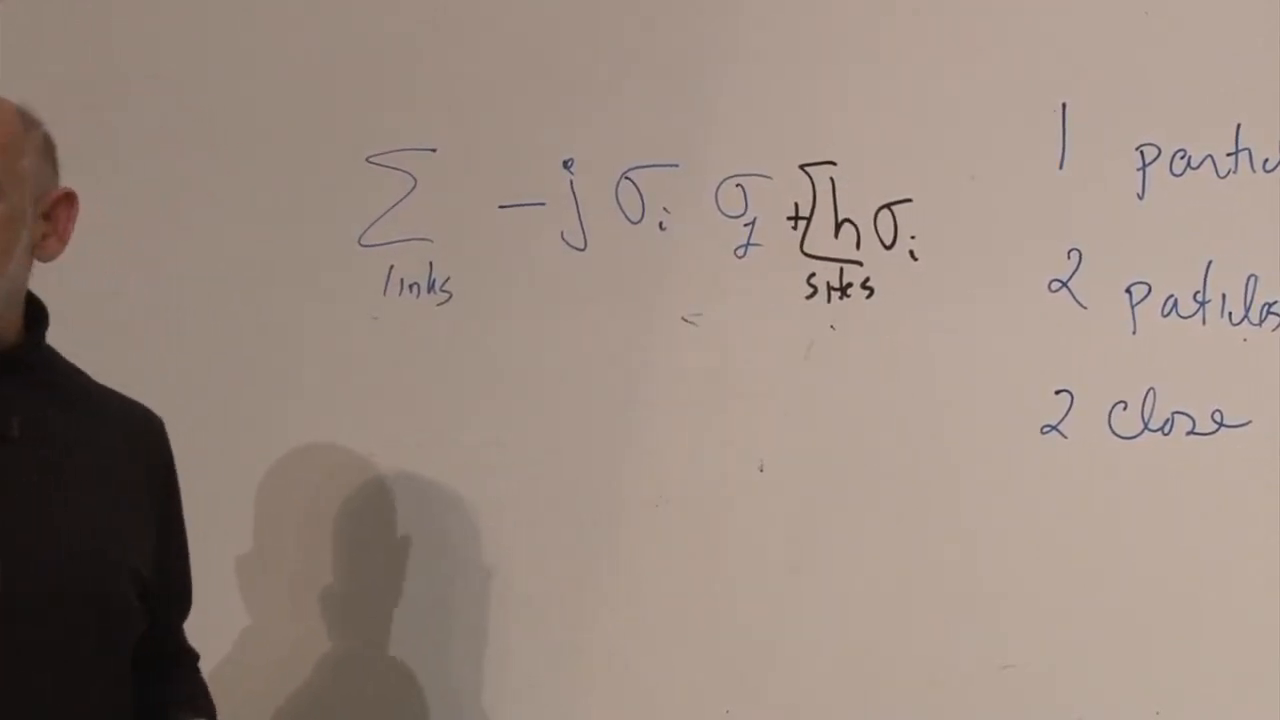
\includegraphics[width=0.88\textwidth]{lecture_10_figure_09.png}
\caption{粒子エネルギーの数え上げの隣に並べた交換項と場の項。場は最近接引力を変えずに挿入エネルギーを変える。}
\lectureframe{01:04:30}
\end{figure}

2次元では、孤立した挿入はエネルギーを
\begin{equation}
8J+2h=-\mu.
\end{equation}
だけ変える。\(8J\)は壊れた結合から来ており、\(2h\)は1個のスピンを\(-1\)から\(+1\)へ変えることから来る。したがって\(h\)を調整すると、引力\(4J\)を固定したまま化学ポテンシャルを調整することになる。場は文字通り\(\mu\)に等しいわけではない。交換の基準値がオフセット\(4dJ\)に寄与するからである。

\begin{classroomqa}
\audiencequestion{場が粒子数を制御するなら、なぜ\(h\)は単に化学ポテンシャルではないのか。}
\lecturerresponse{粒子を生成することは、空の参照状態に対して交換結合も壊す。したがって\(-N\)の従来の係数は\(\mu=-(4dJ+2h)\)であり、単に\(-2h\)ではない。オフセットは\(J\)と配位数に依存する。\lecturetimestamp{01:06:28--01:06:41}}
\end{classroomqa}

密度も同様に単純である。
\begin{equation}
\rho=\expect{n_i}
=\frac{1+\expect{\sigma_i}}{2}
=\frac{1+m}{2}.
\label{eq:density-map}
\end{equation}
したがって\(m=-1\)は空の格子、\(m=+1\)は完全に満たされた格子、\(m=0\)は半充填である。全粒子数は\(N_{\rm p}=\sum_i n_i\)であり、密度は\(N_{\rm p}/N\)である。

\begin{figure}[ht]
\centering
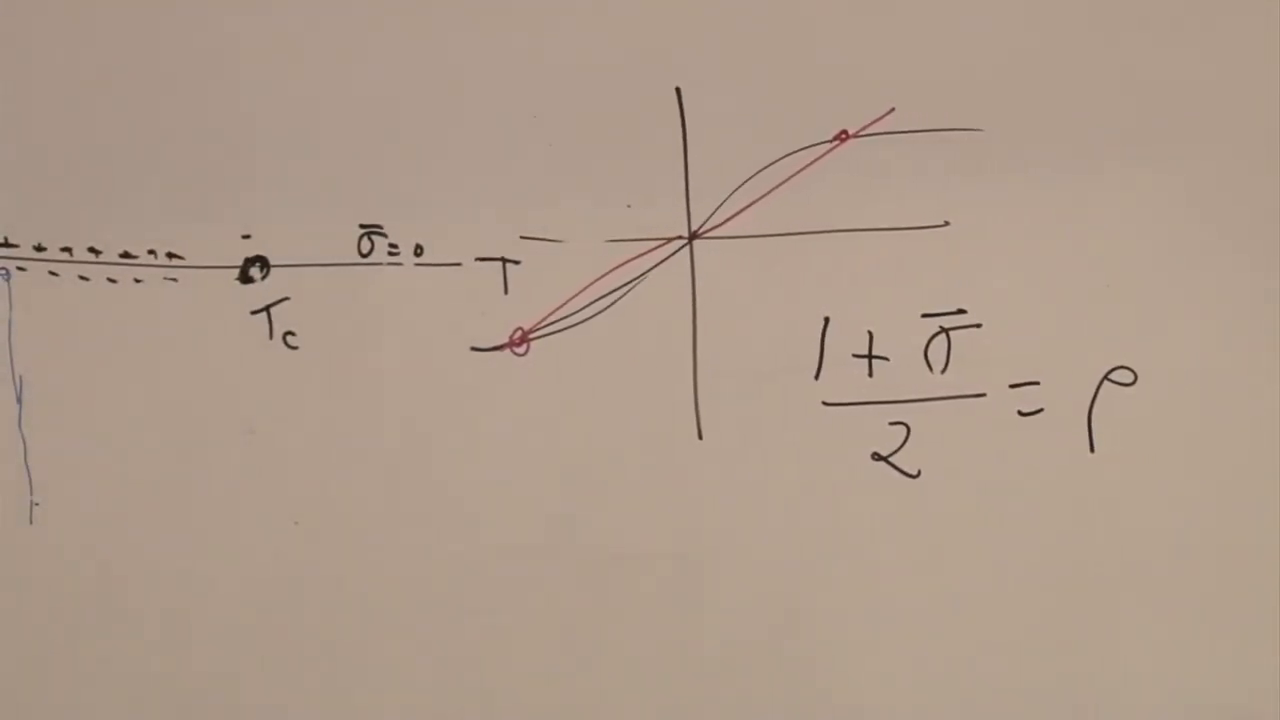
\includegraphics[width=0.90\textwidth]{lecture_10_figure_10.png}
\caption{磁気共存線の隣に書かれた密度関係\(\rho=(1+m)/2\)。}
\lectureframe{01:08:25}
\end{figure}

\begin{classroomqa}
\audiencequestion{\((1+m)/2\)は粒子数か、それとも密度か。}
\lecturerresponse{それはサイトあたりの平均占有数であり、したがって無次元の格子密度である。全サイト数を掛けると期待粒子数が得られる。示強的な密度と示量的な数え上げの区別は重要である。\lecturetimestamp{01:06:43--01:09:31}}
\end{classroomqa}

\section{磁気相図が流体相図になる}

式~\eqref{eq:chemical-potential-map}と\eqref{eq:density-map}を用いて図~\ref{fig:ising-phase-plane}を読み替える。\(T_c\)より上では、\(\mu\)を変えると密度が滑らかに変化する。\(T_c\)より下では、共存値
\begin{equation}
\mu_{\rm coex}=-4dJ
\qquad(h=0)
\label{eq:coexistence-mu}
\end{equation}
を横切ると密度が希薄気体と高密度液体の間で跳ぶ。\(T_c\)では二つの密度が合流し、不連続性が消える。

\begin{figure}[ht]
\centering
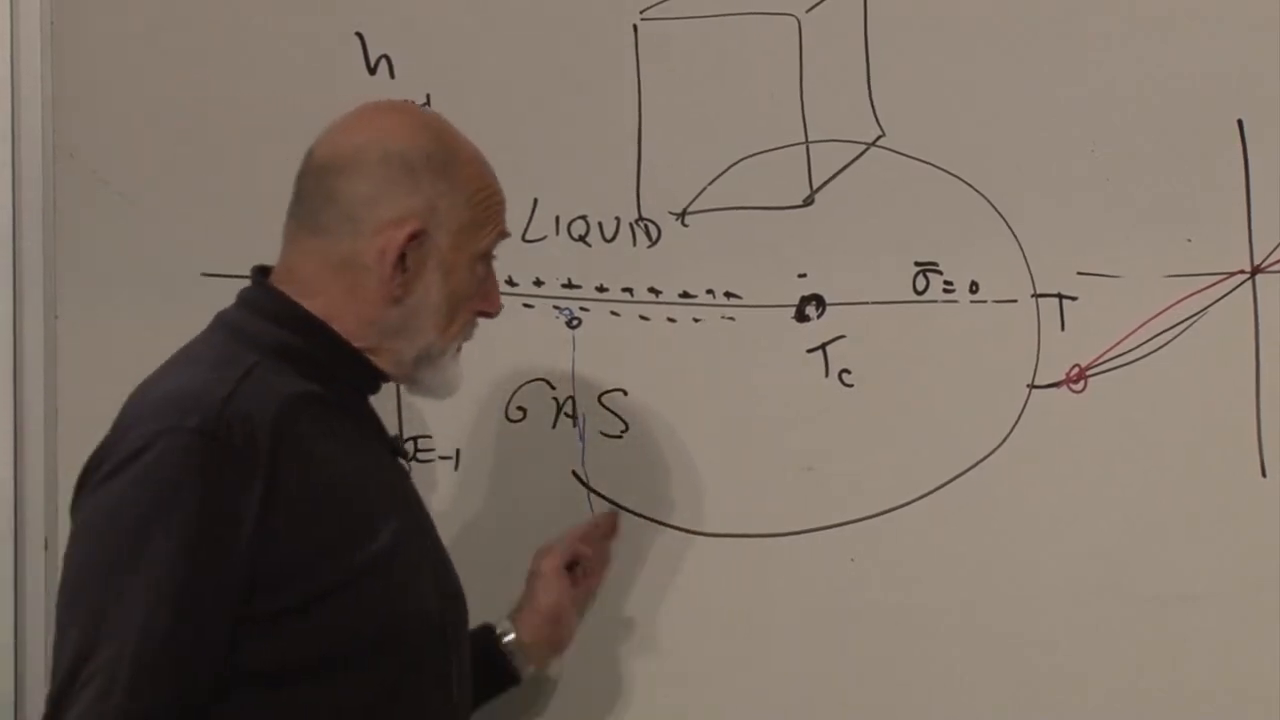
\includegraphics[width=0.92\textwidth]{lecture_10_figure_11.png}
\caption{Isingの共存線を液体--気体の相図として読む。気体は低密度側に、液体は高密度側にあり、両者は臨界端点の周りを連続的につなぐことができる。}
\lectureframe{01:14:30}
\end{figure}

\begin{figure}[ht]
\centering
\begin{tikzpicture}[x=1.25cm,y=1.1cm]
\draw[->] (-2.65,0) -- (2.75,0) node[right] {$\mu-\mu_{\rm coex}$};
\draw[->] (0,0) -- (0,3.8) node[above] {$T$};
\draw[very thick,red!70!black] (0,0) -- (0,2.35);
\fill[red!70!black] (0,2.35) circle (2.4pt);
\node[right] at (0.1,2.35) {critical point};
\node at (-1.35,1.0) {gas};
\node at (1.35,1.0) {liquid};
\draw[->,blue!65!black,rounded corners]
 (-1.7,0.85) -- (-1.7,3.05) -- (1.7,3.05) -- (1.7,0.85);
\node[blue!65!black] at (0,3.4) {continuous route};
\end{tikzpicture}
\caption{端点より下では液体と気体は別個の相であるが、超臨界領域ではそれらを隔てる特異な境界は存在しない。}
\label{fig:liquid-gas-plane}
\end{figure}

これはよく知られた沸騰線を同定する。一定の圧力のもとで液体を加熱し共存線を越えると沸騰が起こる。一定の温度のもとでは、圧力または化学ポテンシャルを変えることによって同じ境界を越えることができる。過熱蒸気や過冷却液体は平衡共存を越えた準安定な継続であり、その寿命を記述するには核生成の動力学が必要であって、それはこの平衡論的な構成の範囲を超えている。

\begin{classroomqa}
\audiencequestion{過熱蒸気はこの相図に表されているか。}
\lecturerresponse{平衡相図は共存境界を同定する。過熱状態または過飽和状態は準安定である。すなわち、臨界液滴を形成するには界面自由エネルギーのコストがかかるため、誤った側に一時的にとどまる。この動力学による精密化はここでは計算しない。\lecturetimestamp{01:12:19--01:12:29}}
\end{classroomqa}

\begin{classroomqa}
\audiencequestion{通常の流体では化学ポテンシャルをどのように変えるのか。}
\lecturerresponse{ポテンシャル井戸の箱が理論的に最も明快な制御である。実験室では圧力、体積、またはリザーバーとの接触を変えることのほうが多く、熱力学がそれらの制御を化学ポテンシャルの変化へと翻訳する。\lecturetimestamp{01:12:30--01:13:59}}
\end{classroomqa}

\begin{classroomqa}
\audiencequestion{密度が変化するとき、分子ポテンシャル\(J\)を変えているのか。}
\lecturerresponse{いいえ。固定された物質に対して、\(J\)は短距離引力を表し、この模型では固定されている。\(\mu\)を変えると、いくつのサイトが占有されるかが変わり、したがって分子間距離の分布が変わる。\(J\)を変えることは、微視的な物質または相互作用を変えることを意味する。\lecturetimestamp{01:14:50--01:15:41}}
\end{classroomqa}

\begin{classroomqa}
\audiencequestion{臨界温度は通常の沸点と同じものか。}
\lecturerresponse{いいえ。沸点は選ばれた圧力のもとで指定されるので、圧力が変われば共存曲線に沿って移動する。臨界温度は、それを超えると液体と気体がもはや相境界によって隔てられなくなる唯一の端点である。この格子気体の扱いでは圧力は陽に導出されていない。\lecturetimestamp{01:15:42--01:17:02}}
\end{classroomqa}

ここで中心的な結果を述べることができる。Ising磁性体と格子気体は単に似た図を描くだけではない。変数とパラメータの変換の後、それらは分配関数を共有する。一方の側のすべての特異な熱力学的性質は、他方の側に対応するものをもつ。
\begin{equation}
\begin{array}{c|c}
\text{Ising magnet} & \text{lattice gas}\\ \hline
\sigma_i=\pm1 & n_i=0,1\\
m=\expect{\sigma} & \rho=(1+m)/2\\
h & \mu=-(4dJ+2h)\\
\text{aligned exchange} & \text{nearest-neighbor attraction}\\
h=0,\ T<T_c & \text{liquid--gas coexistence}\\
(T_c,0) & \text{critical endpoint}
\end{array}
\label{eq:ising-fluid-dictionary}
\end{equation}

\section{臨界指数と普遍性}

臨界点の近くでは、熱力学的量はしばしば冪則的な特異性を示す。換算温度
\begin{equation}
t=\frac{T-T_c}{T_c},
\end{equation}
を用いて、模式的には次のように書ける。
\begin{equation}
m\sim(-t)^{\beta_{\rm crit}},
\qquad
\chi\sim |t|^{-\gamma},
\qquad
\xi\sim |t|^{-\nu}.
\label{eq:critical-exponents}
\end{equation}
ここで\(\beta_{\rm crit}\)は臨界指数であり、逆温度ではない。平均場では\(\beta_{\rm crit}=1/2\)を与えるが、揺らぎは上限臨界次元より下で指数を変える。

指数は整数である必要はない。またすべてが無理数である必要もない。二次元Ising模型は有名なことにいくつかの厳密な有理指数をもつ一方、三次元Isingの値は理論と計算によって高い精度で決定された非自明な数である。頑健な教訓は、指数は一般に初等的な次元解析によって固定されるものではないということである。

さらに驚くべきことに、微視的な詳細がそれらを固定しないことが多い。同じ空間次元、同じ秩序変数の対称性、そして十分に短距離の相互作用をもつ系は、同じ長距離臨界理論へと流れることができる。それらは一つの\emph{普遍性クラス}に属する。一軸磁性体と通常の液体--気体端点はどちらも単一のスカラー秩序変数をもち、同じ次元のIsing普遍性クラスを共有する。

\begin{classroomqa}
\audiencequestion{普遍性クラスは有限または離散的なリストなのか。}
\lecturerresponse{多くのクラスがあり、次元、対称性、保存則、相互作用の到達距離、その他の長距離的データによって組織される。多くのよく知られた場合では固定点と指数の組は離散的であるが、指数が連続的に変化する系も存在する。安全な主張は、目録が有限であるということではなく、多くの微視的に異なる系が同じ長距離的データを共有するということである。\lecturetimestamp{01:18:50--01:19:38}}
\end{classroomqa}

\begin{classroomqa}
\audiencequestion{液体と気体が共存するとき、実際の容器の中で両者を隔てているものは何か。}
\lecturerresponse{界面である。表面張力は界面の面積にペナルティを与え、重力は鉛直方向の化学ポテンシャル勾配を生み出し、通常はより密度の大きい液体を気体の下に置く。無視できる重力のもとでは、幾何学的配置は表面張力と境界条件によってより直接的に支配される。\lecturetimestamp{01:19:40--01:21:18}}
\end{classroomqa}

\begin{classroomqa}
\audiencequestion{この描像において気化熱はどこにあるのか。}
\lecturerresponse{臨界点より下では、一次相転移の共存線を横切ることは一般に潜熱を伴う。二つの相がそこで同一になるため、臨界端点に近づくにつれて気化熱はゼロに近づく。この講義は相構造を確立するが、潜熱を計算するものではない。\lecturetimestamp{01:21:19--01:22:18}}
\end{classroomqa}

\begin{classroomqa}
\audiencequestion{相転移を、例えば超伝導デバイスを用いて、敏感な検出器として使うことができるか。}
\lecturerresponse{できる。転移の近くでは、小さな摂動が大きな応答を生み出したり、状態の変化を引き起こしたりしうる。実用的な検出器はその感度を利用するが、関係する秩序変数やダイナミクスはイジングの例とは異なるかもしれない。\lecturetimestamp{01:22:19--01:24:05}}
\end{classroomqa}

これで統計力学の講義を終える。その道筋はエントロピーと平衡から始まり、分配関数と気体を経て、磁石と流体が同一の臨界現象の二つの記述でありうることを示して終わる。

\section{講義後の議論：微調整と選択}

正式な講義が終わった後、会話はおよそ四十分にわたって続いた。それは記録に残す価値があるが、上記の導出と混同されるべきではない。主題はもはや格子気体ではない。それは微調整の論理と、宇宙論における人間原理的選択の慎重な使用である。

\subsection{小さな数は自動的に微調整されているわけではない}

\emph{人間原理}という語句のあらゆる用法を決着させる単一の文は存在しない。有用な出発点は操作的である。すなわち、ある理論が多数の実現された環境を許すとき、観測は、観測者が生じうるのはそれらの一部においてのみであるという事実に条件づけられる。その条件付きの言明は合理的でありうる。しかし、アンサンブル、選択条件、あるいは代替案を物理的に意味あるものにする機構を伴わずに持ち出されるならば、それは空虚になる。

選択が入り込む前に、小さなパラメータと微調整されたパラメータとを区別しなければならない。ある数が小さいのは、安定な力学的機構がそれを特別な値へと駆動するからでありうる。微調整とは、観測された値が、それ以外では独立な寄与の間の並外れて精密な釣り合いを要求しているように見え、その釣り合いを保護する既知の復元機構も対称性も存在しないことを意味する。

\begin{classroomqa}
\audiencequestion{人間原理は鋭く述べることができるか。}
\lecturerresponse{その擁護可能な用法は、神秘的というよりも条件付きである。すなわち、多数の物理的に実現された環境が異なるパラメータをもつならば、我々のような存在によって観測される環境は、観測者と両立する部分集合から引き出される。そのこと自体は環境を生成したり、それらの確率を割り当てたりするものではない。それらの課題は根底にある物理学に属する。\lecturetimestamp{01:25:45--01:26:13}}
\end{classroomqa}

宇宙定数はその動機となる例である。その観測された大きさは、真空エネルギーへの素朴な量子場理論的寄与と比べて並外れて小さい。困難は、単に最終的な数が小さいことではない。多くの大きな項が途方もない精度で相殺しなければならないように見える一方で、結果を観測値へと調整する、受け入れられた低エネルギー・フィードバック機構が存在しないことである。

\subsection{飛行船と潜水艦}

二つの浮力の例がこの区別を際立たせる。飛行船は、その平均密度が周囲の空気の密度と一致する高度に浮かぶ。空気の密度は高度とともに減少する。飛行船が上昇すれば、外部の空気はより希薄になり、飛行船は下降しようとする。下降すれば、外部の空気はより密になり、飛行船は上昇しようとする。密度の一致は数値的に微妙でありうるが、大気の勾配が復元フィードバックを与える。この平衡は力学的に説明される。

ほぼ非圧縮性の水中で中性浮力をとる潜水艦は異なる。水の密度は深さによってほとんど変化しない。潜水艦の平均密度がたまたま周囲の水と等しくなったとしても、その等しさを説明する、深さに依存する同程度の復元機構は存在しない。わずかな不一致が潜水艦を上昇させたり沈めたりする。中性浮力を達成するには、バラストと内容物の精密な調整が必要である。そのとき、何らかの制御系や設計機構がそれを説明しない限り、小さな残差は微調整である。

\begin{figure}[ht]
\centering
\resizebox{\linewidth}{!}{%
\begin{tikzpicture}[>=Latex]
\begin{scope}[xshift=-3.8cm]
\shade[top color=blue!5,bottom color=blue!28] (-2.5,-2.2) rectangle (2.5,2.2);
\draw[very thick,rounded corners=18pt,fill=yellow!35]
  (-1.15,0) ellipse (1.15 and 0.55);
\draw[thick] (0,-0.55) -- (0,-1.05);
\draw[thick,fill=gray!20] (-0.45,-1.05) rectangle (0.45,-1.38);
\draw[->,red!70!black,thick] (1.65,1.45) -- (1.65,0.55)
 node[midway,right] {restoring};
\draw[->,red!70!black,thick] (-1.65,-1.45) -- (-1.65,-0.55)
 node[midway,left] {restoring};
\node at (0,2.55) {\textbf{Blimp: density gradient}};
\node[align=center] at (0,-2.75) {displacement changes\\the buoyant imbalance};
\end{scope}
\begin{scope}[xshift=3.8cm]
\shade[top color=cyan!10,bottom color=blue!45] (-2.5,-2.2) rectangle (2.5,2.2);
\draw[very thick,fill=gray!35,rounded corners=12pt]
  (-1.45,-0.25) -- (1.1,-0.25) arc (-90:90:0.38)
  -- (-1.45,0.51) -- cycle;
\draw[thick] (-0.25,0.51) -- (-0.25,0.85) -- (0.35,0.85) -- (0.35,0.51);
\draw[->,red!70!black,thick] (1.65,0.15) -- (1.65,1.35)
 node[midway,right] {rise};
\draw[->,red!70!black,thick] (-1.65,0.15) -- (-1.65,-1.35)
 node[midway,left] {sink};
\node at (0,2.55) {\textbf{Submarine: nearly uniform density}};
\node[align=center] at (0,-2.75) {no depth-dependent feedback\\protects neutral buoyancy};
\end{scope}
\end{tikzpicture}
}
\caption{小さな残差は、力学的に安定でありうるし、真に調整されたものでもありうる。飛行船には復元フィードバックがあるが、理想化された潜水艦では、その平均密度を水に合わせて調整する必要がある。}
\label{fig:blimp-submarine}
\end{figure}

\begin{classroomqa}
\audiencequestion{中性浮力が観測されたなら、なぜ潜水艦の乗員は説明を要求すべきなのか。}
\lecturerresponse{バラスト制御機構がなければ、対称性も環境フィードバックも、二つの独立な密度の等しさを保護しないからである。問題は、その等しさが論理的に可能かどうかではなく、なぜ系がそのパラメータ空間のごく狭い領域を占めるのかである。\lecturetimestamp{01:35:05--01:36:25}}
\end{classroomqa}

\subsection{多数の領域と条件付き観測}

ここで、多くの異なる平均密度をもつ膨大な数の潜水艦を生成する過程を想像しよう。大半は沈むか浮き上がり、ごく一部だけが水面と海底の間の居住可能帯にとどまる。必然的に生き残った潜水艦の一つに住む観測者は、ほぼ中性の浮力を測定しても驚くべきではない。その観測は、観測者が存在するために必要な条件によって選択されている。

この推論には二つの要素が必要である。
\begin{enumerate}
\item 想像の中にのみ存在する代替案ではなく、実際に多くの代替案を実現する物理的過程。
\item なぜ観測が制限された部分集合においてのみなされるのかを説明する選択条件。
\end{enumerate}
選択は生成機構を置き換えるものではない。それは、アンサンブルが存在したときに観測者が何を測定するかの条件付き確率を変える。

\begin{classroomqa}
\audiencequestion{この議論は、十分に大きな標本のどこかで起こる unlikely な事柄にすぎないというものか。}
\lecturerresponse{それは前半にすぎない。後半は観測的条件付けである。観測者はすべての領域から一様に抽出されるのではなく、その存在が可能な領域からのみ抽出される。完全な提案には依然として、領域上の測度と、それらがどのように生成されるかの物理的説明が必要である。\lecturetimestamp{01:39:19--01:40:36}}
\end{classroomqa}

真空エネルギーに適用すると、大きな負の宇宙定数は宇宙を急速に再収縮させうるが、十分に大きな正の値は物質が銀河へ凝縮するのを妨げうる。観測値は、長寿命の構造と両立する狭い範囲にある。これは可能な選択条件を与えるが、宇宙定数の分布の導出ではない。

量子場の理論は微調整問題を付け加える。異なる場とスケールからの真空寄与は、それぞれが観測された残差よりはるかに大きい。それらの項がほぼ正確に相殺するなら、結果は自己修正する飛行船というより、注意深く釣り合わされた潜水艦に似る。この類推は論理的問題を明らかにするためのものであり、その解決を与えるためのものではない。

\begin{classroomqa}
\audiencequestion{一つのパラメータの変化を、他のいくつかのパラメータの変化で補償できるか。}
\lecturerresponse{できる。生存可能な集合は一つの軸上の狭い区間である必要はなく、多次元パラメータ空間内の薄い面でありうる。相関した変化は構造を保ちうるが、そのとき問題は、なぜ実現したパラメータがその面の近くにあるのか、また基礎理論がそれにどのような測度を割り当てるのかである。\lecturetimestamp{01:45:10--01:46:19}}
\end{classroomqa}

\begin{figure}[ht]
\centering
\begin{tikzpicture}[x=1.3cm,y=1.05cm,>=Latex]
\draw[->] (-3.2,0) -- (3.4,0) node[right] {$\lambda_1$};
\draw[->] (0,-2.5) -- (0,2.65) node[above] {$\lambda_2$};
\fill[gray!12] (-3,-2.25) rectangle (3.1,2.3);
\draw[very thick,blue!65!black]
 (-2.8,-1.55) .. controls (-1.3,-0.75) and (0.15,0.05) .. (2.85,1.55);
\draw[very thick,blue!25]
 (-2.8,-1.25) .. controls (-1.3,-0.45) and (0.15,0.35) .. (2.85,1.85);
\fill[blue!15,opacity=.65]
 (-2.8,-1.55) .. controls (-1.3,-0.75) and (0.15,0.05) .. (2.85,1.55)
 -- (2.85,1.85) .. controls (0.15,0.35) and (-1.3,-0.45) .. (-2.8,-1.25) -- cycle;
\node[blue!65!black,rotate=28] at (1.3,0.95) {viable band};
\foreach \x/\y in {-2.4/1.45,-1.7/-1.8,-0.9/1.8,0.3/-1.45,1.2/1.85,2.4/-0.8}
  \fill[red!65!black] (\x,\y) circle (2pt);
\fill[green!45!black] (0.55,0.58) circle (2.8pt);
\node[green!35!black,right] at (0.65,0.55) {observed domain};
\end{tikzpicture}
\caption{複数のパラメータがある場合、居住可能性や構造的生存可能性は、一つのパラメータの狭い区間ではなく、薄い相関帯を占めうる。選択は観測をその帯に制限するが、パラメータ分布を生成するわけではない。}
\label{fig:viable-parameter-band}
\end{figure}

\subsection{ランドスケープ提案とその不確実性}

代替案の一つの提案された源は、多くの準安定真空をもち、おそらく異なる宇宙論的領域に分布する理論である。弦理論のランドスケープの考えや永久インフレーションのシナリオが例であるが、その詳細な実現と確率測度は依然として不確かである。講義はこれを確立した事実ではなく、一つの可能性として提示している。

対称性が宇宙定数を正確にゼロに強制するなら、それはより従来型の説明であろう。困難は、観測された加速膨張が小さな非ゼロ値に対応することである。自然に正確にゼロを与える機構は、自動的に微小な残差を説明するわけではない。対称性の破れは、単に微調整を再導入しうる。ここで潜水艦の比喩が戻ってくる。ロープはそれを選ばれた深さに保ちうるが、その場合ロープこそが、仮定されるのではなく同定されねばならない機構である。

\begin{classroomqa}
\audiencequestion{パラメータを非常に精密に測定することは不確定性原理に違反するのか。}
\lecturerresponse{いいえ。不確定性関係は、指定された非可換な観測量の対に適用される。結合定数や真空のパラメータは、制御されていない観測量の正準共役でなくても、鋭く定義された値をもちうる。精密さそれ自体は不確定性原理のパラドックスではない。 \lecturetimestamp{01:49:21--01:49:36}}
\end{classroomqa}

\begin{classroomqa}
\audiencequestion{人間原理的な推論はその値を説明するのか、それとも観測者にそれが要求されるということを言い換えているだけなのか。}
\lecturerresponse{選択だけでは力学的な説明にはならない。その正当な役割は、物理的に実現されたアンサンブルにおける条件付き確率を変えることである。アンサンブル、測度、検証可能な帰結なしに用いられると、説明ではなくラベルになりかねない。 \lecturetimestamp{01:49:37--01:50:21}}
\end{classroomqa}

\subsection{素粒子物理学における中程度の偶然の一致}

生命に関わるパラメータのすべてが同じ並外れた度合いに調整されているわけではない。身近な物質は光子、電子、軽いクォーク、強い相互作用に依存しており、ニュートリノは宇宙論に影響するが原子の直接の結合要因ではない。陽子--中性子の質量差はとりわけ重要である。中性子が陽子よりわずかに重いため、孤立した中性子は崩壊しうるし、通常の水素は安定である。この順序を十分に逆転させれば、核化学は根本的に変わるであろう。

電子の質量と微細構造定数も同様に原子の大きさと結合エネルギーを定める。それらを大きく変えれば化学は変わるであろう。これらは意味のある感度に関する記述であるが、あらゆる小さな変動があらゆる想像しうる複雑さの形態を禁じるという主張に膨らませるべきではない。宇宙定数の問題と比べれば、そのような偶然の一致の多くは中程度であり、他のパラメータと相関している。

電弱スケールに関連する階層性は、もう一つの際立った自然さの問題である。放射補正は、追加の構造によって保護されない限り、基本的なスカラー質量を高いスケールに敏感にしがちである。その地位と解釈は真空エネルギーの問題とは異なり、どちらもスローガンに還元すべきではない。

\begin{classroomqa}
\audiencequestion{陽子--中性子の質量差を変えることは、通常の物質にとって本当に重要だろうか。}
\lecturerresponse{はい。観測されている順序は安定な水素を可能にし、原子核全体にわたるベータ安定性を支配する。適度な変化は核の存在量と恒星の燃焼を再編しうる。注意深い解析では、一つの数を変えながら他をすべて固定するのではなく、結合したパラメータを整合的に変化させなければならない。 \lecturetimestamp{01:51:47--01:53:08}}
\end{classroomqa}

\begin{classroomqa}
\audiencequestion{電子の質量と微細構造定数はどのような役割を果たすのか。}
\lecturerresponse{それらは特徴的な原子のエネルギーと長さのスケールを定め、模式的には \(E_{\rm atom}\sim \alpha^2m_e\) および \(a_0\sim(\alpha m_e)^{-1}\) を単位 \(\hbar=c=1\) として与える。大きな変化は化学を変えるであろうが、正確に生存可能な領域は多次元の問題である。 \lecturetimestamp{01:53:09--01:54:12}}
\end{classroomqa}

\subsection{不一致、時間依存性、検証}

議論はインフレーションへの批判と精密宇宙論データの解釈へと短く移る。その歴史的な不一致は、決着したものとしてではなく不一致として提示されるべきである。インフレーションには成功した現象論的予言と多くの模型の変種があり、初期条件、測度、検証可能性に関する問いは今も活発である。データは模型を制約するが、ある実験への単一の会話上の言及が枠組み全体を決着させることはない。

\begin{classroomqa}
\audiencequestion{宇宙定数は一定ではなく、時間とともにゆっくり変化しうるのか。}
\lecturerresponse{力学的な暗黒エネルギー場は時間依存の加速を生みうる。それはそれ自体が説明されねばならないポテンシャルと初期条件を導入し、観測は状態方程式が宇宙定数に近いことを制約する。講義当時の議論では、有意な時間変化を必要とする証拠はなかった。 \lecturetimestamp{01:57:17--01:59:19}}
\end{classroomqa}

\begin{classroomqa}
\audiencequestion{人間原理的な選択それ自体が異なる宇宙や領域を核生成するのか。}
\lecturerresponse{いいえ。選択は、どの実現された領域が観測者を含みうるかを述べるのであって、領域を創り出すのではない。インフレーションの歴史における真空遷移のような別個の宇宙論的機構がそれらを生成しなければならないだろう。 \lecturetimestamp{01:59:20--01:59:42}}
\end{classroomqa}

因果的な順序は明確に保たれなければならない。
\begin{equation}
\begin{gathered}
\text{laws and initial conditions}\\[-0.15em]
\downarrow\\[-0.15em]
\text{physical environments}\\[-0.15em]
\downarrow\\[-0.15em]
\text{observers and observations}
\end{gathered}
\end{equation}
観測者が過去に遡って法則を指図するのではない。条件付けは、実現された環境から引き出された観測者が何を測定しそうかと問うときに立ち入るのである。

したがって、科学的な問いは、その言語が哲学的、政治的、あるいは宗教的に響くかどうかではない。提案が定義された物理的アンサンブル、計算可能か少なくとも制約された測度、そして代替案と区別しうる帰結を備えているかどうかである。多真空宇宙論について議論された可能なシグネチャには、泡領域間の衝突の痕跡が含まれる。そのような信号を頑健に予測することは難しく、講義当時の議論では宇宙マイクロ波背景放射において確立されたものはなかった。容易な検証が存在しないことは深刻な限界であり、そのアイデアを真であると宣言したり、根底にある微調整問題を却下したりする免許ではない。

\begin{classroomqa}
\audiencequestion{何がこれを選択の議論から科学理論へと変えるのか。}
\lecturerresponse{その提案には、代替案を生成する機構、確率測度または制御された代替物、そして観測可能な帰結が必要である。泡衝突のシグネチャは一つの可能な道筋であるが、その不在または曖昧さは、検証可能性の問題がいかに厳しいかを示している。\lecturetimestamp{02:02:31--02:04:12}}
\end{classroomqa}

講義後のやり取りはその規律ある調子で終わる。微調整は、説明が欠けているかもしれないことの証拠である。対称性、動的調整、環境選択は、論理的に異なる候補説明である。選択は合理的でありうるが、それは仮定と限界が公然と述べられた物理的説明の一構成要素としてのみである。

\end{document}